\documentclass[../main/main.tex]{subfiles}
\begin{document}

%%%%%%%%%%%%%%%%%%%%%%%
%%%%%%%% LECTURE 16 PART 2 %%%%%%%%
%%%%%%%%%%%%%%%%%%%%%%%

\chapter{Vortices}

\cite[Chapter 3]{Shifman:2012}\\

The second quantum soliton that we consider is the vortex in $2+1$ dimensions in a model that in high-energy \emph{Abelian Higgs mode} and in $3+1$ dimensions was the first model proposed to make massive gauge fields in a gauge theory without losing gauge-invariance. 

In its non-relativistic version in condensed matter it described by the \emph{Landau-Ginzburg model} and in 3 space dimensions it was proposed as a phenomenological model for superconductors. 

Our discussion will be performed in the Lagrangian formalism, starting from the classical model. 

\section{Classical treatment}

\subsubsection{The classical Lagrangian}

The field content is made of a complex scalar field $\phi$ (whose complex conjugate is denote by $\phi^*$) and a $U(1)$ gauge field $A_\mu$. The classical relativistic Lagrangian is 
\begin{eq}\label{eq:lag-vortex}
	\lag=-\frac1{4e^2}F_{\mu\nu}^2+\vert D^\mu\phi\vert^2-\lambda(\vert\phi\vert^2-v^2)^2
\end{eq}
where $e$ is the electric charge, the covariant derivative is defined by
\begin{eq}
	D_\mu\phi=(\partial_\mu-in_eA_\mu)\phi
\end{eq}
and $n_e$ is the electric charge of $\phi$ in units of $e$. 

The non-relativistic Euclidean version replaces $\vert D^0\phi\vert^2$ by a first order term
\begin{eq}
	\vert D^0\phi\vert^2
	\quad\to\quad
	\phi^*(\partial_0-in_eA_0)\phi
\end{eq}

For the model of superconductivity $\phi$ is a field representing the large distance behaviour of the Cooper pairs generated by phonon attraction and $n_e\equiv2$. 
The vortices that will be discusse later in fact really appear in nature. 

\subsubsection{Application of vortices}

A lattice version of such vortices, called \emph{Abrikosov\footnote{Nobel prize in the 2003.} vortices}, is the equilibrium state of a class of superconductors in the presence of a magnetic field, orthogonal to the surface of the superconductors, whose direction will be denoted by $z$. The $z$-dependence is then trivial, and in the gauge $A_z=0$ the $3+1$ model reduces to a $2+1$ model. 

Notice that a typical characteristics of superconductors is the expulsion of the magnetic field (\emph{Meissner effect}), but there are two behaviours of superconducting materials in this respect, called \emph{type I} and \emph{type II}. In type I the magnetic flux is completely expelled from the bulk of the material, whereas in type II it penetrates in the superconductor in tubes whose two-dimensional cross section are the vortices, as shown in fig.~\ref{fig:vortices-type-II-superconductor}. Each of these tubes contains a flux $\frac he$ and at equilibrium if they are sufficiently many\footnote{In order to increase the number of tubes one can increase the strength of the magnetic field.} they are arranged in a triangular lattice, the \emph{Abrikosov lattice}. 

\begin{figure}[h]
\centering

% Pattern Info
\tikzset{
pattern size/.store in=\mcSize, 
pattern size = 1.275pt,
pattern thickness/.store in=\mcThickness, 
pattern thickness = 0.3pt,
pattern radius/.store in=\mcRadius, 
pattern radius = 0pt}
\makeatletter
\pgfutil@ifundefined{pgf@pattern@name@BottomEllipsesPattern}{
\pgfdeclarepatternformonly[\mcThickness,\mcSize]{BottomEllipsesPattern}
{\pgfqpoint{0pt}{-\mcThickness}}
{\pgfpoint{\mcSize}{\mcSize}}
{\pgfpoint{\mcSize}{\mcSize}}
{
\pgfsetcolor{\tikz@pattern@color}
\pgfsetlinewidth{\mcThickness}
\pgfpathmoveto{\pgfqpoint{0pt}{\mcSize}}
\pgfpathlineto{\pgfpoint{\mcSize+\mcThickness}{-\mcThickness}}
\pgfusepath{stroke}
}}
\makeatother     

\begin{tikzpicture}[x=0.75pt,y=0.75pt,yscale=-1,xscale=1]

%Shape: Cube [id:dp5322921626189492] 
\draw   (11,90.5) -- (96,5.5) -- (382,5.5) -- (382,125.5) -- (297,210.5) -- (11,210.5) -- cycle ; \draw   (382,5.5) -- (297,90.5) -- (11,90.5) ; \draw   (297,90.5) -- (297,210.5) ;

%Shape: Spring [id:dp0701641501341086] 
\draw  [dash pattern={on 1pt off 0.5pt}, line width=0.5] (41.39,79.83) .. controls (41.39,85.34) and (35.43,85.34) .. (35.43,83.17) .. controls (35.43,81) and (41.39,81) .. (41.39,86.51) .. controls (41.39,92.02) and (35.43,92.02) .. (35.43,89.85) .. controls (35.43,87.68) and (41.39,87.68) .. (41.39,93.19) .. controls (41.39,98.7) and (35.43,98.7) .. (35.43,96.53) .. controls (35.43,94.36) and (41.39,94.36) .. (41.39,99.87) .. controls (41.39,105.38) and (35.43,105.38) .. (35.43,103.21) .. controls (35.43,101.04) and (41.39,101.04) .. (41.39,106.55) .. controls (41.39,112.06) and (35.43,112.06) .. (35.43,109.89) .. controls (35.43,107.72) and (41.39,107.72) .. (41.39,113.23) .. controls (41.39,118.74) and (35.43,118.74) .. (35.43,116.57) .. controls (35.43,114.4) and (41.39,114.4) .. (41.39,119.91) .. controls (41.39,125.42) and (35.43,125.42) .. (35.43,123.25) .. controls (35.43,121.08) and (41.39,121.08) .. (41.39,126.59) .. controls (41.39,132.1) and (35.43,132.1) .. (35.43,129.93) .. controls (35.43,127.76) and (41.39,127.76) .. (41.39,133.27) .. controls (41.39,138.78) and (35.43,138.78) .. (35.43,136.61) .. controls (35.43,134.44) and (41.39,134.44) .. (41.39,139.95) .. controls (41.39,145.46) and (35.43,145.46) .. (35.43,143.29) .. controls (35.43,141.12) and (41.39,141.12) .. (41.39,146.63) .. controls (41.39,152.14) and (35.43,152.14) .. (35.43,149.97) .. controls (35.43,147.8) and (41.39,147.8) .. (41.39,153.31) .. controls (41.39,158.82) and (35.43,158.82) .. (35.43,156.65) .. controls (35.43,154.48) and (41.39,154.48) .. (41.39,159.99) .. controls (41.39,165.5) and (35.43,165.5) .. (35.43,163.33) .. controls (35.43,161.16) and (41.39,161.16) .. (41.39,166.67) .. controls (41.39,172.18) and (35.43,172.18) .. (35.43,170.01) .. controls (35.43,167.84) and (41.39,167.84) .. (41.39,173.35) .. controls (41.39,178.86) and (35.43,178.86) .. (35.43,176.69) .. controls (35.43,174.52) and (41.39,174.52) .. (41.39,180.03) .. controls (41.39,185.54) and (35.43,185.54) .. (35.43,183.37) .. controls (35.43,181.2) and (41.39,181.2) .. (41.39,186.71) .. controls (41.39,192.22) and (35.43,192.22) .. (35.43,190.05) .. controls (35.43,187.88) and (41.39,187.88) .. (41.39,193.39) .. controls (41.39,198.9) and (35.43,198.9) .. (35.43,196.73) .. controls (35.43,194.57) and (41.34,194.56) .. (41.39,200) ;
%Shape: Ellipse [id:dp5596174698823531] 
\draw  [pattern=BottomEllipsesPattern, pattern color=black] (35.17,200) .. controls (35.17,198.81) and (36.55,197.84) .. (38.26,197.84) .. controls (39.96,197.84) and (41.35,198.81) .. (41.35,200) .. controls (41.35,201.2) and (39.96,202.17) .. (38.26,202.17) .. controls (36.55,202.17) and (35.17,201.2) .. (35.17,200) -- cycle ;
%Shape: Ellipse [id:dp5628561706015764] 
\draw  [fill=black, fill opacity=1] (35.32,79.83) .. controls (35.32,78.64) and (36.7,77.67) .. (38.41,77.67) .. controls (40.12,77.67) and (41.5,78.64) .. (41.5,79.83) .. controls (41.5,81.02) and (40.12,81.99) .. (38.41,81.99) .. controls (36.7,81.99) and (35.32,81.02) .. (35.32,79.83) -- cycle ;

%Shape: Spring [id:dp2912031191073221] 
\draw  [dash pattern={on 1pt off 0.5pt}, line width=0.5] (72.89,49.83) .. controls (72.89,55.34) and (66.93,55.34) .. (66.93,53.17) .. controls (66.93,51) and (72.89,51) .. (72.89,56.51) .. controls (72.89,62.02) and (66.93,62.02) .. (66.93,59.85) .. controls (66.93,57.68) and (72.89,57.68) .. (72.89,63.19) .. controls (72.89,68.7) and (66.93,68.7) .. (66.93,66.53) .. controls (66.93,64.36) and (72.89,64.36) .. (72.89,69.87) .. controls (72.89,75.38) and (66.93,75.38) .. (66.93,73.21) .. controls (66.93,71.04) and (72.89,71.04) .. (72.89,76.55) .. controls (72.89,82.06) and (66.93,82.06) .. (66.93,79.89) .. controls (66.93,77.72) and (72.89,77.72) .. (72.89,83.23) .. controls (72.89,88.74) and (66.93,88.74) .. (66.93,86.57) .. controls (66.93,84.4) and (72.89,84.4) .. (72.89,89.91) .. controls (72.89,95.42) and (66.93,95.42) .. (66.93,93.25) .. controls (66.93,91.08) and (72.89,91.08) .. (72.89,96.59) .. controls (72.89,102.1) and (66.93,102.1) .. (66.93,99.93) .. controls (66.93,97.76) and (72.89,97.76) .. (72.89,103.27) .. controls (72.89,108.78) and (66.93,108.78) .. (66.93,106.61) .. controls (66.93,104.44) and (72.89,104.44) .. (72.89,109.95) .. controls (72.89,115.46) and (66.93,115.46) .. (66.93,113.29) .. controls (66.93,111.12) and (72.89,111.12) .. (72.89,116.63) .. controls (72.89,122.14) and (66.93,122.14) .. (66.93,119.97) .. controls (66.93,117.8) and (72.89,117.8) .. (72.89,123.31) .. controls (72.89,128.82) and (66.93,128.82) .. (66.93,126.65) .. controls (66.93,124.48) and (72.89,124.48) .. (72.89,129.99) .. controls (72.89,135.5) and (66.93,135.5) .. (66.93,133.33) .. controls (66.93,131.16) and (72.89,131.16) .. (72.89,136.67) .. controls (72.89,142.18) and (66.93,142.18) .. (66.93,140.01) .. controls (66.93,137.84) and (72.89,137.84) .. (72.89,143.35) .. controls (72.89,148.86) and (66.93,148.86) .. (66.93,146.69) .. controls (66.93,144.52) and (72.89,144.52) .. (72.89,150.03) .. controls (72.89,155.54) and (66.93,155.54) .. (66.93,153.37) .. controls (66.93,151.2) and (72.89,151.2) .. (72.89,156.71) .. controls (72.89,162.22) and (66.93,162.22) .. (66.93,160.05) .. controls (66.93,157.88) and (72.89,157.88) .. (72.89,163.39) .. controls (72.89,168.9) and (66.93,168.9) .. (66.93,166.73) .. controls (66.93,164.57) and (72.84,164.56) .. (72.89,170) ;
%Shape: Ellipse [id:dp5087129754107664] 
\draw  [pattern=BottomEllipsesPattern, pattern color=black] (66.67,170) .. controls (66.67,168.81) and (68.05,167.84) .. (69.76,167.84) .. controls (71.46,167.84) and (72.85,168.81) .. (72.85,170) .. controls (72.85,171.2) and (71.46,172.17) .. (69.76,172.17) .. controls (68.05,172.17) and (66.67,171.2) .. (66.67,170) -- cycle ;
%Shape: Ellipse [id:dp6087934167277069] 
\draw  [fill=black, fill opacity=1] (66.82,49.83) .. controls (66.82,48.64) and (68.2,47.67) .. (69.91,47.67) .. controls (71.62,47.67) and (73,48.64) .. (73,49.83) .. controls (73,51.02) and (71.62,51.99) .. (69.91,51.99) .. controls (68.2,51.99) and (66.82,51.02) .. (66.82,49.83) -- cycle ;

%Shape: Spring [id:dp5639332270575026] 
\draw  [dash pattern={on 1pt off 0.5pt}, line width=0.5] (103.39,20.83) .. controls (103.39,26.34) and (97.43,26.34) .. (97.43,24.17) .. controls (97.43,22) and (103.39,22) .. (103.39,27.51) .. controls (103.39,33.02) and (97.43,33.02) .. (97.43,30.85) .. controls (97.43,28.68) and (103.39,28.68) .. (103.39,34.19) .. controls (103.39,39.7) and (97.43,39.7) .. (97.43,37.53) .. controls (97.43,35.36) and (103.39,35.36) .. (103.39,40.87) .. controls (103.39,46.38) and (97.43,46.38) .. (97.43,44.21) .. controls (97.43,42.04) and (103.39,42.04) .. (103.39,47.55) .. controls (103.39,53.06) and (97.43,53.06) .. (97.43,50.89) .. controls (97.43,48.72) and (103.39,48.72) .. (103.39,54.23) .. controls (103.39,59.74) and (97.43,59.74) .. (97.43,57.57) .. controls (97.43,55.4) and (103.39,55.4) .. (103.39,60.91) .. controls (103.39,66.42) and (97.43,66.42) .. (97.43,64.25) .. controls (97.43,62.08) and (103.39,62.08) .. (103.39,67.59) .. controls (103.39,73.1) and (97.43,73.1) .. (97.43,70.93) .. controls (97.43,68.76) and (103.39,68.76) .. (103.39,74.27) .. controls (103.39,79.78) and (97.43,79.78) .. (97.43,77.61) .. controls (97.43,75.44) and (103.39,75.44) .. (103.39,80.95) .. controls (103.39,86.46) and (97.43,86.46) .. (97.43,84.29) .. controls (97.43,82.12) and (103.39,82.12) .. (103.39,87.63) .. controls (103.39,93.14) and (97.43,93.14) .. (97.43,90.97) .. controls (97.43,88.8) and (103.39,88.8) .. (103.39,94.31) .. controls (103.39,99.82) and (97.43,99.82) .. (97.43,97.65) .. controls (97.43,95.48) and (103.39,95.48) .. (103.39,100.99) .. controls (103.39,106.5) and (97.43,106.5) .. (97.43,104.33) .. controls (97.43,102.16) and (103.39,102.16) .. (103.39,107.67) .. controls (103.39,113.18) and (97.43,113.18) .. (97.43,111.01) .. controls (97.43,108.84) and (103.39,108.84) .. (103.39,114.35) .. controls (103.39,119.86) and (97.43,119.86) .. (97.43,117.69) .. controls (97.43,115.52) and (103.39,115.52) .. (103.39,121.03) .. controls (103.39,126.54) and (97.43,126.54) .. (97.43,124.37) .. controls (97.43,122.2) and (103.39,122.2) .. (103.39,127.71) .. controls (103.39,133.22) and (97.43,133.22) .. (97.43,131.05) .. controls (97.43,128.88) and (103.39,128.88) .. (103.39,134.39) .. controls (103.39,139.9) and (97.43,139.9) .. (97.43,137.73) .. controls (97.43,135.57) and (103.34,135.56) .. (103.39,141) ;
%Shape: Ellipse [id:dp3227764631120089] 
\draw  [pattern=BottomEllipsesPattern, pattern color=black] (97.17,141) .. controls (97.17,139.81) and (98.55,138.84) .. (100.26,138.84) .. controls (101.96,138.84) and (103.35,139.81) .. (103.35,141) .. controls (103.35,142.2) and (101.96,143.17) .. (100.26,143.17) .. controls (98.55,143.17) and (97.17,142.2) .. (97.17,141) -- cycle ;
%Shape: Ellipse [id:dp2601479889817253] 
\draw  [fill=black, fill opacity=1] (97.32,20.83) .. controls (97.32,19.64) and (98.7,18.67) .. (100.41,18.67) .. controls (102.12,18.67) and (103.5,19.64) .. (103.5,20.83) .. controls (103.5,22.02) and (102.12,22.99) .. (100.41,22.99) .. controls (98.7,22.99) and (97.32,22.02) .. (97.32,20.83) -- cycle ;

%Shape: Spring [id:dp1728761469074207] 
\draw  [dash pattern={on 1pt off 0.5pt}, line width=0.5] (98.39,65.33) .. controls (98.39,70.84) and (92.43,70.84) .. (92.43,68.67) .. controls (92.43,66.5) and (98.39,66.5) .. (98.39,72.01) .. controls (98.39,77.52) and (92.43,77.52) .. (92.43,75.35) .. controls (92.43,73.18) and (98.39,73.18) .. (98.39,78.69) .. controls (98.39,84.2) and (92.43,84.2) .. (92.43,82.03) .. controls (92.43,79.86) and (98.39,79.86) .. (98.39,85.37) .. controls (98.39,90.88) and (92.43,90.88) .. (92.43,88.71) .. controls (92.43,86.54) and (98.39,86.54) .. (98.39,92.05) .. controls (98.39,97.56) and (92.43,97.56) .. (92.43,95.39) .. controls (92.43,93.22) and (98.39,93.22) .. (98.39,98.73) .. controls (98.39,104.24) and (92.43,104.24) .. (92.43,102.07) .. controls (92.43,99.9) and (98.39,99.9) .. (98.39,105.41) .. controls (98.39,110.92) and (92.43,110.92) .. (92.43,108.75) .. controls (92.43,106.58) and (98.39,106.58) .. (98.39,112.09) .. controls (98.39,117.6) and (92.43,117.6) .. (92.43,115.43) .. controls (92.43,113.26) and (98.39,113.26) .. (98.39,118.77) .. controls (98.39,124.28) and (92.43,124.28) .. (92.43,122.11) .. controls (92.43,119.94) and (98.39,119.94) .. (98.39,125.45) .. controls (98.39,130.96) and (92.43,130.96) .. (92.43,128.79) .. controls (92.43,126.62) and (98.39,126.62) .. (98.39,132.13) .. controls (98.39,137.64) and (92.43,137.64) .. (92.43,135.47) .. controls (92.43,133.3) and (98.39,133.3) .. (98.39,138.81) .. controls (98.39,144.32) and (92.43,144.32) .. (92.43,142.15) .. controls (92.43,139.98) and (98.39,139.98) .. (98.39,145.49) .. controls (98.39,151) and (92.43,151) .. (92.43,148.83) .. controls (92.43,146.66) and (98.39,146.66) .. (98.39,152.17) .. controls (98.39,157.68) and (92.43,157.68) .. (92.43,155.51) .. controls (92.43,153.34) and (98.39,153.34) .. (98.39,158.85) .. controls (98.39,164.36) and (92.43,164.36) .. (92.43,162.19) .. controls (92.43,160.02) and (98.39,160.02) .. (98.39,165.53) .. controls (98.39,171.04) and (92.43,171.04) .. (92.43,168.87) .. controls (92.43,166.7) and (98.39,166.7) .. (98.39,172.21) .. controls (98.39,177.72) and (92.43,177.72) .. (92.43,175.55) .. controls (92.43,173.38) and (98.39,173.38) .. (98.39,178.89) .. controls (98.39,184.4) and (92.43,184.4) .. (92.43,182.23) .. controls (92.43,180.07) and (98.34,180.06) .. (98.39,185.5) ;
%Shape: Ellipse [id:dp1858415981100201] 
\draw  [pattern=BottomEllipsesPattern, pattern color=black] (92.17,185.5) .. controls (92.17,184.31) and (93.55,183.34) .. (95.26,183.34) .. controls (96.96,183.34) and (98.35,184.31) .. (98.35,185.5) .. controls (98.35,186.7) and (96.96,187.67) .. (95.26,187.67) .. controls (93.55,187.67) and (92.17,186.7) .. (92.17,185.5) -- cycle ;
%Shape: Ellipse [id:dp9095456502495187] 
\draw  [fill=black, fill opacity=1] (92.32,65.33) .. controls (92.32,64.14) and (93.7,63.17) .. (95.41,63.17) .. controls (97.12,63.17) and (98.5,64.14) .. (98.5,65.33) .. controls (98.5,66.52) and (97.12,67.49) .. (95.41,67.49) .. controls (93.7,67.49) and (92.32,66.52) .. (92.32,65.33) -- cycle ;

%Shape: Spring [id:dp05294283459298388] 
\draw  [dash pattern={on 1pt off 0.5pt}, line width=0.5] (129.89,35.33) .. controls (129.89,40.84) and (123.93,40.84) .. (123.93,38.67) .. controls (123.93,36.5) and (129.89,36.5) .. (129.89,42.01) .. controls (129.89,47.52) and (123.93,47.52) .. (123.93,45.35) .. controls (123.93,43.18) and (129.89,43.18) .. (129.89,48.69) .. controls (129.89,54.2) and (123.93,54.2) .. (123.93,52.03) .. controls (123.93,49.86) and (129.89,49.86) .. (129.89,55.37) .. controls (129.89,60.88) and (123.93,60.88) .. (123.93,58.71) .. controls (123.93,56.54) and (129.89,56.54) .. (129.89,62.05) .. controls (129.89,67.56) and (123.93,67.56) .. (123.93,65.39) .. controls (123.93,63.22) and (129.89,63.22) .. (129.89,68.73) .. controls (129.89,74.24) and (123.93,74.24) .. (123.93,72.07) .. controls (123.93,69.9) and (129.89,69.9) .. (129.89,75.41) .. controls (129.89,80.92) and (123.93,80.92) .. (123.93,78.75) .. controls (123.93,76.58) and (129.89,76.58) .. (129.89,82.09) .. controls (129.89,87.6) and (123.93,87.6) .. (123.93,85.43) .. controls (123.93,83.26) and (129.89,83.26) .. (129.89,88.77) .. controls (129.89,94.28) and (123.93,94.28) .. (123.93,92.11) .. controls (123.93,89.94) and (129.89,89.94) .. (129.89,95.45) .. controls (129.89,100.96) and (123.93,100.96) .. (123.93,98.79) .. controls (123.93,96.62) and (129.89,96.62) .. (129.89,102.13) .. controls (129.89,107.64) and (123.93,107.64) .. (123.93,105.47) .. controls (123.93,103.3) and (129.89,103.3) .. (129.89,108.81) .. controls (129.89,114.32) and (123.93,114.32) .. (123.93,112.15) .. controls (123.93,109.98) and (129.89,109.98) .. (129.89,115.49) .. controls (129.89,121) and (123.93,121) .. (123.93,118.83) .. controls (123.93,116.66) and (129.89,116.66) .. (129.89,122.17) .. controls (129.89,127.68) and (123.93,127.68) .. (123.93,125.51) .. controls (123.93,123.34) and (129.89,123.34) .. (129.89,128.85) .. controls (129.89,134.36) and (123.93,134.36) .. (123.93,132.19) .. controls (123.93,130.02) and (129.89,130.02) .. (129.89,135.53) .. controls (129.89,141.04) and (123.93,141.04) .. (123.93,138.87) .. controls (123.93,136.7) and (129.89,136.7) .. (129.89,142.21) .. controls (129.89,147.72) and (123.93,147.72) .. (123.93,145.55) .. controls (123.93,143.38) and (129.89,143.38) .. (129.89,148.89) .. controls (129.89,154.4) and (123.93,154.4) .. (123.93,152.23) .. controls (123.93,150.07) and (129.84,150.06) .. (129.89,155.5) ;
%Shape: Ellipse [id:dp19629158595899687] 
\draw  [pattern=BottomEllipsesPattern, pattern color=black] (123.67,155.5) .. controls (123.67,154.31) and (125.05,153.34) .. (126.76,153.34) .. controls (128.46,153.34) and (129.85,154.31) .. (129.85,155.5) .. controls (129.85,156.7) and (128.46,157.67) .. (126.76,157.67) .. controls (125.05,157.67) and (123.67,156.7) .. (123.67,155.5) -- cycle ;
%Shape: Ellipse [id:dp039426113410233166] 
\draw  [fill=black, fill opacity=1] (123.82,35.33) .. controls (123.82,34.14) and (125.2,33.17) .. (126.91,33.17) .. controls (128.62,33.17) and (130,34.14) .. (130,35.33) .. controls (130,36.52) and (128.62,37.49) .. (126.91,37.49) .. controls (125.2,37.49) and (123.82,36.52) .. (123.82,35.33) -- cycle ;

%Shape: Spring [id:dp1629433338573698] 
\draw  [dash pattern={on 1pt off 0.5pt}, line width=0.5] (123.39,79.83) .. controls (123.39,85.34) and (117.43,85.34) .. (117.43,83.17) .. controls (117.43,81) and (123.39,81) .. (123.39,86.51) .. controls (123.39,92.02) and (117.43,92.02) .. (117.43,89.85) .. controls (117.43,87.68) and (123.39,87.68) .. (123.39,93.19) .. controls (123.39,98.7) and (117.43,98.7) .. (117.43,96.53) .. controls (117.43,94.36) and (123.39,94.36) .. (123.39,99.87) .. controls (123.39,105.38) and (117.43,105.38) .. (117.43,103.21) .. controls (117.43,101.04) and (123.39,101.04) .. (123.39,106.55) .. controls (123.39,112.06) and (117.43,112.06) .. (117.43,109.89) .. controls (117.43,107.72) and (123.39,107.72) .. (123.39,113.23) .. controls (123.39,118.74) and (117.43,118.74) .. (117.43,116.57) .. controls (117.43,114.4) and (123.39,114.4) .. (123.39,119.91) .. controls (123.39,125.42) and (117.43,125.42) .. (117.43,123.25) .. controls (117.43,121.08) and (123.39,121.08) .. (123.39,126.59) .. controls (123.39,132.1) and (117.43,132.1) .. (117.43,129.93) .. controls (117.43,127.76) and (123.39,127.76) .. (123.39,133.27) .. controls (123.39,138.78) and (117.43,138.78) .. (117.43,136.61) .. controls (117.43,134.44) and (123.39,134.44) .. (123.39,139.95) .. controls (123.39,145.46) and (117.43,145.46) .. (117.43,143.29) .. controls (117.43,141.12) and (123.39,141.12) .. (123.39,146.63) .. controls (123.39,152.14) and (117.43,152.14) .. (117.43,149.97) .. controls (117.43,147.8) and (123.39,147.8) .. (123.39,153.31) .. controls (123.39,158.82) and (117.43,158.82) .. (117.43,156.65) .. controls (117.43,154.48) and (123.39,154.48) .. (123.39,159.99) .. controls (123.39,165.5) and (117.43,165.5) .. (117.43,163.33) .. controls (117.43,161.16) and (123.39,161.16) .. (123.39,166.67) .. controls (123.39,172.18) and (117.43,172.18) .. (117.43,170.01) .. controls (117.43,167.84) and (123.39,167.84) .. (123.39,173.35) .. controls (123.39,178.86) and (117.43,178.86) .. (117.43,176.69) .. controls (117.43,174.52) and (123.39,174.52) .. (123.39,180.03) .. controls (123.39,185.54) and (117.43,185.54) .. (117.43,183.37) .. controls (117.43,181.2) and (123.39,181.2) .. (123.39,186.71) .. controls (123.39,192.22) and (117.43,192.22) .. (117.43,190.05) .. controls (117.43,187.88) and (123.39,187.88) .. (123.39,193.39) .. controls (123.39,198.9) and (117.43,198.9) .. (117.43,196.73) .. controls (117.43,194.57) and (123.34,194.56) .. (123.39,200) ;
%Shape: Ellipse [id:dp8476552146072949] 
\draw  [pattern=BottomEllipsesPattern, pattern color=black] (117.17,200) .. controls (117.17,198.81) and (118.55,197.84) .. (120.26,197.84) .. controls (121.96,197.84) and (123.35,198.81) .. (123.35,200) .. controls (123.35,201.2) and (121.96,202.17) .. (120.26,202.17) .. controls (118.55,202.17) and (117.17,201.2) .. (117.17,200) -- cycle ;
%Shape: Ellipse [id:dp6235098162858848] 
\draw  [fill=black, fill opacity=1] (117.32,79.83) .. controls (117.32,78.64) and (118.7,77.67) .. (120.41,77.67) .. controls (122.12,77.67) and (123.5,78.64) .. (123.5,79.83) .. controls (123.5,81.02) and (122.12,81.99) .. (120.41,81.99) .. controls (118.7,81.99) and (117.32,81.02) .. (117.32,79.83) -- cycle ;

%Shape: Spring [id:dp48549060367102537] 
\draw  [dash pattern={on 1pt off 0.5pt}, line width=0.5] (154.89,49.83) .. controls (154.89,55.34) and (148.93,55.34) .. (148.93,53.17) .. controls (148.93,51) and (154.89,51) .. (154.89,56.51) .. controls (154.89,62.02) and (148.93,62.02) .. (148.93,59.85) .. controls (148.93,57.68) and (154.89,57.68) .. (154.89,63.19) .. controls (154.89,68.7) and (148.93,68.7) .. (148.93,66.53) .. controls (148.93,64.36) and (154.89,64.36) .. (154.89,69.87) .. controls (154.89,75.38) and (148.93,75.38) .. (148.93,73.21) .. controls (148.93,71.04) and (154.89,71.04) .. (154.89,76.55) .. controls (154.89,82.06) and (148.93,82.06) .. (148.93,79.89) .. controls (148.93,77.72) and (154.89,77.72) .. (154.89,83.23) .. controls (154.89,88.74) and (148.93,88.74) .. (148.93,86.57) .. controls (148.93,84.4) and (154.89,84.4) .. (154.89,89.91) .. controls (154.89,95.42) and (148.93,95.42) .. (148.93,93.25) .. controls (148.93,91.08) and (154.89,91.08) .. (154.89,96.59) .. controls (154.89,102.1) and (148.93,102.1) .. (148.93,99.93) .. controls (148.93,97.76) and (154.89,97.76) .. (154.89,103.27) .. controls (154.89,108.78) and (148.93,108.78) .. (148.93,106.61) .. controls (148.93,104.44) and (154.89,104.44) .. (154.89,109.95) .. controls (154.89,115.46) and (148.93,115.46) .. (148.93,113.29) .. controls (148.93,111.12) and (154.89,111.12) .. (154.89,116.63) .. controls (154.89,122.14) and (148.93,122.14) .. (148.93,119.97) .. controls (148.93,117.8) and (154.89,117.8) .. (154.89,123.31) .. controls (154.89,128.82) and (148.93,128.82) .. (148.93,126.65) .. controls (148.93,124.48) and (154.89,124.48) .. (154.89,129.99) .. controls (154.89,135.5) and (148.93,135.5) .. (148.93,133.33) .. controls (148.93,131.16) and (154.89,131.16) .. (154.89,136.67) .. controls (154.89,142.18) and (148.93,142.18) .. (148.93,140.01) .. controls (148.93,137.84) and (154.89,137.84) .. (154.89,143.35) .. controls (154.89,148.86) and (148.93,148.86) .. (148.93,146.69) .. controls (148.93,144.52) and (154.89,144.52) .. (154.89,150.03) .. controls (154.89,155.54) and (148.93,155.54) .. (148.93,153.37) .. controls (148.93,151.2) and (154.89,151.2) .. (154.89,156.71) .. controls (154.89,162.22) and (148.93,162.22) .. (148.93,160.05) .. controls (148.93,157.88) and (154.89,157.88) .. (154.89,163.39) .. controls (154.89,168.9) and (148.93,168.9) .. (148.93,166.73) .. controls (148.93,164.57) and (154.84,164.56) .. (154.89,170) ;
%Shape: Ellipse [id:dp0015444587183259806] 
\draw  [pattern=BottomEllipsesPattern, pattern color=black] (148.67,170) .. controls (148.67,168.81) and (150.05,167.84) .. (151.76,167.84) .. controls (153.46,167.84) and (154.85,168.81) .. (154.85,170) .. controls (154.85,171.2) and (153.46,172.17) .. (151.76,172.17) .. controls (150.05,172.17) and (148.67,171.2) .. (148.67,170) -- cycle ;
%Shape: Ellipse [id:dp25990131434253794] 
\draw  [fill=black, fill opacity=1] (148.82,49.83) .. controls (148.82,48.64) and (150.2,47.67) .. (151.91,47.67) .. controls (153.62,47.67) and (155,48.64) .. (155,49.83) .. controls (155,51.02) and (153.62,51.99) .. (151.91,51.99) .. controls (150.2,51.99) and (148.82,51.02) .. (148.82,49.83) -- cycle ;

%Shape: Spring [id:dp19616630435467264] 
\draw  [dash pattern={on 1pt off 0.5pt}, line width=0.5] (185.39,20.83) .. controls (185.39,26.34) and (179.43,26.34) .. (179.43,24.17) .. controls (179.43,22) and (185.39,22) .. (185.39,27.51) .. controls (185.39,33.02) and (179.43,33.02) .. (179.43,30.85) .. controls (179.43,28.68) and (185.39,28.68) .. (185.39,34.19) .. controls (185.39,39.7) and (179.43,39.7) .. (179.43,37.53) .. controls (179.43,35.36) and (185.39,35.36) .. (185.39,40.87) .. controls (185.39,46.38) and (179.43,46.38) .. (179.43,44.21) .. controls (179.43,42.04) and (185.39,42.04) .. (185.39,47.55) .. controls (185.39,53.06) and (179.43,53.06) .. (179.43,50.89) .. controls (179.43,48.72) and (185.39,48.72) .. (185.39,54.23) .. controls (185.39,59.74) and (179.43,59.74) .. (179.43,57.57) .. controls (179.43,55.4) and (185.39,55.4) .. (185.39,60.91) .. controls (185.39,66.42) and (179.43,66.42) .. (179.43,64.25) .. controls (179.43,62.08) and (185.39,62.08) .. (185.39,67.59) .. controls (185.39,73.1) and (179.43,73.1) .. (179.43,70.93) .. controls (179.43,68.76) and (185.39,68.76) .. (185.39,74.27) .. controls (185.39,79.78) and (179.43,79.78) .. (179.43,77.61) .. controls (179.43,75.44) and (185.39,75.44) .. (185.39,80.95) .. controls (185.39,86.46) and (179.43,86.46) .. (179.43,84.29) .. controls (179.43,82.12) and (185.39,82.12) .. (185.39,87.63) .. controls (185.39,93.14) and (179.43,93.14) .. (179.43,90.97) .. controls (179.43,88.8) and (185.39,88.8) .. (185.39,94.31) .. controls (185.39,99.82) and (179.43,99.82) .. (179.43,97.65) .. controls (179.43,95.48) and (185.39,95.48) .. (185.39,100.99) .. controls (185.39,106.5) and (179.43,106.5) .. (179.43,104.33) .. controls (179.43,102.16) and (185.39,102.16) .. (185.39,107.67) .. controls (185.39,113.18) and (179.43,113.18) .. (179.43,111.01) .. controls (179.43,108.84) and (185.39,108.84) .. (185.39,114.35) .. controls (185.39,119.86) and (179.43,119.86) .. (179.43,117.69) .. controls (179.43,115.52) and (185.39,115.52) .. (185.39,121.03) .. controls (185.39,126.54) and (179.43,126.54) .. (179.43,124.37) .. controls (179.43,122.2) and (185.39,122.2) .. (185.39,127.71) .. controls (185.39,133.22) and (179.43,133.22) .. (179.43,131.05) .. controls (179.43,128.88) and (185.39,128.88) .. (185.39,134.39) .. controls (185.39,139.9) and (179.43,139.9) .. (179.43,137.73) .. controls (179.43,135.57) and (185.34,135.56) .. (185.39,141) ;
%Shape: Ellipse [id:dp7501634768079812] 
\draw  [pattern=BottomEllipsesPattern, pattern color=black] (179.17,141) .. controls (179.17,139.81) and (180.55,138.84) .. (182.26,138.84) .. controls (183.96,138.84) and (185.35,139.81) .. (185.35,141) .. controls (185.35,142.2) and (183.96,143.17) .. (182.26,143.17) .. controls (180.55,143.17) and (179.17,142.2) .. (179.17,141) -- cycle ;
%Shape: Ellipse [id:dp5817132475023301] 
\draw  [fill=black, fill opacity=1] (179.32,20.83) .. controls (179.32,19.64) and (180.7,18.67) .. (182.41,18.67) .. controls (184.12,18.67) and (185.5,19.64) .. (185.5,20.83) .. controls (185.5,22.02) and (184.12,22.99) .. (182.41,22.99) .. controls (180.7,22.99) and (179.32,22.02) .. (179.32,20.83) -- cycle ;

%Shape: Spring [id:dp7621517871074515] 
\draw  [dash pattern={on 1pt off 0.5pt}, line width=0.5] (180.39,65.33) .. controls (180.39,70.84) and (174.43,70.84) .. (174.43,68.67) .. controls (174.43,66.5) and (180.39,66.5) .. (180.39,72.01) .. controls (180.39,77.52) and (174.43,77.52) .. (174.43,75.35) .. controls (174.43,73.18) and (180.39,73.18) .. (180.39,78.69) .. controls (180.39,84.2) and (174.43,84.2) .. (174.43,82.03) .. controls (174.43,79.86) and (180.39,79.86) .. (180.39,85.37) .. controls (180.39,90.88) and (174.43,90.88) .. (174.43,88.71) .. controls (174.43,86.54) and (180.39,86.54) .. (180.39,92.05) .. controls (180.39,97.56) and (174.43,97.56) .. (174.43,95.39) .. controls (174.43,93.22) and (180.39,93.22) .. (180.39,98.73) .. controls (180.39,104.24) and (174.43,104.24) .. (174.43,102.07) .. controls (174.43,99.9) and (180.39,99.9) .. (180.39,105.41) .. controls (180.39,110.92) and (174.43,110.92) .. (174.43,108.75) .. controls (174.43,106.58) and (180.39,106.58) .. (180.39,112.09) .. controls (180.39,117.6) and (174.43,117.6) .. (174.43,115.43) .. controls (174.43,113.26) and (180.39,113.26) .. (180.39,118.77) .. controls (180.39,124.28) and (174.43,124.28) .. (174.43,122.11) .. controls (174.43,119.94) and (180.39,119.94) .. (180.39,125.45) .. controls (180.39,130.96) and (174.43,130.96) .. (174.43,128.79) .. controls (174.43,126.62) and (180.39,126.62) .. (180.39,132.13) .. controls (180.39,137.64) and (174.43,137.64) .. (174.43,135.47) .. controls (174.43,133.3) and (180.39,133.3) .. (180.39,138.81) .. controls (180.39,144.32) and (174.43,144.32) .. (174.43,142.15) .. controls (174.43,139.98) and (180.39,139.98) .. (180.39,145.49) .. controls (180.39,151) and (174.43,151) .. (174.43,148.83) .. controls (174.43,146.66) and (180.39,146.66) .. (180.39,152.17) .. controls (180.39,157.68) and (174.43,157.68) .. (174.43,155.51) .. controls (174.43,153.34) and (180.39,153.34) .. (180.39,158.85) .. controls (180.39,164.36) and (174.43,164.36) .. (174.43,162.19) .. controls (174.43,160.02) and (180.39,160.02) .. (180.39,165.53) .. controls (180.39,171.04) and (174.43,171.04) .. (174.43,168.87) .. controls (174.43,166.7) and (180.39,166.7) .. (180.39,172.21) .. controls (180.39,177.72) and (174.43,177.72) .. (174.43,175.55) .. controls (174.43,173.38) and (180.39,173.38) .. (180.39,178.89) .. controls (180.39,184.4) and (174.43,184.4) .. (174.43,182.23) .. controls (174.43,180.07) and (180.34,180.06) .. (180.39,185.5) ;
%Shape: Ellipse [id:dp4343900150981257] 
\draw  [pattern=BottomEllipsesPattern, pattern color=black] (174.17,185.5) .. controls (174.17,184.31) and (175.55,183.34) .. (177.26,183.34) .. controls (178.96,183.34) and (180.35,184.31) .. (180.35,185.5) .. controls (180.35,186.7) and (178.96,187.67) .. (177.26,187.67) .. controls (175.55,187.67) and (174.17,186.7) .. (174.17,185.5) -- cycle ;
%Shape: Ellipse [id:dp006068668163943691] 
\draw  [fill=black, fill opacity=1] (174.32,65.33) .. controls (174.32,64.14) and (175.7,63.17) .. (177.41,63.17) .. controls (179.12,63.17) and (180.5,64.14) .. (180.5,65.33) .. controls (180.5,66.52) and (179.12,67.49) .. (177.41,67.49) .. controls (175.7,67.49) and (174.32,66.52) .. (174.32,65.33) -- cycle ;

%Shape: Spring [id:dp6688228476099158] 
\draw  [dash pattern={on 1pt off 0.5pt}, line width=0.5] (211.89,35.33) .. controls (211.89,40.84) and (205.93,40.84) .. (205.93,38.67) .. controls (205.93,36.5) and (211.89,36.5) .. (211.89,42.01) .. controls (211.89,47.52) and (205.93,47.52) .. (205.93,45.35) .. controls (205.93,43.18) and (211.89,43.18) .. (211.89,48.69) .. controls (211.89,54.2) and (205.93,54.2) .. (205.93,52.03) .. controls (205.93,49.86) and (211.89,49.86) .. (211.89,55.37) .. controls (211.89,60.88) and (205.93,60.88) .. (205.93,58.71) .. controls (205.93,56.54) and (211.89,56.54) .. (211.89,62.05) .. controls (211.89,67.56) and (205.93,67.56) .. (205.93,65.39) .. controls (205.93,63.22) and (211.89,63.22) .. (211.89,68.73) .. controls (211.89,74.24) and (205.93,74.24) .. (205.93,72.07) .. controls (205.93,69.9) and (211.89,69.9) .. (211.89,75.41) .. controls (211.89,80.92) and (205.93,80.92) .. (205.93,78.75) .. controls (205.93,76.58) and (211.89,76.58) .. (211.89,82.09) .. controls (211.89,87.6) and (205.93,87.6) .. (205.93,85.43) .. controls (205.93,83.26) and (211.89,83.26) .. (211.89,88.77) .. controls (211.89,94.28) and (205.93,94.28) .. (205.93,92.11) .. controls (205.93,89.94) and (211.89,89.94) .. (211.89,95.45) .. controls (211.89,100.96) and (205.93,100.96) .. (205.93,98.79) .. controls (205.93,96.62) and (211.89,96.62) .. (211.89,102.13) .. controls (211.89,107.64) and (205.93,107.64) .. (205.93,105.47) .. controls (205.93,103.3) and (211.89,103.3) .. (211.89,108.81) .. controls (211.89,114.32) and (205.93,114.32) .. (205.93,112.15) .. controls (205.93,109.98) and (211.89,109.98) .. (211.89,115.49) .. controls (211.89,121) and (205.93,121) .. (205.93,118.83) .. controls (205.93,116.66) and (211.89,116.66) .. (211.89,122.17) .. controls (211.89,127.68) and (205.93,127.68) .. (205.93,125.51) .. controls (205.93,123.34) and (211.89,123.34) .. (211.89,128.85) .. controls (211.89,134.36) and (205.93,134.36) .. (205.93,132.19) .. controls (205.93,130.02) and (211.89,130.02) .. (211.89,135.53) .. controls (211.89,141.04) and (205.93,141.04) .. (205.93,138.87) .. controls (205.93,136.7) and (211.89,136.7) .. (211.89,142.21) .. controls (211.89,147.72) and (205.93,147.72) .. (205.93,145.55) .. controls (205.93,143.38) and (211.89,143.38) .. (211.89,148.89) .. controls (211.89,154.4) and (205.93,154.4) .. (205.93,152.23) .. controls (205.93,150.07) and (211.84,150.06) .. (211.89,155.5) ;
%Shape: Ellipse [id:dp31422569850961324] 
\draw  [pattern=BottomEllipsesPattern, pattern color=black] (205.67,155.5) .. controls (205.67,154.31) and (207.05,153.34) .. (208.76,153.34) .. controls (210.46,153.34) and (211.85,154.31) .. (211.85,155.5) .. controls (211.85,156.7) and (210.46,157.67) .. (208.76,157.67) .. controls (207.05,157.67) and (205.67,156.7) .. (205.67,155.5) -- cycle ;
%Shape: Ellipse [id:dp6036196210194225] 
\draw  [fill=black, fill opacity=1] (205.82,35.33) .. controls (205.82,34.14) and (207.2,33.17) .. (208.91,33.17) .. controls (210.62,33.17) and (212,34.14) .. (212,35.33) .. controls (212,36.52) and (210.62,37.49) .. (208.91,37.49) .. controls (207.2,37.49) and (205.82,36.52) .. (205.82,35.33) -- cycle ;

%Shape: Spring [id:dp9090676155671926] 
\draw  [dash pattern={on 1pt off 0.5pt}, line width=0.5] (203.39,79.83) .. controls (203.39,85.34) and (197.43,85.34) .. (197.43,83.17) .. controls (197.43,81) and (203.39,81) .. (203.39,86.51) .. controls (203.39,92.02) and (197.43,92.02) .. (197.43,89.85) .. controls (197.43,87.68) and (203.39,87.68) .. (203.39,93.19) .. controls (203.39,98.7) and (197.43,98.7) .. (197.43,96.53) .. controls (197.43,94.36) and (203.39,94.36) .. (203.39,99.87) .. controls (203.39,105.38) and (197.43,105.38) .. (197.43,103.21) .. controls (197.43,101.04) and (203.39,101.04) .. (203.39,106.55) .. controls (203.39,112.06) and (197.43,112.06) .. (197.43,109.89) .. controls (197.43,107.72) and (203.39,107.72) .. (203.39,113.23) .. controls (203.39,118.74) and (197.43,118.74) .. (197.43,116.57) .. controls (197.43,114.4) and (203.39,114.4) .. (203.39,119.91) .. controls (203.39,125.42) and (197.43,125.42) .. (197.43,123.25) .. controls (197.43,121.08) and (203.39,121.08) .. (203.39,126.59) .. controls (203.39,132.1) and (197.43,132.1) .. (197.43,129.93) .. controls (197.43,127.76) and (203.39,127.76) .. (203.39,133.27) .. controls (203.39,138.78) and (197.43,138.78) .. (197.43,136.61) .. controls (197.43,134.44) and (203.39,134.44) .. (203.39,139.95) .. controls (203.39,145.46) and (197.43,145.46) .. (197.43,143.29) .. controls (197.43,141.12) and (203.39,141.12) .. (203.39,146.63) .. controls (203.39,152.14) and (197.43,152.14) .. (197.43,149.97) .. controls (197.43,147.8) and (203.39,147.8) .. (203.39,153.31) .. controls (203.39,158.82) and (197.43,158.82) .. (197.43,156.65) .. controls (197.43,154.48) and (203.39,154.48) .. (203.39,159.99) .. controls (203.39,165.5) and (197.43,165.5) .. (197.43,163.33) .. controls (197.43,161.16) and (203.39,161.16) .. (203.39,166.67) .. controls (203.39,172.18) and (197.43,172.18) .. (197.43,170.01) .. controls (197.43,167.84) and (203.39,167.84) .. (203.39,173.35) .. controls (203.39,178.86) and (197.43,178.86) .. (197.43,176.69) .. controls (197.43,174.52) and (203.39,174.52) .. (203.39,180.03) .. controls (203.39,185.54) and (197.43,185.54) .. (197.43,183.37) .. controls (197.43,181.2) and (203.39,181.2) .. (203.39,186.71) .. controls (203.39,192.22) and (197.43,192.22) .. (197.43,190.05) .. controls (197.43,187.88) and (203.39,187.88) .. (203.39,193.39) .. controls (203.39,198.9) and (197.43,198.9) .. (197.43,196.73) .. controls (197.43,194.57) and (203.34,194.56) .. (203.39,200) ;
%Shape: Ellipse [id:dp44925587401433664] 
\draw  [pattern=BottomEllipsesPattern, pattern color=black] (197.17,200) .. controls (197.17,198.81) and (198.55,197.84) .. (200.26,197.84) .. controls (201.96,197.84) and (203.35,198.81) .. (203.35,200) .. controls (203.35,201.2) and (201.96,202.17) .. (200.26,202.17) .. controls (198.55,202.17) and (197.17,201.2) .. (197.17,200) -- cycle ;
%Shape: Ellipse [id:dp45333539681324053] 
\draw  [fill=black, fill opacity=1] (197.32,79.83) .. controls (197.32,78.64) and (198.7,77.67) .. (200.41,77.67) .. controls (202.12,77.67) and (203.5,78.64) .. (203.5,79.83) .. controls (203.5,81.02) and (202.12,81.99) .. (200.41,81.99) .. controls (198.7,81.99) and (197.32,81.02) .. (197.32,79.83) -- cycle ;

%Shape: Spring [id:dp47595386758263514] 
\draw  [dash pattern={on 1pt off 0.5pt}, line width=0.5] (234.89,49.83) .. controls (234.89,55.34) and (228.93,55.34) .. (228.93,53.17) .. controls (228.93,51) and (234.89,51) .. (234.89,56.51) .. controls (234.89,62.02) and (228.93,62.02) .. (228.93,59.85) .. controls (228.93,57.68) and (234.89,57.68) .. (234.89,63.19) .. controls (234.89,68.7) and (228.93,68.7) .. (228.93,66.53) .. controls (228.93,64.36) and (234.89,64.36) .. (234.89,69.87) .. controls (234.89,75.38) and (228.93,75.38) .. (228.93,73.21) .. controls (228.93,71.04) and (234.89,71.04) .. (234.89,76.55) .. controls (234.89,82.06) and (228.93,82.06) .. (228.93,79.89) .. controls (228.93,77.72) and (234.89,77.72) .. (234.89,83.23) .. controls (234.89,88.74) and (228.93,88.74) .. (228.93,86.57) .. controls (228.93,84.4) and (234.89,84.4) .. (234.89,89.91) .. controls (234.89,95.42) and (228.93,95.42) .. (228.93,93.25) .. controls (228.93,91.08) and (234.89,91.08) .. (234.89,96.59) .. controls (234.89,102.1) and (228.93,102.1) .. (228.93,99.93) .. controls (228.93,97.76) and (234.89,97.76) .. (234.89,103.27) .. controls (234.89,108.78) and (228.93,108.78) .. (228.93,106.61) .. controls (228.93,104.44) and (234.89,104.44) .. (234.89,109.95) .. controls (234.89,115.46) and (228.93,115.46) .. (228.93,113.29) .. controls (228.93,111.12) and (234.89,111.12) .. (234.89,116.63) .. controls (234.89,122.14) and (228.93,122.14) .. (228.93,119.97) .. controls (228.93,117.8) and (234.89,117.8) .. (234.89,123.31) .. controls (234.89,128.82) and (228.93,128.82) .. (228.93,126.65) .. controls (228.93,124.48) and (234.89,124.48) .. (234.89,129.99) .. controls (234.89,135.5) and (228.93,135.5) .. (228.93,133.33) .. controls (228.93,131.16) and (234.89,131.16) .. (234.89,136.67) .. controls (234.89,142.18) and (228.93,142.18) .. (228.93,140.01) .. controls (228.93,137.84) and (234.89,137.84) .. (234.89,143.35) .. controls (234.89,148.86) and (228.93,148.86) .. (228.93,146.69) .. controls (228.93,144.52) and (234.89,144.52) .. (234.89,150.03) .. controls (234.89,155.54) and (228.93,155.54) .. (228.93,153.37) .. controls (228.93,151.2) and (234.89,151.2) .. (234.89,156.71) .. controls (234.89,162.22) and (228.93,162.22) .. (228.93,160.05) .. controls (228.93,157.88) and (234.89,157.88) .. (234.89,163.39) .. controls (234.89,168.9) and (228.93,168.9) .. (228.93,166.73) .. controls (228.93,164.57) and (234.84,164.56) .. (234.89,170) ;
%Shape: Ellipse [id:dp6911036358861657] 
\draw  [pattern=BottomEllipsesPattern, pattern color=black] (228.67,170) .. controls (228.67,168.81) and (230.05,167.84) .. (231.76,167.84) .. controls (233.46,167.84) and (234.85,168.81) .. (234.85,170) .. controls (234.85,171.2) and (233.46,172.17) .. (231.76,172.17) .. controls (230.05,172.17) and (228.67,171.2) .. (228.67,170) -- cycle ;
%Shape: Ellipse [id:dp3814386914339549] 
\draw  [fill=black, fill opacity=1] (228.82,49.83) .. controls (228.82,48.64) and (230.2,47.67) .. (231.91,47.67) .. controls (233.62,47.67) and (235,48.64) .. (235,49.83) .. controls (235,51.02) and (233.62,51.99) .. (231.91,51.99) .. controls (230.2,51.99) and (228.82,51.02) .. (228.82,49.83) -- cycle ;

%Shape: Spring [id:dp7907139375668777] 
\draw  [dash pattern={on 1pt off 0.5pt}, line width=0.5] (265.39,20.83) .. controls (265.39,26.34) and (259.43,26.34) .. (259.43,24.17) .. controls (259.43,22) and (265.39,22) .. (265.39,27.51) .. controls (265.39,33.02) and (259.43,33.02) .. (259.43,30.85) .. controls (259.43,28.68) and (265.39,28.68) .. (265.39,34.19) .. controls (265.39,39.7) and (259.43,39.7) .. (259.43,37.53) .. controls (259.43,35.36) and (265.39,35.36) .. (265.39,40.87) .. controls (265.39,46.38) and (259.43,46.38) .. (259.43,44.21) .. controls (259.43,42.04) and (265.39,42.04) .. (265.39,47.55) .. controls (265.39,53.06) and (259.43,53.06) .. (259.43,50.89) .. controls (259.43,48.72) and (265.39,48.72) .. (265.39,54.23) .. controls (265.39,59.74) and (259.43,59.74) .. (259.43,57.57) .. controls (259.43,55.4) and (265.39,55.4) .. (265.39,60.91) .. controls (265.39,66.42) and (259.43,66.42) .. (259.43,64.25) .. controls (259.43,62.08) and (265.39,62.08) .. (265.39,67.59) .. controls (265.39,73.1) and (259.43,73.1) .. (259.43,70.93) .. controls (259.43,68.76) and (265.39,68.76) .. (265.39,74.27) .. controls (265.39,79.78) and (259.43,79.78) .. (259.43,77.61) .. controls (259.43,75.44) and (265.39,75.44) .. (265.39,80.95) .. controls (265.39,86.46) and (259.43,86.46) .. (259.43,84.29) .. controls (259.43,82.12) and (265.39,82.12) .. (265.39,87.63) .. controls (265.39,93.14) and (259.43,93.14) .. (259.43,90.97) .. controls (259.43,88.8) and (265.39,88.8) .. (265.39,94.31) .. controls (265.39,99.82) and (259.43,99.82) .. (259.43,97.65) .. controls (259.43,95.48) and (265.39,95.48) .. (265.39,100.99) .. controls (265.39,106.5) and (259.43,106.5) .. (259.43,104.33) .. controls (259.43,102.16) and (265.39,102.16) .. (265.39,107.67) .. controls (265.39,113.18) and (259.43,113.18) .. (259.43,111.01) .. controls (259.43,108.84) and (265.39,108.84) .. (265.39,114.35) .. controls (265.39,119.86) and (259.43,119.86) .. (259.43,117.69) .. controls (259.43,115.52) and (265.39,115.52) .. (265.39,121.03) .. controls (265.39,126.54) and (259.43,126.54) .. (259.43,124.37) .. controls (259.43,122.2) and (265.39,122.2) .. (265.39,127.71) .. controls (265.39,133.22) and (259.43,133.22) .. (259.43,131.05) .. controls (259.43,128.88) and (265.39,128.88) .. (265.39,134.39) .. controls (265.39,139.9) and (259.43,139.9) .. (259.43,137.73) .. controls (259.43,135.57) and (265.34,135.56) .. (265.39,141) ;
%Shape: Ellipse [id:dp6541200691478739] 
\draw  [pattern=BottomEllipsesPattern, pattern color=black] (259.17,141) .. controls (259.17,139.81) and (260.55,138.84) .. (262.26,138.84) .. controls (263.96,138.84) and (265.35,139.81) .. (265.35,141) .. controls (265.35,142.2) and (263.96,143.17) .. (262.26,143.17) .. controls (260.55,143.17) and (259.17,142.2) .. (259.17,141) -- cycle ;
%Shape: Ellipse [id:dp994155594891017] 
\draw  [fill=black, fill opacity=1] (259.32,20.83) .. controls (259.32,19.64) and (260.7,18.67) .. (262.41,18.67) .. controls (264.12,18.67) and (265.5,19.64) .. (265.5,20.83) .. controls (265.5,22.02) and (264.12,22.99) .. (262.41,22.99) .. controls (260.7,22.99) and (259.32,22.02) .. (259.32,20.83) -- cycle ;

%Shape: Spring [id:dp9613623459658931] 
\draw  [dash pattern={on 1pt off 0.5pt}, line width=0.5] (260.39,65.33) .. controls (260.39,70.84) and (254.43,70.84) .. (254.43,68.67) .. controls (254.43,66.5) and (260.39,66.5) .. (260.39,72.01) .. controls (260.39,77.52) and (254.43,77.52) .. (254.43,75.35) .. controls (254.43,73.18) and (260.39,73.18) .. (260.39,78.69) .. controls (260.39,84.2) and (254.43,84.2) .. (254.43,82.03) .. controls (254.43,79.86) and (260.39,79.86) .. (260.39,85.37) .. controls (260.39,90.88) and (254.43,90.88) .. (254.43,88.71) .. controls (254.43,86.54) and (260.39,86.54) .. (260.39,92.05) .. controls (260.39,97.56) and (254.43,97.56) .. (254.43,95.39) .. controls (254.43,93.22) and (260.39,93.22) .. (260.39,98.73) .. controls (260.39,104.24) and (254.43,104.24) .. (254.43,102.07) .. controls (254.43,99.9) and (260.39,99.9) .. (260.39,105.41) .. controls (260.39,110.92) and (254.43,110.92) .. (254.43,108.75) .. controls (254.43,106.58) and (260.39,106.58) .. (260.39,112.09) .. controls (260.39,117.6) and (254.43,117.6) .. (254.43,115.43) .. controls (254.43,113.26) and (260.39,113.26) .. (260.39,118.77) .. controls (260.39,124.28) and (254.43,124.28) .. (254.43,122.11) .. controls (254.43,119.94) and (260.39,119.94) .. (260.39,125.45) .. controls (260.39,130.96) and (254.43,130.96) .. (254.43,128.79) .. controls (254.43,126.62) and (260.39,126.62) .. (260.39,132.13) .. controls (260.39,137.64) and (254.43,137.64) .. (254.43,135.47) .. controls (254.43,133.3) and (260.39,133.3) .. (260.39,138.81) .. controls (260.39,144.32) and (254.43,144.32) .. (254.43,142.15) .. controls (254.43,139.98) and (260.39,139.98) .. (260.39,145.49) .. controls (260.39,151) and (254.43,151) .. (254.43,148.83) .. controls (254.43,146.66) and (260.39,146.66) .. (260.39,152.17) .. controls (260.39,157.68) and (254.43,157.68) .. (254.43,155.51) .. controls (254.43,153.34) and (260.39,153.34) .. (260.39,158.85) .. controls (260.39,164.36) and (254.43,164.36) .. (254.43,162.19) .. controls (254.43,160.02) and (260.39,160.02) .. (260.39,165.53) .. controls (260.39,171.04) and (254.43,171.04) .. (254.43,168.87) .. controls (254.43,166.7) and (260.39,166.7) .. (260.39,172.21) .. controls (260.39,177.72) and (254.43,177.72) .. (254.43,175.55) .. controls (254.43,173.38) and (260.39,173.38) .. (260.39,178.89) .. controls (260.39,184.4) and (254.43,184.4) .. (254.43,182.23) .. controls (254.43,180.07) and (260.34,180.06) .. (260.39,185.5) ;
%Shape: Ellipse [id:dp8676199267836284] 
\draw  [pattern=BottomEllipsesPattern, pattern color=black] (254.17,185.5) .. controls (254.17,184.31) and (255.55,183.34) .. (257.26,183.34) .. controls (258.96,183.34) and (260.35,184.31) .. (260.35,185.5) .. controls (260.35,186.7) and (258.96,187.67) .. (257.26,187.67) .. controls (255.55,187.67) and (254.17,186.7) .. (254.17,185.5) -- cycle ;
%Shape: Ellipse [id:dp1999000437412186] 
\draw  [fill=black, fill opacity=1] (254.32,65.33) .. controls (254.32,64.14) and (255.7,63.17) .. (257.41,63.17) .. controls (259.12,63.17) and (260.5,64.14) .. (260.5,65.33) .. controls (260.5,66.52) and (259.12,67.49) .. (257.41,67.49) .. controls (255.7,67.49) and (254.32,66.52) .. (254.32,65.33) -- cycle ;

%Shape: Spring [id:dp6897834754789667] 
\draw  [dash pattern={on 1pt off 0.5pt}, line width=0.5] (291.89,35.33) .. controls (291.89,40.84) and (285.93,40.84) .. (285.93,38.67) .. controls (285.93,36.5) and (291.89,36.5) .. (291.89,42.01) .. controls (291.89,47.52) and (285.93,47.52) .. (285.93,45.35) .. controls (285.93,43.18) and (291.89,43.18) .. (291.89,48.69) .. controls (291.89,54.2) and (285.93,54.2) .. (285.93,52.03) .. controls (285.93,49.86) and (291.89,49.86) .. (291.89,55.37) .. controls (291.89,60.88) and (285.93,60.88) .. (285.93,58.71) .. controls (285.93,56.54) and (291.89,56.54) .. (291.89,62.05) .. controls (291.89,67.56) and (285.93,67.56) .. (285.93,65.39) .. controls (285.93,63.22) and (291.89,63.22) .. (291.89,68.73) .. controls (291.89,74.24) and (285.93,74.24) .. (285.93,72.07) .. controls (285.93,69.9) and (291.89,69.9) .. (291.89,75.41) .. controls (291.89,80.92) and (285.93,80.92) .. (285.93,78.75) .. controls (285.93,76.58) and (291.89,76.58) .. (291.89,82.09) .. controls (291.89,87.6) and (285.93,87.6) .. (285.93,85.43) .. controls (285.93,83.26) and (291.89,83.26) .. (291.89,88.77) .. controls (291.89,94.28) and (285.93,94.28) .. (285.93,92.11) .. controls (285.93,89.94) and (291.89,89.94) .. (291.89,95.45) .. controls (291.89,100.96) and (285.93,100.96) .. (285.93,98.79) .. controls (285.93,96.62) and (291.89,96.62) .. (291.89,102.13) .. controls (291.89,107.64) and (285.93,107.64) .. (285.93,105.47) .. controls (285.93,103.3) and (291.89,103.3) .. (291.89,108.81) .. controls (291.89,114.32) and (285.93,114.32) .. (285.93,112.15) .. controls (285.93,109.98) and (291.89,109.98) .. (291.89,115.49) .. controls (291.89,121) and (285.93,121) .. (285.93,118.83) .. controls (285.93,116.66) and (291.89,116.66) .. (291.89,122.17) .. controls (291.89,127.68) and (285.93,127.68) .. (285.93,125.51) .. controls (285.93,123.34) and (291.89,123.34) .. (291.89,128.85) .. controls (291.89,134.36) and (285.93,134.36) .. (285.93,132.19) .. controls (285.93,130.02) and (291.89,130.02) .. (291.89,135.53) .. controls (291.89,141.04) and (285.93,141.04) .. (285.93,138.87) .. controls (285.93,136.7) and (291.89,136.7) .. (291.89,142.21) .. controls (291.89,147.72) and (285.93,147.72) .. (285.93,145.55) .. controls (285.93,143.38) and (291.89,143.38) .. (291.89,148.89) .. controls (291.89,154.4) and (285.93,154.4) .. (285.93,152.23) .. controls (285.93,150.07) and (291.84,150.06) .. (291.89,155.5) ;
%Shape: Ellipse [id:dp6388476126844467] 
\draw  [pattern=BottomEllipsesPattern, pattern color=black] (285.67,155.5) .. controls (285.67,154.31) and (287.05,153.34) .. (288.76,153.34) .. controls (290.46,153.34) and (291.85,154.31) .. (291.85,155.5) .. controls (291.85,156.7) and (290.46,157.67) .. (288.76,157.67) .. controls (287.05,157.67) and (285.67,156.7) .. (285.67,155.5) -- cycle ;
%Shape: Ellipse [id:dp8225010342744532] 
\draw  [fill=black, fill opacity=1] (285.82,35.33) .. controls (285.82,34.14) and (287.2,33.17) .. (288.91,33.17) .. controls (290.62,33.17) and (292,34.14) .. (292,35.33) .. controls (292,36.52) and (290.62,37.49) .. (288.91,37.49) .. controls (287.2,37.49) and (285.82,36.52) .. (285.82,35.33) -- cycle ;

%Shape: Spring [id:dp267330796235719] 
\draw  [dash pattern={on 1pt off 0.5pt}, line width=0.5] (283.39,78.83) .. controls (283.39,84.34) and (277.43,84.34) .. (277.43,82.17) .. controls (277.43,80) and (283.39,80) .. (283.39,85.51) .. controls (283.39,91.02) and (277.43,91.02) .. (277.43,88.85) .. controls (277.43,86.68) and (283.39,86.68) .. (283.39,92.19) .. controls (283.39,97.7) and (277.43,97.7) .. (277.43,95.53) .. controls (277.43,93.36) and (283.39,93.36) .. (283.39,98.87) .. controls (283.39,104.38) and (277.43,104.38) .. (277.43,102.21) .. controls (277.43,100.04) and (283.39,100.04) .. (283.39,105.55) .. controls (283.39,111.06) and (277.43,111.06) .. (277.43,108.89) .. controls (277.43,106.72) and (283.39,106.72) .. (283.39,112.23) .. controls (283.39,117.74) and (277.43,117.74) .. (277.43,115.57) .. controls (277.43,113.4) and (283.39,113.4) .. (283.39,118.91) .. controls (283.39,124.42) and (277.43,124.42) .. (277.43,122.25) .. controls (277.43,120.08) and (283.39,120.08) .. (283.39,125.59) .. controls (283.39,131.1) and (277.43,131.1) .. (277.43,128.93) .. controls (277.43,126.76) and (283.39,126.76) .. (283.39,132.27) .. controls (283.39,137.78) and (277.43,137.78) .. (277.43,135.61) .. controls (277.43,133.44) and (283.39,133.44) .. (283.39,138.95) .. controls (283.39,144.46) and (277.43,144.46) .. (277.43,142.29) .. controls (277.43,140.12) and (283.39,140.12) .. (283.39,145.63) .. controls (283.39,151.14) and (277.43,151.14) .. (277.43,148.97) .. controls (277.43,146.8) and (283.39,146.8) .. (283.39,152.31) .. controls (283.39,157.82) and (277.43,157.82) .. (277.43,155.65) .. controls (277.43,153.48) and (283.39,153.48) .. (283.39,158.99) .. controls (283.39,164.5) and (277.43,164.5) .. (277.43,162.33) .. controls (277.43,160.16) and (283.39,160.16) .. (283.39,165.67) .. controls (283.39,171.18) and (277.43,171.18) .. (277.43,169.01) .. controls (277.43,166.84) and (283.39,166.84) .. (283.39,172.35) .. controls (283.39,177.86) and (277.43,177.86) .. (277.43,175.69) .. controls (277.43,173.52) and (283.39,173.52) .. (283.39,179.03) .. controls (283.39,184.54) and (277.43,184.54) .. (277.43,182.37) .. controls (277.43,180.2) and (283.39,180.2) .. (283.39,185.71) .. controls (283.39,191.22) and (277.43,191.22) .. (277.43,189.05) .. controls (277.43,186.88) and (283.39,186.88) .. (283.39,192.39) .. controls (283.39,197.9) and (277.43,197.9) .. (277.43,195.73) .. controls (277.43,193.57) and (283.34,193.56) .. (283.39,199) ;
%Shape: Ellipse [id:dp9477474204879779] 
\draw  [pattern=BottomEllipsesPattern, pattern color=black] (277.17,199) .. controls (277.17,197.81) and (278.55,196.84) .. (280.26,196.84) .. controls (281.96,196.84) and (283.35,197.81) .. (283.35,199) .. controls (283.35,200.2) and (281.96,201.17) .. (280.26,201.17) .. controls (278.55,201.17) and (277.17,200.2) .. (277.17,199) -- cycle ;
%Shape: Ellipse [id:dp04996403783016201] 
\draw  [fill=black, fill opacity=1] (277.32,78.83) .. controls (277.32,77.64) and (278.7,76.67) .. (280.41,76.67) .. controls (282.12,76.67) and (283.5,77.64) .. (283.5,78.83) .. controls (283.5,80.02) and (282.12,80.99) .. (280.41,80.99) .. controls (278.7,80.99) and (277.32,80.02) .. (277.32,78.83) -- cycle ;

%Shape: Spring [id:dp25577167898378894] 
\draw  [dash pattern={on 1pt off 0.5pt}, line width=0.5] (314.89,48.83) .. controls (314.89,54.34) and (308.93,54.34) .. (308.93,52.17) .. controls (308.93,50) and (314.89,50) .. (314.89,55.51) .. controls (314.89,61.02) and (308.93,61.02) .. (308.93,58.85) .. controls (308.93,56.68) and (314.89,56.68) .. (314.89,62.19) .. controls (314.89,67.7) and (308.93,67.7) .. (308.93,65.53) .. controls (308.93,63.36) and (314.89,63.36) .. (314.89,68.87) .. controls (314.89,74.38) and (308.93,74.38) .. (308.93,72.21) .. controls (308.93,70.04) and (314.89,70.04) .. (314.89,75.55) .. controls (314.89,81.06) and (308.93,81.06) .. (308.93,78.89) .. controls (308.93,76.72) and (314.89,76.72) .. (314.89,82.23) .. controls (314.89,87.74) and (308.93,87.74) .. (308.93,85.57) .. controls (308.93,83.4) and (314.89,83.4) .. (314.89,88.91) .. controls (314.89,94.42) and (308.93,94.42) .. (308.93,92.25) .. controls (308.93,90.08) and (314.89,90.08) .. (314.89,95.59) .. controls (314.89,101.1) and (308.93,101.1) .. (308.93,98.93) .. controls (308.93,96.76) and (314.89,96.76) .. (314.89,102.27) .. controls (314.89,107.78) and (308.93,107.78) .. (308.93,105.61) .. controls (308.93,103.44) and (314.89,103.44) .. (314.89,108.95) .. controls (314.89,114.46) and (308.93,114.46) .. (308.93,112.29) .. controls (308.93,110.12) and (314.89,110.12) .. (314.89,115.63) .. controls (314.89,121.14) and (308.93,121.14) .. (308.93,118.97) .. controls (308.93,116.8) and (314.89,116.8) .. (314.89,122.31) .. controls (314.89,127.82) and (308.93,127.82) .. (308.93,125.65) .. controls (308.93,123.48) and (314.89,123.48) .. (314.89,128.99) .. controls (314.89,134.5) and (308.93,134.5) .. (308.93,132.33) .. controls (308.93,130.16) and (314.89,130.16) .. (314.89,135.67) .. controls (314.89,141.18) and (308.93,141.18) .. (308.93,139.01) .. controls (308.93,136.84) and (314.89,136.84) .. (314.89,142.35) .. controls (314.89,147.86) and (308.93,147.86) .. (308.93,145.69) .. controls (308.93,143.52) and (314.89,143.52) .. (314.89,149.03) .. controls (314.89,154.54) and (308.93,154.54) .. (308.93,152.37) .. controls (308.93,150.2) and (314.89,150.2) .. (314.89,155.71) .. controls (314.89,161.22) and (308.93,161.22) .. (308.93,159.05) .. controls (308.93,156.88) and (314.89,156.88) .. (314.89,162.39) .. controls (314.89,167.9) and (308.93,167.9) .. (308.93,165.73) .. controls (308.93,163.57) and (314.84,163.56) .. (314.89,169) ;
%Shape: Ellipse [id:dp596411636366158] 
\draw  [pattern=BottomEllipsesPattern, pattern color=black] (308.67,169) .. controls (308.67,167.81) and (310.05,166.84) .. (311.76,166.84) .. controls (313.46,166.84) and (314.85,167.81) .. (314.85,169) .. controls (314.85,170.2) and (313.46,171.17) .. (311.76,171.17) .. controls (310.05,171.17) and (308.67,170.2) .. (308.67,169) -- cycle ;
%Shape: Ellipse [id:dp6992090247424474] 
\draw  [fill=black, fill opacity=1] (308.82,48.83) .. controls (308.82,47.64) and (310.2,46.67) .. (311.91,46.67) .. controls (313.62,46.67) and (315,47.64) .. (315,48.83) .. controls (315,50.02) and (313.62,50.99) .. (311.91,50.99) .. controls (310.2,50.99) and (308.82,50.02) .. (308.82,48.83) -- cycle ;

%Shape: Spring [id:dp47518249865892304] 
\draw  [dash pattern={on 1pt off 0.5pt}, line width=0.5] (345.39,19.83) .. controls (345.39,25.34) and (339.43,25.34) .. (339.43,23.17) .. controls (339.43,21) and (345.39,21) .. (345.39,26.51) .. controls (345.39,32.02) and (339.43,32.02) .. (339.43,29.85) .. controls (339.43,27.68) and (345.39,27.68) .. (345.39,33.19) .. controls (345.39,38.7) and (339.43,38.7) .. (339.43,36.53) .. controls (339.43,34.36) and (345.39,34.36) .. (345.39,39.87) .. controls (345.39,45.38) and (339.43,45.38) .. (339.43,43.21) .. controls (339.43,41.04) and (345.39,41.04) .. (345.39,46.55) .. controls (345.39,52.06) and (339.43,52.06) .. (339.43,49.89) .. controls (339.43,47.72) and (345.39,47.72) .. (345.39,53.23) .. controls (345.39,58.74) and (339.43,58.74) .. (339.43,56.57) .. controls (339.43,54.4) and (345.39,54.4) .. (345.39,59.91) .. controls (345.39,65.42) and (339.43,65.42) .. (339.43,63.25) .. controls (339.43,61.08) and (345.39,61.08) .. (345.39,66.59) .. controls (345.39,72.1) and (339.43,72.1) .. (339.43,69.93) .. controls (339.43,67.76) and (345.39,67.76) .. (345.39,73.27) .. controls (345.39,78.78) and (339.43,78.78) .. (339.43,76.61) .. controls (339.43,74.44) and (345.39,74.44) .. (345.39,79.95) .. controls (345.39,85.46) and (339.43,85.46) .. (339.43,83.29) .. controls (339.43,81.12) and (345.39,81.12) .. (345.39,86.63) .. controls (345.39,92.14) and (339.43,92.14) .. (339.43,89.97) .. controls (339.43,87.8) and (345.39,87.8) .. (345.39,93.31) .. controls (345.39,98.82) and (339.43,98.82) .. (339.43,96.65) .. controls (339.43,94.48) and (345.39,94.48) .. (345.39,99.99) .. controls (345.39,105.5) and (339.43,105.5) .. (339.43,103.33) .. controls (339.43,101.16) and (345.39,101.16) .. (345.39,106.67) .. controls (345.39,112.18) and (339.43,112.18) .. (339.43,110.01) .. controls (339.43,107.84) and (345.39,107.84) .. (345.39,113.35) .. controls (345.39,118.86) and (339.43,118.86) .. (339.43,116.69) .. controls (339.43,114.52) and (345.39,114.52) .. (345.39,120.03) .. controls (345.39,125.54) and (339.43,125.54) .. (339.43,123.37) .. controls (339.43,121.2) and (345.39,121.2) .. (345.39,126.71) .. controls (345.39,132.22) and (339.43,132.22) .. (339.43,130.05) .. controls (339.43,127.88) and (345.39,127.88) .. (345.39,133.39) .. controls (345.39,138.9) and (339.43,138.9) .. (339.43,136.73) .. controls (339.43,134.57) and (345.34,134.56) .. (345.39,140) ;
%Shape: Ellipse [id:dp48040674421253393] 
\draw  [pattern=BottomEllipsesPattern, pattern color=black] (339.17,140) .. controls (339.17,138.81) and (340.55,137.84) .. (342.26,137.84) .. controls (343.96,137.84) and (345.35,138.81) .. (345.35,140) .. controls (345.35,141.2) and (343.96,142.17) .. (342.26,142.17) .. controls (340.55,142.17) and (339.17,141.2) .. (339.17,140) -- cycle ;
%Shape: Ellipse [id:dp35022823278074955] 
\draw  [fill=black, fill opacity=1] (339.32,19.83) .. controls (339.32,18.64) and (340.7,17.67) .. (342.41,17.67) .. controls (344.12,17.67) and (345.5,18.64) .. (345.5,19.83) .. controls (345.5,21.02) and (344.12,21.99) .. (342.41,21.99) .. controls (340.7,21.99) and (339.32,21.02) .. (339.32,19.83) -- cycle ;

%Straight Lines [id:da8427792460998915] 
\draw    (150,265) -- (150.48,233) ;
\draw [shift={(150.5,229.75)}, rotate = 450.47] [fill=black, line width=0.08, draw opacity=0] (10.72,-5.15) -- (0,0) -- (10.72,5.15) -- (7.12,0) -- cycle    ;
%Straight Lines [id:da22321998938550536] 
\draw    (80,254) -- (80.48,222) ;
\draw [shift={(80.5,219)}, rotate = 450.47] [fill=black, line width=0.08, draw opacity=0] (10.72,-5.15) -- (0,0) -- (10.72,5.15) -- (7.12,0) -- cycle    ;
%Straight Lines [id:da6659145590736955] 
\draw    (291,265) -- (291.48,233) ;
\draw [shift={(291.5,230.5)}, rotate = 450.47] [fill=black, line width=0.08, draw opacity=0] (10.72,-5.15) -- (0,0) -- (10.72,5.15) -- (7.12,0) -- cycle    ;
%Straight Lines [id:da517874029721556] 
\draw    (221,254) -- (221.48,222) ;
\draw [shift={(221.5,219.75)}, rotate = 450.47] [fill=black, line width=0.08, draw opacity=0] (10.72,-5.15) -- (0,0) -- (10.72,5.15) -- (7.12,0) -- cycle    ;
%Straight Lines [id:da05897456677192503] 
\draw    (360,254) -- (360.48,222) ;
\draw [shift={(360.5,219)}, rotate = 450.47] [fill=black, line width=0.08, draw opacity=0] (10.72,-5.15) -- (0,0) -- (10.72,5.15) -- (7.12,0) -- cycle    ;

% Text Node
\draw (103.5,235) node [anchor=north west][inner sep=0.75pt]    {$\vect{B}$};
% Text Node
\draw (244.5,235) node [anchor=north west][inner sep=0.75pt]    {$\vect{B}$};

\end{tikzpicture}
\caption{Vortices created by the magnetic field in a type II superconductor.}
\label{fig:vortices-type-II-superconductor}
\end{figure}

\subsubsection{Gauge symmetry, energy density and Higgs mechanism}

The model is invariant under the $U(1)$ gauge transformation\footnote{Notice that one cannot write
\begin{eq}
	e^{-i\beta(x)}\partial_\mu e^{i\beta(x)} = \partial_\mu\beta(x)
\end{eq}
since $\beta(x)$ may be defined with ``jumps'' of $2\pi$ (more formally, we have $\beta\, :\, \R^2\to\R/2\pi\Z$) hence its derivative is not completely well defined. Instead, $e^{i\beta(x)}$ is a smooth function, hence its derivative is well defined and smooth as well.}\todo{Mi è chiaro che nella trasformazione di gauge di $A_\mu$ lei voglia rendere esplicita la forma di Maurer-Cartan, ma non sono molto sicuro del  perché invece la forma $\partial_\mu\beta$ dovrebbe essere imprecisa. Nella nota a pié di pagina ho cercato di darci una giustificazione che mi sembrasse plausibile, anche se non completamente corretta dal punto di vista matematico.}
\begin{eq}\label{eq:U(1)-gauge-vortex}
	\begin{cases}\begin{aligned}
		\phi(x)  \quad&\to\quad e^{i\beta(x)}\phi(x)\\
		A_\mu(x) \quad&\to\quad A_\mu(x)+\frac1{in_e}e^{-i\beta(x)}\partial_\mu e^{i\beta(x)} = A_\mu(x)+\frac1{n_e}\partial_\mu\beta(x)
	\end{aligned}\end{cases}
\end{eq}

Let us first consider static configurations in the \emph{temporal} gauge $A_0=0$, so that there is no difference between relativistic and non-relativistic models. 
The energy is given by
\begin{eq}\label{eq:energy-density-vortex}
	\cenergy\big(\vec A(\vec x),\phi(\vec x)\big)
	=\int\de^2x\,\frac1{4e^2}F^2_{ij}+\vert D_i\phi\vert^2+\lambda\big(|\phi|^2-v^2\big)^2
\end{eq}
and it has global minima at
\begin{eq}
	\phi(\vec x)=ve^{i\theta}
	\tfor
	\theta\in[0,2\pi)
	\tcomma
	A_\mu(\vec x)=0
\end{eq}
However by gauge invariance this configuration is physically equivalent to 
\begin{eq}
	\phi(\vec x)=ve^{i[\theta+\beta(\vec x)]}
	\tcomma
	A_\mu(\vec x)=\frac1{in_e}e^{-i\beta(\vec x)}\partial_\mu e^{i\beta(\vec x)}
\end{eq}
with $\beta(\vec x)$ globally defined of compact support (indeed it cannot act on the boundary of the spacetime, otherwise it changes the boundary conditions). 

%%%%%%%%%%%%%%%%%%%%%%%
%%%%%%%% LECTURE 17 %%%%%%%%
%%%%%%%%%%%%%%%%%%%%%%%

The existence of degenerate global minima (up to gauge equivalence) labelled by $\theta$ suggests that the global $U(1)$ symmetry is spontaneously broken. Indeed the degeneracy of the vacuum cannot be regarded as a manifestation of the gauge symmetry of the theory, since gauge symmetries cannot act at boundaries of the spacetime, whereas the action of $e^{i\theta}$ extends also at the infinity.
The presence of spontaneously symmetry breaking of the theory can be shown perturbatively (as in the SM), non-perturbatively in some specific gauge (e.g. in the Coulomb gauge $\vec\nabla\cdot\vec A=0$, for which a change of boundary conditions at $\infty$ is impossible), and using a non-local order parameter (which turns out to have a non zero expectation value independent from the gauge choice). 

Due to the \emph{Anderson-Higgs mechanism} (in high energy physics also called \emph{BEH}, due to Brout-Englert-Higgs\footnote{Nobel prizes in the 2013.}), let $v=\langle\phi\rangle$ be the (real) expectation value of $\phi$ in the broken symmetry phase, the gauge field $A_\mu$ acquire a mass gap, whose inverse in condensed matter (in the Landau-Ginzburg model) is called \emph{penetration depth}, given in the quadratic approximation by\todo{Qui ho tolto il fattore $e$, i quanto non appariva espandendo la lagrangiana rispetto al campo di Higgs.}
\begin{eq}\label{eq:mass-gauge-vortex}
	m_A=\sqrt2vn_e
\end{eq}
and also, writing
\begin{eq}\label{eq:vortex-Higgs-field-expansion}
	\phi(x)=\left(v+\chi(x)\right)e^{i\theta(x)}
	\twith
	\chi(x),\theta(x)
	\ \text{real fields}
\end{eq}
the Higgs field $\chi(x)$ acquires a mass gap , whose inverse in condensed matter is called \emph{coherence length}, which in the  quadratic approximation is given by
\begin{eq}\label{eq:mass-Higgs-vortex}
	m_H=2\sqrt\lambda v
\end{eq}
This can be easily proved: inserting the expansion eq.~\eqref{eq:vortex-Higgs-field-expansion} in the Lagrangian eq.~\eqref{eq:lag-vortex} we get
\begin{eq}
	\lag&=-\frac1{4e^2}F_{\mu\nu}^2+\vert (\partial_\mu-in_eA_\mu)[\left(v+\chi\right)e^{i\theta}]\vert^2-\lambda(\vert\left(v+\chi\right)e^{i\theta}\vert^2-v^2)^2\\
	&=-\frac1{4e^2}F_{\mu\nu}^2+\vert iv\partial_\mu\theta +\partial_\mu\chi-in_eA_\mu(v+\chi)\vert^2-\lambda(2v\chi+\chi^2)^2
\end{eq}
In terms of eq.~\eqref{eq:vortex-Higgs-field-expansion} the gauge transformation \eqref{eq:U(1)-gauge-vortex} become
\begin{eq}\label{eq:U(1)-gauge-vortex-Higgs}
	\begin{cases}\begin{aligned}
		\chi(x) \quad&\to\quad \chi(x)\\[0.7em]
		\theta(x)  \quad&\to\quad \theta(x)+\beta(x)\\[0.2em]
		A_\mu(x) \quad&\to\quad  A_\mu(x)+\frac1{n_e}\partial_\mu\beta(x)
	\end{aligned}\end{cases}
\end{eq}
hence acting on $\lag$ with a transformation of the form eq.~\eqref{eq:U(1)-gauge-vortex-Higgs} with $\beta(x)=-\theta(x)$ we finally get 
\begin{eq}\label{eq:vortex-no-mixing-terms-SSB}
	\lag&=-\frac1{4e^2}F_{\mu\nu}^2+\vert\partial_\mu\chi-in_ev A_\mu-in_e A_\mu\chi\vert^2-\lambda(2v\chi+\chi^2)^2\\
	&=-\frac1{4e^2}F_{\mu\nu}^2+(\partial_\mu\chi)^2+n_e^2v^2 A_\mu^2+2n_e^2vA_\mu^2\chi-4\lambda v^2\chi^2-4\lambda v\chi^3-\lambda\chi^4\\
	&=\underbrace{-\frac1{4e^2}F_{\mu\nu}^2+\half m_A^2 A_\mu^2+(\partial_\mu\chi)^2-\half m_H^2\chi^2}_{\text{kinetic term}}\underbrace{\vphantom{\half}+2n_e^2vA_\mu^2\chi-4\lambda v\chi^3-\lambda\chi^4}_{\text{interaction term}}\\
\end{eq}
hence the masses of $A_\mu$ and the $\chi$ are exactly $m_A$ and $m_H$, as we claimed above. Notice that the previous expression of the Lagrangian, eq.~\eqref{eq:vortex-no-mixing-terms-SSB}, holds in the specific gauge where $\theta$ vanishes, which is usually called \emph{unitary gauge}.  

\subsubsection{Finite energy solutions - Vortices}

Let us now impose the finiteness of the energy. The last term in eq.~\eqref{eq:energy-density-vortex} forces 
\begin{eq}\label{eq:vorex-energy-finiteness-cond1}
	|\phi|\xrightarrow[\modx\to\infty]{}ve^{if(\alpha)}
\end{eq}
where $\alpha$ is the angle in polar coordinates of $\vec x$ at $\infty$, $\vec x=\modx e^{i\alpha}$, and $f$ is a real function satisfying $e^{if(2\pi)}=e^{if(0)}$. The first term in eq.~\eqref{eq:energy-density-vortex} implies that at $\infty$, $F_{ij}=0$, i.e. $A_i$ is a pure gauge. The second term in eq.~\eqref{eq:energy-density-vortex} implies that 
\begin{eq}
	|e^{if(\alpha)}\partial_je^{if(\alpha)}-in_eA_j|\xrightarrow[\modx\to\infty]{}0
\end{eq}
so $A_j$, asymptotically, is the pure gauge 
\begin{eq}\label{eq:vorex-energy-finiteness-cond2}
	A_j=\frac1{in_e}e^{-if(\alpha)}\partial_je^{if(\alpha)}=\frac1{in_e}\partial_j\log e^{if(\alpha)} 
	\tfor 
	\modx\to\infty
\end{eq}

As a consequence of eq.~\eqref{eq:vorex-energy-finiteness-cond1} we have, asymptotically, the following map
\begin{eq}\label{eq:map-e-phi-vortex}
	e(\vec x):=\frac{\phi(\vec x)}{\vert\phi(\vec x)\vert}\quad:\quad S^1&\quad\longrightarrow\quad S^1\\[-1em]
	\alpha\,&\quad\longmapsto\quad e^{if(\alpha)}
\end{eq}
which, if continuous, define a homotopy class in $\pi_1(S^1)\simeq\Z$.\footnote{The homotopy class $\pi_1(S^1)$ is the set of equivalent maps from $S^1$ to $S^1$, where the equivalence is defined as follows: two maps are said equivalent if it is possible to deform one map into the other continuously, or better, if exists a continuous map interpolating between the two initial ones. The set $\pi_1(S^1)$ is isomorphic to $\Z$ since to each equivalence class in $\pi_1(S^1)$ can be associated the number of windings of the map around the second circle.} These maps are classified by the number of times that $e^{if(\alpha)}$ covers the circle labelled by $\alpha$. For example, if $f(\alpha)=n\alpha$, the homotopy class of $e^{if(\alpha)}$ is $[e^{if(\alpha)}]=n\in\pi_1(S^1)$. 

In fact, using continuous gauge transformations one can always put $f(\alpha)$ in the form $n\alpha$ for some $n\in\Z$. Let's prove this.
From eq.~\eqref{eq:vorex-energy-finiteness-cond2} we have that 
\begin{eq}
	\lim_{R\to\infty}\oint_{\modx=R} A_j\de x^j
	&=\int_0^{2\pi}\de\alpha\,\frac1{in_e}\der{x^j}{\alpha}\partial_j\log e^{if(\alpha)}\\
	&=\frac1{in_e}\int_0^{2\pi}\de\alpha\,\der{}{\alpha}\log e^{if(\alpha)}\\
	&=\frac1{n_e}\big(f(2\pi)-f(0)\big)=2\pi\frac n{n_e}
\end{eq}
hence we can compute $n$ starting from $A_j$. If $\beta(x)$ labels a gauge transformation globally defined in $\R^2$ and its derivative is continuous (i.e. $\beta\in \mathcal C^1$) then by Stokes theorem
\begin{eq}\label{eq:stokes-boundary-cond}
	\oint_{\modx=R} \partial_j\beta(x)\de x^j=0
\end{eq}
hence, for a given $f(\alpha)$ and the corresponding $n$, we can take $\beta(x)$ such that
\begin{eq}
	\beta(x)\xrightarrow[\modx\to\infty]{}-f(\alpha)+n\alpha
\end{eq}
so that we can replace $f(\alpha)$ by $n\alpha$. Such gauge transformation, even if it acts also at boundaries, do not change the boundary conditions, thanks to eq.~\eqref{eq:stokes-boundary-cond}, hence it is allowed in our gauge theory. 

Using Stokes theorem one can also derive
\begin{eq}
	\lim_{R\to\infty}\oint_{\modx=R} A_j\frac{\de x^j}{2\pi}
	=\int_{\R^2}\frac{\lctens_{ij}F^{ij}}{2\pi}\de^2x
	=\int_{\R^2}\frac{B(x)}{2\pi}\de^2x
\end{eq} 
where $B(x)$ is the magnetic field associated to $F^{ij}$. Hence $n$ can also be interpreted as the magnetic flux, and rescaling $A_\mu$ to give the standard form of the Maxwell free action $-\frac14F_{\mu\nu}^2$, we get
\begin{eq}
	\int B\,\de^2x=n\frac{2\pi}e\hbar=n\frac{h}{e}
\end{eq}
where we restored $\hbar$. Notice that $\frac he$ is the unit of quantum flux. The number $n$ is also called \emph{vorticity} and its topological origin is at the basis of the stability of the vortices that we will now discuss in details. 

The configurations minimizing the energy for $n=\pm1$ are called \emph{vortex} and \emph{anti-vortex} respectively. Plotting the complex field $\phi$ as a vector, we get fig.~\ref{fig:vortex-plot-phi}, which shows clearly the analogy between our discussion and well known vortices in water. 
\onlyinmainfile{
\begin{figure}[h]
\centering
\def\svgwidth{\columnwidth}
\scalebox{0.4}{%LaTeX with PSTricks extensions
%%Creator: Inkscape 1.0.1 (c497b03c, 2020-09-10)
%%Please note this file requires PSTricks extensions
\psset{xunit=.5pt,yunit=.5pt,runit=.5pt}
\begin{pspicture}(500,500)
{
\newrgbcolor{curcolor}{0.99215686 0.74117649 0}
\pscustom[linewidth=1.33333333,linecolor=curcolor]
{
\newpath
\moveto(53.59895867,37.40104133)
\lineto(44.57812533,46.42187467)
}
}
{
\newrgbcolor{curcolor}{0.99215686 0.74117649 0}
\pscustom[linestyle=none,fillstyle=solid,fillcolor=curcolor]
{
\newpath
\moveto(42.84895867,42.82812533)
\lineto(43.005208,43.28125067)
\lineto(43.40625067,44.32812533)
\lineto(43.67187467,44.9375)
\lineto(43.96354133,45.52604133)
\lineto(44.26562533,46.04166667)
\lineto(44.57812533,46.42187467)
\lineto(44.92708267,46.69791733)
\lineto(45.432292,47)
\lineto(46.03645867,47.307292)
\lineto(46.67708267,47.59895867)
\lineto(47.79166667,48.067708)
\lineto(48.27604133,48.255208)
\lineto(35.40104133,55.59895867)
\closepath
\moveto(42.84895867,42.82812533)
}
}
{
\newrgbcolor{curcolor}{0.99215686 0.74117649 0}
\pscustom[linewidth=1.33333333,linecolor=curcolor]
{
\newpath
\moveto(42.84895867,42.82812533)
\lineto(43.005208,43.28125067)
\lineto(43.40625067,44.32812533)
\lineto(43.67187467,44.9375)
\lineto(43.96354133,45.52604133)
\lineto(44.26562533,46.04166667)
\lineto(44.57812533,46.42187467)
\lineto(44.92708267,46.69791733)
\lineto(45.432292,47)
\lineto(46.03645867,47.307292)
\lineto(46.67708267,47.59895867)
\lineto(47.79166667,48.067708)
\lineto(48.27604133,48.255208)
\lineto(35.40104133,55.59895867)
\closepath
\moveto(42.84895867,42.82812533)
}
}
{
\newrgbcolor{curcolor}{0.99215686 0.6901961 0}
\pscustom[linewidth=1.33333333,linecolor=curcolor]
{
\newpath
\moveto(82.82812533,38.07291733)
\lineto(73.182292,46.42708267)
}
}
{
\newrgbcolor{curcolor}{0.99215686 0.6901961 0}
\pscustom[linestyle=none,fillstyle=solid,fillcolor=curcolor]
{
\newpath
\moveto(71.71354133,42.71874933)
\lineto(71.83854133,43.182292)
\lineto(72.16145867,44.255208)
\lineto(72.385416,44.885416)
\lineto(72.630208,45.489584)
\lineto(72.90104133,46.02604133)
\lineto(73.182292,46.42708267)
\lineto(73.510416,46.72916667)
\lineto(73.994792,47.067708)
\lineto(74.57812533,47.41145867)
\lineto(75.192708,47.75)
\lineto(76.27083333,48.29687467)
\lineto(76.744792,48.52083333)
\lineto(63.375,54.92708267)
\closepath
\moveto(71.71354133,42.71874933)
}
}
{
\newrgbcolor{curcolor}{0.99215686 0.6901961 0}
\pscustom[linewidth=1.33333333,linecolor=curcolor]
{
\newpath
\moveto(71.71354133,42.71874933)
\lineto(71.83854133,43.182292)
\lineto(72.16145867,44.255208)
\lineto(72.385416,44.885416)
\lineto(72.630208,45.489584)
\lineto(72.90104133,46.02604133)
\lineto(73.182292,46.42708267)
\lineto(73.510416,46.72916667)
\lineto(73.994792,47.067708)
\lineto(74.57812533,47.41145867)
\lineto(75.192708,47.75)
\lineto(76.27083333,48.29687467)
\lineto(76.744792,48.52083333)
\lineto(63.375,54.92708267)
\closepath
\moveto(71.71354133,42.71874933)
}
}
{
\newrgbcolor{curcolor}{0.99215686 0.63137257 0}
\pscustom[linewidth=1.33333333,linecolor=curcolor]
{
\newpath
\moveto(112.07812533,38.89062533)
\lineto(101.78645867,46.432292)
}
}
{
\newrgbcolor{curcolor}{0.99215686 0.63137257 0}
\pscustom[linestyle=none,fillstyle=solid,fillcolor=curcolor]
{
\newpath
\moveto(100.630208,42.619792)
\lineto(100.71354133,43.08854133)
\lineto(100.94791733,44.1875)
\lineto(101.119792,44.82812533)
\lineto(101.317708,45.45833333)
\lineto(101.54166667,46.010416)
\lineto(101.78645867,46.432292)
\lineto(102.08854133,46.760416)
\lineto(102.54687467,47.135416)
\lineto(103.09895867,47.53125067)
\lineto(103.682292,47.91666667)
\lineto(104.71874933,48.54687467)
\lineto(105.16666667,48.8125)
\lineto(91.32291733,54.10937467)
\closepath
\moveto(100.630208,42.619792)
}
}
{
\newrgbcolor{curcolor}{0.99215686 0.63137257 0}
\pscustom[linewidth=1.33333333,linecolor=curcolor]
{
\newpath
\moveto(100.630208,42.619792)
\lineto(100.71354133,43.08854133)
\lineto(100.94791733,44.1875)
\lineto(101.119792,44.82812533)
\lineto(101.317708,45.45833333)
\lineto(101.54166667,46.010416)
\lineto(101.78645867,46.432292)
\lineto(102.08854133,46.760416)
\lineto(102.54687467,47.135416)
\lineto(103.09895867,47.53125067)
\lineto(103.682292,47.91666667)
\lineto(104.71874933,48.54687467)
\lineto(105.16666667,48.8125)
\lineto(91.32291733,54.10937467)
\closepath
\moveto(100.630208,42.619792)
}
}
{
\newrgbcolor{curcolor}{0.99215686 0.58039218 0}
\pscustom[linewidth=1.33333333,linecolor=curcolor]
{
\newpath
\moveto(141.33333333,39.880208)
\lineto(130.39583333,46.442708)
}
}
{
\newrgbcolor{curcolor}{0.99215686 0.58039218 0}
\pscustom[linestyle=none,fillstyle=solid,fillcolor=curcolor]
{
\newpath
\moveto(129.58854133,42.53645867)
\lineto(129.630208,43.010416)
\lineto(129.76562533,44.130208)
\lineto(129.875,44.78125067)
\lineto(130.01562533,45.42708267)
\lineto(130.1875,46)
\lineto(130.39583333,46.442708)
\lineto(130.66666667,46.79687467)
\lineto(131.08333333,47.21354133)
\lineto(131.59895867,47.65625067)
\lineto(132.14583333,48.09374933)
\lineto(133.114584,48.817708)
\lineto(133.54166667,49.119792)
\lineto(119.26562533,53.119792)
\closepath
\moveto(129.58854133,42.53645867)
}
}
{
\newrgbcolor{curcolor}{0.99215686 0.58039218 0}
\pscustom[linewidth=1.33333333,linecolor=curcolor]
{
\newpath
\moveto(129.58854133,42.53645867)
\lineto(129.630208,43.010416)
\lineto(129.76562533,44.130208)
\lineto(129.875,44.78125067)
\lineto(130.01562533,45.42708267)
\lineto(130.1875,46)
\lineto(130.39583333,46.442708)
\lineto(130.66666667,46.79687467)
\lineto(131.08333333,47.21354133)
\lineto(131.59895867,47.65625067)
\lineto(132.14583333,48.09374933)
\lineto(133.114584,48.817708)
\lineto(133.54166667,49.119792)
\lineto(119.26562533,53.119792)
\closepath
\moveto(129.58854133,42.53645867)
}
}
{
\newrgbcolor{curcolor}{0.99215686 0.52941179 0}
\pscustom[linewidth=1.33333333,linecolor=curcolor]
{
\newpath
\moveto(170.5625,41.057292)
\lineto(159,46.45312533)
}
}
{
\newrgbcolor{curcolor}{0.99215686 0.52941179 0}
\pscustom[linestyle=none,fillstyle=solid,fillcolor=curcolor]
{
\newpath
\moveto(158.60416667,42.48437467)
\lineto(158.59374933,42.96354133)
\lineto(158.614584,44.08854133)
\lineto(158.65625067,44.75)
\lineto(158.72395867,45.40104133)
\lineto(158.83854133,45.989584)
\lineto(159,46.45312533)
\lineto(159.23437467,46.83333333)
\lineto(159.60937467,47.29166667)
\lineto(160.07291733,47.78125067)
\lineto(160.567708,48.27604133)
\lineto(161.45833333,49.09895867)
\lineto(161.84895867,49.442708)
\lineto(147.239584,51.942708)
\closepath
\moveto(158.60416667,42.48437467)
}
}
{
\newrgbcolor{curcolor}{0.99215686 0.52941179 0}
\pscustom[linewidth=1.33333333,linecolor=curcolor]
{
\newpath
\moveto(158.60416667,42.48437467)
\lineto(158.59374933,42.96354133)
\lineto(158.614584,44.08854133)
\lineto(158.65625067,44.75)
\lineto(158.72395867,45.40104133)
\lineto(158.83854133,45.989584)
\lineto(159,46.45312533)
\lineto(159.23437467,46.83333333)
\lineto(159.60937467,47.29166667)
\lineto(160.07291733,47.78125067)
\lineto(160.567708,48.27604133)
\lineto(161.45833333,49.09895867)
\lineto(161.84895867,49.442708)
\lineto(147.239584,51.942708)
\closepath
\moveto(158.60416667,42.48437467)
}
}
{
\newrgbcolor{curcolor}{0.99215686 0.49803922 0}
\pscustom[linewidth=1.33333333,linecolor=curcolor]
{
\newpath
\moveto(199.70833333,42.432292)
\lineto(187.60416667,46.46354133)
}
}
{
\newrgbcolor{curcolor}{0.99215686 0.49803922 0}
\pscustom[linestyle=none,fillstyle=solid,fillcolor=curcolor]
{
\newpath
\moveto(187.66666667,42.47916667)
\lineto(187.60416667,42.94791733)
\lineto(187.494792,44.067708)
\lineto(187.45833333,44.73437467)
\lineto(187.45312533,45.39062533)
\lineto(187.5,45.98437467)
\lineto(187.60416667,46.46354133)
\lineto(187.79166667,46.869792)
\lineto(188.10937467,47.364584)
\lineto(188.51562533,47.90625067)
\lineto(188.95312533,48.45312533)
\lineto(189.744792,49.375)
\lineto(190.09374933,49.760416)
\lineto(175.29166667,50.567708)
\closepath
\moveto(187.66666667,42.47916667)
}
}
{
\newrgbcolor{curcolor}{0.99215686 0.49803922 0}
\pscustom[linewidth=1.33333333,linecolor=curcolor]
{
\newpath
\moveto(187.66666667,42.47916667)
\lineto(187.60416667,42.94791733)
\lineto(187.494792,44.067708)
\lineto(187.45833333,44.73437467)
\lineto(187.45312533,45.39062533)
\lineto(187.5,45.98437467)
\lineto(187.60416667,46.46354133)
\lineto(187.79166667,46.869792)
\lineto(188.10937467,47.364584)
\lineto(188.51562533,47.90625067)
\lineto(188.95312533,48.45312533)
\lineto(189.744792,49.375)
\lineto(190.09374933,49.760416)
\lineto(175.29166667,50.567708)
\closepath
\moveto(187.66666667,42.47916667)
}
}
{
\newrgbcolor{curcolor}{0.99215686 0.47058824 0}
\pscustom[linewidth=1.33333333,linecolor=curcolor]
{
\newpath
\moveto(228.71874933,43.97395867)
\lineto(216.20833333,46.47916667)
}
}
{
\newrgbcolor{curcolor}{0.99215686 0.47058824 0}
\pscustom[linestyle=none,fillstyle=solid,fillcolor=curcolor]
{
\newpath
\moveto(216.76562533,42.53125067)
\lineto(216.64062533,42.989584)
\lineto(216.39583333,44.08854133)
\lineto(216.27604133,44.739584)
\lineto(216.192708,45.39062533)
\lineto(216.16145867,45.989584)
\lineto(216.20833333,46.47916667)
\lineto(216.34374933,46.90104133)
\lineto(216.59895867,47.432292)
\lineto(216.932292,48.02604133)
\lineto(217.30208267,48.619792)
\lineto(217.96874933,49.630208)
\lineto(218.27083333,50.057292)
\lineto(203.47916667,49.02604133)
\closepath
\moveto(216.76562533,42.53125067)
}
}
{
\newrgbcolor{curcolor}{0.99215686 0.47058824 0}
\pscustom[linewidth=1.33333333,linecolor=curcolor]
{
\newpath
\moveto(216.76562533,42.53125067)
\lineto(216.64062533,42.989584)
\lineto(216.39583333,44.08854133)
\lineto(216.27604133,44.739584)
\lineto(216.192708,45.39062533)
\lineto(216.16145867,45.989584)
\lineto(216.20833333,46.47916667)
\lineto(216.34374933,46.90104133)
\lineto(216.59895867,47.432292)
\lineto(216.932292,48.02604133)
\lineto(217.30208267,48.619792)
\lineto(217.96874933,49.630208)
\lineto(218.27083333,50.057292)
\lineto(203.47916667,49.02604133)
\closepath
\moveto(216.76562533,42.53125067)
}
}
{
\newrgbcolor{curcolor}{0.99215686 0.45882353 0}
\pscustom[linewidth=1.33333333,linecolor=curcolor]
{
\newpath
\moveto(257.54166667,45.64583333)
\lineto(244.807292,46.494792)
}
}
{
\newrgbcolor{curcolor}{0.99215686 0.45882353 0}
\pscustom[linestyle=none,fillstyle=solid,fillcolor=curcolor]
{
\newpath
\moveto(245.875,42.65104133)
\lineto(245.69791733,43.08854133)
\lineto(245.307292,44.14583333)
\lineto(245.10416667,44.77604133)
\lineto(244.9375,45.41145867)
\lineto(244.82812533,46)
\lineto(244.807292,46.494792)
\lineto(244.89062533,46.932292)
\lineto(245.07291733,47.489584)
\lineto(245.32812533,48.119792)
\lineto(245.614584,48.760416)
\lineto(246.14583333,49.84895867)
\lineto(246.385416,50.307292)
\lineto(231.85937467,47.35416667)
\closepath
\moveto(245.875,42.65104133)
}
}
{
\newrgbcolor{curcolor}{0.99215686 0.45882353 0}
\pscustom[linewidth=1.33333333,linecolor=curcolor]
{
\newpath
\moveto(245.875,42.65104133)
\lineto(245.69791733,43.08854133)
\lineto(245.307292,44.14583333)
\lineto(245.10416667,44.77604133)
\lineto(244.9375,45.41145867)
\lineto(244.82812533,46)
\lineto(244.807292,46.494792)
\lineto(244.89062533,46.932292)
\lineto(245.07291733,47.489584)
\lineto(245.32812533,48.119792)
\lineto(245.614584,48.760416)
\lineto(246.14583333,49.84895867)
\lineto(246.385416,50.307292)
\lineto(231.85937467,47.35416667)
\closepath
\moveto(245.875,42.65104133)
}
}
{
\newrgbcolor{curcolor}{0.99215686 0.45882353 0}
\pscustom[linewidth=1.33333333,linecolor=curcolor]
{
\newpath
\moveto(286.14062533,47.35416667)
\lineto(273.41145867,46.505208)
}
}
{
\newrgbcolor{curcolor}{0.99215686 0.45882353 0}
\pscustom[linestyle=none,fillstyle=solid,fillcolor=curcolor]
{
\newpath
\moveto(274.97916667,42.83854133)
\lineto(274.739584,43.255208)
\lineto(274.21354133,44.25)
\lineto(273.92708267,44.84895867)
\lineto(273.67708267,45.45312533)
\lineto(273.494792,46.02083333)
\lineto(273.41145867,46.505208)
\lineto(273.432292,46.95312533)
\lineto(273.53645867,47.53125067)
\lineto(273.70833333,48.1875)
\lineto(273.90625067,48.85937467)
\lineto(274.29166667,50.010416)
\lineto(274.46874933,50.5)
\lineto(260.45833333,45.64583333)
\closepath
\moveto(274.97916667,42.83854133)
}
}
{
\newrgbcolor{curcolor}{0.99215686 0.45882353 0}
\pscustom[linewidth=1.33333333,linecolor=curcolor]
{
\newpath
\moveto(274.97916667,42.83854133)
\lineto(274.739584,43.255208)
\lineto(274.21354133,44.25)
\lineto(273.92708267,44.84895867)
\lineto(273.67708267,45.45312533)
\lineto(273.494792,46.02083333)
\lineto(273.41145867,46.505208)
\lineto(273.432292,46.95312533)
\lineto(273.53645867,47.53125067)
\lineto(273.70833333,48.1875)
\lineto(273.90625067,48.85937467)
\lineto(274.29166667,50.010416)
\lineto(274.46874933,50.5)
\lineto(260.45833333,45.64583333)
\closepath
\moveto(274.97916667,42.83854133)
}
}
{
\newrgbcolor{curcolor}{0.99215686 0.47058824 0}
\pscustom[linewidth=1.33333333,linecolor=curcolor]
{
\newpath
\moveto(314.52083333,49.02604133)
\lineto(302.010416,46.52083333)
}
}
{
\newrgbcolor{curcolor}{0.99215686 0.47058824 0}
\pscustom[linestyle=none,fillstyle=solid,fillcolor=curcolor]
{
\newpath
\moveto(304.04166667,43.08854133)
\lineto(303.75,43.46874933)
\lineto(303.09895867,44.385416)
\lineto(302.739584,44.942708)
\lineto(302.41145867,45.510416)
\lineto(302.15104133,46.05208267)
\lineto(302.010416,46.52083333)
\lineto(301.96874933,46.96354133)
\lineto(302,47.55208267)
\lineto(302.08333333,48.22916667)
\lineto(302.192708,48.91666667)
\lineto(302.42187467,50.10937467)
\lineto(302.53645867,50.619792)
\lineto(289.28125067,43.97395867)
\closepath
\moveto(304.04166667,43.08854133)
}
}
{
\newrgbcolor{curcolor}{0.99215686 0.47058824 0}
\pscustom[linewidth=1.33333333,linecolor=curcolor]
{
\newpath
\moveto(304.04166667,43.08854133)
\lineto(303.75,43.46874933)
\lineto(303.09895867,44.385416)
\lineto(302.739584,44.942708)
\lineto(302.41145867,45.510416)
\lineto(302.15104133,46.05208267)
\lineto(302.010416,46.52083333)
\lineto(301.96874933,46.96354133)
\lineto(302,47.55208267)
\lineto(302.08333333,48.22916667)
\lineto(302.192708,48.91666667)
\lineto(302.42187467,50.10937467)
\lineto(302.53645867,50.619792)
\lineto(289.28125067,43.97395867)
\closepath
\moveto(304.04166667,43.08854133)
}
}
{
\newrgbcolor{curcolor}{0.99215686 0.49803922 0}
\pscustom[linewidth=1.33333333,linecolor=curcolor]
{
\newpath
\moveto(342.70833333,50.567708)
\lineto(330.60416667,46.53645867)
}
}
{
\newrgbcolor{curcolor}{0.99215686 0.49803922 0}
\pscustom[linestyle=none,fillstyle=solid,fillcolor=curcolor]
{
\newpath
\moveto(333.04687467,43.380208)
\lineto(332.71354133,43.72395867)
\lineto(331.95312533,44.55208267)
\lineto(331.52604133,45.057292)
\lineto(331.130208,45.58333333)
\lineto(330.807292,46.08854133)
\lineto(330.60416667,46.53645867)
\lineto(330.510416,46.96874933)
\lineto(330.46874933,47.557292)
\lineto(330.46874933,48.23437467)
\lineto(330.489584,48.9375)
\lineto(330.57291733,50.14583333)
\lineto(330.619792,50.66666667)
\lineto(318.29166667,42.432292)
\closepath
\moveto(333.04687467,43.380208)
}
}
{
\newrgbcolor{curcolor}{0.99215686 0.49803922 0}
\pscustom[linewidth=1.33333333,linecolor=curcolor]
{
\newpath
\moveto(333.04687467,43.380208)
\lineto(332.71354133,43.72395867)
\lineto(331.95312533,44.55208267)
\lineto(331.52604133,45.057292)
\lineto(331.130208,45.58333333)
\lineto(330.807292,46.08854133)
\lineto(330.60416667,46.53645867)
\lineto(330.510416,46.96874933)
\lineto(330.46874933,47.557292)
\lineto(330.46874933,48.23437467)
\lineto(330.489584,48.9375)
\lineto(330.57291733,50.14583333)
\lineto(330.619792,50.66666667)
\lineto(318.29166667,42.432292)
\closepath
\moveto(333.04687467,43.380208)
}
}
{
\newrgbcolor{curcolor}{0.99215686 0.52941179 0}
\pscustom[linewidth=1.33333333,linecolor=curcolor]
{
\newpath
\moveto(370.760416,51.942708)
\lineto(359.19791733,46.54687467)
}
}
{
\newrgbcolor{curcolor}{0.99215686 0.52941179 0}
\pscustom[linestyle=none,fillstyle=solid,fillcolor=curcolor]
{
\newpath
\moveto(361.989584,43.692708)
\lineto(361.614584,43.994792)
\lineto(360.76562533,44.72916667)
\lineto(360.28645867,45.1875)
\lineto(359.82812533,45.66145867)
\lineto(359.45312533,46.125)
\lineto(359.19791733,46.54687467)
\lineto(359.057292,46.96874933)
\lineto(358.94791733,47.54687467)
\lineto(358.869792,48.21874933)
\lineto(358.8125,48.92187467)
\lineto(358.755208,50.130208)
\lineto(358.739584,50.65104133)
\lineto(347.4375,41.057292)
\closepath
\moveto(361.989584,43.692708)
}
}
{
\newrgbcolor{curcolor}{0.99215686 0.52941179 0}
\pscustom[linewidth=1.33333333,linecolor=curcolor]
{
\newpath
\moveto(361.989584,43.692708)
\lineto(361.614584,43.994792)
\lineto(360.76562533,44.72916667)
\lineto(360.28645867,45.1875)
\lineto(359.82812533,45.66145867)
\lineto(359.45312533,46.125)
\lineto(359.19791733,46.54687467)
\lineto(359.057292,46.96874933)
\lineto(358.94791733,47.54687467)
\lineto(358.869792,48.21874933)
\lineto(358.8125,48.92187467)
\lineto(358.755208,50.130208)
\lineto(358.739584,50.65104133)
\lineto(347.4375,41.057292)
\closepath
\moveto(361.989584,43.692708)
}
}
{
\newrgbcolor{curcolor}{0.99215686 0.58039218 0}
\pscustom[linewidth=1.33333333,linecolor=curcolor]
{
\newpath
\moveto(398.73437467,53.119792)
\lineto(387.79687467,46.557292)
}
}
{
\newrgbcolor{curcolor}{0.99215686 0.58039218 0}
\pscustom[linestyle=none,fillstyle=solid,fillcolor=curcolor]
{
\newpath
\moveto(390.864584,44.010416)
\lineto(390.46354133,44.26562533)
\lineto(389.54166667,44.91145867)
\lineto(389.01562533,45.317708)
\lineto(388.510416,45.739584)
\lineto(388.08854133,46.16145867)
\lineto(387.79687467,46.557292)
\lineto(387.60937467,46.96354133)
\lineto(387.442708,47.52604133)
\lineto(387.29166667,48.1875)
\lineto(387.16145867,48.875)
\lineto(386.97916667,50.07291733)
\lineto(386.91145867,50.59374933)
\lineto(376.66666667,39.880208)
\closepath
\moveto(390.864584,44.010416)
}
}
{
\newrgbcolor{curcolor}{0.99215686 0.58039218 0}
\pscustom[linewidth=1.33333333,linecolor=curcolor]
{
\newpath
\moveto(390.864584,44.010416)
\lineto(390.46354133,44.26562533)
\lineto(389.54166667,44.91145867)
\lineto(389.01562533,45.317708)
\lineto(388.510416,45.739584)
\lineto(388.08854133,46.16145867)
\lineto(387.79687467,46.557292)
\lineto(387.60937467,46.96354133)
\lineto(387.442708,47.52604133)
\lineto(387.29166667,48.1875)
\lineto(387.16145867,48.875)
\lineto(386.97916667,50.07291733)
\lineto(386.91145867,50.59374933)
\lineto(376.66666667,39.880208)
\closepath
\moveto(390.864584,44.010416)
}
}
{
\newrgbcolor{curcolor}{0.99215686 0.63137257 0}
\pscustom[linewidth=1.33333333,linecolor=curcolor]
{
\newpath
\moveto(426.67708267,54.10937467)
\lineto(416.39062533,46.567708)
}
}
{
\newrgbcolor{curcolor}{0.99215686 0.63137257 0}
\pscustom[linestyle=none,fillstyle=solid,fillcolor=curcolor]
{
\newpath
\moveto(419.67708267,44.3125)
\lineto(419.255208,44.53125067)
\lineto(418.28125067,45.08854133)
\lineto(417.71874933,45.442708)
\lineto(417.17708267,45.817708)
\lineto(416.71874933,46.20312533)
\lineto(416.39062533,46.567708)
\lineto(416.16666667,46.95312533)
\lineto(415.94791733,47.5)
\lineto(415.739584,48.14062533)
\lineto(415.54687467,48.817708)
\lineto(415.25,49.994792)
\lineto(415.14062533,50.5)
\lineto(405.92187467,38.89062533)
\closepath
\moveto(419.67708267,44.3125)
}
}
{
\newrgbcolor{curcolor}{0.99215686 0.63137257 0}
\pscustom[linewidth=1.33333333,linecolor=curcolor]
{
\newpath
\moveto(419.67708267,44.3125)
\lineto(419.255208,44.53125067)
\lineto(418.28125067,45.08854133)
\lineto(417.71874933,45.442708)
\lineto(417.17708267,45.817708)
\lineto(416.71874933,46.20312533)
\lineto(416.39062533,46.567708)
\lineto(416.16666667,46.95312533)
\lineto(415.94791733,47.5)
\lineto(415.739584,48.14062533)
\lineto(415.54687467,48.817708)
\lineto(415.25,49.994792)
\lineto(415.14062533,50.5)
\lineto(405.92187467,38.89062533)
\closepath
\moveto(419.67708267,44.3125)
}
}
{
\newrgbcolor{curcolor}{0.99215686 0.6901961 0}
\pscustom[linewidth=1.33333333,linecolor=curcolor]
{
\newpath
\moveto(454.625,54.92708267)
\lineto(444.98437467,46.57291733)
}
}
{
\newrgbcolor{curcolor}{0.99215686 0.6901961 0}
\pscustom[linestyle=none,fillstyle=solid,fillcolor=curcolor]
{
\newpath
\moveto(448.442708,44.59374933)
\lineto(448.005208,44.78125067)
\lineto(446.989584,45.255208)
\lineto(446.40104133,45.5625)
\lineto(445.83333333,45.89583333)
\lineto(445.34374933,46.23437467)
\lineto(444.98437467,46.57291733)
\lineto(444.72916667,46.9375)
\lineto(444.46874933,47.46874933)
\lineto(444.20833333,48.09374933)
\lineto(443.95833333,48.75)
\lineto(443.57291733,49.89583333)
\lineto(443.41666667,50.39583333)
\lineto(435.17187467,38.07291733)
\closepath
\moveto(448.442708,44.59374933)
}
}
{
\newrgbcolor{curcolor}{0.99215686 0.6901961 0}
\pscustom[linewidth=1.33333333,linecolor=curcolor]
{
\newpath
\moveto(448.442708,44.59374933)
\lineto(448.005208,44.78125067)
\lineto(446.989584,45.255208)
\lineto(446.40104133,45.5625)
\lineto(445.83333333,45.89583333)
\lineto(445.34374933,46.23437467)
\lineto(444.98437467,46.57291733)
\lineto(444.72916667,46.9375)
\lineto(444.46874933,47.46874933)
\lineto(444.20833333,48.09374933)
\lineto(443.95833333,48.75)
\lineto(443.57291733,49.89583333)
\lineto(443.41666667,50.39583333)
\lineto(435.17187467,38.07291733)
\closepath
\moveto(448.442708,44.59374933)
}
}
{
\newrgbcolor{curcolor}{0.99215686 0.74117649 0}
\pscustom[linewidth=1.33333333,linecolor=curcolor]
{
\newpath
\moveto(482.59895867,55.59895867)
\lineto(473.57812533,46.57812533)
}
}
{
\newrgbcolor{curcolor}{0.99215686 0.74117649 0}
\pscustom[linestyle=none,fillstyle=solid,fillcolor=curcolor]
{
\newpath
\moveto(477.17187467,44.84895867)
\lineto(476.71874933,45.005208)
\lineto(475.67187467,45.40625067)
\lineto(475.0625,45.67187467)
\lineto(474.47395867,45.96354133)
\lineto(473.95833333,46.26562533)
\lineto(473.57812533,46.57812533)
\lineto(473.30208267,46.92708267)
\lineto(473,47.432292)
\lineto(472.692708,48.03645867)
\lineto(472.40104133,48.67708267)
\lineto(471.932292,49.79166667)
\lineto(471.744792,50.27604133)
\lineto(464.40104133,37.40104133)
\closepath
\moveto(477.17187467,44.84895867)
}
}
{
\newrgbcolor{curcolor}{0.99215686 0.74117649 0}
\pscustom[linewidth=1.33333333,linecolor=curcolor]
{
\newpath
\moveto(477.17187467,44.84895867)
\lineto(476.71874933,45.005208)
\lineto(475.67187467,45.40625067)
\lineto(475.0625,45.67187467)
\lineto(474.47395867,45.96354133)
\lineto(473.95833333,46.26562533)
\lineto(473.57812533,46.57812533)
\lineto(473.30208267,46.92708267)
\lineto(473,47.432292)
\lineto(472.692708,48.03645867)
\lineto(472.40104133,48.67708267)
\lineto(471.932292,49.79166667)
\lineto(471.744792,50.27604133)
\lineto(464.40104133,37.40104133)
\closepath
\moveto(477.17187467,44.84895867)
}
}
{
\newrgbcolor{curcolor}{0.99215686 0.65098041 0}
\pscustom[linewidth=1.33333333,linecolor=curcolor]
{
\newpath
\moveto(67.557292,65.66666667)
\lineto(58.875,75.02083333)
}
}
{
\newrgbcolor{curcolor}{0.99215686 0.65098041 0}
\pscustom[linestyle=none,fillstyle=solid,fillcolor=curcolor]
{
\newpath
\moveto(57.01562533,71.489584)
\lineto(57.1875,71.9375)
\lineto(57.625,72.96874933)
\lineto(57.91145867,73.567708)
\lineto(58.22395867,74.14583333)
\lineto(58.55208267,74.65104133)
\lineto(58.875,75.02083333)
\lineto(59.23437467,75.28125067)
\lineto(59.75,75.5625)
\lineto(60.364584,75.84895867)
\lineto(61.01562533,76.114584)
\lineto(62.15104133,76.54166667)
\lineto(62.64062533,76.71354133)
\lineto(50.04166667,84.53125067)
\closepath
\moveto(57.01562533,71.489584)
}
}
{
\newrgbcolor{curcolor}{0.99215686 0.65098041 0}
\pscustom[linewidth=1.33333333,linecolor=curcolor]
{
\newpath
\moveto(57.01562533,71.489584)
\lineto(57.1875,71.9375)
\lineto(57.625,72.96874933)
\lineto(57.91145867,73.567708)
\lineto(58.22395867,74.14583333)
\lineto(58.55208267,74.65104133)
\lineto(58.875,75.02083333)
\lineto(59.23437467,75.28125067)
\lineto(59.75,75.5625)
\lineto(60.364584,75.84895867)
\lineto(61.01562533,76.114584)
\lineto(62.15104133,76.54166667)
\lineto(62.64062533,76.71354133)
\lineto(50.04166667,84.53125067)
\closepath
\moveto(57.01562533,71.489584)
}
}
{
\newrgbcolor{curcolor}{0.99215686 0.59215689 0}
\pscustom[linewidth=1.33333333,linecolor=curcolor]
{
\newpath
\moveto(96.85937467,66.369792)
\lineto(87.47916667,75.02604133)
}
}
{
\newrgbcolor{curcolor}{0.99215686 0.59215689 0}
\pscustom[linestyle=none,fillstyle=solid,fillcolor=curcolor]
{
\newpath
\moveto(85.89583333,71.364584)
\lineto(86.03645867,71.82291733)
\lineto(86.39583333,72.885416)
\lineto(86.635416,73.505208)
\lineto(86.90104133,74.10937467)
\lineto(87.1875,74.630208)
\lineto(87.47916667,75.02604133)
\lineto(87.817708,75.317708)
\lineto(88.3125,75.635416)
\lineto(88.90625067,75.96874933)
\lineto(89.53125067,76.28645867)
\lineto(90.625,76.79687467)
\lineto(91.10416667,77.005208)
\lineto(77.942708,83.82812533)
\closepath
\moveto(85.89583333,71.364584)
}
}
{
\newrgbcolor{curcolor}{0.99215686 0.59215689 0}
\pscustom[linewidth=1.33333333,linecolor=curcolor]
{
\newpath
\moveto(85.89583333,71.364584)
\lineto(86.03645867,71.82291733)
\lineto(86.39583333,72.885416)
\lineto(86.635416,73.505208)
\lineto(86.90104133,74.10937467)
\lineto(87.1875,74.630208)
\lineto(87.47916667,75.02604133)
\lineto(87.817708,75.317708)
\lineto(88.3125,75.635416)
\lineto(88.90625067,75.96874933)
\lineto(89.53125067,76.28645867)
\lineto(90.625,76.79687467)
\lineto(91.10416667,77.005208)
\lineto(77.942708,83.82812533)
\closepath
\moveto(85.89583333,71.364584)
}
}
{
\newrgbcolor{curcolor}{0.99215686 0.52156866 0}
\pscustom[linewidth=1.33333333,linecolor=curcolor]
{
\newpath
\moveto(126.20312533,67.255208)
\lineto(116.08854133,75.03125067)
}
}
{
\newrgbcolor{curcolor}{0.99215686 0.52156866 0}
\pscustom[linestyle=none,fillstyle=solid,fillcolor=curcolor]
{
\newpath
\moveto(114.83854133,71.244792)
\lineto(114.932292,71.71354133)
\lineto(115.19791733,72.807292)
\lineto(115.380208,73.442708)
\lineto(115.59374933,74.067708)
\lineto(115.82812533,74.614584)
\lineto(116.08854133,75.03125067)
\lineto(116.39583333,75.35416667)
\lineto(116.85937467,75.71874933)
\lineto(117.42187467,76.09895867)
\lineto(118.01562533,76.46874933)
\lineto(119.0625,77.07812533)
\lineto(119.52083333,77.32812533)
\lineto(105.79687467,82.94791733)
\closepath
\moveto(114.83854133,71.244792)
}
}
{
\newrgbcolor{curcolor}{0.99215686 0.52156866 0}
\pscustom[linewidth=1.33333333,linecolor=curcolor]
{
\newpath
\moveto(114.83854133,71.244792)
\lineto(114.932292,71.71354133)
\lineto(115.19791733,72.807292)
\lineto(115.380208,73.442708)
\lineto(115.59374933,74.067708)
\lineto(115.82812533,74.614584)
\lineto(116.08854133,75.03125067)
\lineto(116.39583333,75.35416667)
\lineto(116.85937467,75.71874933)
\lineto(117.42187467,76.09895867)
\lineto(118.01562533,76.46874933)
\lineto(119.0625,77.07812533)
\lineto(119.52083333,77.32812533)
\lineto(105.79687467,82.94791733)
\closepath
\moveto(114.83854133,71.244792)
}
}
{
\newrgbcolor{curcolor}{0.99215686 0.47058824 0}
\pscustom[linewidth=1.33333333,linecolor=curcolor]
{
\newpath
\moveto(155.5625,68.35416667)
\lineto(144.692708,75.04166667)
}
}
{
\newrgbcolor{curcolor}{0.99215686 0.47058824 0}
\pscustom[linestyle=none,fillstyle=solid,fillcolor=curcolor]
{
\newpath
\moveto(143.84374933,71.14583333)
\lineto(143.89062533,71.619792)
\lineto(144.03645867,72.73437467)
\lineto(144.15625067,73.39062533)
\lineto(144.30208267,74.03125067)
\lineto(144.47916667,74.59895867)
\lineto(144.692708,75.04166667)
\lineto(144.96874933,75.39062533)
\lineto(145.39062533,75.80208267)
\lineto(145.91145867,76.239584)
\lineto(146.46354133,76.67187467)
\lineto(147.442708,77.385416)
\lineto(147.869792,77.682292)
\lineto(133.64062533,81.84374933)
\closepath
\moveto(143.84374933,71.14583333)
}
}
{
\newrgbcolor{curcolor}{0.99215686 0.47058824 0}
\pscustom[linewidth=1.33333333,linecolor=curcolor]
{
\newpath
\moveto(143.84374933,71.14583333)
\lineto(143.89062533,71.619792)
\lineto(144.03645867,72.73437467)
\lineto(144.15625067,73.39062533)
\lineto(144.30208267,74.03125067)
\lineto(144.47916667,74.59895867)
\lineto(144.692708,75.04166667)
\lineto(144.96874933,75.39062533)
\lineto(145.39062533,75.80208267)
\lineto(145.91145867,76.239584)
\lineto(146.46354133,76.67187467)
\lineto(147.442708,77.385416)
\lineto(147.869792,77.682292)
\lineto(133.64062533,81.84374933)
\closepath
\moveto(143.84374933,71.14583333)
}
}
{
\newrgbcolor{curcolor}{0.99215686 0.41960785 0.03921569}
\pscustom[linewidth=1.33333333,linecolor=curcolor]
{
\newpath
\moveto(184.885416,69.70833333)
\lineto(173.30208267,75.05208267)
}
}
{
\newrgbcolor{curcolor}{0.99215686 0.41960785 0.03921569}
\pscustom[linestyle=none,fillstyle=solid,fillcolor=curcolor]
{
\newpath
\moveto(172.92187467,71.08333333)
\lineto(172.91145867,71.5625)
\lineto(172.92187467,72.6875)
\lineto(172.96354133,73.34895867)
\lineto(173.03125067,74)
\lineto(173.14062533,74.58854133)
\lineto(173.30208267,75.05208267)
\lineto(173.53125067,75.432292)
\lineto(173.90625067,75.89062533)
\lineto(174.364584,76.39062533)
\lineto(174.85937467,76.880208)
\lineto(175.75,77.70833333)
\lineto(176.14062533,78.05208267)
\lineto(161.51562533,80.494792)
\closepath
\moveto(172.92187467,71.08333333)
}
}
{
\newrgbcolor{curcolor}{0.99215686 0.41960785 0.03921569}
\pscustom[linewidth=1.33333333,linecolor=curcolor]
{
\newpath
\moveto(172.92187467,71.08333333)
\lineto(172.91145867,71.5625)
\lineto(172.92187467,72.6875)
\lineto(172.96354133,73.34895867)
\lineto(173.03125067,74)
\lineto(173.14062533,74.58854133)
\lineto(173.30208267,75.05208267)
\lineto(173.53125067,75.432292)
\lineto(173.90625067,75.89062533)
\lineto(174.364584,76.39062533)
\lineto(174.85937467,76.880208)
\lineto(175.75,77.70833333)
\lineto(176.14062533,78.05208267)
\lineto(161.51562533,80.494792)
\closepath
\moveto(172.92187467,71.08333333)
}
}
{
\newrgbcolor{curcolor}{0.95294118 0.3882353 0.15686275}
\pscustom[linewidth=1.33333333,linecolor=curcolor]
{
\newpath
\moveto(214.09895867,71.317708)
\lineto(201.90625067,75.067708)
}
}
{
\newrgbcolor{curcolor}{0.95294118 0.3882353 0.15686275}
\pscustom[linestyle=none,fillstyle=solid,fillcolor=curcolor]
{
\newpath
\moveto(202.0625,71.08333333)
\lineto(201.98437467,71.55208267)
\lineto(201.84895867,72.67187467)
\lineto(201.79687467,73.33333333)
\lineto(201.78125067,73.989584)
\lineto(201.807292,74.58854133)
\lineto(201.90625067,75.067708)
\lineto(202.08333333,75.47395867)
\lineto(202.39062533,75.97916667)
\lineto(202.78125067,76.53125067)
\lineto(203.20833333,77.08854133)
\lineto(203.97916667,78.02604133)
\lineto(204.317708,78.42187467)
\lineto(189.5,78.885416)
\closepath
\moveto(202.0625,71.08333333)
}
}
{
\newrgbcolor{curcolor}{0.95294118 0.3882353 0.15686275}
\pscustom[linewidth=1.33333333,linecolor=curcolor]
{
\newpath
\moveto(202.0625,71.08333333)
\lineto(201.98437467,71.55208267)
\lineto(201.84895867,72.67187467)
\lineto(201.79687467,73.33333333)
\lineto(201.78125067,73.989584)
\lineto(201.807292,74.58854133)
\lineto(201.90625067,75.067708)
\lineto(202.08333333,75.47395867)
\lineto(202.39062533,75.97916667)
\lineto(202.78125067,76.53125067)
\lineto(203.20833333,77.08854133)
\lineto(203.97916667,78.02604133)
\lineto(204.317708,78.42187467)
\lineto(189.5,78.885416)
\closepath
\moveto(202.0625,71.08333333)
}
}
{
\newrgbcolor{curcolor}{0.93333334 0.38039216 0.20784314}
\pscustom[linewidth=1.33333333,linecolor=curcolor]
{
\newpath
\moveto(243.119792,73.14062533)
\lineto(230.510416,75.08333333)
}
}
{
\newrgbcolor{curcolor}{0.93333334 0.38039216 0.20784314}
\pscustom[linestyle=none,fillstyle=solid,fillcolor=curcolor]
{
\newpath
\moveto(231.239584,71.16145867)
\lineto(231.09895867,71.619792)
\lineto(230.80208267,72.70312533)
\lineto(230.65625067,73.34895867)
\lineto(230.54166667,74)
\lineto(230.48437467,74.59374933)
\lineto(230.510416,75.08333333)
\lineto(230.625,75.510416)
\lineto(230.85937467,76.057292)
\lineto(231.16145867,76.66145867)
\lineto(231.505208,77.27083333)
\lineto(232.130208,78.3125)
\lineto(232.40625067,78.75)
\lineto(217.67708267,77.057292)
\closepath
\moveto(231.239584,71.16145867)
}
}
{
\newrgbcolor{curcolor}{0.93333334 0.38039216 0.20784314}
\pscustom[linewidth=1.33333333,linecolor=curcolor]
{
\newpath
\moveto(231.239584,71.16145867)
\lineto(231.09895867,71.619792)
\lineto(230.80208267,72.70312533)
\lineto(230.65625067,73.34895867)
\lineto(230.54166667,74)
\lineto(230.48437467,74.59374933)
\lineto(230.510416,75.08333333)
\lineto(230.625,75.510416)
\lineto(230.85937467,76.057292)
\lineto(231.16145867,76.66145867)
\lineto(231.505208,77.27083333)
\lineto(232.130208,78.3125)
\lineto(232.40625067,78.75)
\lineto(217.67708267,77.057292)
\closepath
\moveto(231.239584,71.16145867)
}
}
{
\newrgbcolor{curcolor}{0.92156863 0.36862746 0.21960784}
\pscustom[linewidth=1.33333333,linecolor=curcolor]
{
\newpath
\moveto(271.869792,75.09895867)
\lineto(259.10937467,75.09895867)
}
}
{
\newrgbcolor{curcolor}{0.92156863 0.36862746 0.21960784}
\pscustom[linestyle=none,fillstyle=solid,fillcolor=curcolor]
{
\newpath
\moveto(260.432292,71.33854133)
\lineto(260.21874933,71.76562533)
\lineto(259.760416,72.79166667)
\lineto(259.51562533,73.41145867)
\lineto(259.307292,74.03125067)
\lineto(259.16145867,74.60937467)
\lineto(259.10937467,75.09895867)
\lineto(259.16145867,75.54166667)
\lineto(259.307292,76.114584)
\lineto(259.51562533,76.755208)
\lineto(259.760416,77.41666667)
\lineto(260.21874933,78.53645867)
\lineto(260.432292,79.01562533)
\lineto(246.130208,75.09895867)
\closepath
\moveto(260.432292,71.33854133)
}
}
{
\newrgbcolor{curcolor}{0.92156863 0.36862746 0.21960784}
\pscustom[linewidth=1.33333333,linecolor=curcolor]
{
\newpath
\moveto(260.432292,71.33854133)
\lineto(260.21874933,71.76562533)
\lineto(259.760416,72.79166667)
\lineto(259.51562533,73.41145867)
\lineto(259.307292,74.03125067)
\lineto(259.16145867,74.60937467)
\lineto(259.10937467,75.09895867)
\lineto(259.16145867,75.54166667)
\lineto(259.307292,76.114584)
\lineto(259.51562533,76.755208)
\lineto(259.760416,77.41666667)
\lineto(260.21874933,78.53645867)
\lineto(260.432292,79.01562533)
\lineto(246.130208,75.09895867)
\closepath
\moveto(260.432292,71.33854133)
}
}
{
\newrgbcolor{curcolor}{0.93333334 0.38039216 0.20784314}
\pscustom[linewidth=1.33333333,linecolor=curcolor]
{
\newpath
\moveto(300.32291733,77.057292)
\lineto(287.70833333,75.114584)
}
}
{
\newrgbcolor{curcolor}{0.93333334 0.38039216 0.20784314}
\pscustom[linestyle=none,fillstyle=solid,fillcolor=curcolor]
{
\newpath
\moveto(289.58333333,71.59895867)
\lineto(289.3125,71.989584)
\lineto(288.70312533,72.932292)
\lineto(288.369792,73.505208)
\lineto(288.067708,74.08854133)
\lineto(287.83333333,74.64062533)
\lineto(287.70833333,75.114584)
\lineto(287.692708,75.5625)
\lineto(287.75,76.15104133)
\lineto(287.85937467,76.817708)
\lineto(288,77.505208)
\lineto(288.28125067,78.682292)
\lineto(288.41666667,79.1875)
\lineto(274.880208,73.14062533)
\closepath
\moveto(289.58333333,71.59895867)
}
}
{
\newrgbcolor{curcolor}{0.93333334 0.38039216 0.20784314}
\pscustom[linewidth=1.33333333,linecolor=curcolor]
{
\newpath
\moveto(289.58333333,71.59895867)
\lineto(289.3125,71.989584)
\lineto(288.70312533,72.932292)
\lineto(288.369792,73.505208)
\lineto(288.067708,74.08854133)
\lineto(287.83333333,74.64062533)
\lineto(287.70833333,75.114584)
\lineto(287.692708,75.5625)
\lineto(287.75,76.15104133)
\lineto(287.85937467,76.817708)
\lineto(288,77.505208)
\lineto(288.28125067,78.682292)
\lineto(288.41666667,79.1875)
\lineto(274.880208,73.14062533)
\closepath
\moveto(289.58333333,71.59895867)
}
}
{
\newrgbcolor{curcolor}{0.95294118 0.3882353 0.15686275}
\pscustom[linewidth=1.33333333,linecolor=curcolor]
{
\newpath
\moveto(328.5,78.885416)
\lineto(316.307292,75.130208)
}
}
{
\newrgbcolor{curcolor}{0.95294118 0.3882353 0.15686275}
\pscustom[linestyle=none,fillstyle=solid,fillcolor=curcolor]
{
\newpath
\moveto(318.67187467,71.92187467)
\lineto(318.34895867,72.27083333)
\lineto(317.60937467,73.119792)
\lineto(317.192708,73.635416)
\lineto(316.807292,74.17187467)
\lineto(316.494792,74.682292)
\lineto(316.307292,75.130208)
\lineto(316.22395867,75.567708)
\lineto(316.192708,76.16145867)
\lineto(316.20833333,76.83854133)
\lineto(316.244792,77.53645867)
\lineto(316.35416667,78.744792)
\lineto(316.41666667,79.260416)
\lineto(303.90104133,71.317708)
\closepath
\moveto(318.67187467,71.92187467)
}
}
{
\newrgbcolor{curcolor}{0.95294118 0.3882353 0.15686275}
\pscustom[linewidth=1.33333333,linecolor=curcolor]
{
\newpath
\moveto(318.67187467,71.92187467)
\lineto(318.34895867,72.27083333)
\lineto(317.60937467,73.119792)
\lineto(317.192708,73.635416)
\lineto(316.807292,74.17187467)
\lineto(316.494792,74.682292)
\lineto(316.307292,75.130208)
\lineto(316.22395867,75.567708)
\lineto(316.192708,76.16145867)
\lineto(316.20833333,76.83854133)
\lineto(316.244792,77.53645867)
\lineto(316.35416667,78.744792)
\lineto(316.41666667,79.260416)
\lineto(303.90104133,71.317708)
\closepath
\moveto(318.67187467,71.92187467)
}
}
{
\newrgbcolor{curcolor}{0.99215686 0.41960785 0.03921569}
\pscustom[linewidth=1.33333333,linecolor=curcolor]
{
\newpath
\moveto(356.48437467,80.494792)
\lineto(344.90104133,75.14583333)
}
}
{
\newrgbcolor{curcolor}{0.99215686 0.41960785 0.03921569}
\pscustom[linestyle=none,fillstyle=solid,fillcolor=curcolor]
{
\newpath
\moveto(347.67708267,72.28125067)
\lineto(347.307292,72.58333333)
\lineto(346.45833333,73.32291733)
\lineto(345.97916667,73.78125067)
\lineto(345.52604133,74.260416)
\lineto(345.15104133,74.72395867)
\lineto(344.90104133,75.14583333)
\lineto(344.760416,75.567708)
\lineto(344.65625067,76.15104133)
\lineto(344.57812533,76.82291733)
\lineto(344.52083333,77.52083333)
\lineto(344.46874933,78.72916667)
\lineto(344.45833333,79.255208)
\lineto(333.114584,69.70833333)
\closepath
\moveto(347.67708267,72.28125067)
}
}
{
\newrgbcolor{curcolor}{0.99215686 0.41960785 0.03921569}
\pscustom[linewidth=1.33333333,linecolor=curcolor]
{
\newpath
\moveto(347.67708267,72.28125067)
\lineto(347.307292,72.58333333)
\lineto(346.45833333,73.32291733)
\lineto(345.97916667,73.78125067)
\lineto(345.52604133,74.260416)
\lineto(345.15104133,74.72395867)
\lineto(344.90104133,75.14583333)
\lineto(344.760416,75.567708)
\lineto(344.65625067,76.15104133)
\lineto(344.57812533,76.82291733)
\lineto(344.52083333,77.52083333)
\lineto(344.46874933,78.72916667)
\lineto(344.45833333,79.255208)
\lineto(333.114584,69.70833333)
\closepath
\moveto(347.67708267,72.28125067)
}
}
{
\newrgbcolor{curcolor}{0.99215686 0.47058824 0}
\pscustom[linewidth=1.33333333,linecolor=curcolor]
{
\newpath
\moveto(384.35937467,81.84374933)
\lineto(373.494792,75.15625067)
}
}
{
\newrgbcolor{curcolor}{0.99215686 0.47058824 0}
\pscustom[linestyle=none,fillstyle=solid,fillcolor=curcolor]
{
\newpath
\moveto(376.58854133,72.64583333)
\lineto(376.1875,72.90104133)
\lineto(375.260416,73.53125067)
\lineto(374.72916667,73.932292)
\lineto(374.21874933,74.34895867)
\lineto(373.79166667,74.76562533)
\lineto(373.494792,75.15625067)
\lineto(373.307292,75.5625)
\lineto(373.130208,76.125)
\lineto(372.97395867,76.78125067)
\lineto(372.83333333,77.46874933)
\lineto(372.64062533,78.66666667)
\lineto(372.567708,79.182292)
\lineto(362.4375,68.35416667)
\closepath
\moveto(376.58854133,72.64583333)
}
}
{
\newrgbcolor{curcolor}{0.99215686 0.47058824 0}
\pscustom[linewidth=1.33333333,linecolor=curcolor]
{
\newpath
\moveto(376.58854133,72.64583333)
\lineto(376.1875,72.90104133)
\lineto(375.260416,73.53125067)
\lineto(374.72916667,73.932292)
\lineto(374.21874933,74.34895867)
\lineto(373.79166667,74.76562533)
\lineto(373.494792,75.15625067)
\lineto(373.307292,75.5625)
\lineto(373.130208,76.125)
\lineto(372.97395867,76.78125067)
\lineto(372.83333333,77.46874933)
\lineto(372.64062533,78.66666667)
\lineto(372.567708,79.182292)
\lineto(362.4375,68.35416667)
\closepath
\moveto(376.58854133,72.64583333)
}
}
{
\newrgbcolor{curcolor}{0.99215686 0.52156866 0}
\pscustom[linewidth=1.33333333,linecolor=curcolor]
{
\newpath
\moveto(412.20312533,82.94791733)
\lineto(402.08854133,75.16666667)
}
}
{
\newrgbcolor{curcolor}{0.99215686 0.52156866 0}
\pscustom[linestyle=none,fillstyle=solid,fillcolor=curcolor]
{
\newpath
\moveto(405.42708267,72.989584)
\lineto(405,73.19791733)
\lineto(404.010416,73.73437467)
\lineto(403.442708,74.07812533)
\lineto(402.89583333,74.442708)
\lineto(402.42708267,74.8125)
\lineto(402.08854133,75.16666667)
\lineto(401.85937467,75.54687467)
\lineto(401.625,76.08854133)
\lineto(401.40104133,76.72916667)
\lineto(401.192708,77.40104133)
\lineto(400.869792,78.567708)
\lineto(400.744792,79.07291733)
\lineto(391.79687467,67.255208)
\closepath
\moveto(405.42708267,72.989584)
}
}
{
\newrgbcolor{curcolor}{0.99215686 0.52156866 0}
\pscustom[linewidth=1.33333333,linecolor=curcolor]
{
\newpath
\moveto(405.42708267,72.989584)
\lineto(405,73.19791733)
\lineto(404.010416,73.73437467)
\lineto(403.442708,74.07812533)
\lineto(402.89583333,74.442708)
\lineto(402.42708267,74.8125)
\lineto(402.08854133,75.16666667)
\lineto(401.85937467,75.54687467)
\lineto(401.625,76.08854133)
\lineto(401.40104133,76.72916667)
\lineto(401.192708,77.40104133)
\lineto(400.869792,78.567708)
\lineto(400.744792,79.07291733)
\lineto(391.79687467,67.255208)
\closepath
\moveto(405.42708267,72.989584)
}
}
{
\newrgbcolor{curcolor}{0.99215686 0.59215689 0}
\pscustom[linewidth=1.33333333,linecolor=curcolor]
{
\newpath
\moveto(440.057292,83.82812533)
\lineto(430.682292,75.17708267)
}
}
{
\newrgbcolor{curcolor}{0.99215686 0.59215689 0}
\pscustom[linestyle=none,fillstyle=solid,fillcolor=curcolor]
{
\newpath
\moveto(434.20312533,73.307292)
\lineto(433.760416,73.47916667)
\lineto(432.72395867,73.92187467)
\lineto(432.125,74.20833333)
\lineto(431.55208267,74.52083333)
\lineto(431.04687467,74.84895867)
\lineto(430.682292,75.17708267)
\lineto(430.41666667,75.53125067)
\lineto(430.135416,76.05208267)
\lineto(429.85416667,76.67187467)
\lineto(429.58854133,77.317708)
\lineto(429.16666667,78.45312533)
\lineto(428.994792,78.94791733)
\lineto(421.14062533,66.369792)
\closepath
\moveto(434.20312533,73.307292)
}
}
{
\newrgbcolor{curcolor}{0.99215686 0.59215689 0}
\pscustom[linewidth=1.33333333,linecolor=curcolor]
{
\newpath
\moveto(434.20312533,73.307292)
\lineto(433.760416,73.47916667)
\lineto(432.72395867,73.92187467)
\lineto(432.125,74.20833333)
\lineto(431.55208267,74.52083333)
\lineto(431.04687467,74.84895867)
\lineto(430.682292,75.17708267)
\lineto(430.41666667,75.53125067)
\lineto(430.135416,76.05208267)
\lineto(429.85416667,76.67187467)
\lineto(429.58854133,77.317708)
\lineto(429.16666667,78.45312533)
\lineto(428.994792,78.94791733)
\lineto(421.14062533,66.369792)
\closepath
\moveto(434.20312533,73.307292)
}
}
{
\newrgbcolor{curcolor}{0.99215686 0.65098041 0}
\pscustom[linewidth=1.33333333,linecolor=curcolor]
{
\newpath
\moveto(467.95833333,84.53125067)
\lineto(459.27604133,75.182292)
}
}
{
\newrgbcolor{curcolor}{0.99215686 0.65098041 0}
\pscustom[linestyle=none,fillstyle=solid,fillcolor=curcolor]
{
\newpath
\moveto(462.932292,73.58854133)
\lineto(462.47395867,73.72395867)
\lineto(461.41145867,74.08854133)
\lineto(460.79166667,74.32812533)
\lineto(460.192708,74.59895867)
\lineto(459.66666667,74.885416)
\lineto(459.27604133,75.182292)
\lineto(458.98437467,75.52083333)
\lineto(458.66666667,76.01562533)
\lineto(458.33854133,76.60937467)
\lineto(458.02083333,77.23437467)
\lineto(457.510416,78.33333333)
\lineto(457.307292,78.8125)
\lineto(450.442708,65.66666667)
\closepath
\moveto(462.932292,73.58854133)
}
}
{
\newrgbcolor{curcolor}{0.99215686 0.65098041 0}
\pscustom[linewidth=1.33333333,linecolor=curcolor]
{
\newpath
\moveto(462.932292,73.58854133)
\lineto(462.47395867,73.72395867)
\lineto(461.41145867,74.08854133)
\lineto(460.79166667,74.32812533)
\lineto(460.192708,74.59895867)
\lineto(459.66666667,74.885416)
\lineto(459.27604133,75.182292)
\lineto(458.98437467,75.52083333)
\lineto(458.66666667,76.01562533)
\lineto(458.33854133,76.60937467)
\lineto(458.02083333,77.23437467)
\lineto(457.510416,78.33333333)
\lineto(457.307292,78.8125)
\lineto(450.442708,65.66666667)
\closepath
\moveto(462.932292,73.58854133)
}
}
{
\newrgbcolor{curcolor}{0.99215686 0.63137257 0}
\pscustom[linewidth=1.33333333,linecolor=curcolor]
{
\newpath
\moveto(52.10937467,93.32291733)
\lineto(44.567708,103.60937467)
}
}
{
\newrgbcolor{curcolor}{0.99215686 0.63137257 0}
\pscustom[linestyle=none,fillstyle=solid,fillcolor=curcolor]
{
\newpath
\moveto(42.3125,100.32291733)
\lineto(42.53125067,100.744792)
\lineto(43.08854133,101.71874933)
\lineto(43.442708,102.28125067)
\lineto(43.817708,102.82291733)
\lineto(44.20312533,103.28125067)
\lineto(44.567708,103.60937467)
\lineto(44.95312533,103.83333333)
\lineto(45.5,104.05208267)
\lineto(46.14062533,104.260416)
\lineto(46.817708,104.45312533)
\lineto(47.994792,104.75)
\lineto(48.5,104.85937467)
\lineto(36.89062533,114.07812533)
\closepath
\moveto(42.3125,100.32291733)
}
}
{
\newrgbcolor{curcolor}{0.99215686 0.63137257 0}
\pscustom[linewidth=1.33333333,linecolor=curcolor]
{
\newpath
\moveto(42.3125,100.32291733)
\lineto(42.53125067,100.744792)
\lineto(43.08854133,101.71874933)
\lineto(43.442708,102.28125067)
\lineto(43.817708,102.82291733)
\lineto(44.20312533,103.28125067)
\lineto(44.567708,103.60937467)
\lineto(44.95312533,103.83333333)
\lineto(45.5,104.05208267)
\lineto(46.14062533,104.260416)
\lineto(46.817708,104.45312533)
\lineto(47.994792,104.75)
\lineto(48.5,104.85937467)
\lineto(36.89062533,114.07812533)
\closepath
\moveto(42.3125,100.32291733)
}
}
{
\newrgbcolor{curcolor}{0.99215686 0.56078434 0}
\pscustom[linewidth=1.33333333,linecolor=curcolor]
{
\newpath
\moveto(81.41145867,93.875)
\lineto(73.17187467,103.614584)
}
}
{
\newrgbcolor{curcolor}{0.99215686 0.56078434 0}
\pscustom[linestyle=none,fillstyle=solid,fillcolor=curcolor]
{
\newpath
\moveto(71.15104133,100.17708267)
\lineto(71.34374933,100.614584)
\lineto(71.82812533,101.625)
\lineto(72.14583333,102.21354133)
\lineto(72.48437467,102.77604133)
\lineto(72.83333333,103.260416)
\lineto(73.17187467,103.614584)
\lineto(73.54166667,103.864584)
\lineto(74.07291733,104.119792)
\lineto(74.69791733,104.375)
\lineto(75.35937467,104.614584)
\lineto(76.510416,104.989584)
\lineto(77.010416,105.135416)
\lineto(64.78645867,113.52604133)
\closepath
\moveto(71.15104133,100.17708267)
}
}
{
\newrgbcolor{curcolor}{0.99215686 0.56078434 0}
\pscustom[linewidth=1.33333333,linecolor=curcolor]
{
\newpath
\moveto(71.15104133,100.17708267)
\lineto(71.34374933,100.614584)
\lineto(71.82812533,101.625)
\lineto(72.14583333,102.21354133)
\lineto(72.48437467,102.77604133)
\lineto(72.83333333,103.260416)
\lineto(73.17187467,103.614584)
\lineto(73.54166667,103.864584)
\lineto(74.07291733,104.119792)
\lineto(74.69791733,104.375)
\lineto(75.35937467,104.614584)
\lineto(76.510416,104.989584)
\lineto(77.010416,105.135416)
\lineto(64.78645867,113.52604133)
\closepath
\moveto(71.15104133,100.17708267)
}
}
{
\newrgbcolor{curcolor}{0.99215686 0.47843137 0}
\pscustom[linewidth=1.33333333,linecolor=curcolor]
{
\newpath
\moveto(110.80208267,94.59895867)
\lineto(101.77604133,103.619792)
}
}
{
\newrgbcolor{curcolor}{0.99215686 0.47843137 0}
\pscustom[linestyle=none,fillstyle=solid,fillcolor=curcolor]
{
\newpath
\moveto(100.05208267,100.02604133)
\lineto(100.20312533,100.47916667)
\lineto(100.60416667,101.53125067)
\lineto(100.869792,102.14062533)
\lineto(101.16145867,102.72916667)
\lineto(101.46874933,103.239584)
\lineto(101.77604133,103.619792)
\lineto(102.125,103.90104133)
\lineto(102.635416,104.19791733)
\lineto(103.239584,104.505208)
\lineto(103.875,104.79687467)
\lineto(104.994792,105.26562533)
\lineto(105.47916667,105.45833333)
\lineto(92.59895867,112.80208267)
\closepath
\moveto(100.05208267,100.02604133)
}
}
{
\newrgbcolor{curcolor}{0.99215686 0.47843137 0}
\pscustom[linewidth=1.33333333,linecolor=curcolor]
{
\newpath
\moveto(100.05208267,100.02604133)
\lineto(100.20312533,100.47916667)
\lineto(100.60416667,101.53125067)
\lineto(100.869792,102.14062533)
\lineto(101.16145867,102.72916667)
\lineto(101.46874933,103.239584)
\lineto(101.77604133,103.619792)
\lineto(102.125,103.90104133)
\lineto(102.635416,104.19791733)
\lineto(103.239584,104.505208)
\lineto(103.875,104.79687467)
\lineto(104.994792,105.26562533)
\lineto(105.47916667,105.45833333)
\lineto(92.59895867,112.80208267)
\closepath
\moveto(100.05208267,100.02604133)
}
}
{
\newrgbcolor{curcolor}{0.98039216 0.41960785 0.06666667}
\pscustom[linewidth=1.33333333,linecolor=curcolor]
{
\newpath
\moveto(140.260416,95.55208267)
\lineto(130.385416,103.630208)
}
}
{
\newrgbcolor{curcolor}{0.98039216 0.41960785 0.06666667}
\pscustom[linestyle=none,fillstyle=solid,fillcolor=curcolor]
{
\newpath
\moveto(129.02604133,99.880208)
\lineto(129.130208,100.34374933)
\lineto(129.42708267,101.432292)
\lineto(129.630208,102.0625)
\lineto(129.85937467,102.67708267)
\lineto(130.114584,103.21874933)
\lineto(130.385416,103.630208)
\lineto(130.70312533,103.942708)
\lineto(131.182292,104.29166667)
\lineto(131.75,104.65625067)
\lineto(132.35416667,105.010416)
\lineto(133.42187467,105.58854133)
\lineto(133.885416,105.82291733)
\lineto(120.33854133,111.84895867)
\closepath
\moveto(129.02604133,99.880208)
}
}
{
\newrgbcolor{curcolor}{0.98039216 0.41960785 0.06666667}
\pscustom[linewidth=1.33333333,linecolor=curcolor]
{
\newpath
\moveto(129.02604133,99.880208)
\lineto(129.130208,100.34374933)
\lineto(129.42708267,101.432292)
\lineto(129.630208,102.0625)
\lineto(129.85937467,102.67708267)
\lineto(130.114584,103.21874933)
\lineto(130.385416,103.630208)
\lineto(130.70312533,103.942708)
\lineto(131.182292,104.29166667)
\lineto(131.75,104.65625067)
\lineto(132.35416667,105.010416)
\lineto(133.42187467,105.58854133)
\lineto(133.885416,105.82291733)
\lineto(120.33854133,111.84895867)
\closepath
\moveto(129.02604133,99.880208)
}
}
{
\newrgbcolor{curcolor}{0.92156863 0.36862746 0.21960784}
\pscustom[linewidth=1.33333333,linecolor=curcolor]
{
\newpath
\moveto(169.760416,96.79166667)
\lineto(158.994792,103.64062533)
}
}
{
\newrgbcolor{curcolor}{0.92156863 0.36862746 0.21960784}
\pscustom[linestyle=none,fillstyle=solid,fillcolor=curcolor]
{
\newpath
\moveto(158.08854133,99.755208)
\lineto(158.14062533,100.22916667)
\lineto(158.30208267,101.34374933)
\lineto(158.42708267,101.994792)
\lineto(158.58333333,102.635416)
\lineto(158.77083333,103.20312533)
\lineto(158.994792,103.64062533)
\lineto(159.27083333,103.98437467)
\lineto(159.70312533,104.39062533)
\lineto(160.22916667,104.82291733)
\lineto(160.78645867,105.244792)
\lineto(161.77604133,105.942708)
\lineto(162.20833333,106.23437467)
\lineto(148.04166667,110.60937467)
\closepath
\moveto(158.08854133,99.755208)
}
}
{
\newrgbcolor{curcolor}{0.92156863 0.36862746 0.21960784}
\pscustom[linewidth=1.33333333,linecolor=curcolor]
{
\newpath
\moveto(158.08854133,99.755208)
\lineto(158.14062533,100.22916667)
\lineto(158.30208267,101.34374933)
\lineto(158.42708267,101.994792)
\lineto(158.58333333,102.635416)
\lineto(158.77083333,103.20312533)
\lineto(158.994792,103.64062533)
\lineto(159.27083333,103.98437467)
\lineto(159.70312533,104.39062533)
\lineto(160.22916667,104.82291733)
\lineto(160.78645867,105.244792)
\lineto(161.77604133,105.942708)
\lineto(162.20833333,106.23437467)
\lineto(148.04166667,110.60937467)
\closepath
\moveto(158.08854133,99.755208)
}
}
{
\newrgbcolor{curcolor}{0.87058824 0.34117648 0.29803923}
\pscustom[linewidth=1.33333333,linecolor=curcolor]
{
\newpath
\moveto(199.21874933,98.375)
\lineto(187.59895867,103.65625067)
}
}
{
\newrgbcolor{curcolor}{0.87058824 0.34117648 0.29803923}
\pscustom[linestyle=none,fillstyle=solid,fillcolor=curcolor]
{
\newpath
\moveto(187.244792,99.682292)
\lineto(187.22916667,100.15625067)
\lineto(187.239584,101.28125067)
\lineto(187.27083333,101.94791733)
\lineto(187.33854133,102.59895867)
\lineto(187.442708,103.1875)
\lineto(187.59895867,103.65625067)
\lineto(187.82812533,104.03645867)
\lineto(188.19791733,104.494792)
\lineto(188.65625067,104.994792)
\lineto(189.15104133,105.489584)
\lineto(190.03125067,106.32291733)
\lineto(190.42187467,106.67187467)
\lineto(175.78125067,109.02604133)
\closepath
\moveto(187.244792,99.682292)
}
}
{
\newrgbcolor{curcolor}{0.87058824 0.34117648 0.29803923}
\pscustom[linewidth=1.33333333,linecolor=curcolor]
{
\newpath
\moveto(187.244792,99.682292)
\lineto(187.22916667,100.15625067)
\lineto(187.239584,101.28125067)
\lineto(187.27083333,101.94791733)
\lineto(187.33854133,102.59895867)
\lineto(187.442708,103.1875)
\lineto(187.59895867,103.65625067)
\lineto(187.82812533,104.03645867)
\lineto(188.19791733,104.494792)
\lineto(188.65625067,104.994792)
\lineto(189.15104133,105.489584)
\lineto(190.03125067,106.32291733)
\lineto(190.42187467,106.67187467)
\lineto(175.78125067,109.02604133)
\closepath
\moveto(187.244792,99.682292)
}
}
{
\newrgbcolor{curcolor}{0.83137256 0.30980393 0.34901962}
\pscustom[linewidth=1.33333333,linecolor=curcolor]
{
\newpath
\moveto(228.51562533,100.3125)
\lineto(216.20833333,103.67187467)
}
}
{
\newrgbcolor{curcolor}{0.83137256 0.30980393 0.34901962}
\pscustom[linestyle=none,fillstyle=solid,fillcolor=curcolor]
{
\newpath
\moveto(216.489584,99.692708)
\lineto(216.40104133,100.16145867)
\lineto(216.22916667,101.27083333)
\lineto(216.15625067,101.932292)
\lineto(216.114584,102.58854133)
\lineto(216.125,103.1875)
\lineto(216.20833333,103.67187467)
\lineto(216.369792,104.08333333)
\lineto(216.66145867,104.59895867)
\lineto(217.03645867,105.16145867)
\lineto(217.442708,105.73437467)
\lineto(218.182292,106.692708)
\lineto(218.510416,107.09895867)
\lineto(203.682292,107.08854133)
\closepath
\moveto(216.489584,99.692708)
}
}
{
\newrgbcolor{curcolor}{0.83137256 0.30980393 0.34901962}
\pscustom[linewidth=1.33333333,linecolor=curcolor]
{
\newpath
\moveto(216.489584,99.692708)
\lineto(216.40104133,100.16145867)
\lineto(216.22916667,101.27083333)
\lineto(216.15625067,101.932292)
\lineto(216.114584,102.58854133)
\lineto(216.125,103.1875)
\lineto(216.20833333,103.67187467)
\lineto(216.369792,104.08333333)
\lineto(216.66145867,104.59895867)
\lineto(217.03645867,105.16145867)
\lineto(217.442708,105.73437467)
\lineto(218.182292,106.692708)
\lineto(218.510416,107.09895867)
\lineto(203.682292,107.08854133)
\closepath
\moveto(216.489584,99.692708)
}
}
{
\newrgbcolor{curcolor}{0.81176472 0.29803923 0.36862746}
\pscustom[linewidth=1.33333333,linecolor=curcolor]
{
\newpath
\moveto(257.51562533,102.53645867)
\lineto(244.807292,103.6875)
}
}
{
\newrgbcolor{curcolor}{0.81176472 0.29803923 0.36862746}
\pscustom[linestyle=none,fillstyle=solid,fillcolor=curcolor]
{
\newpath
\moveto(245.78125067,99.82291733)
\lineto(245.614584,100.26562533)
\lineto(245.25,101.33333333)
\lineto(245.0625,101.96874933)
\lineto(244.91145867,102.60937467)
\lineto(244.817708,103.19791733)
\lineto(244.807292,103.6875)
\lineto(244.90104133,104.125)
\lineto(245.09895867,104.682292)
\lineto(245.364584,105.30208267)
\lineto(245.66666667,105.9375)
\lineto(246.22395867,107.010416)
\lineto(246.47916667,107.46874933)
\lineto(231.885416,104.864584)
\closepath
\moveto(245.78125067,99.82291733)
}
}
{
\newrgbcolor{curcolor}{0.81176472 0.29803923 0.36862746}
\pscustom[linewidth=1.33333333,linecolor=curcolor]
{
\newpath
\moveto(245.78125067,99.82291733)
\lineto(245.614584,100.26562533)
\lineto(245.25,101.33333333)
\lineto(245.0625,101.96874933)
\lineto(244.91145867,102.60937467)
\lineto(244.817708,103.19791733)
\lineto(244.807292,103.6875)
\lineto(244.90104133,104.125)
\lineto(245.09895867,104.682292)
\lineto(245.364584,105.30208267)
\lineto(245.66666667,105.9375)
\lineto(246.22395867,107.010416)
\lineto(246.47916667,107.46874933)
\lineto(231.885416,104.864584)
\closepath
\moveto(245.78125067,99.82291733)
}
}
{
\newrgbcolor{curcolor}{0.81176472 0.29803923 0.36862746}
\pscustom[linewidth=1.33333333,linecolor=curcolor]
{
\newpath
\moveto(286.114584,104.864584)
\lineto(273.41145867,103.70833333)
}
}
{
\newrgbcolor{curcolor}{0.81176472 0.29803923 0.36862746}
\pscustom[linestyle=none,fillstyle=solid,fillcolor=curcolor]
{
\newpath
\moveto(275.0625,100.08333333)
\lineto(274.817708,100.489584)
\lineto(274.26562533,101.46874933)
\lineto(273.96874933,102.0625)
\lineto(273.70312533,102.66145867)
\lineto(273.505208,103.22916667)
\lineto(273.41145867,103.70833333)
\lineto(273.42187467,104.15625067)
\lineto(273.51562533,104.739584)
\lineto(273.66666667,105.39583333)
\lineto(273.84895867,106.07291733)
\lineto(274.20312533,107.23437467)
\lineto(274.369792,107.72916667)
\lineto(260.48437467,102.53645867)
\closepath
\moveto(275.0625,100.08333333)
}
}
{
\newrgbcolor{curcolor}{0.81176472 0.29803923 0.36862746}
\pscustom[linewidth=1.33333333,linecolor=curcolor]
{
\newpath
\moveto(275.0625,100.08333333)
\lineto(274.817708,100.489584)
\lineto(274.26562533,101.46874933)
\lineto(273.96874933,102.0625)
\lineto(273.70312533,102.66145867)
\lineto(273.505208,103.22916667)
\lineto(273.41145867,103.70833333)
\lineto(273.42187467,104.15625067)
\lineto(273.51562533,104.739584)
\lineto(273.66666667,105.39583333)
\lineto(273.84895867,106.07291733)
\lineto(274.20312533,107.23437467)
\lineto(274.369792,107.72916667)
\lineto(260.48437467,102.53645867)
\closepath
\moveto(275.0625,100.08333333)
}
}
{
\newrgbcolor{curcolor}{0.83137256 0.30980393 0.34901962}
\pscustom[linewidth=1.33333333,linecolor=curcolor]
{
\newpath
\moveto(314.317708,107.08854133)
\lineto(302.005208,103.72916667)
}
}
{
\newrgbcolor{curcolor}{0.83137256 0.30980393 0.34901962}
\pscustom[linestyle=none,fillstyle=solid,fillcolor=curcolor]
{
\newpath
\moveto(304.27083333,100.44791733)
\lineto(303.95312533,100.80208267)
\lineto(303.239584,101.67187467)
\lineto(302.84374933,102.20312533)
\lineto(302.47916667,102.75)
\lineto(302.182292,103.27083333)
\lineto(302.005208,103.72916667)
\lineto(301.9375,104.16666667)
\lineto(301.92708267,104.760416)
\lineto(301.96354133,105.4375)
\lineto(302.02604133,106.135416)
\lineto(302.17187467,107.33854133)
\lineto(302.25,107.85416667)
\lineto(289.48437467,100.3125)
\closepath
\moveto(304.27083333,100.44791733)
}
}
{
\newrgbcolor{curcolor}{0.83137256 0.30980393 0.34901962}
\pscustom[linewidth=1.33333333,linecolor=curcolor]
{
\newpath
\moveto(304.27083333,100.44791733)
\lineto(303.95312533,100.80208267)
\lineto(303.239584,101.67187467)
\lineto(302.84374933,102.20312533)
\lineto(302.47916667,102.75)
\lineto(302.182292,103.27083333)
\lineto(302.005208,103.72916667)
\lineto(301.9375,104.16666667)
\lineto(301.92708267,104.760416)
\lineto(301.96354133,105.4375)
\lineto(302.02604133,106.135416)
\lineto(302.17187467,107.33854133)
\lineto(302.25,107.85416667)
\lineto(289.48437467,100.3125)
\closepath
\moveto(304.27083333,100.44791733)
}
}
{
\newrgbcolor{curcolor}{0.87058824 0.34117648 0.29803923}
\pscustom[linewidth=1.33333333,linecolor=curcolor]
{
\newpath
\moveto(342.21874933,109.02604133)
\lineto(330.59895867,103.744792)
}
}
{
\newrgbcolor{curcolor}{0.87058824 0.34117648 0.29803923}
\pscustom[linestyle=none,fillstyle=solid,fillcolor=curcolor]
{
\newpath
\moveto(333.35937467,100.864584)
\lineto(332.989584,101.16666667)
\lineto(332.15104133,101.91145867)
\lineto(331.67187467,102.375)
\lineto(331.22395867,102.85416667)
\lineto(330.84895867,103.32291733)
\lineto(330.59895867,103.744792)
\lineto(330.46354133,104.16666667)
\lineto(330.35937467,104.75)
\lineto(330.28645867,105.42187467)
\lineto(330.23437467,106.119792)
\lineto(330.1875,107.33333333)
\lineto(330.182292,107.85416667)
\lineto(318.78125067,98.375)
\closepath
\moveto(333.35937467,100.864584)
}
}
{
\newrgbcolor{curcolor}{0.87058824 0.34117648 0.29803923}
\pscustom[linewidth=1.33333333,linecolor=curcolor]
{
\newpath
\moveto(333.35937467,100.864584)
\lineto(332.989584,101.16666667)
\lineto(332.15104133,101.91145867)
\lineto(331.67187467,102.375)
\lineto(331.22395867,102.85416667)
\lineto(330.84895867,103.32291733)
\lineto(330.59895867,103.744792)
\lineto(330.46354133,104.16666667)
\lineto(330.35937467,104.75)
\lineto(330.28645867,105.42187467)
\lineto(330.23437467,106.119792)
\lineto(330.1875,107.33333333)
\lineto(330.182292,107.85416667)
\lineto(318.78125067,98.375)
\closepath
\moveto(333.35937467,100.864584)
}
}
{
\newrgbcolor{curcolor}{0.92156863 0.36862746 0.21960784}
\pscustom[linewidth=1.33333333,linecolor=curcolor]
{
\newpath
\moveto(369.95833333,110.60937467)
\lineto(359.192708,103.760416)
}
}
{
\newrgbcolor{curcolor}{0.92156863 0.36862746 0.21960784}
\pscustom[linestyle=none,fillstyle=solid,fillcolor=curcolor]
{
\newpath
\moveto(362.32812533,101.29166667)
\lineto(361.92187467,101.54166667)
\lineto(360.98437467,102.16145867)
\lineto(360.442708,102.55208267)
\lineto(359.932292,102.96354133)
\lineto(359.5,103.375)
\lineto(359.192708,103.760416)
\lineto(359,104.16145867)
\lineto(358.8125,104.71874933)
\lineto(358.64583333,105.375)
\lineto(358.5,106.0625)
\lineto(358.28645867,107.255208)
\lineto(358.20312533,107.77083333)
\lineto(348.239584,96.79166667)
\closepath
\moveto(362.32812533,101.29166667)
}
}
{
\newrgbcolor{curcolor}{0.92156863 0.36862746 0.21960784}
\pscustom[linewidth=1.33333333,linecolor=curcolor]
{
\newpath
\moveto(362.32812533,101.29166667)
\lineto(361.92187467,101.54166667)
\lineto(360.98437467,102.16145867)
\lineto(360.442708,102.55208267)
\lineto(359.932292,102.96354133)
\lineto(359.5,103.375)
\lineto(359.192708,103.760416)
\lineto(359,104.16145867)
\lineto(358.8125,104.71874933)
\lineto(358.64583333,105.375)
\lineto(358.5,106.0625)
\lineto(358.28645867,107.255208)
\lineto(358.20312533,107.77083333)
\lineto(348.239584,96.79166667)
\closepath
\moveto(362.32812533,101.29166667)
}
}
{
\newrgbcolor{curcolor}{0.98039216 0.41960785 0.06666667}
\pscustom[linewidth=1.33333333,linecolor=curcolor]
{
\newpath
\moveto(397.66145867,111.84895867)
\lineto(387.78645867,103.77083333)
}
}
{
\newrgbcolor{curcolor}{0.98039216 0.41960785 0.06666667}
\pscustom[linestyle=none,fillstyle=solid,fillcolor=curcolor]
{
\newpath
\moveto(391.1875,101.692708)
\lineto(390.755208,101.89062533)
\lineto(389.75,102.39583333)
\lineto(389.17187467,102.71874933)
\lineto(388.614584,103.067708)
\lineto(388.135416,103.42187467)
\lineto(387.78645867,103.77083333)
\lineto(387.54166667,104.14583333)
\lineto(387.29687467,104.67708267)
\lineto(387.05208267,105.3125)
\lineto(386.82291733,105.97395867)
\lineto(386.46874933,107.130208)
\lineto(386.32812533,107.635416)
\lineto(377.739584,95.55208267)
\closepath
\moveto(391.1875,101.692708)
}
}
{
\newrgbcolor{curcolor}{0.98039216 0.41960785 0.06666667}
\pscustom[linewidth=1.33333333,linecolor=curcolor]
{
\newpath
\moveto(391.1875,101.692708)
\lineto(390.755208,101.89062533)
\lineto(389.75,102.39583333)
\lineto(389.17187467,102.71874933)
\lineto(388.614584,103.067708)
\lineto(388.135416,103.42187467)
\lineto(387.78645867,103.77083333)
\lineto(387.54166667,104.14583333)
\lineto(387.29687467,104.67708267)
\lineto(387.05208267,105.3125)
\lineto(386.82291733,105.97395867)
\lineto(386.46874933,107.130208)
\lineto(386.32812533,107.635416)
\lineto(377.739584,95.55208267)
\closepath
\moveto(391.1875,101.692708)
}
}
{
\newrgbcolor{curcolor}{0.99215686 0.47843137 0}
\pscustom[linewidth=1.33333333,linecolor=curcolor]
{
\newpath
\moveto(425.40104133,112.80208267)
\lineto(416.380208,103.77604133)
}
}
{
\newrgbcolor{curcolor}{0.99215686 0.47843137 0}
\pscustom[linestyle=none,fillstyle=solid,fillcolor=curcolor]
{
\newpath
\moveto(419.97395867,102.05208267)
\lineto(419.52083333,102.20312533)
\lineto(418.46874933,102.60416667)
\lineto(417.85937467,102.869792)
\lineto(417.27083333,103.16145867)
\lineto(416.760416,103.46874933)
\lineto(416.380208,103.77604133)
\lineto(416.09895867,104.125)
\lineto(415.80208267,104.635416)
\lineto(415.494792,105.239584)
\lineto(415.20312533,105.875)
\lineto(414.73437467,106.994792)
\lineto(414.54166667,107.47916667)
\lineto(407.19791733,94.59895867)
\closepath
\moveto(419.97395867,102.05208267)
}
}
{
\newrgbcolor{curcolor}{0.99215686 0.47843137 0}
\pscustom[linewidth=1.33333333,linecolor=curcolor]
{
\newpath
\moveto(419.97395867,102.05208267)
\lineto(419.52083333,102.20312533)
\lineto(418.46874933,102.60416667)
\lineto(417.85937467,102.869792)
\lineto(417.27083333,103.16145867)
\lineto(416.760416,103.46874933)
\lineto(416.380208,103.77604133)
\lineto(416.09895867,104.125)
\lineto(415.80208267,104.635416)
\lineto(415.494792,105.239584)
\lineto(415.20312533,105.875)
\lineto(414.73437467,106.994792)
\lineto(414.54166667,107.47916667)
\lineto(407.19791733,94.59895867)
\closepath
\moveto(419.97395867,102.05208267)
}
}
{
\newrgbcolor{curcolor}{0.99215686 0.56078434 0}
\pscustom[linewidth=1.33333333,linecolor=curcolor]
{
\newpath
\moveto(453.21354133,113.52604133)
\lineto(444.96874933,103.78645867)
}
}
{
\newrgbcolor{curcolor}{0.99215686 0.56078434 0}
\pscustom[linestyle=none,fillstyle=solid,fillcolor=curcolor]
{
\newpath
\moveto(448.69791733,102.35937467)
\lineto(448.23437467,102.47916667)
\lineto(447.15625067,102.79166667)
\lineto(446.52604133,103.005208)
\lineto(445.91145867,103.244792)
\lineto(445.375,103.505208)
\lineto(444.96874933,103.78645867)
\lineto(444.66666667,104.10937467)
\lineto(444.32291733,104.58854133)
\lineto(443.96874933,105.16666667)
\lineto(443.625,105.77604133)
\lineto(443.0625,106.84895867)
\lineto(442.83854133,107.317708)
\lineto(436.58854133,93.875)
\closepath
\moveto(448.69791733,102.35937467)
}
}
{
\newrgbcolor{curcolor}{0.99215686 0.56078434 0}
\pscustom[linewidth=1.33333333,linecolor=curcolor]
{
\newpath
\moveto(448.69791733,102.35937467)
\lineto(448.23437467,102.47916667)
\lineto(447.15625067,102.79166667)
\lineto(446.52604133,103.005208)
\lineto(445.91145867,103.244792)
\lineto(445.375,103.505208)
\lineto(444.96874933,103.78645867)
\lineto(444.66666667,104.10937467)
\lineto(444.32291733,104.58854133)
\lineto(443.96874933,105.16666667)
\lineto(443.625,105.77604133)
\lineto(443.0625,106.84895867)
\lineto(442.83854133,107.317708)
\lineto(436.58854133,93.875)
\closepath
\moveto(448.69791733,102.35937467)
}
}
{
\newrgbcolor{curcolor}{0.99215686 0.63137257 0}
\pscustom[linewidth=1.33333333,linecolor=curcolor]
{
\newpath
\moveto(481.10937467,114.07812533)
\lineto(473.567708,103.78645867)
}
}
{
\newrgbcolor{curcolor}{0.99215686 0.63137257 0}
\pscustom[linestyle=none,fillstyle=solid,fillcolor=curcolor]
{
\newpath
\moveto(477.380208,102.630208)
\lineto(476.91145867,102.71354133)
\lineto(475.8125,102.94791733)
\lineto(475.17187467,103.119792)
\lineto(474.54166667,103.317708)
\lineto(473.989584,103.54166667)
\lineto(473.567708,103.78645867)
\lineto(473.239584,104.08854133)
\lineto(472.864584,104.54687467)
\lineto(472.46874933,105.09895867)
\lineto(472.08333333,105.682292)
\lineto(471.45312533,106.71874933)
\lineto(471.1875,107.16666667)
\lineto(465.89062533,93.32291733)
\closepath
\moveto(477.380208,102.630208)
}
}
{
\newrgbcolor{curcolor}{0.99215686 0.63137257 0}
\pscustom[linewidth=1.33333333,linecolor=curcolor]
{
\newpath
\moveto(477.380208,102.630208)
\lineto(476.91145867,102.71354133)
\lineto(475.8125,102.94791733)
\lineto(475.17187467,103.119792)
\lineto(474.54166667,103.317708)
\lineto(473.989584,103.54166667)
\lineto(473.567708,103.78645867)
\lineto(473.239584,104.08854133)
\lineto(472.864584,104.54687467)
\lineto(472.46874933,105.09895867)
\lineto(472.08333333,105.682292)
\lineto(471.45312533,106.71874933)
\lineto(471.1875,107.16666667)
\lineto(465.89062533,93.32291733)
\closepath
\moveto(477.380208,102.630208)
}
}
{
\newrgbcolor{curcolor}{0.99215686 0.5411765 0}
\pscustom[linewidth=1.33333333,linecolor=curcolor]
{
\newpath
\moveto(65.760416,121.47395867)
\lineto(58.85937467,132.20833333)
}
}
{
\newrgbcolor{curcolor}{0.99215686 0.5411765 0}
\pscustom[linestyle=none,fillstyle=solid,fillcolor=curcolor]
{
\newpath
\moveto(56.40625067,129.0625)
\lineto(56.65625067,129.46874933)
\lineto(57.27083333,130.41145867)
\lineto(57.65625067,130.94791733)
\lineto(58.067708,131.46354133)
\lineto(58.47395867,131.90104133)
\lineto(58.85937467,132.20833333)
\lineto(59.260416,132.40625067)
\lineto(59.817708,132.58854133)
\lineto(60.47395867,132.760416)
\lineto(61.15625067,132.91145867)
\lineto(62.34895867,133.130208)
\lineto(62.864584,133.21354133)
\lineto(51.83854133,143.125)
\closepath
\moveto(56.40625067,129.0625)
}
}
{
\newrgbcolor{curcolor}{0.99215686 0.5411765 0}
\pscustom[linewidth=1.33333333,linecolor=curcolor]
{
\newpath
\moveto(56.40625067,129.0625)
\lineto(56.65625067,129.46874933)
\lineto(57.27083333,130.41145867)
\lineto(57.65625067,130.94791733)
\lineto(58.067708,131.46354133)
\lineto(58.47395867,131.90104133)
\lineto(58.85937467,132.20833333)
\lineto(59.260416,132.40625067)
\lineto(59.817708,132.58854133)
\lineto(60.47395867,132.760416)
\lineto(61.15625067,132.91145867)
\lineto(62.34895867,133.130208)
\lineto(62.864584,133.21354133)
\lineto(51.83854133,143.125)
\closepath
\moveto(56.40625067,129.0625)
}
}
{
\newrgbcolor{curcolor}{0.99215686 0.4509804 0}
\pscustom[linewidth=1.33333333,linecolor=curcolor]
{
\newpath
\moveto(95.119792,122.005208)
\lineto(87.46354133,132.21354133)
}
}
{
\newrgbcolor{curcolor}{0.99215686 0.4509804 0}
\pscustom[linestyle=none,fillstyle=solid,fillcolor=curcolor]
{
\newpath
\moveto(85.25,128.89583333)
\lineto(85.46354133,129.32291733)
\lineto(86.010416,130.307292)
\lineto(86.35937467,130.869792)
\lineto(86.72916667,131.41145867)
\lineto(87.10416667,131.880208)
\lineto(87.46354133,132.21354133)
\lineto(87.84895867,132.4375)
\lineto(88.39583333,132.66145867)
\lineto(89.03645867,132.880208)
\lineto(89.70833333,133.07812533)
\lineto(90.880208,133.385416)
\lineto(91.39062533,133.505208)
\lineto(79.67708267,142.59374933)
\closepath
\moveto(85.25,128.89583333)
}
}
{
\newrgbcolor{curcolor}{0.99215686 0.4509804 0}
\pscustom[linewidth=1.33333333,linecolor=curcolor]
{
\newpath
\moveto(85.25,128.89583333)
\lineto(85.46354133,129.32291733)
\lineto(86.010416,130.307292)
\lineto(86.35937467,130.869792)
\lineto(86.72916667,131.41145867)
\lineto(87.10416667,131.880208)
\lineto(87.46354133,132.21354133)
\lineto(87.84895867,132.4375)
\lineto(88.39583333,132.66145867)
\lineto(89.03645867,132.880208)
\lineto(89.70833333,133.07812533)
\lineto(90.880208,133.385416)
\lineto(91.39062533,133.505208)
\lineto(79.67708267,142.59374933)
\closepath
\moveto(85.25,128.89583333)
}
}
{
\newrgbcolor{curcolor}{0.94117647 0.3882353 0.18039216}
\pscustom[linewidth=1.33333333,linecolor=curcolor]
{
\newpath
\moveto(124.60937467,122.73437467)
\lineto(116.07291733,132.21874933)
}
}
{
\newrgbcolor{curcolor}{0.94117647 0.3882353 0.18039216}
\pscustom[linestyle=none,fillstyle=solid,fillcolor=curcolor]
{
\newpath
\moveto(114.16145867,128.71874933)
\lineto(114.33854133,129.16145867)
\lineto(114.79166667,130.1875)
\lineto(115.08854133,130.78645867)
\lineto(115.41145867,131.35937467)
\lineto(115.744792,131.85416667)
\lineto(116.07291733,132.21874933)
\lineto(116.4375,132.47395867)
\lineto(116.95833333,132.75)
\lineto(117.57812533,133.02604133)
\lineto(118.22916667,133.28125067)
\lineto(119.369792,133.692708)
\lineto(119.864584,133.85416667)
\lineto(107.39062533,141.864584)
\closepath
\moveto(114.16145867,128.71874933)
}
}
{
\newrgbcolor{curcolor}{0.94117647 0.3882353 0.18039216}
\pscustom[linewidth=1.33333333,linecolor=curcolor]
{
\newpath
\moveto(114.16145867,128.71874933)
\lineto(114.33854133,129.16145867)
\lineto(114.79166667,130.1875)
\lineto(115.08854133,130.78645867)
\lineto(115.41145867,131.35937467)
\lineto(115.744792,131.85416667)
\lineto(116.07291733,132.21874933)
\lineto(116.4375,132.47395867)
\lineto(116.95833333,132.75)
\lineto(117.57812533,133.02604133)
\lineto(118.22916667,133.28125067)
\lineto(119.369792,133.692708)
\lineto(119.864584,133.85416667)
\lineto(107.39062533,141.864584)
\closepath
\moveto(114.16145867,128.71874933)
}
}
{
\newrgbcolor{curcolor}{0.87058824 0.34117648 0.29803923}
\pscustom[linewidth=1.33333333,linecolor=curcolor]
{
\newpath
\moveto(154.21874933,123.75)
\lineto(144.682292,132.22916667)
}
}
{
\newrgbcolor{curcolor}{0.87058824 0.34117648 0.29803923}
\pscustom[linestyle=none,fillstyle=solid,fillcolor=curcolor]
{
\newpath
\moveto(143.16666667,128.53645867)
\lineto(143.29687467,128.994792)
\lineto(143.635416,130.067708)
\lineto(143.864584,130.692708)
\lineto(144.119792,131.29687467)
\lineto(144.39583333,131.82812533)
\lineto(144.682292,132.22916667)
\lineto(145.01562533,132.52604133)
\lineto(145.505208,132.85416667)
\lineto(146.08854133,133.192708)
\lineto(146.70833333,133.52604133)
\lineto(147.79687467,134.057292)
\lineto(148.27083333,134.27604133)
\lineto(134.97916667,140.84895867)
\closepath
\moveto(143.16666667,128.53645867)
}
}
{
\newrgbcolor{curcolor}{0.87058824 0.34117648 0.29803923}
\pscustom[linewidth=1.33333333,linecolor=curcolor]
{
\newpath
\moveto(143.16666667,128.53645867)
\lineto(143.29687467,128.994792)
\lineto(143.635416,130.067708)
\lineto(143.864584,130.692708)
\lineto(144.119792,131.29687467)
\lineto(144.39583333,131.82812533)
\lineto(144.682292,132.22916667)
\lineto(145.01562533,132.52604133)
\lineto(145.505208,132.85416667)
\lineto(146.08854133,133.192708)
\lineto(146.70833333,133.52604133)
\lineto(147.79687467,134.057292)
\lineto(148.27083333,134.27604133)
\lineto(134.97916667,140.84895867)
\closepath
\moveto(143.16666667,128.53645867)
}
}
{
\newrgbcolor{curcolor}{0.80000001 0.29019609 0.3882353}
\pscustom[linewidth=1.33333333,linecolor=curcolor]
{
\newpath
\moveto(183.90625067,125.16145867)
\lineto(173.29166667,132.239584)
}
}
{
\newrgbcolor{curcolor}{0.80000001 0.29019609 0.3882353}
\pscustom[linestyle=none,fillstyle=solid,fillcolor=curcolor]
{
\newpath
\moveto(172.30208267,128.375)
\lineto(172.364584,128.84895867)
\lineto(172.55208267,129.95833333)
\lineto(172.692708,130.60416667)
\lineto(172.864584,131.239584)
\lineto(173.0625,131.80208267)
\lineto(173.29166667,132.239584)
\lineto(173.57812533,132.57812533)
\lineto(174.01562533,132.97395867)
\lineto(174.55208267,133.39062533)
\lineto(175.119792,133.80208267)
\lineto(176.119792,134.48437467)
\lineto(176.5625,134.76562533)
\lineto(162.489584,139.4375)
\closepath
\moveto(172.30208267,128.375)
}
}
{
\newrgbcolor{curcolor}{0.80000001 0.29019609 0.3882353}
\pscustom[linewidth=1.33333333,linecolor=curcolor]
{
\newpath
\moveto(172.30208267,128.375)
\lineto(172.364584,128.84895867)
\lineto(172.55208267,129.95833333)
\lineto(172.692708,130.60416667)
\lineto(172.864584,131.239584)
\lineto(173.0625,131.80208267)
\lineto(173.29166667,132.239584)
\lineto(173.57812533,132.57812533)
\lineto(174.01562533,132.97395867)
\lineto(174.55208267,133.39062533)
\lineto(175.119792,133.80208267)
\lineto(176.119792,134.48437467)
\lineto(176.5625,134.76562533)
\lineto(162.489584,139.4375)
\closepath
\moveto(172.30208267,128.375)
}
}
{
\newrgbcolor{curcolor}{0.74117649 0.25882354 0.45882353}
\pscustom[linewidth=1.33333333,linecolor=curcolor]
{
\newpath
\moveto(213.5625,127.07291733)
\lineto(201.90104133,132.255208)
}
}
{
\newrgbcolor{curcolor}{0.74117649 0.25882354 0.45882353}
\pscustom[linestyle=none,fillstyle=solid,fillcolor=curcolor]
{
\newpath
\moveto(201.57812533,128.28125067)
\lineto(201.5625,128.755208)
\lineto(201.557292,129.880208)
\lineto(201.58854133,130.54687467)
\lineto(201.64583333,131.19791733)
\lineto(201.75,131.78645867)
\lineto(201.90104133,132.255208)
\lineto(202.125,132.64062533)
\lineto(202.494792,133.10416667)
\lineto(202.94791733,133.60416667)
\lineto(203.4375,134.10416667)
\lineto(204.3125,134.942708)
\lineto(204.69791733,135.29687467)
\lineto(190.04166667,137.52604133)
\closepath
\moveto(201.57812533,128.28125067)
}
}
{
\newrgbcolor{curcolor}{0.74117649 0.25882354 0.45882353}
\pscustom[linewidth=1.33333333,linecolor=curcolor]
{
\newpath
\moveto(201.57812533,128.28125067)
\lineto(201.5625,128.755208)
\lineto(201.557292,129.880208)
\lineto(201.58854133,130.54687467)
\lineto(201.64583333,131.19791733)
\lineto(201.75,131.78645867)
\lineto(201.90104133,132.255208)
\lineto(202.125,132.64062533)
\lineto(202.494792,133.10416667)
\lineto(202.94791733,133.60416667)
\lineto(203.4375,134.10416667)
\lineto(204.3125,134.942708)
\lineto(204.69791733,135.29687467)
\lineto(190.04166667,137.52604133)
\closepath
\moveto(201.57812533,128.28125067)
}
}
{
\newrgbcolor{curcolor}{0.7019608 0.23921569 0.49803922}
\pscustom[linewidth=1.33333333,linecolor=curcolor]
{
\newpath
\moveto(242.96354133,129.510416)
\lineto(230.505208,132.27604133)
}
}
{
\newrgbcolor{curcolor}{0.7019608 0.23921569 0.49803922}
\pscustom[linestyle=none,fillstyle=solid,fillcolor=curcolor]
{
\newpath
\moveto(230.97916667,128.317708)
\lineto(230.869792,128.78125067)
\lineto(230.64062533,129.880208)
\lineto(230.53645867,130.53645867)
\lineto(230.46874933,131.192708)
\lineto(230.45312533,131.78645867)
\lineto(230.505208,132.27604133)
\lineto(230.65104133,132.69791733)
\lineto(230.92187467,133.22395867)
\lineto(231.26562533,133.807292)
\lineto(231.64583333,134.39583333)
\lineto(232.33854133,135.39062533)
\lineto(232.64583333,135.8125)
\lineto(217.83854133,135.09374933)
\closepath
\moveto(230.97916667,128.317708)
}
}
{
\newrgbcolor{curcolor}{0.7019608 0.23921569 0.49803922}
\pscustom[linewidth=1.33333333,linecolor=curcolor]
{
\newpath
\moveto(230.97916667,128.317708)
\lineto(230.869792,128.78125067)
\lineto(230.64062533,129.880208)
\lineto(230.53645867,130.53645867)
\lineto(230.46874933,131.192708)
\lineto(230.45312533,131.78645867)
\lineto(230.505208,132.27604133)
\lineto(230.65104133,132.69791733)
\lineto(230.92187467,133.22395867)
\lineto(231.26562533,133.807292)
\lineto(231.64583333,134.39583333)
\lineto(232.33854133,135.39062533)
\lineto(232.64583333,135.8125)
\lineto(217.83854133,135.09374933)
\closepath
\moveto(230.97916667,128.317708)
}
}
{
\newrgbcolor{curcolor}{0.68235296 0.22745098 0.50980395}
\pscustom[linewidth=1.33333333,linecolor=curcolor]
{
\newpath
\moveto(271.869792,132.30208267)
\lineto(259.10937467,132.30208267)
}
}
{
\newrgbcolor{curcolor}{0.68235296 0.22745098 0.50980395}
\pscustom[linestyle=none,fillstyle=solid,fillcolor=curcolor]
{
\newpath
\moveto(260.432292,128.53645867)
\lineto(260.21874933,128.96354133)
\lineto(259.760416,129.989584)
\lineto(259.51562533,130.60937467)
\lineto(259.307292,131.23437467)
\lineto(259.16145867,131.8125)
\lineto(259.10937467,132.30208267)
\lineto(259.16145867,132.739584)
\lineto(259.307292,133.3125)
\lineto(259.51562533,133.95833333)
\lineto(259.760416,134.614584)
\lineto(260.21874933,135.73437467)
\lineto(260.432292,136.21354133)
\lineto(246.130208,132.30208267)
\closepath
\moveto(260.432292,128.53645867)
}
}
{
\newrgbcolor{curcolor}{0.68235296 0.22745098 0.50980395}
\pscustom[linewidth=1.33333333,linecolor=curcolor]
{
\newpath
\moveto(260.432292,128.53645867)
\lineto(260.21874933,128.96354133)
\lineto(259.760416,129.989584)
\lineto(259.51562533,130.60937467)
\lineto(259.307292,131.23437467)
\lineto(259.16145867,131.8125)
\lineto(259.10937467,132.30208267)
\lineto(259.16145867,132.739584)
\lineto(259.307292,133.3125)
\lineto(259.51562533,133.95833333)
\lineto(259.760416,134.614584)
\lineto(260.21874933,135.73437467)
\lineto(260.432292,136.21354133)
\lineto(246.130208,132.30208267)
\closepath
\moveto(260.432292,128.53645867)
}
}
{
\newrgbcolor{curcolor}{0.7019608 0.23921569 0.49803922}
\pscustom[linewidth=1.33333333,linecolor=curcolor]
{
\newpath
\moveto(300.16145867,135.09374933)
\lineto(287.70833333,132.32291733)
}
}
{
\newrgbcolor{curcolor}{0.7019608 0.23921569 0.49803922}
\pscustom[linestyle=none,fillstyle=solid,fillcolor=curcolor]
{
\newpath
\moveto(289.8125,128.9375)
\lineto(289.51562533,129.307292)
\lineto(288.84374933,130.21354133)
\lineto(288.47395867,130.760416)
\lineto(288.130208,131.32291733)
\lineto(287.864584,131.85937467)
\lineto(287.70833333,132.32291733)
\lineto(287.66145867,132.76562533)
\lineto(287.682292,133.35416667)
\lineto(287.744792,134.03125067)
\lineto(287.84374933,134.72395867)
\lineto(288.04687467,135.92187467)
\lineto(288.14583333,136.432292)
\lineto(275.03645867,129.510416)
\closepath
\moveto(289.8125,128.9375)
}
}
{
\newrgbcolor{curcolor}{0.7019608 0.23921569 0.49803922}
\pscustom[linewidth=1.33333333,linecolor=curcolor]
{
\newpath
\moveto(289.8125,128.9375)
\lineto(289.51562533,129.307292)
\lineto(288.84374933,130.21354133)
\lineto(288.47395867,130.760416)
\lineto(288.130208,131.32291733)
\lineto(287.864584,131.85937467)
\lineto(287.70833333,132.32291733)
\lineto(287.66145867,132.76562533)
\lineto(287.682292,133.35416667)
\lineto(287.744792,134.03125067)
\lineto(287.84374933,134.72395867)
\lineto(288.04687467,135.92187467)
\lineto(288.14583333,136.432292)
\lineto(275.03645867,129.510416)
\closepath
\moveto(289.8125,128.9375)
}
}
{
\newrgbcolor{curcolor}{0.74117649 0.25882354 0.45882353}
\pscustom[linewidth=1.33333333,linecolor=curcolor]
{
\newpath
\moveto(327.95833333,137.52604133)
\lineto(316.30208267,132.34374933)
}
}
{
\newrgbcolor{curcolor}{0.74117649 0.25882354 0.45882353}
\pscustom[linestyle=none,fillstyle=solid,fillcolor=curcolor]
{
\newpath
\moveto(319.03645867,129.442708)
\lineto(318.67187467,129.75)
\lineto(317.83333333,130.5)
\lineto(317.35937467,130.96354133)
\lineto(316.91666667,131.44791733)
\lineto(316.54687467,131.91666667)
\lineto(316.30208267,132.34374933)
\lineto(316.16666667,132.77083333)
\lineto(316.067708,133.34895867)
\lineto(316,134.02604133)
\lineto(315.95833333,134.72395867)
\lineto(315.92187467,135.9375)
\lineto(315.91666667,136.45833333)
\lineto(304.4375,127.07291733)
\closepath
\moveto(319.03645867,129.442708)
}
}
{
\newrgbcolor{curcolor}{0.74117649 0.25882354 0.45882353}
\pscustom[linewidth=1.33333333,linecolor=curcolor]
{
\newpath
\moveto(319.03645867,129.442708)
\lineto(318.67187467,129.75)
\lineto(317.83333333,130.5)
\lineto(317.35937467,130.96354133)
\lineto(316.91666667,131.44791733)
\lineto(316.54687467,131.91666667)
\lineto(316.30208267,132.34374933)
\lineto(316.16666667,132.77083333)
\lineto(316.067708,133.34895867)
\lineto(316,134.02604133)
\lineto(315.95833333,134.72395867)
\lineto(315.92187467,135.9375)
\lineto(315.91666667,136.45833333)
\lineto(304.4375,127.07291733)
\closepath
\moveto(319.03645867,129.442708)
}
}
{
\newrgbcolor{curcolor}{0.80000001 0.29019609 0.3882353}
\pscustom[linewidth=1.33333333,linecolor=curcolor]
{
\newpath
\moveto(355.510416,139.4375)
\lineto(344.89062533,132.35937467)
}
}
{
\newrgbcolor{curcolor}{0.80000001 0.29019609 0.3882353}
\pscustom[linestyle=none,fillstyle=solid,fillcolor=curcolor]
{
\newpath
\moveto(348.07812533,129.96354133)
\lineto(347.66666667,130.20312533)
\lineto(346.71354133,130.80208267)
\lineto(346.16666667,131.182292)
\lineto(345.64583333,131.58333333)
\lineto(345.20312533,131.98437467)
\lineto(344.89062533,132.35937467)
\lineto(344.6875,132.755208)
\lineto(344.494792,133.3125)
\lineto(344.3125,133.96874933)
\lineto(344.15104133,134.64583333)
\lineto(343.91145867,135.83854133)
\lineto(343.817708,136.34895867)
\lineto(334.09374933,125.16145867)
\closepath
\moveto(348.07812533,129.96354133)
}
}
{
\newrgbcolor{curcolor}{0.80000001 0.29019609 0.3882353}
\pscustom[linewidth=1.33333333,linecolor=curcolor]
{
\newpath
\moveto(348.07812533,129.96354133)
\lineto(347.66666667,130.20312533)
\lineto(346.71354133,130.80208267)
\lineto(346.16666667,131.182292)
\lineto(345.64583333,131.58333333)
\lineto(345.20312533,131.98437467)
\lineto(344.89062533,132.35937467)
\lineto(344.6875,132.755208)
\lineto(344.494792,133.3125)
\lineto(344.3125,133.96874933)
\lineto(344.15104133,134.64583333)
\lineto(343.91145867,135.83854133)
\lineto(343.817708,136.34895867)
\lineto(334.09374933,125.16145867)
\closepath
\moveto(348.07812533,129.96354133)
}
}
{
\newrgbcolor{curcolor}{0.87058824 0.34117648 0.29803923}
\pscustom[linewidth=1.33333333,linecolor=curcolor]
{
\newpath
\moveto(383.02083333,140.84895867)
\lineto(373.48437467,132.375)
}
}
{
\newrgbcolor{curcolor}{0.87058824 0.34117648 0.29803923}
\pscustom[linestyle=none,fillstyle=solid,fillcolor=curcolor]
{
\newpath
\moveto(376.96874933,130.4375)
\lineto(376.52604133,130.619792)
\lineto(375.505208,131.08333333)
\lineto(374.91145867,131.380208)
\lineto(374.33854133,131.70312533)
\lineto(373.84374933,132.04166667)
\lineto(373.48437467,132.375)
\lineto(373.22395867,132.739584)
\lineto(372.95833333,133.260416)
\lineto(372.6875,133.885416)
\lineto(372.432292,134.53645867)
\lineto(372.03125067,135.67708267)
\lineto(371.869792,136.17708267)
\lineto(363.78125067,123.75)
\closepath
\moveto(376.96874933,130.4375)
}
}
{
\newrgbcolor{curcolor}{0.87058824 0.34117648 0.29803923}
\pscustom[linewidth=1.33333333,linecolor=curcolor]
{
\newpath
\moveto(376.96874933,130.4375)
\lineto(376.52604133,130.619792)
\lineto(375.505208,131.08333333)
\lineto(374.91145867,131.380208)
\lineto(374.33854133,131.70312533)
\lineto(373.84374933,132.04166667)
\lineto(373.48437467,132.375)
\lineto(373.22395867,132.739584)
\lineto(372.95833333,133.260416)
\lineto(372.6875,133.885416)
\lineto(372.432292,134.53645867)
\lineto(372.03125067,135.67708267)
\lineto(371.869792,136.17708267)
\lineto(363.78125067,123.75)
\closepath
\moveto(376.96874933,130.4375)
}
}
{
\newrgbcolor{curcolor}{0.94117647 0.3882353 0.18039216}
\pscustom[linewidth=1.33333333,linecolor=curcolor]
{
\newpath
\moveto(410.60937467,141.864584)
\lineto(402.07291733,132.380208)
}
}
{
\newrgbcolor{curcolor}{0.94117647 0.3882353 0.18039216}
\pscustom[linestyle=none,fillstyle=solid,fillcolor=curcolor]
{
\newpath
\moveto(405.755208,130.84374933)
\lineto(405.29687467,130.97395867)
\lineto(404.22395867,131.32291733)
\lineto(403.60416667,131.55208267)
\lineto(403,131.8125)
\lineto(402.46874933,132.09374933)
\lineto(402.07291733,132.380208)
\lineto(401.78125067,132.71354133)
\lineto(401.45312533,133.20833333)
\lineto(401.114584,133.79166667)
\lineto(400.79166667,134.41666667)
\lineto(400.260416,135.505208)
\lineto(400.04687467,135.97916667)
\lineto(393.39062533,122.73437467)
\closepath
\moveto(405.755208,130.84374933)
}
}
{
\newrgbcolor{curcolor}{0.94117647 0.3882353 0.18039216}
\pscustom[linewidth=1.33333333,linecolor=curcolor]
{
\newpath
\moveto(405.755208,130.84374933)
\lineto(405.29687467,130.97395867)
\lineto(404.22395867,131.32291733)
\lineto(403.60416667,131.55208267)
\lineto(403,131.8125)
\lineto(402.46874933,132.09374933)
\lineto(402.07291733,132.380208)
\lineto(401.78125067,132.71354133)
\lineto(401.45312533,133.20833333)
\lineto(401.114584,133.79166667)
\lineto(400.79166667,134.41666667)
\lineto(400.260416,135.505208)
\lineto(400.04687467,135.97916667)
\lineto(393.39062533,122.73437467)
\closepath
\moveto(405.755208,130.84374933)
}
}
{
\newrgbcolor{curcolor}{0.99215686 0.4509804 0}
\pscustom[linewidth=1.33333333,linecolor=curcolor]
{
\newpath
\moveto(438.32291733,142.59374933)
\lineto(430.66666667,132.39062533)
}
}
{
\newrgbcolor{curcolor}{0.99215686 0.4509804 0}
\pscustom[linestyle=none,fillstyle=solid,fillcolor=curcolor]
{
\newpath
\moveto(434.46874933,131.1875)
\lineto(434,131.27604133)
\lineto(432.90104133,131.52604133)
\lineto(432.26562533,131.69791733)
\lineto(431.64062533,131.90625067)
\lineto(431.08854133,132.135416)
\lineto(430.66666667,132.39062533)
\lineto(430.34374933,132.692708)
\lineto(429.97395867,133.15625067)
\lineto(429.58333333,133.70833333)
\lineto(429.20312533,134.29687467)
\lineto(428.58333333,135.33854133)
\lineto(428.32812533,135.79166667)
\lineto(422.880208,122.005208)
\closepath
\moveto(434.46874933,131.1875)
}
}
{
\newrgbcolor{curcolor}{0.99215686 0.4509804 0}
\pscustom[linewidth=1.33333333,linecolor=curcolor]
{
\newpath
\moveto(434.46874933,131.1875)
\lineto(434,131.27604133)
\lineto(432.90104133,131.52604133)
\lineto(432.26562533,131.69791733)
\lineto(431.64062533,131.90625067)
\lineto(431.08854133,132.135416)
\lineto(430.66666667,132.39062533)
\lineto(430.34374933,132.692708)
\lineto(429.97395867,133.15625067)
\lineto(429.58333333,133.70833333)
\lineto(429.20312533,134.29687467)
\lineto(428.58333333,135.33854133)
\lineto(428.32812533,135.79166667)
\lineto(422.880208,122.005208)
\closepath
\moveto(434.46874933,131.1875)
}
}
{
\newrgbcolor{curcolor}{0.99215686 0.5411765 0}
\pscustom[linewidth=1.33333333,linecolor=curcolor]
{
\newpath
\moveto(466.16145867,143.125)
\lineto(459.260416,132.39062533)
}
}
{
\newrgbcolor{curcolor}{0.99215686 0.5411765 0}
\pscustom[linestyle=none,fillstyle=solid,fillcolor=curcolor]
{
\newpath
\moveto(463.14062533,131.46874933)
\lineto(462.66666667,131.52083333)
\lineto(461.55208267,131.692708)
\lineto(460.90104133,131.82291733)
\lineto(460.26562533,131.97916667)
\lineto(459.69791733,132.17187467)
\lineto(459.260416,132.39062533)
\lineto(458.91666667,132.67187467)
\lineto(458.510416,133.10416667)
\lineto(458.08333333,133.630208)
\lineto(457.66666667,134.192708)
\lineto(456.96874933,135.182292)
\lineto(456.682292,135.619792)
\lineto(452.239584,121.47395867)
\closepath
\moveto(463.14062533,131.46874933)
}
}
{
\newrgbcolor{curcolor}{0.99215686 0.5411765 0}
\pscustom[linewidth=1.33333333,linecolor=curcolor]
{
\newpath
\moveto(463.14062533,131.46874933)
\lineto(462.66666667,131.52083333)
\lineto(461.55208267,131.692708)
\lineto(460.90104133,131.82291733)
\lineto(460.26562533,131.97916667)
\lineto(459.69791733,132.17187467)
\lineto(459.260416,132.39062533)
\lineto(458.91666667,132.67187467)
\lineto(458.510416,133.10416667)
\lineto(458.08333333,133.630208)
\lineto(457.66666667,134.192708)
\lineto(456.96874933,135.182292)
\lineto(456.682292,135.619792)
\lineto(452.239584,121.47395867)
\closepath
\moveto(463.14062533,131.46874933)
}
}
{
\newrgbcolor{curcolor}{0.99215686 0.52941179 0}
\pscustom[linewidth=1.33333333,linecolor=curcolor]
{
\newpath
\moveto(49.942708,149.239584)
\lineto(44.54687467,160.80208267)
}
}
{
\newrgbcolor{curcolor}{0.99215686 0.52941179 0}
\pscustom[linestyle=none,fillstyle=solid,fillcolor=curcolor]
{
\newpath
\moveto(41.692708,158.010416)
\lineto(41.994792,158.385416)
\lineto(42.72916667,159.23437467)
\lineto(43.1875,159.71354133)
\lineto(43.66145867,160.17187467)
\lineto(44.125,160.54687467)
\lineto(44.54687467,160.80208267)
\lineto(44.96874933,160.942708)
\lineto(45.54687467,161.05208267)
\lineto(46.21874933,161.130208)
\lineto(46.92187467,161.1875)
\lineto(48.130208,161.244792)
\lineto(48.65104133,161.260416)
\lineto(39.057292,172.5625)
\closepath
\moveto(41.692708,158.010416)
}
}
{
\newrgbcolor{curcolor}{0.99215686 0.52941179 0}
\pscustom[linewidth=1.33333333,linecolor=curcolor]
{
\newpath
\moveto(41.692708,158.010416)
\lineto(41.994792,158.385416)
\lineto(42.72916667,159.23437467)
\lineto(43.1875,159.71354133)
\lineto(43.66145867,160.17187467)
\lineto(44.125,160.54687467)
\lineto(44.54687467,160.80208267)
\lineto(44.96874933,160.942708)
\lineto(45.54687467,161.05208267)
\lineto(46.21874933,161.130208)
\lineto(46.92187467,161.1875)
\lineto(48.130208,161.244792)
\lineto(48.65104133,161.260416)
\lineto(39.057292,172.5625)
\closepath
\moveto(41.692708,158.010416)
}
}
{
\newrgbcolor{curcolor}{0.99215686 0.43921569 0}
\pscustom[linewidth=1.33333333,linecolor=curcolor]
{
\newpath
\moveto(79.20312533,149.567708)
\lineto(73.15104133,160.80208267)
}
}
{
\newrgbcolor{curcolor}{0.99215686 0.43921569 0}
\pscustom[linestyle=none,fillstyle=solid,fillcolor=curcolor]
{
\newpath
\moveto(70.46354133,157.85937467)
\lineto(70.739584,158.244792)
\lineto(71.42708267,159.135416)
\lineto(71.85937467,159.64062533)
\lineto(72.307292,160.125)
\lineto(72.744792,160.52604133)
\lineto(73.15104133,160.80208267)
\lineto(73.567708,160.96874933)
\lineto(74.14062533,161.10937467)
\lineto(74.807292,161.22916667)
\lineto(75.5,161.32812533)
\lineto(76.70312533,161.45312533)
\lineto(77.22395867,161.494792)
\lineto(67,172.22916667)
\closepath
\moveto(70.46354133,157.85937467)
}
}
{
\newrgbcolor{curcolor}{0.99215686 0.43921569 0}
\pscustom[linewidth=1.33333333,linecolor=curcolor]
{
\newpath
\moveto(70.46354133,157.85937467)
\lineto(70.739584,158.244792)
\lineto(71.42708267,159.135416)
\lineto(71.85937467,159.64062533)
\lineto(72.307292,160.125)
\lineto(72.744792,160.52604133)
\lineto(73.15104133,160.80208267)
\lineto(73.567708,160.96874933)
\lineto(74.14062533,161.10937467)
\lineto(74.807292,161.22916667)
\lineto(75.5,161.32812533)
\lineto(76.70312533,161.45312533)
\lineto(77.22395867,161.494792)
\lineto(67,172.22916667)
\closepath
\moveto(70.46354133,157.85937467)
}
}
{
\newrgbcolor{curcolor}{0.92156863 0.36862746 0.21960784}
\pscustom[linewidth=1.33333333,linecolor=curcolor]
{
\newpath
\moveto(108.60937467,150.04166667)
\lineto(101.760416,160.807292)
}
}
{
\newrgbcolor{curcolor}{0.92156863 0.36862746 0.21960784}
\pscustom[linestyle=none,fillstyle=solid,fillcolor=curcolor]
{
\newpath
\moveto(99.29166667,157.67187467)
\lineto(99.54166667,158.07812533)
\lineto(100.16145867,159.01562533)
\lineto(100.55208267,159.557292)
\lineto(100.96354133,160.067708)
\lineto(101.375,160.5)
\lineto(101.760416,160.807292)
\lineto(102.16145867,161)
\lineto(102.71874933,161.1875)
\lineto(103.375,161.35416667)
\lineto(104.0625,161.5)
\lineto(105.255208,161.71354133)
\lineto(105.77083333,161.79687467)
\lineto(94.79166667,171.760416)
\closepath
\moveto(99.29166667,157.67187467)
}
}
{
\newrgbcolor{curcolor}{0.92156863 0.36862746 0.21960784}
\pscustom[linewidth=1.33333333,linecolor=curcolor]
{
\newpath
\moveto(99.29166667,157.67187467)
\lineto(99.54166667,158.07812533)
\lineto(100.16145867,159.01562533)
\lineto(100.55208267,159.557292)
\lineto(100.96354133,160.067708)
\lineto(101.375,160.5)
\lineto(101.760416,160.807292)
\lineto(102.16145867,161)
\lineto(102.71874933,161.1875)
\lineto(103.375,161.35416667)
\lineto(104.0625,161.5)
\lineto(105.255208,161.71354133)
\lineto(105.77083333,161.79687467)
\lineto(94.79166667,171.760416)
\closepath
\moveto(99.29166667,157.67187467)
}
}
{
\newrgbcolor{curcolor}{0.83137256 0.30980393 0.34901962}
\pscustom[linewidth=1.33333333,linecolor=curcolor]
{
\newpath
\moveto(138.20312533,150.739584)
\lineto(130.369792,160.8125)
}
}
{
\newrgbcolor{curcolor}{0.83137256 0.30980393 0.34901962}
\pscustom[linestyle=none,fillstyle=solid,fillcolor=curcolor]
{
\newpath
\moveto(128.20833333,157.45833333)
\lineto(128.41666667,157.89062533)
\lineto(128.94791733,158.880208)
\lineto(129.28125067,159.45312533)
\lineto(129.64583333,160)
\lineto(130.010416,160.47395867)
\lineto(130.369792,160.8125)
\lineto(130.75,161.04687467)
\lineto(131.28645867,161.28125067)
\lineto(131.92708267,161.510416)
\lineto(132.59374933,161.71874933)
\lineto(133.760416,162.04687467)
\lineto(134.26562533,162.17187467)
\lineto(122.40104133,171.057292)
\closepath
\moveto(128.20833333,157.45833333)
}
}
{
\newrgbcolor{curcolor}{0.83137256 0.30980393 0.34901962}
\pscustom[linewidth=1.33333333,linecolor=curcolor]
{
\newpath
\moveto(128.20833333,157.45833333)
\lineto(128.41666667,157.89062533)
\lineto(128.94791733,158.880208)
\lineto(129.28125067,159.45312533)
\lineto(129.64583333,160)
\lineto(130.010416,160.47395867)
\lineto(130.369792,160.8125)
\lineto(130.75,161.04687467)
\lineto(131.28645867,161.28125067)
\lineto(131.92708267,161.510416)
\lineto(132.59374933,161.71874933)
\lineto(133.760416,162.04687467)
\lineto(134.26562533,162.17187467)
\lineto(122.40104133,171.057292)
\closepath
\moveto(128.20833333,157.45833333)
}
}
{
\newrgbcolor{curcolor}{0.74117649 0.25882354 0.4509804}
\pscustom[linewidth=1.33333333,linecolor=curcolor]
{
\newpath
\moveto(168,151.80208267)
\lineto(158.97916667,160.82291733)
}
}
{
\newrgbcolor{curcolor}{0.74117649 0.25882354 0.4509804}
\pscustom[linestyle=none,fillstyle=solid,fillcolor=curcolor]
{
\newpath
\moveto(157.25,157.22916667)
\lineto(157.40625067,157.67708267)
\lineto(157.807292,158.72916667)
\lineto(158.07291733,159.33854133)
\lineto(158.35937467,159.92708267)
\lineto(158.66666667,160.442708)
\lineto(158.97916667,160.82291733)
\lineto(159.32812533,161.09895867)
\lineto(159.83333333,161.40104133)
\lineto(160.4375,161.70833333)
\lineto(161.07291733,162)
\lineto(162.192708,162.46874933)
\lineto(162.67708267,162.65625067)
\lineto(149.80208267,170)
\closepath
\moveto(157.25,157.22916667)
}
}
{
\newrgbcolor{curcolor}{0.74117649 0.25882354 0.4509804}
\pscustom[linewidth=1.33333333,linecolor=curcolor]
{
\newpath
\moveto(157.25,157.22916667)
\lineto(157.40625067,157.67708267)
\lineto(157.807292,158.72916667)
\lineto(158.07291733,159.33854133)
\lineto(158.35937467,159.92708267)
\lineto(158.66666667,160.442708)
\lineto(158.97916667,160.82291733)
\lineto(159.32812533,161.09895867)
\lineto(159.83333333,161.40104133)
\lineto(160.4375,161.70833333)
\lineto(161.07291733,162)
\lineto(162.192708,162.46874933)
\lineto(162.67708267,162.65625067)
\lineto(149.80208267,170)
\closepath
\moveto(157.25,157.22916667)
}
}
{
\newrgbcolor{curcolor}{0.65882355 0.21960784 0.5411765}
\pscustom[linewidth=1.33333333,linecolor=curcolor]
{
\newpath
\moveto(197.97395867,153.42187467)
\lineto(187.58854133,160.83854133)
}
}
{
\newrgbcolor{curcolor}{0.65882355 0.21960784 0.5411765}
\pscustom[linestyle=none,fillstyle=solid,fillcolor=curcolor]
{
\newpath
\moveto(186.47395867,157.005208)
\lineto(186.55208267,157.47916667)
\lineto(186.77604133,158.57812533)
\lineto(186.9375,159.22395867)
\lineto(187.130208,159.85416667)
\lineto(187.34895867,160.41145867)
\lineto(187.58854133,160.83854133)
\lineto(187.885416,161.16666667)
\lineto(188.33854133,161.54687467)
\lineto(188.885416,161.94791733)
\lineto(189.46354133,162.33854133)
\lineto(190.489584,162.989584)
\lineto(190.9375,163.255208)
\lineto(177.02604133,168.380208)
\closepath
\moveto(186.47395867,157.005208)
}
}
{
\newrgbcolor{curcolor}{0.65882355 0.21960784 0.5411765}
\pscustom[linewidth=1.33333333,linecolor=curcolor]
{
\newpath
\moveto(186.47395867,157.005208)
\lineto(186.55208267,157.47916667)
\lineto(186.77604133,158.57812533)
\lineto(186.9375,159.22395867)
\lineto(187.130208,159.85416667)
\lineto(187.34895867,160.41145867)
\lineto(187.58854133,160.83854133)
\lineto(187.885416,161.16666667)
\lineto(188.33854133,161.54687467)
\lineto(188.885416,161.94791733)
\lineto(189.46354133,162.33854133)
\lineto(190.489584,162.989584)
\lineto(190.9375,163.255208)
\lineto(177.02604133,168.380208)
\closepath
\moveto(186.47395867,157.005208)
}
}
{
\newrgbcolor{curcolor}{0.59215689 0.1882353 0.60000002}
\pscustom[linewidth=1.33333333,linecolor=curcolor]
{
\newpath
\moveto(227.92708267,155.82812533)
\lineto(216.20312533,160.85416667)
}
}
{
\newrgbcolor{curcolor}{0.59215689 0.1882353 0.60000002}
\pscustom[linestyle=none,fillstyle=solid,fillcolor=curcolor]
{
\newpath
\moveto(215.932292,156.880208)
\lineto(215.90625067,157.35416667)
\lineto(215.89062533,158.47916667)
\lineto(215.91145867,159.14062533)
\lineto(215.96354133,159.79687467)
\lineto(216.057292,160.385416)
\lineto(216.20312533,160.85416667)
\lineto(216.42187467,161.244792)
\lineto(216.78125067,161.71354133)
\lineto(217.22916667,162.21874933)
\lineto(217.71354133,162.72916667)
\lineto(218.57291733,163.57812533)
\lineto(218.95833333,163.932292)
\lineto(204.27083333,165.96874933)
\closepath
\moveto(215.932292,156.880208)
}
}
{
\newrgbcolor{curcolor}{0.59215689 0.1882353 0.60000002}
\pscustom[linewidth=1.33333333,linecolor=curcolor]
{
\newpath
\moveto(215.932292,156.880208)
\lineto(215.90625067,157.35416667)
\lineto(215.89062533,158.47916667)
\lineto(215.91145867,159.14062533)
\lineto(215.96354133,159.79687467)
\lineto(216.057292,160.385416)
\lineto(216.20312533,160.85416667)
\lineto(216.42187467,161.244792)
\lineto(216.78125067,161.71354133)
\lineto(217.22916667,162.21874933)
\lineto(217.71354133,162.72916667)
\lineto(218.57291733,163.57812533)
\lineto(218.95833333,163.932292)
\lineto(204.27083333,165.96874933)
\closepath
\moveto(215.932292,156.880208)
}
}
{
\newrgbcolor{curcolor}{0.56078434 0.16862746 0.61176473}
\pscustom[linewidth=1.33333333,linecolor=curcolor]
{
\newpath
\moveto(257.442708,159.07812533)
\lineto(244.807292,160.885416)
}
}
{
\newrgbcolor{curcolor}{0.56078434 0.16862746 0.61176473}
\pscustom[linestyle=none,fillstyle=solid,fillcolor=curcolor]
{
\newpath
\moveto(245.58333333,156.97395867)
\lineto(245.4375,157.42708267)
\lineto(245.125,158.505208)
\lineto(244.97395867,159.15104133)
\lineto(244.85416667,159.79687467)
\lineto(244.79166667,160.39583333)
\lineto(244.807292,160.885416)
\lineto(244.92187467,161.3125)
\lineto(245.14583333,161.85937467)
\lineto(245.44791733,162.46874933)
\lineto(245.78125067,163.08333333)
\lineto(246.39583333,164.130208)
\lineto(246.66666667,164.57291733)
\lineto(231.95833333,162.71874933)
\closepath
\moveto(245.58333333,156.97395867)
}
}
{
\newrgbcolor{curcolor}{0.56078434 0.16862746 0.61176473}
\pscustom[linewidth=1.33333333,linecolor=curcolor]
{
\newpath
\moveto(245.58333333,156.97395867)
\lineto(245.4375,157.42708267)
\lineto(245.125,158.505208)
\lineto(244.97395867,159.15104133)
\lineto(244.85416667,159.79687467)
\lineto(244.79166667,160.39583333)
\lineto(244.807292,160.885416)
\lineto(244.92187467,161.3125)
\lineto(245.14583333,161.85937467)
\lineto(245.44791733,162.46874933)
\lineto(245.78125067,163.08333333)
\lineto(246.39583333,164.130208)
\lineto(246.66666667,164.57291733)
\lineto(231.95833333,162.71874933)
\closepath
\moveto(245.58333333,156.97395867)
}
}
{
\newrgbcolor{curcolor}{0.56078434 0.16862746 0.61176473}
\pscustom[linewidth=1.33333333,linecolor=curcolor]
{
\newpath
\moveto(286.04166667,162.71874933)
\lineto(273.41145867,160.91666667)
}
}
{
\newrgbcolor{curcolor}{0.56078434 0.16862746 0.61176473}
\pscustom[linestyle=none,fillstyle=solid,fillcolor=curcolor]
{
\newpath
\moveto(275.25,157.375)
\lineto(274.97916667,157.77083333)
\lineto(274.380208,158.72395867)
\lineto(274.05208267,159.29687467)
\lineto(273.755208,159.885416)
\lineto(273.52604133,160.4375)
\lineto(273.41145867,160.91666667)
\lineto(273.39583333,161.35937467)
\lineto(273.45833333,161.94791733)
\lineto(273.57812533,162.614584)
\lineto(273.72916667,163.29687467)
\lineto(274.02083333,164.47395867)
\lineto(274.16145867,164.97395867)
\lineto(260.557292,159.07812533)
\closepath
\moveto(275.25,157.375)
}
}
{
\newrgbcolor{curcolor}{0.56078434 0.16862746 0.61176473}
\pscustom[linewidth=1.33333333,linecolor=curcolor]
{
\newpath
\moveto(275.25,157.375)
\lineto(274.97916667,157.77083333)
\lineto(274.380208,158.72395867)
\lineto(274.05208267,159.29687467)
\lineto(273.755208,159.885416)
\lineto(273.52604133,160.4375)
\lineto(273.41145867,160.91666667)
\lineto(273.39583333,161.35937467)
\lineto(273.45833333,161.94791733)
\lineto(273.57812533,162.614584)
\lineto(273.72916667,163.29687467)
\lineto(274.02083333,164.47395867)
\lineto(274.16145867,164.97395867)
\lineto(260.557292,159.07812533)
\closepath
\moveto(275.25,157.375)
}
}
{
\newrgbcolor{curcolor}{0.59215689 0.1882353 0.60000002}
\pscustom[linewidth=1.33333333,linecolor=curcolor]
{
\newpath
\moveto(313.72916667,165.96874933)
\lineto(302,160.942708)
}
}
{
\newrgbcolor{curcolor}{0.59215689 0.1882353 0.60000002}
\pscustom[linestyle=none,fillstyle=solid,fillcolor=curcolor]
{
\newpath
\moveto(304.69791733,158.005208)
\lineto(304.33333333,158.317708)
\lineto(303.510416,159.07812533)
\lineto(303.04166667,159.55208267)
\lineto(302.60416667,160.04166667)
\lineto(302.239584,160.51562533)
\lineto(302,160.942708)
\lineto(301.875,161.369792)
\lineto(301.78125067,161.95312533)
\lineto(301.72395867,162.630208)
\lineto(301.6875,163.32812533)
\lineto(301.66666667,164.54166667)
\lineto(301.67187467,165.0625)
\lineto(290.07291733,155.82812533)
\closepath
\moveto(304.69791733,158.005208)
}
}
{
\newrgbcolor{curcolor}{0.59215689 0.1882353 0.60000002}
\pscustom[linewidth=1.33333333,linecolor=curcolor]
{
\newpath
\moveto(304.69791733,158.005208)
\lineto(304.33333333,158.317708)
\lineto(303.510416,159.07812533)
\lineto(303.04166667,159.55208267)
\lineto(302.60416667,160.04166667)
\lineto(302.239584,160.51562533)
\lineto(302,160.942708)
\lineto(301.875,161.369792)
\lineto(301.78125067,161.95312533)
\lineto(301.72395867,162.630208)
\lineto(301.6875,163.32812533)
\lineto(301.66666667,164.54166667)
\lineto(301.67187467,165.0625)
\lineto(290.07291733,155.82812533)
\closepath
\moveto(304.69791733,158.005208)
}
}
{
\newrgbcolor{curcolor}{0.65882355 0.21960784 0.5411765}
\pscustom[linewidth=1.33333333,linecolor=curcolor]
{
\newpath
\moveto(340.97395867,168.380208)
\lineto(330.58854133,160.96354133)
}
}
{
\newrgbcolor{curcolor}{0.65882355 0.21960784 0.5411765}
\pscustom[linestyle=none,fillstyle=solid,fillcolor=curcolor]
{
\newpath
\moveto(333.84895867,158.66666667)
\lineto(333.432292,158.89583333)
\lineto(332.46354133,159.46354133)
\lineto(331.90625067,159.82291733)
\lineto(331.369792,160.20833333)
\lineto(330.91666667,160.59374933)
\lineto(330.58854133,160.96354133)
\lineto(330.375,161.35416667)
\lineto(330.16145867,161.90625067)
\lineto(329.95833333,162.55208267)
\lineto(329.77604133,163.22395867)
\lineto(329.494792,164.40625067)
\lineto(329.39062533,164.91666667)
\lineto(320.02604133,153.42187467)
\closepath
\moveto(333.84895867,158.66666667)
}
}
{
\newrgbcolor{curcolor}{0.65882355 0.21960784 0.5411765}
\pscustom[linewidth=1.33333333,linecolor=curcolor]
{
\newpath
\moveto(333.84895867,158.66666667)
\lineto(333.432292,158.89583333)
\lineto(332.46354133,159.46354133)
\lineto(331.90625067,159.82291733)
\lineto(331.369792,160.20833333)
\lineto(330.91666667,160.59374933)
\lineto(330.58854133,160.96354133)
\lineto(330.375,161.35416667)
\lineto(330.16145867,161.90625067)
\lineto(329.95833333,162.55208267)
\lineto(329.77604133,163.22395867)
\lineto(329.494792,164.40625067)
\lineto(329.39062533,164.91666667)
\lineto(320.02604133,153.42187467)
\closepath
\moveto(333.84895867,158.66666667)
}
}
{
\newrgbcolor{curcolor}{0.74117649 0.25882354 0.4509804}
\pscustom[linewidth=1.33333333,linecolor=curcolor]
{
\newpath
\moveto(368.19791733,170)
\lineto(359.17708267,160.97916667)
}
}
{
\newrgbcolor{curcolor}{0.74117649 0.25882354 0.4509804}
\pscustom[linestyle=none,fillstyle=solid,fillcolor=curcolor]
{
\newpath
\moveto(362.77083333,159.25)
\lineto(362.32291733,159.40625067)
\lineto(361.27083333,159.807292)
\lineto(360.66145867,160.07291733)
\lineto(360.07291733,160.35937467)
\lineto(359.557292,160.66666667)
\lineto(359.17708267,160.97916667)
\lineto(358.90104133,161.32812533)
\lineto(358.59895867,161.83333333)
\lineto(358.29166667,162.4375)
\lineto(358,163.07291733)
\lineto(357.53125067,164.192708)
\lineto(357.34374933,164.67708267)
\lineto(350,151.80208267)
\closepath
\moveto(362.77083333,159.25)
}
}
{
\newrgbcolor{curcolor}{0.74117649 0.25882354 0.4509804}
\pscustom[linewidth=1.33333333,linecolor=curcolor]
{
\newpath
\moveto(362.77083333,159.25)
\lineto(362.32291733,159.40625067)
\lineto(361.27083333,159.807292)
\lineto(360.66145867,160.07291733)
\lineto(360.07291733,160.35937467)
\lineto(359.557292,160.66666667)
\lineto(359.17708267,160.97916667)
\lineto(358.90104133,161.32812533)
\lineto(358.59895867,161.83333333)
\lineto(358.29166667,162.4375)
\lineto(358,163.07291733)
\lineto(357.53125067,164.192708)
\lineto(357.34374933,164.67708267)
\lineto(350,151.80208267)
\closepath
\moveto(362.77083333,159.25)
}
}
{
\newrgbcolor{curcolor}{0.83137256 0.30980393 0.34901962}
\pscustom[linewidth=1.33333333,linecolor=curcolor]
{
\newpath
\moveto(395.59895867,171.057292)
\lineto(387.76562533,160.98437467)
}
}
{
\newrgbcolor{curcolor}{0.83137256 0.30980393 0.34901962}
\pscustom[linestyle=none,fillstyle=solid,fillcolor=curcolor]
{
\newpath
\moveto(391.54687467,159.71874933)
\lineto(391.08333333,159.817708)
\lineto(389.989584,160.08333333)
\lineto(389.35416667,160.27083333)
\lineto(388.72916667,160.48437467)
\lineto(388.182292,160.72916667)
\lineto(387.76562533,160.98437467)
\lineto(387.44791733,161.29687467)
\lineto(387.08854133,161.76562533)
\lineto(386.70833333,162.32812533)
\lineto(386.33854133,162.92187467)
\lineto(385.73437467,163.97395867)
\lineto(385.489584,164.432292)
\lineto(379.79687467,150.739584)
\closepath
\moveto(391.54687467,159.71874933)
}
}
{
\newrgbcolor{curcolor}{0.83137256 0.30980393 0.34901962}
\pscustom[linewidth=1.33333333,linecolor=curcolor]
{
\newpath
\moveto(391.54687467,159.71874933)
\lineto(391.08333333,159.817708)
\lineto(389.989584,160.08333333)
\lineto(389.35416667,160.27083333)
\lineto(388.72916667,160.48437467)
\lineto(388.182292,160.72916667)
\lineto(387.76562533,160.98437467)
\lineto(387.44791733,161.29687467)
\lineto(387.08854133,161.76562533)
\lineto(386.70833333,162.32812533)
\lineto(386.33854133,162.92187467)
\lineto(385.73437467,163.97395867)
\lineto(385.489584,164.432292)
\lineto(379.79687467,150.739584)
\closepath
\moveto(391.54687467,159.71874933)
}
}
{
\newrgbcolor{curcolor}{0.92156863 0.36862746 0.21960784}
\pscustom[linewidth=1.33333333,linecolor=curcolor]
{
\newpath
\moveto(423.20833333,171.760416)
\lineto(416.35937467,160.994792)
}
}
{
\newrgbcolor{curcolor}{0.92156863 0.36862746 0.21960784}
\pscustom[linestyle=none,fillstyle=solid,fillcolor=curcolor]
{
\newpath
\moveto(420.244792,160.08854133)
\lineto(419.77083333,160.14062533)
\lineto(418.65625067,160.30208267)
\lineto(418.005208,160.42708267)
\lineto(417.364584,160.58333333)
\lineto(416.79687467,160.77083333)
\lineto(416.35937467,160.994792)
\lineto(416.01562533,161.27083333)
\lineto(415.60937467,161.70312533)
\lineto(415.17708267,162.22916667)
\lineto(414.755208,162.78645867)
\lineto(414.057292,163.77604133)
\lineto(413.76562533,164.20833333)
\lineto(409.39062533,150.04166667)
\closepath
\moveto(420.244792,160.08854133)
}
}
{
\newrgbcolor{curcolor}{0.92156863 0.36862746 0.21960784}
\pscustom[linewidth=1.33333333,linecolor=curcolor]
{
\newpath
\moveto(420.244792,160.08854133)
\lineto(419.77083333,160.14062533)
\lineto(418.65625067,160.30208267)
\lineto(418.005208,160.42708267)
\lineto(417.364584,160.58333333)
\lineto(416.79687467,160.77083333)
\lineto(416.35937467,160.994792)
\lineto(416.01562533,161.27083333)
\lineto(415.60937467,161.70312533)
\lineto(415.17708267,162.22916667)
\lineto(414.755208,162.78645867)
\lineto(414.057292,163.77604133)
\lineto(413.76562533,164.20833333)
\lineto(409.39062533,150.04166667)
\closepath
\moveto(420.244792,160.08854133)
}
}
{
\newrgbcolor{curcolor}{0.99215686 0.43921569 0}
\pscustom[linewidth=1.33333333,linecolor=curcolor]
{
\newpath
\moveto(451,172.22916667)
\lineto(444.95312533,160.994792)
}
}
{
\newrgbcolor{curcolor}{0.99215686 0.43921569 0}
\pscustom[linestyle=none,fillstyle=solid,fillcolor=curcolor]
{
\newpath
\moveto(448.89062533,160.375)
\lineto(448.41666667,160.39583333)
\lineto(447.29166667,160.47395867)
\lineto(446.635416,160.55208267)
\lineto(445.98437467,160.66145867)
\lineto(445.40625067,160.807292)
\lineto(444.95312533,160.994792)
\lineto(444.58854133,161.25)
\lineto(444.15104133,161.65104133)
\lineto(443.6875,162.14062533)
\lineto(443.22395867,162.66666667)
\lineto(442.45312533,163.60416667)
\lineto(442.130208,164.01562533)
\lineto(438.79687467,149.567708)
\closepath
\moveto(448.89062533,160.375)
}
}
{
\newrgbcolor{curcolor}{0.99215686 0.43921569 0}
\pscustom[linewidth=1.33333333,linecolor=curcolor]
{
\newpath
\moveto(448.89062533,160.375)
\lineto(448.41666667,160.39583333)
\lineto(447.29166667,160.47395867)
\lineto(446.635416,160.55208267)
\lineto(445.98437467,160.66145867)
\lineto(445.40625067,160.807292)
\lineto(444.95312533,160.994792)
\lineto(444.58854133,161.25)
\lineto(444.15104133,161.65104133)
\lineto(443.6875,162.14062533)
\lineto(443.22395867,162.66666667)
\lineto(442.45312533,163.60416667)
\lineto(442.130208,164.01562533)
\lineto(438.79687467,149.567708)
\closepath
\moveto(448.89062533,160.375)
}
}
{
\newrgbcolor{curcolor}{0.99215686 0.52941179 0}
\pscustom[linewidth=1.33333333,linecolor=curcolor]
{
\newpath
\moveto(478.942708,172.5625)
\lineto(473.54687467,161)
}
}
{
\newrgbcolor{curcolor}{0.99215686 0.52941179 0}
\pscustom[linestyle=none,fillstyle=solid,fillcolor=curcolor]
{
\newpath
\moveto(477.51562533,160.60416667)
\lineto(477.03645867,160.59374933)
\lineto(475.91145867,160.614584)
\lineto(475.25,160.65625067)
\lineto(474.59895867,160.72395867)
\lineto(474.010416,160.83854133)
\lineto(473.54687467,161)
\lineto(473.16666667,161.23437467)
\lineto(472.70833333,161.60937467)
\lineto(472.21874933,162.07291733)
\lineto(471.72395867,162.567708)
\lineto(470.90104133,163.45833333)
\lineto(470.557292,163.84895867)
\lineto(468.057292,149.239584)
\closepath
\moveto(477.51562533,160.60416667)
}
}
{
\newrgbcolor{curcolor}{0.99215686 0.52941179 0}
\pscustom[linewidth=1.33333333,linecolor=curcolor]
{
\newpath
\moveto(477.51562533,160.60416667)
\lineto(477.03645867,160.59374933)
\lineto(475.91145867,160.614584)
\lineto(475.25,160.65625067)
\lineto(474.59895867,160.72395867)
\lineto(474.010416,160.83854133)
\lineto(473.54687467,161)
\lineto(473.16666667,161.23437467)
\lineto(472.70833333,161.60937467)
\lineto(472.21874933,162.07291733)
\lineto(471.72395867,162.567708)
\lineto(470.90104133,163.45833333)
\lineto(470.557292,163.84895867)
\lineto(468.057292,149.239584)
\closepath
\moveto(477.51562533,160.60416667)
}
}
{
\newrgbcolor{curcolor}{0.99215686 0.4509804 0}
\pscustom[linewidth=1.33333333,linecolor=curcolor]
{
\newpath
\moveto(63.130208,177.380208)
\lineto(58.83854133,189.39583333)
}
}
{
\newrgbcolor{curcolor}{0.99215686 0.4509804 0}
\pscustom[linestyle=none,fillstyle=solid,fillcolor=curcolor]
{
\newpath
\moveto(55.739584,186.885416)
\lineto(56.067708,187.22916667)
\lineto(56.880208,188.005208)
\lineto(57.380208,188.442708)
\lineto(57.89583333,188.85416667)
\lineto(58.39583333,189.182292)
\lineto(58.83854133,189.39583333)
\lineto(59.27083333,189.5)
\lineto(59.85937467,189.55208267)
\lineto(60.53645867,189.567708)
\lineto(61.23437467,189.5625)
\lineto(62.44791733,189.505208)
\lineto(62.96874933,189.46874933)
\lineto(54.46874933,201.619792)
\closepath
\moveto(55.739584,186.885416)
}
}
{
\newrgbcolor{curcolor}{0.99215686 0.4509804 0}
\pscustom[linewidth=1.33333333,linecolor=curcolor]
{
\newpath
\moveto(55.739584,186.885416)
\lineto(56.067708,187.22916667)
\lineto(56.880208,188.005208)
\lineto(57.380208,188.442708)
\lineto(57.89583333,188.85416667)
\lineto(58.39583333,189.182292)
\lineto(58.83854133,189.39583333)
\lineto(59.27083333,189.5)
\lineto(59.85937467,189.55208267)
\lineto(60.53645867,189.567708)
\lineto(61.23437467,189.5625)
\lineto(62.44791733,189.505208)
\lineto(62.96874933,189.46874933)
\lineto(54.46874933,201.619792)
\closepath
\moveto(55.739584,186.885416)
}
}
{
\newrgbcolor{curcolor}{0.92156863 0.36862746 0.21960784}
\pscustom[linewidth=1.33333333,linecolor=curcolor]
{
\newpath
\moveto(92.34895867,177.619792)
\lineto(87.442708,189.39583333)
}
}
{
\newrgbcolor{curcolor}{0.92156863 0.36862746 0.21960784}
\pscustom[linestyle=none,fillstyle=solid,fillcolor=curcolor]
{
\newpath
\moveto(84.47395867,186.73437467)
\lineto(84.79166667,187.08854133)
\lineto(85.5625,187.91145867)
\lineto(86.03645867,188.369792)
\lineto(86.53125067,188.807292)
\lineto(87.010416,189.16145867)
\lineto(87.442708,189.39583333)
\lineto(87.869792,189.52083333)
\lineto(88.45312533,189.60416667)
\lineto(89.130208,189.66145867)
\lineto(89.82812533,189.6875)
\lineto(91.04166667,189.692708)
\lineto(91.5625,189.6875)
\lineto(82.44791733,201.380208)
\closepath
\moveto(84.47395867,186.73437467)
}
}
{
\newrgbcolor{curcolor}{0.92156863 0.36862746 0.21960784}
\pscustom[linewidth=1.33333333,linecolor=curcolor]
{
\newpath
\moveto(84.47395867,186.73437467)
\lineto(84.79166667,187.08854133)
\lineto(85.5625,187.91145867)
\lineto(86.03645867,188.369792)
\lineto(86.53125067,188.807292)
\lineto(87.010416,189.16145867)
\lineto(87.442708,189.39583333)
\lineto(87.869792,189.52083333)
\lineto(88.45312533,189.60416667)
\lineto(89.130208,189.66145867)
\lineto(89.82812533,189.6875)
\lineto(91.04166667,189.692708)
\lineto(91.5625,189.6875)
\lineto(82.44791733,201.380208)
\closepath
\moveto(84.47395867,186.73437467)
}
}
{
\newrgbcolor{curcolor}{0.81960785 0.30980393 0.36078432}
\pscustom[linewidth=1.33333333,linecolor=curcolor]
{
\newpath
\moveto(121.755208,177.989584)
\lineto(116.04687467,189.40104133)
}
}
{
\newrgbcolor{curcolor}{0.81960785 0.30980393 0.36078432}
\pscustom[linestyle=none,fillstyle=solid,fillcolor=curcolor]
{
\newpath
\moveto(113.27604133,186.53645867)
\lineto(113.5625,186.91666667)
\lineto(114.27604133,187.78645867)
\lineto(114.71874933,188.28125067)
\lineto(115.182292,188.75)
\lineto(115.635416,189.14062533)
\lineto(116.04687467,189.40104133)
\lineto(116.46874933,189.55208267)
\lineto(117.04687467,189.67708267)
\lineto(117.71354133,189.77604133)
\lineto(118.41145867,189.85416667)
\lineto(119.619792,189.942708)
\lineto(120.14062533,189.96874933)
\lineto(110.244792,201.010416)
\closepath
\moveto(113.27604133,186.53645867)
}
}
{
\newrgbcolor{curcolor}{0.81960785 0.30980393 0.36078432}
\pscustom[linewidth=1.33333333,linecolor=curcolor]
{
\newpath
\moveto(113.27604133,186.53645867)
\lineto(113.5625,186.91666667)
\lineto(114.27604133,187.78645867)
\lineto(114.71874933,188.28125067)
\lineto(115.182292,188.75)
\lineto(115.635416,189.14062533)
\lineto(116.04687467,189.40104133)
\lineto(116.46874933,189.55208267)
\lineto(117.04687467,189.67708267)
\lineto(117.71354133,189.77604133)
\lineto(118.41145867,189.85416667)
\lineto(119.619792,189.942708)
\lineto(120.14062533,189.96874933)
\lineto(110.244792,201.010416)
\closepath
\moveto(113.27604133,186.53645867)
}
}
{
\newrgbcolor{curcolor}{0.70980394 0.24705882 0.47843137}
\pscustom[linewidth=1.33333333,linecolor=curcolor]
{
\newpath
\moveto(151.42187467,178.58854133)
\lineto(144.65625067,189.40625067)
}
}
{
\newrgbcolor{curcolor}{0.70980394 0.24705882 0.47843137}
\pscustom[linestyle=none,fillstyle=solid,fillcolor=curcolor]
{
\newpath
\moveto(142.16666667,186.29166667)
\lineto(142.41666667,186.69791733)
\lineto(143.04687467,187.630208)
\lineto(143.442708,188.16666667)
\lineto(143.85937467,188.67187467)
\lineto(144.27083333,189.10416667)
\lineto(144.65625067,189.40625067)
\lineto(145.0625,189.59895867)
\lineto(145.625,189.77604133)
\lineto(146.28125067,189.9375)
\lineto(146.96874933,190.08333333)
\lineto(148.16145867,190.28645867)
\lineto(148.67708267,190.35937467)
\lineto(137.78125067,200.41145867)
\closepath
\moveto(142.16666667,186.29166667)
}
}
{
\newrgbcolor{curcolor}{0.70980394 0.24705882 0.47843137}
\pscustom[linewidth=1.33333333,linecolor=curcolor]
{
\newpath
\moveto(142.16666667,186.29166667)
\lineto(142.41666667,186.69791733)
\lineto(143.04687467,187.630208)
\lineto(143.442708,188.16666667)
\lineto(143.85937467,188.67187467)
\lineto(144.27083333,189.10416667)
\lineto(144.65625067,189.40625067)
\lineto(145.0625,189.59895867)
\lineto(145.625,189.77604133)
\lineto(146.28125067,189.9375)
\lineto(146.96874933,190.08333333)
\lineto(148.16145867,190.28645867)
\lineto(148.67708267,190.35937467)
\lineto(137.78125067,200.41145867)
\closepath
\moveto(142.16666667,186.29166667)
}
}
{
\newrgbcolor{curcolor}{0.60000002 0.2 0.59215689}
\pscustom[linewidth=1.33333333,linecolor=curcolor]
{
\newpath
\moveto(181.4375,179.614584)
\lineto(173.27083333,189.41666667)
}
}
{
\newrgbcolor{curcolor}{0.60000002 0.2 0.59215689}
\pscustom[linestyle=none,fillstyle=solid,fillcolor=curcolor]
{
\newpath
\moveto(171.22395867,185.994792)
\lineto(171.41666667,186.42708267)
\lineto(171.91666667,187.4375)
\lineto(172.23437467,188.02083333)
\lineto(172.57812533,188.57812533)
\lineto(172.92708267,189.0625)
\lineto(173.27083333,189.41666667)
\lineto(173.64062533,189.66145867)
\lineto(174.17708267,189.91145867)
\lineto(174.807292,190.16145867)
\lineto(175.46354133,190.39583333)
\lineto(176.619792,190.760416)
\lineto(177.119792,190.90625067)
\lineto(164.95833333,199.385416)
\closepath
\moveto(171.22395867,185.994792)
}
}
{
\newrgbcolor{curcolor}{0.60000002 0.2 0.59215689}
\pscustom[linewidth=1.33333333,linecolor=curcolor]
{
\newpath
\moveto(171.22395867,185.994792)
\lineto(171.41666667,186.42708267)
\lineto(171.91666667,187.4375)
\lineto(172.23437467,188.02083333)
\lineto(172.57812533,188.57812533)
\lineto(172.92708267,189.0625)
\lineto(173.27083333,189.41666667)
\lineto(173.64062533,189.66145867)
\lineto(174.17708267,189.91145867)
\lineto(174.807292,190.16145867)
\lineto(175.46354133,190.39583333)
\lineto(176.619792,190.760416)
\lineto(177.119792,190.90625067)
\lineto(164.95833333,199.385416)
\closepath
\moveto(171.22395867,185.994792)
}
}
{
\newrgbcolor{curcolor}{0.52156866 0.14901961 0.61960787}
\pscustom[linewidth=1.33333333,linecolor=curcolor]
{
\newpath
\moveto(211.84895867,181.45833333)
\lineto(201.885416,189.432292)
}
}
{
\newrgbcolor{curcolor}{0.52156866 0.14901961 0.61960787}
\pscustom[linestyle=none,fillstyle=solid,fillcolor=curcolor]
{
\newpath
\moveto(200.567708,185.66666667)
\lineto(200.67187467,186.135416)
\lineto(200.95312533,187.22395867)
\lineto(201.14583333,187.85416667)
\lineto(201.375,188.47395867)
\lineto(201.619792,189.02083333)
\lineto(201.885416,189.432292)
\lineto(202.20312533,189.744792)
\lineto(202.67187467,190.09895867)
\lineto(203.239584,190.46874933)
\lineto(203.83854133,190.83333333)
\lineto(204.90104133,191.42187467)
\lineto(205.35937467,191.66145867)
\lineto(191.75,197.54166667)
\closepath
\moveto(200.567708,185.66666667)
}
}
{
\newrgbcolor{curcolor}{0.52156866 0.14901961 0.61960787}
\pscustom[linewidth=1.33333333,linecolor=curcolor]
{
\newpath
\moveto(200.567708,185.66666667)
\lineto(200.67187467,186.135416)
\lineto(200.95312533,187.22395867)
\lineto(201.14583333,187.85416667)
\lineto(201.375,188.47395867)
\lineto(201.619792,189.02083333)
\lineto(201.885416,189.432292)
\lineto(202.20312533,189.744792)
\lineto(202.67187467,190.09895867)
\lineto(203.239584,190.46874933)
\lineto(203.83854133,190.83333333)
\lineto(204.90104133,191.42187467)
\lineto(205.35937467,191.66145867)
\lineto(191.75,197.54166667)
\closepath
\moveto(200.567708,185.66666667)
}
}
{
\newrgbcolor{curcolor}{0.47058824 0.11764706 0.63137257}
\pscustom[linewidth=1.33333333,linecolor=curcolor]
{
\newpath
\moveto(242.34895867,184.71874933)
\lineto(230.5,189.45833333)
}
}
{
\newrgbcolor{curcolor}{0.47058824 0.11764706 0.63137257}
\pscustom[linestyle=none,fillstyle=solid,fillcolor=curcolor]
{
\newpath
\moveto(230.32812533,185.47395867)
\lineto(230.29687467,185.94791733)
\lineto(230.25,187.07291733)
\lineto(230.255208,187.739584)
\lineto(230.28645867,188.39583333)
\lineto(230.369792,188.98437467)
\lineto(230.5,189.45833333)
\lineto(230.71354133,189.84895867)
\lineto(231.0625,190.32812533)
\lineto(231.494792,190.84895867)
\lineto(231.96874933,191.364584)
\lineto(232.807292,192.239584)
\lineto(233.182292,192.60416667)
\lineto(218.44791733,194.28125067)
\closepath
\moveto(230.32812533,185.47395867)
}
}
{
\newrgbcolor{curcolor}{0.47058824 0.11764706 0.63137257}
\pscustom[linewidth=1.33333333,linecolor=curcolor]
{
\newpath
\moveto(230.32812533,185.47395867)
\lineto(230.29687467,185.94791733)
\lineto(230.25,187.07291733)
\lineto(230.255208,187.739584)
\lineto(230.28645867,188.39583333)
\lineto(230.369792,188.98437467)
\lineto(230.5,189.45833333)
\lineto(230.71354133,189.84895867)
\lineto(231.0625,190.32812533)
\lineto(231.494792,190.84895867)
\lineto(231.96874933,191.364584)
\lineto(232.807292,192.239584)
\lineto(233.182292,192.60416667)
\lineto(218.44791733,194.28125067)
\closepath
\moveto(230.32812533,185.47395867)
}
}
{
\newrgbcolor{curcolor}{0.43921569 0.10980392 0.63921571}
\pscustom[linewidth=1.33333333,linecolor=curcolor]
{
\newpath
\moveto(271.869792,189.5)
\lineto(259.10937467,189.5)
}
}
{
\newrgbcolor{curcolor}{0.43921569 0.10980392 0.63921571}
\pscustom[linestyle=none,fillstyle=solid,fillcolor=curcolor]
{
\newpath
\moveto(260.432292,185.73437467)
\lineto(260.21874933,186.16666667)
\lineto(259.760416,187.192708)
\lineto(259.51562533,187.807292)
\lineto(259.307292,188.432292)
\lineto(259.16145867,189.010416)
\lineto(259.10937467,189.5)
\lineto(259.16145867,189.942708)
\lineto(259.307292,190.51562533)
\lineto(259.51562533,191.15625067)
\lineto(259.760416,191.8125)
\lineto(260.21874933,192.9375)
\lineto(260.432292,193.41145867)
\lineto(246.130208,189.5)
\closepath
\moveto(260.432292,185.73437467)
}
}
{
\newrgbcolor{curcolor}{0.43921569 0.10980392 0.63921571}
\pscustom[linewidth=1.33333333,linecolor=curcolor]
{
\newpath
\moveto(260.432292,185.73437467)
\lineto(260.21874933,186.16666667)
\lineto(259.760416,187.192708)
\lineto(259.51562533,187.807292)
\lineto(259.307292,188.432292)
\lineto(259.16145867,189.010416)
\lineto(259.10937467,189.5)
\lineto(259.16145867,189.942708)
\lineto(259.307292,190.51562533)
\lineto(259.51562533,191.15625067)
\lineto(259.760416,191.8125)
\lineto(260.21874933,192.9375)
\lineto(260.432292,193.41145867)
\lineto(246.130208,189.5)
\closepath
\moveto(260.432292,185.73437467)
}
}
{
\newrgbcolor{curcolor}{0.47058824 0.11764706 0.63137257}
\pscustom[linewidth=1.33333333,linecolor=curcolor]
{
\newpath
\moveto(299.55208267,194.28125067)
\lineto(287.70312533,189.54166667)
}
}
{
\newrgbcolor{curcolor}{0.47058824 0.11764706 0.63137257}
\pscustom[linestyle=none,fillstyle=solid,fillcolor=curcolor]
{
\newpath
\moveto(290.32291733,186.53645867)
\lineto(289.97395867,186.85416667)
\lineto(289.16666667,187.64062533)
\lineto(288.70833333,188.125)
\lineto(288.28125067,188.619792)
\lineto(287.932292,189.10416667)
\lineto(287.70312533,189.54166667)
\lineto(287.58333333,189.96874933)
\lineto(287.510416,190.557292)
\lineto(287.46354133,191.22916667)
\lineto(287.44791733,191.932292)
\lineto(287.45833333,193.14583333)
\lineto(287.47395867,193.66666667)
\lineto(275.65104133,184.71874933)
\closepath
\moveto(290.32291733,186.53645867)
}
}
{
\newrgbcolor{curcolor}{0.47058824 0.11764706 0.63137257}
\pscustom[linewidth=1.33333333,linecolor=curcolor]
{
\newpath
\moveto(290.32291733,186.53645867)
\lineto(289.97395867,186.85416667)
\lineto(289.16666667,187.64062533)
\lineto(288.70833333,188.125)
\lineto(288.28125067,188.619792)
\lineto(287.932292,189.10416667)
\lineto(287.70312533,189.54166667)
\lineto(287.58333333,189.96874933)
\lineto(287.510416,190.557292)
\lineto(287.46354133,191.22916667)
\lineto(287.44791733,191.932292)
\lineto(287.45833333,193.14583333)
\lineto(287.47395867,193.66666667)
\lineto(275.65104133,184.71874933)
\closepath
\moveto(290.32291733,186.53645867)
}
}
{
\newrgbcolor{curcolor}{0.52156866 0.14901961 0.61960787}
\pscustom[linewidth=1.33333333,linecolor=curcolor]
{
\newpath
\moveto(326.25,197.54166667)
\lineto(316.28645867,189.567708)
}
}
{
\newrgbcolor{curcolor}{0.52156866 0.14901961 0.61960787}
\pscustom[linestyle=none,fillstyle=solid,fillcolor=curcolor]
{
\newpath
\moveto(319.66666667,187.45312533)
\lineto(319.23437467,187.65625067)
\lineto(318.23437467,188.17187467)
\lineto(317.66145867,188.505208)
\lineto(317.10937467,188.85937467)
\lineto(316.630208,189.21874933)
\lineto(316.28645867,189.567708)
\lineto(316.04687467,189.94791733)
\lineto(315.807292,190.48437467)
\lineto(315.567708,191.119792)
\lineto(315.34895867,191.78125067)
\lineto(315.005208,192.94791733)
\lineto(314.869792,193.44791733)
\lineto(306.15104133,181.45833333)
\closepath
\moveto(319.66666667,187.45312533)
}
}
{
\newrgbcolor{curcolor}{0.52156866 0.14901961 0.61960787}
\pscustom[linewidth=1.33333333,linecolor=curcolor]
{
\newpath
\moveto(319.66666667,187.45312533)
\lineto(319.23437467,187.65625067)
\lineto(318.23437467,188.17187467)
\lineto(317.66145867,188.505208)
\lineto(317.10937467,188.85937467)
\lineto(316.630208,189.21874933)
\lineto(316.28645867,189.567708)
\lineto(316.04687467,189.94791733)
\lineto(315.807292,190.48437467)
\lineto(315.567708,191.119792)
\lineto(315.34895867,191.78125067)
\lineto(315.005208,192.94791733)
\lineto(314.869792,193.44791733)
\lineto(306.15104133,181.45833333)
\closepath
\moveto(319.66666667,187.45312533)
}
}
{
\newrgbcolor{curcolor}{0.60000002 0.2 0.59215689}
\pscustom[linewidth=1.33333333,linecolor=curcolor]
{
\newpath
\moveto(353.04166667,199.385416)
\lineto(344.869792,189.58333333)
}
}
{
\newrgbcolor{curcolor}{0.60000002 0.2 0.59215689}
\pscustom[linestyle=none,fillstyle=solid,fillcolor=curcolor]
{
\newpath
\moveto(348.60416667,188.1875)
\lineto(348.14583333,188.30208267)
\lineto(347.0625,188.60937467)
\lineto(346.432292,188.817708)
\lineto(345.817708,189.05208267)
\lineto(345.27604133,189.3125)
\lineto(344.869792,189.58333333)
\lineto(344.5625,189.90625067)
\lineto(344.21874933,190.385416)
\lineto(343.85937467,190.95833333)
\lineto(343.510416,191.567708)
\lineto(342.942708,192.635416)
\lineto(342.70833333,193.10416667)
\lineto(336.5625,179.614584)
\closepath
\moveto(348.60416667,188.1875)
}
}
{
\newrgbcolor{curcolor}{0.60000002 0.2 0.59215689}
\pscustom[linewidth=1.33333333,linecolor=curcolor]
{
\newpath
\moveto(348.60416667,188.1875)
\lineto(348.14583333,188.30208267)
\lineto(347.0625,188.60937467)
\lineto(346.432292,188.817708)
\lineto(345.817708,189.05208267)
\lineto(345.27604133,189.3125)
\lineto(344.869792,189.58333333)
\lineto(344.5625,189.90625067)
\lineto(344.21874933,190.385416)
\lineto(343.85937467,190.95833333)
\lineto(343.510416,191.567708)
\lineto(342.942708,192.635416)
\lineto(342.70833333,193.10416667)
\lineto(336.5625,179.614584)
\closepath
\moveto(348.60416667,188.1875)
}
}
{
\newrgbcolor{curcolor}{0.70980394 0.24705882 0.47843137}
\pscustom[linewidth=1.33333333,linecolor=curcolor]
{
\newpath
\moveto(380.21874933,200.41145867)
\lineto(373.45833333,189.59374933)
}
}
{
\newrgbcolor{curcolor}{0.70980394 0.24705882 0.47843137}
\pscustom[linestyle=none,fillstyle=solid,fillcolor=curcolor]
{
\newpath
\moveto(377.34895867,188.71874933)
\lineto(376.875,188.76562533)
\lineto(375.760416,188.92187467)
\lineto(375.10937467,189.04166667)
\lineto(374.46874933,189.192708)
\lineto(373.90104133,189.375)
\lineto(373.45833333,189.59374933)
\lineto(373.10937467,189.869792)
\lineto(372.70312533,190.29687467)
\lineto(372.27083333,190.817708)
\lineto(371.83854133,191.375)
\lineto(371.130208,192.35416667)
\lineto(370.83854133,192.78645867)
\lineto(366.57812533,178.58854133)
\closepath
\moveto(377.34895867,188.71874933)
}
}
{
\newrgbcolor{curcolor}{0.70980394 0.24705882 0.47843137}
\pscustom[linewidth=1.33333333,linecolor=curcolor]
{
\newpath
\moveto(377.34895867,188.71874933)
\lineto(376.875,188.76562533)
\lineto(375.760416,188.92187467)
\lineto(375.10937467,189.04166667)
\lineto(374.46874933,189.192708)
\lineto(373.90104133,189.375)
\lineto(373.45833333,189.59374933)
\lineto(373.10937467,189.869792)
\lineto(372.70312533,190.29687467)
\lineto(372.27083333,190.817708)
\lineto(371.83854133,191.375)
\lineto(371.130208,192.35416667)
\lineto(370.83854133,192.78645867)
\lineto(366.57812533,178.58854133)
\closepath
\moveto(377.34895867,188.71874933)
}
}
{
\newrgbcolor{curcolor}{0.81960785 0.30980393 0.36078432}
\pscustom[linewidth=1.33333333,linecolor=curcolor]
{
\newpath
\moveto(407.755208,201.010416)
\lineto(402.04687467,189.59895867)
}
}
{
\newrgbcolor{curcolor}{0.81960785 0.30980393 0.36078432}
\pscustom[linestyle=none,fillstyle=solid,fillcolor=curcolor]
{
\newpath
\moveto(406.005208,189.09374933)
\lineto(405.53125067,189.09895867)
\lineto(404.40625067,189.15104133)
\lineto(403.744792,189.20833333)
\lineto(403.09374933,189.29687467)
\lineto(402.510416,189.42708267)
\lineto(402.04687467,189.59895867)
\lineto(401.67708267,189.84374933)
\lineto(401.22916667,190.22916667)
\lineto(400.75,190.70312533)
\lineto(400.27083333,191.21874933)
\lineto(399.47395867,192.130208)
\lineto(399.14062533,192.53125067)
\lineto(396.244792,177.989584)
\closepath
\moveto(406.005208,189.09374933)
}
}
{
\newrgbcolor{curcolor}{0.81960785 0.30980393 0.36078432}
\pscustom[linewidth=1.33333333,linecolor=curcolor]
{
\newpath
\moveto(406.005208,189.09374933)
\lineto(405.53125067,189.09895867)
\lineto(404.40625067,189.15104133)
\lineto(403.744792,189.20833333)
\lineto(403.09374933,189.29687467)
\lineto(402.510416,189.42708267)
\lineto(402.04687467,189.59895867)
\lineto(401.67708267,189.84374933)
\lineto(401.22916667,190.22916667)
\lineto(400.75,190.70312533)
\lineto(400.27083333,191.21874933)
\lineto(399.47395867,192.130208)
\lineto(399.14062533,192.53125067)
\lineto(396.244792,177.989584)
\closepath
\moveto(406.005208,189.09374933)
}
}
{
\newrgbcolor{curcolor}{0.92156863 0.36862746 0.21960784}
\pscustom[linewidth=1.33333333,linecolor=curcolor]
{
\newpath
\moveto(435.55208267,201.380208)
\lineto(430.64062533,189.60416667)
}
}
{
\newrgbcolor{curcolor}{0.92156863 0.36862746 0.21960784}
\pscustom[linestyle=none,fillstyle=solid,fillcolor=curcolor]
{
\newpath
\moveto(434.625,189.375)
\lineto(434.14583333,189.34374933)
\lineto(433.02604133,189.317708)
\lineto(432.35937467,189.32812533)
\lineto(431.70312533,189.375)
\lineto(431.114584,189.45833333)
\lineto(430.64062533,189.60416667)
\lineto(430.255208,189.817708)
\lineto(429.78125067,190.17187467)
\lineto(429.27083333,190.614584)
\lineto(428.755208,191.09374933)
\lineto(427.89583333,191.94791733)
\lineto(427.53645867,192.32291733)
\lineto(425.65104133,177.619792)
\closepath
\moveto(434.625,189.375)
}
}
{
\newrgbcolor{curcolor}{0.92156863 0.36862746 0.21960784}
\pscustom[linewidth=1.33333333,linecolor=curcolor]
{
\newpath
\moveto(434.625,189.375)
\lineto(434.14583333,189.34374933)
\lineto(433.02604133,189.317708)
\lineto(432.35937467,189.32812533)
\lineto(431.70312533,189.375)
\lineto(431.114584,189.45833333)
\lineto(430.64062533,189.60416667)
\lineto(430.255208,189.817708)
\lineto(429.78125067,190.17187467)
\lineto(429.27083333,190.614584)
\lineto(428.755208,191.09374933)
\lineto(427.89583333,191.94791733)
\lineto(427.53645867,192.32291733)
\lineto(425.65104133,177.619792)
\closepath
\moveto(434.625,189.375)
}
}
{
\newrgbcolor{curcolor}{0.99215686 0.4509804 0}
\pscustom[linewidth=1.33333333,linecolor=curcolor]
{
\newpath
\moveto(463.53125067,201.619792)
\lineto(459.239584,189.60416667)
}
}
{
\newrgbcolor{curcolor}{0.99215686 0.4509804 0}
\pscustom[linestyle=none,fillstyle=solid,fillcolor=curcolor]
{
\newpath
\moveto(463.22395867,189.58333333)
\lineto(462.75,189.52604133)
\lineto(461.630208,189.442708)
\lineto(460.96874933,189.41666667)
\lineto(460.307292,189.432292)
\lineto(459.71354133,189.48437467)
\lineto(459.239584,189.60416667)
\lineto(458.83854133,189.80208267)
\lineto(458.34895867,190.130208)
\lineto(457.8125,190.54687467)
\lineto(457.27604133,190.994792)
\lineto(456.375,191.807292)
\lineto(455.994792,192.16145867)
\lineto(454.869792,177.380208)
\closepath
\moveto(463.22395867,189.58333333)
}
}
{
\newrgbcolor{curcolor}{0.99215686 0.4509804 0}
\pscustom[linewidth=1.33333333,linecolor=curcolor]
{
\newpath
\moveto(463.22395867,189.58333333)
\lineto(462.75,189.52604133)
\lineto(461.630208,189.442708)
\lineto(460.96874933,189.41666667)
\lineto(460.307292,189.432292)
\lineto(459.71354133,189.48437467)
\lineto(459.239584,189.60416667)
\lineto(458.83854133,189.80208267)
\lineto(458.34895867,190.130208)
\lineto(457.8125,190.54687467)
\lineto(457.27604133,190.994792)
\lineto(456.375,191.807292)
\lineto(455.994792,192.16145867)
\lineto(454.869792,177.380208)
\closepath
\moveto(463.22395867,189.58333333)
}
}
{
\newrgbcolor{curcolor}{0.99215686 0.47058824 0}
\pscustom[linewidth=1.33333333,linecolor=curcolor]
{
\newpath
\moveto(47.02604133,205.47916667)
\lineto(44.52083333,217.989584)
}
}
{
\newrgbcolor{curcolor}{0.99215686 0.47058824 0}
\pscustom[linestyle=none,fillstyle=solid,fillcolor=curcolor]
{
\newpath
\moveto(41.08854133,215.95833333)
\lineto(41.46874933,216.25)
\lineto(42.385416,216.90104133)
\lineto(42.942708,217.260416)
\lineto(43.510416,217.58854133)
\lineto(44.05208267,217.84895867)
\lineto(44.52083333,217.989584)
\lineto(44.96354133,218.03125067)
\lineto(45.55208267,218)
\lineto(46.22916667,217.91666667)
\lineto(46.91666667,217.807292)
\lineto(48.10937467,217.57812533)
\lineto(48.619792,217.46354133)
\lineto(41.97395867,230.71874933)
\closepath
\moveto(41.08854133,215.95833333)
}
}
{
\newrgbcolor{curcolor}{0.99215686 0.47058824 0}
\pscustom[linewidth=1.33333333,linecolor=curcolor]
{
\newpath
\moveto(41.08854133,215.95833333)
\lineto(41.46874933,216.25)
\lineto(42.385416,216.90104133)
\lineto(42.942708,217.260416)
\lineto(43.510416,217.58854133)
\lineto(44.05208267,217.84895867)
\lineto(44.52083333,217.989584)
\lineto(44.96354133,218.03125067)
\lineto(45.55208267,218)
\lineto(46.22916667,217.91666667)
\lineto(46.91666667,217.807292)
\lineto(48.10937467,217.57812533)
\lineto(48.619792,217.46354133)
\lineto(41.97395867,230.71874933)
\closepath
\moveto(41.08854133,215.95833333)
}
}
{
\newrgbcolor{curcolor}{0.94117647 0.38039216 0.1882353}
\pscustom[linewidth=1.33333333,linecolor=curcolor]
{
\newpath
\moveto(75.994792,205.557292)
\lineto(73.125,217.994792)
}
}
{
\newrgbcolor{curcolor}{0.94117647 0.38039216 0.1882353}
\pscustom[linestyle=none,fillstyle=solid,fillcolor=curcolor]
{
\newpath
\moveto(69.755208,215.85937467)
\lineto(70.125,216.16145867)
\lineto(71.02083333,216.83854133)
\lineto(71.567708,217.21354133)
\lineto(72.130208,217.5625)
\lineto(72.66145867,217.83333333)
\lineto(73.125,217.994792)
\lineto(73.567708,218.04166667)
\lineto(74.15625067,218.03125067)
\lineto(74.83333333,217.96874933)
\lineto(75.52604133,217.880208)
\lineto(76.72395867,217.682292)
\lineto(77.23437467,217.58854133)
\lineto(70.20833333,230.64062533)
\closepath
\moveto(69.755208,215.85937467)
}
}
{
\newrgbcolor{curcolor}{0.94117647 0.38039216 0.1882353}
\pscustom[linewidth=1.33333333,linecolor=curcolor]
{
\newpath
\moveto(69.755208,215.85937467)
\lineto(70.125,216.16145867)
\lineto(71.02083333,216.83854133)
\lineto(71.567708,217.21354133)
\lineto(72.130208,217.5625)
\lineto(72.66145867,217.83333333)
\lineto(73.125,217.994792)
\lineto(73.567708,218.04166667)
\lineto(74.15625067,218.03125067)
\lineto(74.83333333,217.96874933)
\lineto(75.52604133,217.880208)
\lineto(76.72395867,217.682292)
\lineto(77.23437467,217.58854133)
\lineto(70.20833333,230.64062533)
\closepath
\moveto(69.755208,215.85937467)
}
}
{
\newrgbcolor{curcolor}{0.83137256 0.30980393 0.34901962}
\pscustom[linewidth=1.33333333,linecolor=curcolor]
{
\newpath
\moveto(105.08854133,205.682292)
\lineto(101.72916667,217.994792)
}
}
{
\newrgbcolor{curcolor}{0.83137256 0.30980393 0.34901962}
\pscustom[linestyle=none,fillstyle=solid,fillcolor=curcolor]
{
\newpath
\moveto(98.44791733,215.72916667)
\lineto(98.80208267,216.04687467)
\lineto(99.67187467,216.760416)
\lineto(100.20312533,217.15625067)
\lineto(100.75,217.52083333)
\lineto(101.27083333,217.817708)
\lineto(101.72916667,217.994792)
\lineto(102.16666667,218.0625)
\lineto(102.760416,218.07291733)
\lineto(103.4375,218.03645867)
\lineto(104.135416,217.97395867)
\lineto(105.33854133,217.82812533)
\lineto(105.85416667,217.75)
\lineto(98.3125,230.51562533)
\closepath
\moveto(98.44791733,215.72916667)
}
}
{
\newrgbcolor{curcolor}{0.83137256 0.30980393 0.34901962}
\pscustom[linewidth=1.33333333,linecolor=curcolor]
{
\newpath
\moveto(98.44791733,215.72916667)
\lineto(98.80208267,216.04687467)
\lineto(99.67187467,216.760416)
\lineto(100.20312533,217.15625067)
\lineto(100.75,217.52083333)
\lineto(101.27083333,217.817708)
\lineto(101.72916667,217.994792)
\lineto(102.16666667,218.0625)
\lineto(102.760416,218.07291733)
\lineto(103.4375,218.03645867)
\lineto(104.135416,217.97395867)
\lineto(105.33854133,217.82812533)
\lineto(105.85416667,217.75)
\lineto(98.3125,230.51562533)
\closepath
\moveto(98.44791733,215.72916667)
}
}
{
\newrgbcolor{curcolor}{0.72156864 0.24705882 0.47843137}
\pscustom[linewidth=1.33333333,linecolor=curcolor]
{
\newpath
\moveto(134.369792,205.89062533)
\lineto(130.33333333,217.994792)
}
}
{
\newrgbcolor{curcolor}{0.72156864 0.24705882 0.47843137}
\pscustom[linestyle=none,fillstyle=solid,fillcolor=curcolor]
{
\newpath
\moveto(127.182292,215.55208267)
\lineto(127.52083333,215.885416)
\lineto(128.34895867,216.64583333)
\lineto(128.85937467,217.07291733)
\lineto(129.385416,217.46874933)
\lineto(129.885416,217.79166667)
\lineto(130.33333333,217.994792)
\lineto(130.77083333,218.08854133)
\lineto(131.35937467,218.130208)
\lineto(132.03645867,218.135416)
\lineto(132.73437467,218.10937467)
\lineto(133.94791733,218.03125067)
\lineto(134.46354133,217.97916667)
\lineto(126.22916667,230.307292)
\closepath
\moveto(127.182292,215.55208267)
}
}
{
\newrgbcolor{curcolor}{0.72156864 0.24705882 0.47843137}
\pscustom[linewidth=1.33333333,linecolor=curcolor]
{
\newpath
\moveto(127.182292,215.55208267)
\lineto(127.52083333,215.885416)
\lineto(128.34895867,216.64583333)
\lineto(128.85937467,217.07291733)
\lineto(129.385416,217.46874933)
\lineto(129.885416,217.79166667)
\lineto(130.33333333,217.994792)
\lineto(130.77083333,218.08854133)
\lineto(131.35937467,218.130208)
\lineto(132.03645867,218.135416)
\lineto(132.73437467,218.10937467)
\lineto(133.94791733,218.03125067)
\lineto(134.46354133,217.97916667)
\lineto(126.22916667,230.307292)
\closepath
\moveto(127.182292,215.55208267)
}
}
{
\newrgbcolor{curcolor}{0.59215689 0.1882353 0.60000002}
\pscustom[linewidth=1.33333333,linecolor=curcolor]
{
\newpath
\moveto(163.96874933,206.27083333)
\lineto(158.942708,218)
}
}
{
\newrgbcolor{curcolor}{0.59215689 0.1882353 0.60000002}
\pscustom[linestyle=none,fillstyle=solid,fillcolor=curcolor]
{
\newpath
\moveto(156.005208,215.30208267)
\lineto(156.317708,215.66666667)
\lineto(157.07812533,216.489584)
\lineto(157.55208267,216.95833333)
\lineto(158.04166667,217.39583333)
\lineto(158.51562533,217.760416)
\lineto(158.942708,218)
\lineto(159.369792,218.125)
\lineto(159.95312533,218.21874933)
\lineto(160.630208,218.27604133)
\lineto(161.32812533,218.3125)
\lineto(162.54166667,218.33333333)
\lineto(163.0625,218.32812533)
\lineto(153.82812533,229.92708267)
\closepath
\moveto(156.005208,215.30208267)
}
}
{
\newrgbcolor{curcolor}{0.59215689 0.1882353 0.60000002}
\pscustom[linewidth=1.33333333,linecolor=curcolor]
{
\newpath
\moveto(156.005208,215.30208267)
\lineto(156.317708,215.66666667)
\lineto(157.07812533,216.489584)
\lineto(157.55208267,216.95833333)
\lineto(158.04166667,217.39583333)
\lineto(158.51562533,217.760416)
\lineto(158.942708,218)
\lineto(159.369792,218.125)
\lineto(159.95312533,218.21874933)
\lineto(160.630208,218.27604133)
\lineto(161.32812533,218.3125)
\lineto(162.54166667,218.33333333)
\lineto(163.0625,218.32812533)
\lineto(153.82812533,229.92708267)
\closepath
\moveto(156.005208,215.30208267)
}
}
{
\newrgbcolor{curcolor}{0.49019608 0.13725491 0.61960787}
\pscustom[linewidth=1.33333333,linecolor=curcolor]
{
\newpath
\moveto(194.119792,207.0625)
\lineto(187.557292,218.005208)
}
}
{
\newrgbcolor{curcolor}{0.49019608 0.13725491 0.61960787}
\pscustom[linestyle=none,fillstyle=solid,fillcolor=curcolor]
{
\newpath
\moveto(185.010416,214.9375)
\lineto(185.26562533,215.33854133)
\lineto(185.91145867,216.260416)
\lineto(186.317708,216.78645867)
\lineto(186.739584,217.28645867)
\lineto(187.16145867,217.71354133)
\lineto(187.557292,218.005208)
\lineto(187.96354133,218.1875)
\lineto(188.52604133,218.35937467)
\lineto(189.1875,218.510416)
\lineto(189.875,218.635416)
\lineto(191.07291733,218.82291733)
\lineto(191.59374933,218.885416)
\lineto(180.880208,229.135416)
\closepath
\moveto(185.010416,214.9375)
}
}
{
\newrgbcolor{curcolor}{0.49019608 0.13725491 0.61960787}
\pscustom[linewidth=1.33333333,linecolor=curcolor]
{
\newpath
\moveto(185.010416,214.9375)
\lineto(185.26562533,215.33854133)
\lineto(185.91145867,216.260416)
\lineto(186.317708,216.78645867)
\lineto(186.739584,217.28645867)
\lineto(187.16145867,217.71354133)
\lineto(187.557292,218.005208)
\lineto(187.96354133,218.1875)
\lineto(188.52604133,218.35937467)
\lineto(189.1875,218.510416)
\lineto(189.875,218.635416)
\lineto(191.07291733,218.82291733)
\lineto(191.59374933,218.885416)
\lineto(180.880208,229.135416)
\closepath
\moveto(185.010416,214.9375)
}
}
{
\newrgbcolor{curcolor}{0.3882353 0.09019608 0.65098041}
\pscustom[linewidth=1.33333333,linecolor=curcolor]
{
\newpath
\moveto(225.19791733,209)
\lineto(216.17708267,218.02083333)
}
}
{
\newrgbcolor{curcolor}{0.3882353 0.09019608 0.65098041}
\pscustom[linestyle=none,fillstyle=solid,fillcolor=curcolor]
{
\newpath
\moveto(214.44791733,214.42708267)
\lineto(214.60416667,214.880208)
\lineto(215.005208,215.92708267)
\lineto(215.27083333,216.53645867)
\lineto(215.5625,217.130208)
\lineto(215.869792,217.64062533)
\lineto(216.17708267,218.02083333)
\lineto(216.52604133,218.29687467)
\lineto(217.03645867,218.59895867)
\lineto(217.64062533,218.90625067)
\lineto(218.27604133,219.19791733)
\lineto(219.39062533,219.66666667)
\lineto(219.880208,219.85416667)
\lineto(207,227.19791733)
\closepath
\moveto(214.44791733,214.42708267)
}
}
{
\newrgbcolor{curcolor}{0.3882353 0.09019608 0.65098041}
\pscustom[linewidth=1.33333333,linecolor=curcolor]
{
\newpath
\moveto(214.44791733,214.42708267)
\lineto(214.60416667,214.880208)
\lineto(215.005208,215.92708267)
\lineto(215.27083333,216.53645867)
\lineto(215.5625,217.130208)
\lineto(215.869792,217.64062533)
\lineto(216.17708267,218.02083333)
\lineto(216.52604133,218.29687467)
\lineto(217.03645867,218.59895867)
\lineto(217.64062533,218.90625067)
\lineto(218.27604133,219.19791733)
\lineto(219.39062533,219.66666667)
\lineto(219.880208,219.85416667)
\lineto(207,227.19791733)
\closepath
\moveto(214.44791733,214.42708267)
}
}
{
\newrgbcolor{curcolor}{0.31764707 0.04705882 0.65882355}
\pscustom[linewidth=1.33333333,linecolor=curcolor]
{
\newpath
\moveto(256.91145867,214.03125067)
\lineto(244.80208267,218.067708)
}
}
{
\newrgbcolor{curcolor}{0.31764707 0.04705882 0.65882355}
\pscustom[linestyle=none,fillstyle=solid,fillcolor=curcolor]
{
\newpath
\moveto(244.864584,214.07812533)
\lineto(244.80208267,214.55208267)
\lineto(244.692708,215.67187467)
\lineto(244.65625067,216.33333333)
\lineto(244.65104133,216.989584)
\lineto(244.69791733,217.58333333)
\lineto(244.80208267,218.067708)
\lineto(244.989584,218.46874933)
\lineto(245.3125,218.96354133)
\lineto(245.71354133,219.510416)
\lineto(246.15625067,220.057292)
\lineto(246.942708,220.97395867)
\lineto(247.29166667,221.35937467)
\lineto(232.489584,222.17187467)
\closepath
\moveto(244.864584,214.07812533)
}
}
{
\newrgbcolor{curcolor}{0.31764707 0.04705882 0.65882355}
\pscustom[linewidth=1.33333333,linecolor=curcolor]
{
\newpath
\moveto(244.864584,214.07812533)
\lineto(244.80208267,214.55208267)
\lineto(244.692708,215.67187467)
\lineto(244.65625067,216.33333333)
\lineto(244.65104133,216.989584)
\lineto(244.69791733,217.58333333)
\lineto(244.80208267,218.067708)
\lineto(244.989584,218.46874933)
\lineto(245.3125,218.96354133)
\lineto(245.71354133,219.510416)
\lineto(246.15625067,220.057292)
\lineto(246.942708,220.97395867)
\lineto(247.29166667,221.35937467)
\lineto(232.489584,222.17187467)
\closepath
\moveto(244.864584,214.07812533)
}
}
{
\newrgbcolor{curcolor}{0.31764707 0.04705882 0.65882355}
\pscustom[linewidth=1.33333333,linecolor=curcolor]
{
\newpath
\moveto(285.510416,222.17187467)
\lineto(273.40625067,218.135416)
}
}
{
\newrgbcolor{curcolor}{0.31764707 0.04705882 0.65882355}
\pscustom[linestyle=none,fillstyle=solid,fillcolor=curcolor]
{
\newpath
\moveto(275.84895867,214.98437467)
\lineto(275.510416,215.32291733)
\lineto(274.75,216.15104133)
\lineto(274.32812533,216.66145867)
\lineto(273.92708267,217.182292)
\lineto(273.60416667,217.6875)
\lineto(273.40625067,218.135416)
\lineto(273.3125,218.567708)
\lineto(273.27083333,219.16145867)
\lineto(273.26562533,219.83854133)
\lineto(273.29166667,220.53645867)
\lineto(273.369792,221.744792)
\lineto(273.41666667,222.26562533)
\lineto(261.08854133,214.03125067)
\closepath
\moveto(275.84895867,214.98437467)
}
}
{
\newrgbcolor{curcolor}{0.31764707 0.04705882 0.65882355}
\pscustom[linewidth=1.33333333,linecolor=curcolor]
{
\newpath
\moveto(275.84895867,214.98437467)
\lineto(275.510416,215.32291733)
\lineto(274.75,216.15104133)
\lineto(274.32812533,216.66145867)
\lineto(273.92708267,217.182292)
\lineto(273.60416667,217.6875)
\lineto(273.40625067,218.135416)
\lineto(273.3125,218.567708)
\lineto(273.27083333,219.16145867)
\lineto(273.26562533,219.83854133)
\lineto(273.29166667,220.53645867)
\lineto(273.369792,221.744792)
\lineto(273.41666667,222.26562533)
\lineto(261.08854133,214.03125067)
\closepath
\moveto(275.84895867,214.98437467)
}
}
{
\newrgbcolor{curcolor}{0.3882353 0.09019608 0.65098041}
\pscustom[linewidth=1.33333333,linecolor=curcolor]
{
\newpath
\moveto(311,227.19791733)
\lineto(301.97916667,218.17708267)
}
}
{
\newrgbcolor{curcolor}{0.3882353 0.09019608 0.65098041}
\pscustom[linestyle=none,fillstyle=solid,fillcolor=curcolor]
{
\newpath
\moveto(305.57291733,216.44791733)
\lineto(305.119792,216.60416667)
\lineto(304.07291733,217.005208)
\lineto(303.46354133,217.27083333)
\lineto(302.869792,217.5625)
\lineto(302.35937467,217.869792)
\lineto(301.97916667,218.17708267)
\lineto(301.70312533,218.52604133)
\lineto(301.40104133,219.03645867)
\lineto(301.09374933,219.64062533)
\lineto(300.80208267,220.27604133)
\lineto(300.33333333,221.39062533)
\lineto(300.14583333,221.880208)
\lineto(292.80208267,209)
\closepath
\moveto(305.57291733,216.44791733)
}
}
{
\newrgbcolor{curcolor}{0.3882353 0.09019608 0.65098041}
\pscustom[linewidth=1.33333333,linecolor=curcolor]
{
\newpath
\moveto(305.57291733,216.44791733)
\lineto(305.119792,216.60416667)
\lineto(304.07291733,217.005208)
\lineto(303.46354133,217.27083333)
\lineto(302.869792,217.5625)
\lineto(302.35937467,217.869792)
\lineto(301.97916667,218.17708267)
\lineto(301.70312533,218.52604133)
\lineto(301.40104133,219.03645867)
\lineto(301.09374933,219.64062533)
\lineto(300.80208267,220.27604133)
\lineto(300.33333333,221.39062533)
\lineto(300.14583333,221.880208)
\lineto(292.80208267,209)
\closepath
\moveto(305.57291733,216.44791733)
}
}
{
\newrgbcolor{curcolor}{0.49019608 0.13725491 0.61960787}
\pscustom[linewidth=1.33333333,linecolor=curcolor]
{
\newpath
\moveto(337.119792,229.135416)
\lineto(330.557292,218.192708)
}
}
{
\newrgbcolor{curcolor}{0.49019608 0.13725491 0.61960787}
\pscustom[linestyle=none,fillstyle=solid,fillcolor=curcolor]
{
\newpath
\moveto(334.46354133,217.39062533)
\lineto(333.989584,217.432292)
\lineto(332.869792,217.567708)
\lineto(332.21874933,217.67187467)
\lineto(331.57291733,217.8125)
\lineto(331,217.98437467)
\lineto(330.557292,218.192708)
\lineto(330.20312533,218.46354133)
\lineto(329.78645867,218.885416)
\lineto(329.34374933,219.39583333)
\lineto(328.90625067,219.942708)
\lineto(328.182292,220.91666667)
\lineto(327.880208,221.33854133)
\lineto(323.880208,207.0625)
\closepath
\moveto(334.46354133,217.39062533)
}
}
{
\newrgbcolor{curcolor}{0.49019608 0.13725491 0.61960787}
\pscustom[linewidth=1.33333333,linecolor=curcolor]
{
\newpath
\moveto(334.46354133,217.39062533)
\lineto(333.989584,217.432292)
\lineto(332.869792,217.567708)
\lineto(332.21874933,217.67187467)
\lineto(331.57291733,217.8125)
\lineto(331,217.98437467)
\lineto(330.557292,218.192708)
\lineto(330.20312533,218.46354133)
\lineto(329.78645867,218.885416)
\lineto(329.34374933,219.39583333)
\lineto(328.90625067,219.942708)
\lineto(328.182292,220.91666667)
\lineto(327.880208,221.33854133)
\lineto(323.880208,207.0625)
\closepath
\moveto(334.46354133,217.39062533)
}
}
{
\newrgbcolor{curcolor}{0.59215689 0.1882353 0.60000002}
\pscustom[linewidth=1.33333333,linecolor=curcolor]
{
\newpath
\moveto(364.17187467,229.92708267)
\lineto(359.14583333,218.20312533)
}
}
{
\newrgbcolor{curcolor}{0.59215689 0.1882353 0.60000002}
\pscustom[linestyle=none,fillstyle=solid,fillcolor=curcolor]
{
\newpath
\moveto(363.119792,217.932292)
\lineto(362.64583333,217.90625067)
\lineto(361.52083333,217.89062533)
\lineto(360.85937467,217.91145867)
\lineto(360.20312533,217.96354133)
\lineto(359.614584,218.057292)
\lineto(359.14583333,218.20312533)
\lineto(358.755208,218.42187467)
\lineto(358.28645867,218.78125067)
\lineto(357.78125067,219.22916667)
\lineto(357.27083333,219.71354133)
\lineto(356.42187467,220.57291733)
\lineto(356.067708,220.95833333)
\lineto(354.03125067,206.27083333)
\closepath
\moveto(363.119792,217.932292)
}
}
{
\newrgbcolor{curcolor}{0.59215689 0.1882353 0.60000002}
\pscustom[linewidth=1.33333333,linecolor=curcolor]
{
\newpath
\moveto(363.119792,217.932292)
\lineto(362.64583333,217.90625067)
\lineto(361.52083333,217.89062533)
\lineto(360.85937467,217.91145867)
\lineto(360.20312533,217.96354133)
\lineto(359.614584,218.057292)
\lineto(359.14583333,218.20312533)
\lineto(358.755208,218.42187467)
\lineto(358.28645867,218.78125067)
\lineto(357.78125067,219.22916667)
\lineto(357.27083333,219.71354133)
\lineto(356.42187467,220.57291733)
\lineto(356.067708,220.95833333)
\lineto(354.03125067,206.27083333)
\closepath
\moveto(363.119792,217.932292)
}
}
{
\newrgbcolor{curcolor}{0.72156864 0.24705882 0.47843137}
\pscustom[linewidth=1.33333333,linecolor=curcolor]
{
\newpath
\moveto(391.77083333,230.307292)
\lineto(387.73437467,218.20312533)
}
}
{
\newrgbcolor{curcolor}{0.72156864 0.24705882 0.47843137}
\pscustom[linestyle=none,fillstyle=solid,fillcolor=curcolor]
{
\newpath
\moveto(391.72395867,218.26562533)
\lineto(391.25,218.20312533)
\lineto(390.130208,218.09374933)
\lineto(389.46874933,218.057292)
\lineto(388.8125,218.05208267)
\lineto(388.21354133,218.09895867)
\lineto(387.73437467,218.20312533)
\lineto(387.33333333,218.39062533)
\lineto(386.83333333,218.71354133)
\lineto(386.29166667,219.114584)
\lineto(385.744792,219.55208267)
\lineto(384.82812533,220.34374933)
\lineto(384.4375,220.692708)
\lineto(383.630208,205.89062533)
\closepath
\moveto(391.72395867,218.26562533)
}
}
{
\newrgbcolor{curcolor}{0.72156864 0.24705882 0.47843137}
\pscustom[linewidth=1.33333333,linecolor=curcolor]
{
\newpath
\moveto(391.72395867,218.26562533)
\lineto(391.25,218.20312533)
\lineto(390.130208,218.09374933)
\lineto(389.46874933,218.057292)
\lineto(388.8125,218.05208267)
\lineto(388.21354133,218.09895867)
\lineto(387.73437467,218.20312533)
\lineto(387.33333333,218.39062533)
\lineto(386.83333333,218.71354133)
\lineto(386.29166667,219.114584)
\lineto(385.744792,219.55208267)
\lineto(384.82812533,220.34374933)
\lineto(384.4375,220.692708)
\lineto(383.630208,205.89062533)
\closepath
\moveto(391.72395867,218.26562533)
}
}
{
\newrgbcolor{curcolor}{0.83137256 0.30980393 0.34901962}
\pscustom[linewidth=1.33333333,linecolor=curcolor]
{
\newpath
\moveto(419.6875,230.51562533)
\lineto(416.32812533,218.20833333)
}
}
{
\newrgbcolor{curcolor}{0.83137256 0.30980393 0.34901962}
\pscustom[linestyle=none,fillstyle=solid,fillcolor=curcolor]
{
\newpath
\moveto(420.307292,218.489584)
\lineto(419.83854133,218.40104133)
\lineto(418.72916667,218.22916667)
\lineto(418.067708,218.15625067)
\lineto(417.41145867,218.114584)
\lineto(416.8125,218.125)
\lineto(416.32812533,218.20833333)
\lineto(415.91666667,218.369792)
\lineto(415.40104133,218.66145867)
\lineto(414.83854133,219.03645867)
\lineto(414.26562533,219.442708)
\lineto(413.307292,220.182292)
\lineto(412.90104133,220.510416)
\lineto(412.91145867,205.682292)
\closepath
\moveto(420.307292,218.489584)
}
}
{
\newrgbcolor{curcolor}{0.83137256 0.30980393 0.34901962}
\pscustom[linewidth=1.33333333,linecolor=curcolor]
{
\newpath
\moveto(420.307292,218.489584)
\lineto(419.83854133,218.40104133)
\lineto(418.72916667,218.22916667)
\lineto(418.067708,218.15625067)
\lineto(417.41145867,218.114584)
\lineto(416.8125,218.125)
\lineto(416.32812533,218.20833333)
\lineto(415.91666667,218.369792)
\lineto(415.40104133,218.66145867)
\lineto(414.83854133,219.03645867)
\lineto(414.26562533,219.442708)
\lineto(413.307292,220.182292)
\lineto(412.90104133,220.510416)
\lineto(412.91145867,205.682292)
\closepath
\moveto(420.307292,218.489584)
}
}
{
\newrgbcolor{curcolor}{0.94117647 0.38039216 0.1882353}
\pscustom[linewidth=1.33333333,linecolor=curcolor]
{
\newpath
\moveto(447.79166667,230.64062533)
\lineto(444.92708267,218.20833333)
}
}
{
\newrgbcolor{curcolor}{0.94117647 0.38039216 0.1882353}
\pscustom[linestyle=none,fillstyle=solid,fillcolor=curcolor]
{
\newpath
\moveto(448.89062533,218.64583333)
\lineto(448.42187467,218.54166667)
\lineto(447.32291733,218.32291733)
\lineto(446.66145867,218.22395867)
\lineto(446.010416,218.16145867)
\lineto(445.41145867,218.14583333)
\lineto(444.92708267,218.20833333)
\lineto(444.505208,218.35416667)
\lineto(443.97916667,218.625)
\lineto(443.40104133,218.97916667)
\lineto(442.817708,219.364584)
\lineto(441.82812533,220.0625)
\lineto(441.40625067,220.375)
\lineto(442.005208,205.557292)
\closepath
\moveto(448.89062533,218.64583333)
}
}
{
\newrgbcolor{curcolor}{0.94117647 0.38039216 0.1882353}
\pscustom[linewidth=1.33333333,linecolor=curcolor]
{
\newpath
\moveto(448.89062533,218.64583333)
\lineto(448.42187467,218.54166667)
\lineto(447.32291733,218.32291733)
\lineto(446.66145867,218.22395867)
\lineto(446.010416,218.16145867)
\lineto(445.41145867,218.14583333)
\lineto(444.92708267,218.20833333)
\lineto(444.505208,218.35416667)
\lineto(443.97916667,218.625)
\lineto(443.40104133,218.97916667)
\lineto(442.817708,219.364584)
\lineto(441.82812533,220.0625)
\lineto(441.40625067,220.375)
\lineto(442.005208,205.557292)
\closepath
\moveto(448.89062533,218.64583333)
}
}
{
\newrgbcolor{curcolor}{0.99215686 0.47058824 0}
\pscustom[linewidth=1.33333333,linecolor=curcolor]
{
\newpath
\moveto(476.02604133,230.71874933)
\lineto(473.52083333,218.20833333)
}
}
{
\newrgbcolor{curcolor}{0.99215686 0.47058824 0}
\pscustom[linestyle=none,fillstyle=solid,fillcolor=curcolor]
{
\newpath
\moveto(477.46874933,218.76562533)
\lineto(477.010416,218.64062533)
\lineto(475.91145867,218.39583333)
\lineto(475.260416,218.27604133)
\lineto(474.60937467,218.192708)
\lineto(474.010416,218.16145867)
\lineto(473.52083333,218.20833333)
\lineto(473.09895867,218.34374933)
\lineto(472.567708,218.59895867)
\lineto(471.97395867,218.932292)
\lineto(471.380208,219.30208267)
\lineto(470.369792,219.96874933)
\lineto(469.942708,220.27083333)
\lineto(470.97395867,205.47916667)
\closepath
\moveto(477.46874933,218.76562533)
}
}
{
\newrgbcolor{curcolor}{0.99215686 0.47058824 0}
\pscustom[linewidth=1.33333333,linecolor=curcolor]
{
\newpath
\moveto(477.46874933,218.76562533)
\lineto(477.010416,218.64062533)
\lineto(475.91145867,218.39583333)
\lineto(475.260416,218.27604133)
\lineto(474.60937467,218.192708)
\lineto(474.010416,218.16145867)
\lineto(473.52083333,218.20833333)
\lineto(473.09895867,218.34374933)
\lineto(472.567708,218.59895867)
\lineto(471.97395867,218.932292)
\lineto(471.380208,219.30208267)
\lineto(470.369792,219.96874933)
\lineto(469.942708,220.27083333)
\lineto(470.97395867,205.47916667)
\closepath
\moveto(477.46874933,218.76562533)
}
}
{
\newrgbcolor{curcolor}{0.97254902 0.40784314 0.09803922}
\pscustom[linewidth=1.33333333,linecolor=curcolor]
{
\newpath
\moveto(59.71874933,233.864584)
\lineto(58.807292,246.58854133)
}
}
{
\newrgbcolor{curcolor}{0.97254902 0.40784314 0.09803922}
\pscustom[linestyle=none,fillstyle=solid,fillcolor=curcolor]
{
\newpath
\moveto(55.14583333,245.005208)
\lineto(55.5625,245.244792)
\lineto(56.55208267,245.77604133)
\lineto(57.15104133,246.0625)
\lineto(57.755208,246.317708)
\lineto(58.32291733,246.505208)
\lineto(58.807292,246.58854133)
\lineto(59.25,246.57291733)
\lineto(59.83333333,246.46354133)
\lineto(60.489584,246.30208267)
\lineto(61.16145867,246.10416667)
\lineto(62.3125,245.72916667)
\lineto(62.807292,245.55208267)
\lineto(57.885416,259.53645867)
\closepath
\moveto(55.14583333,245.005208)
}
}
{
\newrgbcolor{curcolor}{0.97254902 0.40784314 0.09803922}
\pscustom[linewidth=1.33333333,linecolor=curcolor]
{
\newpath
\moveto(55.14583333,245.005208)
\lineto(55.5625,245.244792)
\lineto(56.55208267,245.77604133)
\lineto(57.15104133,246.0625)
\lineto(57.755208,246.317708)
\lineto(58.32291733,246.505208)
\lineto(58.807292,246.58854133)
\lineto(59.25,246.57291733)
\lineto(59.83333333,246.46354133)
\lineto(60.489584,246.30208267)
\lineto(61.16145867,246.10416667)
\lineto(62.3125,245.72916667)
\lineto(62.807292,245.55208267)
\lineto(57.885416,259.53645867)
\closepath
\moveto(55.14583333,245.005208)
}
}
{
\newrgbcolor{curcolor}{0.87058824 0.34117648 0.29803923}
\pscustom[linewidth=1.33333333,linecolor=curcolor]
{
\newpath
\moveto(88.46874933,233.875)
\lineto(87.41145867,246.58854133)
}
}
{
\newrgbcolor{curcolor}{0.87058824 0.34117648 0.29803923}
\pscustom[linestyle=none,fillstyle=solid,fillcolor=curcolor]
{
\newpath
\moveto(83.77083333,244.96354133)
\lineto(84.17708267,245.20833333)
\lineto(85.16145867,245.75)
\lineto(85.760416,246.04166667)
\lineto(86.35937467,246.307292)
\lineto(86.92708267,246.5)
\lineto(87.41145867,246.58854133)
\lineto(87.85416667,246.57812533)
\lineto(88.4375,246.47916667)
\lineto(89.09374933,246.32291733)
\lineto(89.77083333,246.135416)
\lineto(90.92708267,245.77083333)
\lineto(91.41666667,245.59895867)
\lineto(86.33333333,259.52604133)
\closepath
\moveto(83.77083333,244.96354133)
}
}
{
\newrgbcolor{curcolor}{0.87058824 0.34117648 0.29803923}
\pscustom[linewidth=1.33333333,linecolor=curcolor]
{
\newpath
\moveto(83.77083333,244.96354133)
\lineto(84.17708267,245.20833333)
\lineto(85.16145867,245.75)
\lineto(85.760416,246.04166667)
\lineto(86.35937467,246.307292)
\lineto(86.92708267,246.5)
\lineto(87.41145867,246.58854133)
\lineto(87.85416667,246.57812533)
\lineto(88.4375,246.47916667)
\lineto(89.09374933,246.32291733)
\lineto(89.77083333,246.135416)
\lineto(90.92708267,245.77083333)
\lineto(91.41666667,245.59895867)
\lineto(86.33333333,259.52604133)
\closepath
\moveto(83.77083333,244.96354133)
}
}
{
\newrgbcolor{curcolor}{0.74901962 0.27058825 0.43921569}
\pscustom[linewidth=1.33333333,linecolor=curcolor]
{
\newpath
\moveto(117.28125067,233.89583333)
\lineto(116.010416,246.58854133)
}
}
{
\newrgbcolor{curcolor}{0.74901962 0.27058825 0.43921569}
\pscustom[linestyle=none,fillstyle=solid,fillcolor=curcolor]
{
\newpath
\moveto(112.39583333,244.90104133)
\lineto(112.80208267,245.15625067)
\lineto(113.78125067,245.71354133)
\lineto(114.369792,246.01562533)
\lineto(114.96874933,246.28645867)
\lineto(115.53125067,246.489584)
\lineto(116.010416,246.58854133)
\lineto(116.45833333,246.58333333)
\lineto(117.04166667,246.494792)
\lineto(117.70312533,246.34895867)
\lineto(118.380208,246.17187467)
\lineto(119.54166667,245.82812533)
\lineto(120.03645867,245.66666667)
\lineto(114.71874933,259.505208)
\closepath
\moveto(112.39583333,244.90104133)
}
}
{
\newrgbcolor{curcolor}{0.74901962 0.27058825 0.43921569}
\pscustom[linewidth=1.33333333,linecolor=curcolor]
{
\newpath
\moveto(112.39583333,244.90104133)
\lineto(112.80208267,245.15625067)
\lineto(113.78125067,245.71354133)
\lineto(114.369792,246.01562533)
\lineto(114.96874933,246.28645867)
\lineto(115.53125067,246.489584)
\lineto(116.010416,246.58854133)
\lineto(116.45833333,246.58333333)
\lineto(117.04166667,246.494792)
\lineto(117.70312533,246.34895867)
\lineto(118.380208,246.17187467)
\lineto(119.54166667,245.82812533)
\lineto(120.03645867,245.66666667)
\lineto(114.71874933,259.505208)
\closepath
\moveto(112.39583333,244.90104133)
}
}
{
\newrgbcolor{curcolor}{0.61960787 0.2 0.56862748}
\pscustom[linewidth=1.33333333,linecolor=curcolor]
{
\newpath
\moveto(146.19791733,233.92708267)
\lineto(144.614584,246.58854133)
}
}
{
\newrgbcolor{curcolor}{0.61960787 0.2 0.56862748}
\pscustom[linestyle=none,fillstyle=solid,fillcolor=curcolor]
{
\newpath
\moveto(141.04166667,244.8125)
\lineto(141.442708,245.07291733)
\lineto(142.40625067,245.65625067)
\lineto(142.98437467,245.97395867)
\lineto(143.57812533,246.260416)
\lineto(144.135416,246.47916667)
\lineto(144.614584,246.58854133)
\lineto(145.057292,246.59374933)
\lineto(145.64583333,246.52083333)
\lineto(146.307292,246.39062533)
\lineto(146.989584,246.22916667)
\lineto(148.16145867,245.91666667)
\lineto(148.66145867,245.76562533)
\lineto(143.005208,259.46874933)
\closepath
\moveto(141.04166667,244.8125)
}
}
{
\newrgbcolor{curcolor}{0.61960787 0.2 0.56862748}
\pscustom[linewidth=1.33333333,linecolor=curcolor]
{
\newpath
\moveto(141.04166667,244.8125)
\lineto(141.442708,245.07291733)
\lineto(142.40625067,245.65625067)
\lineto(142.98437467,245.97395867)
\lineto(143.57812533,246.260416)
\lineto(144.135416,246.47916667)
\lineto(144.614584,246.58854133)
\lineto(145.057292,246.59374933)
\lineto(145.64583333,246.52083333)
\lineto(146.307292,246.39062533)
\lineto(146.989584,246.22916667)
\lineto(148.16145867,245.91666667)
\lineto(148.66145867,245.76562533)
\lineto(143.005208,259.46874933)
\closepath
\moveto(141.04166667,244.8125)
}
}
{
\newrgbcolor{curcolor}{0.50980395 0.13725491 0.61960787}
\pscustom[linewidth=1.33333333,linecolor=curcolor]
{
\newpath
\moveto(175.317708,234.005208)
\lineto(173.21874933,246.59374933)
}
}
{
\newrgbcolor{curcolor}{0.50980395 0.13725491 0.61960787}
\pscustom[linestyle=none,fillstyle=solid,fillcolor=curcolor]
{
\newpath
\moveto(169.72395867,244.67187467)
\lineto(170.10937467,244.94791733)
\lineto(171.04687467,245.567708)
\lineto(171.619792,245.91145867)
\lineto(172.19791733,246.22395867)
\lineto(172.744792,246.46354133)
\lineto(173.21874933,246.59374933)
\lineto(173.66145867,246.614584)
\lineto(174.25,246.5625)
\lineto(174.92187467,246.46354133)
\lineto(175.60937467,246.32812533)
\lineto(176.79166667,246.0625)
\lineto(177.29687467,245.932292)
\lineto(171.08333333,259.39583333)
\closepath
\moveto(169.72395867,244.67187467)
}
}
{
\newrgbcolor{curcolor}{0.50980395 0.13725491 0.61960787}
\pscustom[linewidth=1.33333333,linecolor=curcolor]
{
\newpath
\moveto(169.72395867,244.67187467)
\lineto(170.10937467,244.94791733)
\lineto(171.04687467,245.567708)
\lineto(171.619792,245.91145867)
\lineto(172.19791733,246.22395867)
\lineto(172.744792,246.46354133)
\lineto(173.21874933,246.59374933)
\lineto(173.66145867,246.614584)
\lineto(174.25,246.5625)
\lineto(174.92187467,246.46354133)
\lineto(175.60937467,246.32812533)
\lineto(176.79166667,246.0625)
\lineto(177.29687467,245.932292)
\lineto(171.08333333,259.39583333)
\closepath
\moveto(169.72395867,244.67187467)
}
}
{
\newrgbcolor{curcolor}{0.3882353 0.07843138 0.65098041}
\pscustom[linewidth=1.33333333,linecolor=curcolor]
{
\newpath
\moveto(204.92187467,234.21354133)
\lineto(201.82812533,246.59374933)
}
}
{
\newrgbcolor{curcolor}{0.3882353 0.07843138 0.65098041}
\pscustom[linestyle=none,fillstyle=solid,fillcolor=curcolor]
{
\newpath
\moveto(198.494792,244.40104133)
\lineto(198.85937467,244.70833333)
\lineto(199.744792,245.40104133)
\lineto(200.28645867,245.78645867)
\lineto(200.83854133,246.14062533)
\lineto(201.364584,246.42708267)
\lineto(201.82812533,246.59374933)
\lineto(202.26562533,246.65104133)
\lineto(202.85937467,246.64583333)
\lineto(203.53125067,246.59895867)
\lineto(204.22916667,246.52083333)
\lineto(205.432292,246.34895867)
\lineto(205.942708,246.260416)
\lineto(198.67708267,259.1875)
\closepath
\moveto(198.494792,244.40104133)
}
}
{
\newrgbcolor{curcolor}{0.3882353 0.07843138 0.65098041}
\pscustom[linewidth=1.33333333,linecolor=curcolor]
{
\newpath
\moveto(198.494792,244.40104133)
\lineto(198.85937467,244.70833333)
\lineto(199.744792,245.40104133)
\lineto(200.28645867,245.78645867)
\lineto(200.83854133,246.14062533)
\lineto(201.364584,246.42708267)
\lineto(201.82812533,246.59374933)
\lineto(202.26562533,246.65104133)
\lineto(202.85937467,246.64583333)
\lineto(203.53125067,246.59895867)
\lineto(204.22916667,246.52083333)
\lineto(205.432292,246.34895867)
\lineto(205.942708,246.260416)
\lineto(198.67708267,259.1875)
\closepath
\moveto(198.494792,244.40104133)
}
}
{
\newrgbcolor{curcolor}{0.22745098 0.01960784 0.68235296}
\pscustom[linewidth=1.33333333,linecolor=curcolor]
{
\newpath
\moveto(236.15625067,235.1875)
\lineto(230.44791733,246.59895867)
}
}
{
\newrgbcolor{curcolor}{0.22745098 0.01960784 0.68235296}
\pscustom[linestyle=none,fillstyle=solid,fillcolor=curcolor]
{
\newpath
\moveto(227.67187467,243.739584)
\lineto(227.96354133,244.114584)
\lineto(228.67708267,244.98437467)
\lineto(229.119792,245.47916667)
\lineto(229.58333333,245.94791733)
\lineto(230.03645867,246.33854133)
\lineto(230.44791733,246.59895867)
\lineto(230.864584,246.755208)
\lineto(231.442708,246.880208)
\lineto(232.114584,246.97916667)
\lineto(232.8125,247.05208267)
\lineto(234.02083333,247.14583333)
\lineto(234.54166667,247.17187467)
\lineto(224.64583333,258.21354133)
\closepath
\moveto(227.67187467,243.739584)
}
}
{
\newrgbcolor{curcolor}{0.22745098 0.01960784 0.68235296}
\pscustom[linewidth=1.33333333,linecolor=curcolor]
{
\newpath
\moveto(227.67187467,243.739584)
\lineto(227.96354133,244.114584)
\lineto(228.67708267,244.98437467)
\lineto(229.119792,245.47916667)
\lineto(229.58333333,245.94791733)
\lineto(230.03645867,246.33854133)
\lineto(230.44791733,246.59895867)
\lineto(230.864584,246.755208)
\lineto(231.442708,246.880208)
\lineto(232.114584,246.97916667)
\lineto(232.8125,247.05208267)
\lineto(234.02083333,247.14583333)
\lineto(234.54166667,247.17187467)
\lineto(224.64583333,258.21354133)
\closepath
\moveto(227.67187467,243.739584)
}
}
{
\newrgbcolor{curcolor}{0 0 0.6901961}
\pscustom[linewidth=1.33333333,linecolor=curcolor]
{
\newpath
\moveto(271.869792,246.69791733)
\lineto(259.10937467,246.69791733)
}
}
{
\newrgbcolor{curcolor}{0 0 0.6901961}
\pscustom[linestyle=none,fillstyle=solid,fillcolor=curcolor]
{
\newpath
\moveto(260.432292,242.9375)
\lineto(260.21874933,243.364584)
\lineto(259.760416,244.39062533)
\lineto(259.51562533,245.010416)
\lineto(259.307292,245.630208)
\lineto(259.16145867,246.21354133)
\lineto(259.10937467,246.69791733)
\lineto(259.16145867,247.14062533)
\lineto(259.307292,247.71354133)
\lineto(259.51562533,248.35937467)
\lineto(259.760416,249.01562533)
\lineto(260.21874933,250.135416)
\lineto(260.432292,250.614584)
\lineto(246.130208,246.69791733)
\closepath
\moveto(260.432292,242.9375)
}
}
{
\newrgbcolor{curcolor}{0 0 0.6901961}
\pscustom[linewidth=1.33333333,linecolor=curcolor]
{
\newpath
\moveto(260.432292,242.9375)
\lineto(260.21874933,243.364584)
\lineto(259.760416,244.39062533)
\lineto(259.51562533,245.010416)
\lineto(259.307292,245.630208)
\lineto(259.16145867,246.21354133)
\lineto(259.10937467,246.69791733)
\lineto(259.16145867,247.14062533)
\lineto(259.307292,247.71354133)
\lineto(259.51562533,248.35937467)
\lineto(259.760416,249.01562533)
\lineto(260.21874933,250.135416)
\lineto(260.432292,250.614584)
\lineto(246.130208,246.69791733)
\closepath
\moveto(260.432292,242.9375)
}
}
{
\newrgbcolor{curcolor}{0.22745098 0.01960784 0.68235296}
\pscustom[linewidth=1.33333333,linecolor=curcolor]
{
\newpath
\moveto(293.35416667,258.21354133)
\lineto(287.65104133,246.79687467)
}
}
{
\newrgbcolor{curcolor}{0.22745098 0.01960784 0.68235296}
\pscustom[linestyle=none,fillstyle=solid,fillcolor=curcolor]
{
\newpath
\moveto(291.60416667,246.29687467)
\lineto(291.130208,246.30208267)
\lineto(290.005208,246.34895867)
\lineto(289.34374933,246.40625067)
\lineto(288.692708,246.494792)
\lineto(288.10937467,246.625)
\lineto(287.65104133,246.79687467)
\lineto(287.27604133,247.04166667)
\lineto(286.82812533,247.42708267)
\lineto(286.34895867,247.90625067)
\lineto(285.869792,248.41666667)
\lineto(285.07291733,249.32812533)
\lineto(284.739584,249.72916667)
\lineto(281.84374933,235.1875)
\closepath
\moveto(291.60416667,246.29687467)
}
}
{
\newrgbcolor{curcolor}{0.22745098 0.01960784 0.68235296}
\pscustom[linewidth=1.33333333,linecolor=curcolor]
{
\newpath
\moveto(291.60416667,246.29687467)
\lineto(291.130208,246.30208267)
\lineto(290.005208,246.34895867)
\lineto(289.34374933,246.40625067)
\lineto(288.692708,246.494792)
\lineto(288.10937467,246.625)
\lineto(287.65104133,246.79687467)
\lineto(287.27604133,247.04166667)
\lineto(286.82812533,247.42708267)
\lineto(286.34895867,247.90625067)
\lineto(285.869792,248.41666667)
\lineto(285.07291733,249.32812533)
\lineto(284.739584,249.72916667)
\lineto(281.84374933,235.1875)
\closepath
\moveto(291.60416667,246.29687467)
}
}
{
\newrgbcolor{curcolor}{0.3882353 0.07843138 0.65098041}
\pscustom[linewidth=1.33333333,linecolor=curcolor]
{
\newpath
\moveto(319.32291733,259.1875)
\lineto(316.22916667,246.807292)
}
}
{
\newrgbcolor{curcolor}{0.3882353 0.07843138 0.65098041}
\pscustom[linestyle=none,fillstyle=solid,fillcolor=curcolor]
{
\newpath
\moveto(320.19791733,247.17708267)
\lineto(319.72916667,247.07291733)
\lineto(318.625,246.880208)
\lineto(317.96354133,246.79166667)
\lineto(317.3125,246.739584)
\lineto(316.71354133,246.739584)
\lineto(316.22916667,246.807292)
\lineto(315.8125,246.96354133)
\lineto(315.29166667,247.244792)
\lineto(314.71874933,247.60416667)
\lineto(314.14062533,248)
\lineto(313.16145867,248.71874933)
\lineto(312.75,249.03645867)
\lineto(313.07812533,234.21354133)
\closepath
\moveto(320.19791733,247.17708267)
}
}
{
\newrgbcolor{curcolor}{0.3882353 0.07843138 0.65098041}
\pscustom[linewidth=1.33333333,linecolor=curcolor]
{
\newpath
\moveto(320.19791733,247.17708267)
\lineto(319.72916667,247.07291733)
\lineto(318.625,246.880208)
\lineto(317.96354133,246.79166667)
\lineto(317.3125,246.739584)
\lineto(316.71354133,246.739584)
\lineto(316.22916667,246.807292)
\lineto(315.8125,246.96354133)
\lineto(315.29166667,247.244792)
\lineto(314.71874933,247.60416667)
\lineto(314.14062533,248)
\lineto(313.16145867,248.71874933)
\lineto(312.75,249.03645867)
\lineto(313.07812533,234.21354133)
\closepath
\moveto(320.19791733,247.17708267)
}
}
{
\newrgbcolor{curcolor}{0.50980395 0.13725491 0.61960787}
\pscustom[linewidth=1.33333333,linecolor=curcolor]
{
\newpath
\moveto(346.91666667,259.39583333)
\lineto(344.817708,246.807292)
}
}
{
\newrgbcolor{curcolor}{0.50980395 0.13725491 0.61960787}
\pscustom[linestyle=none,fillstyle=solid,fillcolor=curcolor]
{
\newpath
\moveto(348.744792,247.489584)
\lineto(348.29166667,247.35416667)
\lineto(347.20312533,247.07291733)
\lineto(346.55208267,246.932292)
\lineto(345.90625067,246.82812533)
\lineto(345.307292,246.77604133)
\lineto(344.817708,246.807292)
\lineto(344.39062533,246.932292)
\lineto(343.84895867,247.17187467)
\lineto(343.25,247.48437467)
\lineto(342.64062533,247.83333333)
\lineto(341.60937467,248.46874933)
\lineto(341.17708267,248.755208)
\lineto(342.682292,234.005208)
\closepath
\moveto(348.744792,247.489584)
}
}
{
\newrgbcolor{curcolor}{0.50980395 0.13725491 0.61960787}
\pscustom[linewidth=1.33333333,linecolor=curcolor]
{
\newpath
\moveto(348.744792,247.489584)
\lineto(348.29166667,247.35416667)
\lineto(347.20312533,247.07291733)
\lineto(346.55208267,246.932292)
\lineto(345.90625067,246.82812533)
\lineto(345.307292,246.77604133)
\lineto(344.817708,246.807292)
\lineto(344.39062533,246.932292)
\lineto(343.84895867,247.17187467)
\lineto(343.25,247.48437467)
\lineto(342.64062533,247.83333333)
\lineto(341.60937467,248.46874933)
\lineto(341.17708267,248.755208)
\lineto(342.682292,234.005208)
\closepath
\moveto(348.744792,247.489584)
}
}
{
\newrgbcolor{curcolor}{0.61960787 0.2 0.56862748}
\pscustom[linewidth=1.33333333,linecolor=curcolor]
{
\newpath
\moveto(374.994792,259.46874933)
\lineto(373.41145867,246.807292)
}
}
{
\newrgbcolor{curcolor}{0.61960787 0.2 0.56862748}
\pscustom[linestyle=none,fillstyle=solid,fillcolor=curcolor]
{
\newpath
\moveto(377.3125,247.65104133)
\lineto(376.85937467,247.494792)
\lineto(375.78645867,247.17187467)
\lineto(375.14062533,247.005208)
\lineto(374.5,246.869792)
\lineto(373.90625067,246.79687467)
\lineto(373.41145867,246.807292)
\lineto(372.97916667,246.91145867)
\lineto(372.432292,247.130208)
\lineto(371.817708,247.42187467)
\lineto(371.19791733,247.744792)
\lineto(370.14062533,248.33854133)
\lineto(369.692708,248.60416667)
\lineto(371.80208267,233.92708267)
\closepath
\moveto(377.3125,247.65104133)
}
}
{
\newrgbcolor{curcolor}{0.61960787 0.2 0.56862748}
\pscustom[linewidth=1.33333333,linecolor=curcolor]
{
\newpath
\moveto(377.3125,247.65104133)
\lineto(376.85937467,247.494792)
\lineto(375.78645867,247.17187467)
\lineto(375.14062533,247.005208)
\lineto(374.5,246.869792)
\lineto(373.90625067,246.79687467)
\lineto(373.41145867,246.807292)
\lineto(372.97916667,246.91145867)
\lineto(372.432292,247.130208)
\lineto(371.817708,247.42187467)
\lineto(371.19791733,247.744792)
\lineto(370.14062533,248.33854133)
\lineto(369.692708,248.60416667)
\lineto(371.80208267,233.92708267)
\closepath
\moveto(377.3125,247.65104133)
}
}
{
\newrgbcolor{curcolor}{0.74901962 0.27058825 0.43921569}
\pscustom[linewidth=1.33333333,linecolor=curcolor]
{
\newpath
\moveto(403.28125067,259.505208)
\lineto(402.010416,246.807292)
}
}
{
\newrgbcolor{curcolor}{0.74901962 0.27058825 0.43921569}
\pscustom[linestyle=none,fillstyle=solid,fillcolor=curcolor]
{
\newpath
\moveto(405.885416,247.75)
\lineto(405.4375,247.58333333)
\lineto(404.375,247.22916667)
\lineto(403.73437467,247.04687467)
\lineto(403.09374933,246.90104133)
\lineto(402.5,246.8125)
\lineto(402.010416,246.807292)
\lineto(401.57812533,246.90104133)
\lineto(401.02083333,247.10416667)
\lineto(400.40104133,247.380208)
\lineto(399.77083333,247.6875)
\lineto(398.70312533,248.255208)
\lineto(398.25,248.510416)
\lineto(400.71874933,233.89583333)
\closepath
\moveto(405.885416,247.75)
}
}
{
\newrgbcolor{curcolor}{0.74901962 0.27058825 0.43921569}
\pscustom[linewidth=1.33333333,linecolor=curcolor]
{
\newpath
\moveto(405.885416,247.75)
\lineto(405.4375,247.58333333)
\lineto(404.375,247.22916667)
\lineto(403.73437467,247.04687467)
\lineto(403.09374933,246.90104133)
\lineto(402.5,246.8125)
\lineto(402.010416,246.807292)
\lineto(401.57812533,246.90104133)
\lineto(401.02083333,247.10416667)
\lineto(400.40104133,247.380208)
\lineto(399.77083333,247.6875)
\lineto(398.70312533,248.255208)
\lineto(398.25,248.510416)
\lineto(400.71874933,233.89583333)
\closepath
\moveto(405.885416,247.75)
}
}
{
\newrgbcolor{curcolor}{0.87058824 0.34117648 0.29803923}
\pscustom[linewidth=1.33333333,linecolor=curcolor]
{
\newpath
\moveto(431.66666667,259.52604133)
\lineto(430.60937467,246.807292)
}
}
{
\newrgbcolor{curcolor}{0.87058824 0.34117648 0.29803923}
\pscustom[linestyle=none,fillstyle=solid,fillcolor=curcolor]
{
\newpath
\moveto(434.46874933,247.8125)
\lineto(434.02604133,247.64062533)
\lineto(432.96354133,247.26562533)
\lineto(432.32812533,247.07812533)
\lineto(431.6875,246.91666667)
\lineto(431.09895867,246.817708)
\lineto(430.60937467,246.807292)
\lineto(430.17187467,246.89583333)
\lineto(429.614584,247.08854133)
\lineto(428.989584,247.35416667)
\lineto(428.35416667,247.65104133)
\lineto(427.27604133,248.20312533)
\lineto(426.817708,248.44791733)
\lineto(429.53125067,233.875)
\closepath
\moveto(434.46874933,247.8125)
}
}
{
\newrgbcolor{curcolor}{0.87058824 0.34117648 0.29803923}
\pscustom[linewidth=1.33333333,linecolor=curcolor]
{
\newpath
\moveto(434.46874933,247.8125)
\lineto(434.02604133,247.64062533)
\lineto(432.96354133,247.26562533)
\lineto(432.32812533,247.07812533)
\lineto(431.6875,246.91666667)
\lineto(431.09895867,246.817708)
\lineto(430.60937467,246.807292)
\lineto(430.17187467,246.89583333)
\lineto(429.614584,247.08854133)
\lineto(428.989584,247.35416667)
\lineto(428.35416667,247.65104133)
\lineto(427.27604133,248.20312533)
\lineto(426.817708,248.44791733)
\lineto(429.53125067,233.875)
\closepath
\moveto(434.46874933,247.8125)
}
}
{
\newrgbcolor{curcolor}{0.97254902 0.40784314 0.09803922}
\pscustom[linewidth=1.33333333,linecolor=curcolor]
{
\newpath
\moveto(460.114584,259.53645867)
\lineto(459.20833333,246.807292)
}
}
{
\newrgbcolor{curcolor}{0.97254902 0.40784314 0.09803922}
\pscustom[linestyle=none,fillstyle=solid,fillcolor=curcolor]
{
\newpath
\moveto(463.057292,247.85937467)
\lineto(462.614584,247.67708267)
\lineto(461.557292,247.29687467)
\lineto(460.92187467,247.09374933)
\lineto(460.28645867,246.932292)
\lineto(459.69791733,246.82291733)
\lineto(459.20833333,246.807292)
\lineto(458.77083333,246.89062533)
\lineto(458.20833333,247.07812533)
\lineto(457.58333333,247.33333333)
\lineto(456.94791733,247.625)
\lineto(455.85937467,248.16145867)
\lineto(455.39583333,248.40625067)
\lineto(458.28125067,233.864584)
\closepath
\moveto(463.057292,247.85937467)
}
}
{
\newrgbcolor{curcolor}{0.97254902 0.40784314 0.09803922}
\pscustom[linewidth=1.33333333,linecolor=curcolor]
{
\newpath
\moveto(463.057292,247.85937467)
\lineto(462.614584,247.67708267)
\lineto(461.557292,247.29687467)
\lineto(460.92187467,247.09374933)
\lineto(460.28645867,246.932292)
\lineto(459.69791733,246.82291733)
\lineto(459.20833333,246.807292)
\lineto(458.77083333,246.89062533)
\lineto(458.20833333,247.07812533)
\lineto(457.58333333,247.33333333)
\lineto(456.94791733,247.625)
\lineto(455.85937467,248.16145867)
\lineto(455.39583333,248.40625067)
\lineto(458.28125067,233.864584)
\closepath
\moveto(463.057292,247.85937467)
}
}
{
\newrgbcolor{curcolor}{0.99215686 0.45882353 0}
\pscustom[linewidth=1.33333333,linecolor=curcolor]
{
\newpath
\moveto(43.64583333,262.45833333)
\lineto(44.494792,275.192708)
}
}
{
\newrgbcolor{curcolor}{0.99215686 0.45882353 0}
\pscustom[linestyle=none,fillstyle=solid,fillcolor=curcolor]
{
\newpath
\moveto(40.65104133,274.125)
\lineto(41.08854133,274.30208267)
\lineto(42.14583333,274.692708)
\lineto(42.77604133,274.89583333)
\lineto(43.41145867,275.0625)
\lineto(44,275.17187467)
\lineto(44.494792,275.192708)
\lineto(44.932292,275.10937467)
\lineto(45.489584,274.92708267)
\lineto(46.119792,274.67187467)
\lineto(46.760416,274.385416)
\lineto(47.84895867,273.85416667)
\lineto(48.307292,273.614584)
\lineto(45.35416667,288.14062533)
\closepath
\moveto(40.65104133,274.125)
}
}
{
\newrgbcolor{curcolor}{0.99215686 0.45882353 0}
\pscustom[linewidth=1.33333333,linecolor=curcolor]
{
\newpath
\moveto(40.65104133,274.125)
\lineto(41.08854133,274.30208267)
\lineto(42.14583333,274.692708)
\lineto(42.77604133,274.89583333)
\lineto(43.41145867,275.0625)
\lineto(44,275.17187467)
\lineto(44.494792,275.192708)
\lineto(44.932292,275.10937467)
\lineto(45.489584,274.92708267)
\lineto(46.119792,274.67187467)
\lineto(46.760416,274.385416)
\lineto(47.84895867,273.85416667)
\lineto(48.307292,273.614584)
\lineto(45.35416667,288.14062533)
\closepath
\moveto(40.65104133,274.125)
}
}
{
\newrgbcolor{curcolor}{0.92156863 0.36862746 0.21960784}
\pscustom[linewidth=1.33333333,linecolor=curcolor]
{
\newpath
\moveto(72.114584,262.46874933)
\lineto(73.09374933,275.192708)
}
}
{
\newrgbcolor{curcolor}{0.92156863 0.36862746 0.21960784}
\pscustom[linestyle=none,fillstyle=solid,fillcolor=curcolor]
{
\newpath
\moveto(69.239584,274.16145867)
\lineto(69.682292,274.33854133)
\lineto(70.739584,274.71874933)
\lineto(71.375,274.91145867)
\lineto(72.010416,275.07812533)
\lineto(72.59895867,275.17708267)
\lineto(73.09374933,275.192708)
\lineto(73.52604133,275.10416667)
\lineto(74.08854133,274.91666667)
\lineto(74.71354133,274.65625067)
\lineto(75.34895867,274.364584)
\lineto(76.432292,273.817708)
\lineto(76.89062533,273.57291733)
\lineto(74.08854133,288.130208)
\closepath
\moveto(69.239584,274.16145867)
}
}
{
\newrgbcolor{curcolor}{0.92156863 0.36862746 0.21960784}
\pscustom[linewidth=1.33333333,linecolor=curcolor]
{
\newpath
\moveto(69.239584,274.16145867)
\lineto(69.682292,274.33854133)
\lineto(70.739584,274.71874933)
\lineto(71.375,274.91145867)
\lineto(72.010416,275.07812533)
\lineto(72.59895867,275.17708267)
\lineto(73.09374933,275.192708)
\lineto(73.52604133,275.10416667)
\lineto(74.08854133,274.91666667)
\lineto(74.71354133,274.65625067)
\lineto(75.34895867,274.364584)
\lineto(76.432292,273.817708)
\lineto(76.89062533,273.57291733)
\lineto(74.08854133,288.130208)
\closepath
\moveto(69.239584,274.16145867)
}
}
{
\newrgbcolor{curcolor}{0.81176472 0.29803923 0.36862746}
\pscustom[linewidth=1.33333333,linecolor=curcolor]
{
\newpath
\moveto(100.53645867,262.48437467)
\lineto(101.6875,275.192708)
}
}
{
\newrgbcolor{curcolor}{0.81176472 0.29803923 0.36862746}
\pscustom[linestyle=none,fillstyle=solid,fillcolor=curcolor]
{
\newpath
\moveto(97.82291733,274.21874933)
\lineto(98.26562533,274.385416)
\lineto(99.33333333,274.75)
\lineto(99.96874933,274.9375)
\lineto(100.60937467,275.08854133)
\lineto(101.19791733,275.182292)
\lineto(101.6875,275.192708)
\lineto(102.125,275.09895867)
\lineto(102.682292,274.90104133)
\lineto(103.30208267,274.635416)
\lineto(103.9375,274.33333333)
\lineto(105.010416,273.77604133)
\lineto(105.46874933,273.52083333)
\lineto(102.864584,288.114584)
\closepath
\moveto(97.82291733,274.21874933)
}
}
{
\newrgbcolor{curcolor}{0.81176472 0.29803923 0.36862746}
\pscustom[linewidth=1.33333333,linecolor=curcolor]
{
\newpath
\moveto(97.82291733,274.21874933)
\lineto(98.26562533,274.385416)
\lineto(99.33333333,274.75)
\lineto(99.96874933,274.9375)
\lineto(100.60937467,275.08854133)
\lineto(101.19791733,275.182292)
\lineto(101.6875,275.192708)
\lineto(102.125,275.09895867)
\lineto(102.682292,274.90104133)
\lineto(103.30208267,274.635416)
\lineto(103.9375,274.33333333)
\lineto(105.010416,273.77604133)
\lineto(105.46874933,273.52083333)
\lineto(102.864584,288.114584)
\closepath
\moveto(97.82291733,274.21874933)
}
}
{
\newrgbcolor{curcolor}{0.6901961 0.23921569 0.50980395}
\pscustom[linewidth=1.33333333,linecolor=curcolor]
{
\newpath
\moveto(128.880208,262.510416)
\lineto(130.28645867,275.192708)
}
}
{
\newrgbcolor{curcolor}{0.6901961 0.23921569 0.50980395}
\pscustom[linestyle=none,fillstyle=solid,fillcolor=curcolor]
{
\newpath
\moveto(126.40104133,274.29687467)
\lineto(126.84895867,274.45312533)
\lineto(127.92187467,274.79687467)
\lineto(128.5625,274.97395867)
\lineto(129.20312533,275.114584)
\lineto(129.79687467,275.192708)
\lineto(130.28645867,275.192708)
\lineto(130.72395867,275.09374933)
\lineto(131.27604133,274.885416)
\lineto(131.89062533,274.60416667)
\lineto(132.51562533,274.28645867)
\lineto(133.57812533,273.70833333)
\lineto(134.03125067,273.44791733)
\lineto(131.71874933,288.09374933)
\closepath
\moveto(126.40104133,274.29687467)
}
}
{
\newrgbcolor{curcolor}{0.6901961 0.23921569 0.50980395}
\pscustom[linewidth=1.33333333,linecolor=curcolor]
{
\newpath
\moveto(126.40104133,274.29687467)
\lineto(126.84895867,274.45312533)
\lineto(127.92187467,274.79687467)
\lineto(128.5625,274.97395867)
\lineto(129.20312533,275.114584)
\lineto(129.79687467,275.192708)
\lineto(130.28645867,275.192708)
\lineto(130.72395867,275.09374933)
\lineto(131.27604133,274.885416)
\lineto(131.89062533,274.60416667)
\lineto(132.51562533,274.28645867)
\lineto(133.57812533,273.70833333)
\lineto(134.03125067,273.44791733)
\lineto(131.71874933,288.09374933)
\closepath
\moveto(126.40104133,274.29687467)
}
}
{
\newrgbcolor{curcolor}{0.56078434 0.16862746 0.61176473}
\pscustom[linewidth=1.33333333,linecolor=curcolor]
{
\newpath
\moveto(157.07812533,262.557292)
\lineto(158.885416,275.192708)
}
}
{
\newrgbcolor{curcolor}{0.56078434 0.16862746 0.61176473}
\pscustom[linestyle=none,fillstyle=solid,fillcolor=curcolor]
{
\newpath
\moveto(154.97395867,274.41666667)
\lineto(155.42708267,274.5625)
\lineto(156.505208,274.875)
\lineto(157.15104133,275.02604133)
\lineto(157.79687467,275.14583333)
\lineto(158.39583333,275.20833333)
\lineto(158.885416,275.192708)
\lineto(159.3125,275.07812533)
\lineto(159.85937467,274.85416667)
\lineto(160.46874933,274.55208267)
\lineto(161.08333333,274.21874933)
\lineto(162.130208,273.60416667)
\lineto(162.57291733,273.33333333)
\lineto(160.71874933,288.04166667)
\closepath
\moveto(154.97395867,274.41666667)
}
}
{
\newrgbcolor{curcolor}{0.56078434 0.16862746 0.61176473}
\pscustom[linewidth=1.33333333,linecolor=curcolor]
{
\newpath
\moveto(154.97395867,274.41666667)
\lineto(155.42708267,274.5625)
\lineto(156.505208,274.875)
\lineto(157.15104133,275.02604133)
\lineto(157.79687467,275.14583333)
\lineto(158.39583333,275.20833333)
\lineto(158.885416,275.192708)
\lineto(159.3125,275.07812533)
\lineto(159.85937467,274.85416667)
\lineto(160.46874933,274.55208267)
\lineto(161.08333333,274.21874933)
\lineto(162.130208,273.60416667)
\lineto(162.57291733,273.33333333)
\lineto(160.71874933,288.04166667)
\closepath
\moveto(154.97395867,274.41666667)
}
}
{
\newrgbcolor{curcolor}{0.4509804 0.10980392 0.63921571}
\pscustom[linewidth=1.33333333,linecolor=curcolor]
{
\newpath
\moveto(184.97395867,262.682292)
\lineto(187.47916667,275.192708)
}
}
{
\newrgbcolor{curcolor}{0.4509804 0.10980392 0.63921571}
\pscustom[linestyle=none,fillstyle=solid,fillcolor=curcolor]
{
\newpath
\moveto(183.53125067,274.635416)
\lineto(183.989584,274.755208)
\lineto(185.08854133,275.005208)
\lineto(185.739584,275.125)
\lineto(186.39062533,275.20833333)
\lineto(186.989584,275.239584)
\lineto(187.47916667,275.192708)
\lineto(187.90104133,275.057292)
\lineto(188.432292,274.80208267)
\lineto(189.02604133,274.46874933)
\lineto(189.619792,274.09895867)
\lineto(190.630208,273.42708267)
\lineto(191.057292,273.130208)
\lineto(190.02604133,287.92187467)
\closepath
\moveto(183.53125067,274.635416)
}
}
{
\newrgbcolor{curcolor}{0.4509804 0.10980392 0.63921571}
\pscustom[linewidth=1.33333333,linecolor=curcolor]
{
\newpath
\moveto(183.53125067,274.635416)
\lineto(183.989584,274.755208)
\lineto(185.08854133,275.005208)
\lineto(185.739584,275.125)
\lineto(186.39062533,275.20833333)
\lineto(186.989584,275.239584)
\lineto(187.47916667,275.192708)
\lineto(187.90104133,275.057292)
\lineto(188.432292,274.80208267)
\lineto(189.02604133,274.46874933)
\lineto(189.619792,274.09895867)
\lineto(190.630208,273.42708267)
\lineto(191.057292,273.130208)
\lineto(190.02604133,287.92187467)
\closepath
\moveto(183.53125067,274.635416)
}
}
{
\newrgbcolor{curcolor}{0.31764707 0.04705882 0.65882355}
\pscustom[linewidth=1.33333333,linecolor=curcolor]
{
\newpath
\moveto(212.03125067,263.08854133)
\lineto(216.067708,275.19791733)
}
}
{
\newrgbcolor{curcolor}{0.31764707 0.04705882 0.65882355}
\pscustom[linestyle=none,fillstyle=solid,fillcolor=curcolor]
{
\newpath
\moveto(212.07812533,275.135416)
\lineto(212.55208267,275.19791733)
\lineto(213.67187467,275.307292)
\lineto(214.33333333,275.34374933)
\lineto(214.989584,275.34895867)
\lineto(215.58333333,275.30208267)
\lineto(216.067708,275.19791733)
\lineto(216.46874933,275.010416)
\lineto(216.96354133,274.6875)
\lineto(217.510416,274.28645867)
\lineto(218.057292,273.84374933)
\lineto(218.97395867,273.057292)
\lineto(219.35937467,272.70833333)
\lineto(220.17187467,287.510416)
\closepath
\moveto(212.07812533,275.135416)
}
}
{
\newrgbcolor{curcolor}{0.31764707 0.04705882 0.65882355}
\pscustom[linewidth=1.33333333,linecolor=curcolor]
{
\newpath
\moveto(212.07812533,275.135416)
\lineto(212.55208267,275.19791733)
\lineto(213.67187467,275.307292)
\lineto(214.33333333,275.34374933)
\lineto(214.989584,275.34895867)
\lineto(215.58333333,275.30208267)
\lineto(216.067708,275.19791733)
\lineto(216.46874933,275.010416)
\lineto(216.96354133,274.6875)
\lineto(217.510416,274.28645867)
\lineto(218.057292,273.84374933)
\lineto(218.97395867,273.057292)
\lineto(219.35937467,272.70833333)
\lineto(220.17187467,287.510416)
\closepath
\moveto(212.07812533,275.135416)
}
}
{
\newrgbcolor{curcolor}{0.11764706 0 0.6901961}
\pscustom[linewidth=1.33333333,linecolor=curcolor]
{
\newpath
\moveto(235.59895867,266.19791733)
\lineto(244.619792,275.22395867)
}
}
{
\newrgbcolor{curcolor}{0.11764706 0 0.6901961}
\pscustom[linestyle=none,fillstyle=solid,fillcolor=curcolor]
{
\newpath
\moveto(241.02604133,276.94791733)
\lineto(241.47916667,276.79687467)
\lineto(242.53125067,276.39583333)
\lineto(243.14062533,276.130208)
\lineto(243.72916667,275.83854133)
\lineto(244.239584,275.53125067)
\lineto(244.619792,275.22395867)
\lineto(244.90104133,274.875)
\lineto(245.19791733,274.364584)
\lineto(245.505208,273.760416)
\lineto(245.79687467,273.125)
\lineto(246.26562533,272.005208)
\lineto(246.45833333,271.52083333)
\lineto(253.80208267,284.40104133)
\closepath
\moveto(241.02604133,276.94791733)
}
}
{
\newrgbcolor{curcolor}{0.11764706 0 0.6901961}
\pscustom[linewidth=1.33333333,linecolor=curcolor]
{
\newpath
\moveto(241.02604133,276.94791733)
\lineto(241.47916667,276.79687467)
\lineto(242.53125067,276.39583333)
\lineto(243.14062533,276.130208)
\lineto(243.72916667,275.83854133)
\lineto(244.239584,275.53125067)
\lineto(244.619792,275.22395867)
\lineto(244.90104133,274.875)
\lineto(245.19791733,274.364584)
\lineto(245.505208,273.760416)
\lineto(245.79687467,273.125)
\lineto(246.26562533,272.005208)
\lineto(246.45833333,271.52083333)
\lineto(253.80208267,284.40104133)
\closepath
\moveto(241.02604133,276.94791733)
}
}
{
\newrgbcolor{curcolor}{0.11764706 0 0.6901961}
\pscustom[linewidth=1.33333333,linecolor=curcolor]
{
\newpath
\moveto(264.19791733,284.40104133)
\lineto(273.22395867,275.380208)
}
}
{
\newrgbcolor{curcolor}{0.11764706 0 0.6901961}
\pscustom[linestyle=none,fillstyle=solid,fillcolor=curcolor]
{
\newpath
\moveto(274.94791733,278.97395867)
\lineto(274.79687467,278.52083333)
\lineto(274.39583333,277.46874933)
\lineto(274.130208,276.85937467)
\lineto(273.83854133,276.27083333)
\lineto(273.53125067,275.760416)
\lineto(273.22395867,275.380208)
\lineto(272.875,275.09895867)
\lineto(272.364584,274.80208267)
\lineto(271.760416,274.494792)
\lineto(271.125,274.20312533)
\lineto(270.005208,273.73437467)
\lineto(269.52083333,273.54166667)
\lineto(282.40104133,266.19791733)
\closepath
\moveto(274.94791733,278.97395867)
}
}
{
\newrgbcolor{curcolor}{0.11764706 0 0.6901961}
\pscustom[linewidth=1.33333333,linecolor=curcolor]
{
\newpath
\moveto(274.94791733,278.97395867)
\lineto(274.79687467,278.52083333)
\lineto(274.39583333,277.46874933)
\lineto(274.130208,276.85937467)
\lineto(273.83854133,276.27083333)
\lineto(273.53125067,275.760416)
\lineto(273.22395867,275.380208)
\lineto(272.875,275.09895867)
\lineto(272.364584,274.80208267)
\lineto(271.760416,274.494792)
\lineto(271.125,274.20312533)
\lineto(270.005208,273.73437467)
\lineto(269.52083333,273.54166667)
\lineto(282.40104133,266.19791733)
\closepath
\moveto(274.94791733,278.97395867)
}
}
{
\newrgbcolor{curcolor}{0.31764707 0.04705882 0.65882355}
\pscustom[linewidth=1.33333333,linecolor=curcolor]
{
\newpath
\moveto(297.82812533,287.510416)
\lineto(301.864584,275.40625067)
}
}
{
\newrgbcolor{curcolor}{0.31764707 0.04705882 0.65882355}
\pscustom[linestyle=none,fillstyle=solid,fillcolor=curcolor]
{
\newpath
\moveto(305.01562533,277.84895867)
\lineto(304.67708267,277.510416)
\lineto(303.84895867,276.75)
\lineto(303.33854133,276.32812533)
\lineto(302.817708,275.92708267)
\lineto(302.3125,275.60416667)
\lineto(301.864584,275.40625067)
\lineto(301.432292,275.3125)
\lineto(300.83854133,275.27083333)
\lineto(300.16145867,275.26562533)
\lineto(299.46354133,275.29166667)
\lineto(298.255208,275.369792)
\lineto(297.73437467,275.41666667)
\lineto(305.96874933,263.08854133)
\closepath
\moveto(305.01562533,277.84895867)
}
}
{
\newrgbcolor{curcolor}{0.31764707 0.04705882 0.65882355}
\pscustom[linewidth=1.33333333,linecolor=curcolor]
{
\newpath
\moveto(305.01562533,277.84895867)
\lineto(304.67708267,277.510416)
\lineto(303.84895867,276.75)
\lineto(303.33854133,276.32812533)
\lineto(302.817708,275.92708267)
\lineto(302.3125,275.60416667)
\lineto(301.864584,275.40625067)
\lineto(301.432292,275.3125)
\lineto(300.83854133,275.27083333)
\lineto(300.16145867,275.26562533)
\lineto(299.46354133,275.29166667)
\lineto(298.255208,275.369792)
\lineto(297.73437467,275.41666667)
\lineto(305.96874933,263.08854133)
\closepath
\moveto(305.01562533,277.84895867)
}
}
{
\newrgbcolor{curcolor}{0.4509804 0.10980392 0.63921571}
\pscustom[linewidth=1.33333333,linecolor=curcolor]
{
\newpath
\moveto(327.97395867,287.92187467)
\lineto(330.47916667,275.40625067)
}
}
{
\newrgbcolor{curcolor}{0.4509804 0.10980392 0.63921571}
\pscustom[linestyle=none,fillstyle=solid,fillcolor=curcolor]
{
\newpath
\moveto(333.91145867,277.442708)
\lineto(333.53125067,277.15104133)
\lineto(332.614584,276.5)
\lineto(332.057292,276.14062533)
\lineto(331.489584,275.8125)
\lineto(330.94791733,275.55208267)
\lineto(330.47916667,275.40625067)
\lineto(330.03645867,275.369792)
\lineto(329.44791733,275.40104133)
\lineto(328.77083333,275.48437467)
\lineto(328.08333333,275.59374933)
\lineto(326.89062533,275.82291733)
\lineto(326.380208,275.932292)
\lineto(333.02604133,262.682292)
\closepath
\moveto(333.91145867,277.442708)
}
}
{
\newrgbcolor{curcolor}{0.4509804 0.10980392 0.63921571}
\pscustom[linewidth=1.33333333,linecolor=curcolor]
{
\newpath
\moveto(333.91145867,277.442708)
\lineto(333.53125067,277.15104133)
\lineto(332.614584,276.5)
\lineto(332.057292,276.14062533)
\lineto(331.489584,275.8125)
\lineto(330.94791733,275.55208267)
\lineto(330.47916667,275.40625067)
\lineto(330.03645867,275.369792)
\lineto(329.44791733,275.40104133)
\lineto(328.77083333,275.48437467)
\lineto(328.08333333,275.59374933)
\lineto(326.89062533,275.82291733)
\lineto(326.380208,275.932292)
\lineto(333.02604133,262.682292)
\closepath
\moveto(333.91145867,277.442708)
}
}
{
\newrgbcolor{curcolor}{0.56078434 0.16862746 0.61176473}
\pscustom[linewidth=1.33333333,linecolor=curcolor]
{
\newpath
\moveto(357.28125067,288.04166667)
\lineto(359.08333333,275.41145867)
}
}
{
\newrgbcolor{curcolor}{0.56078434 0.16862746 0.61176473}
\pscustom[linestyle=none,fillstyle=solid,fillcolor=curcolor]
{
\newpath
\moveto(362.625,277.25)
\lineto(362.22916667,276.97916667)
\lineto(361.27604133,276.380208)
\lineto(360.70312533,276.05208267)
\lineto(360.114584,275.755208)
\lineto(359.5625,275.52604133)
\lineto(359.08333333,275.41145867)
\lineto(358.64062533,275.39583333)
\lineto(358.05208267,275.45833333)
\lineto(357.385416,275.57812533)
\lineto(356.70312533,275.72916667)
\lineto(355.52604133,276.02083333)
\lineto(355.02604133,276.16145867)
\lineto(360.92187467,262.557292)
\closepath
\moveto(362.625,277.25)
}
}
{
\newrgbcolor{curcolor}{0.56078434 0.16862746 0.61176473}
\pscustom[linewidth=1.33333333,linecolor=curcolor]
{
\newpath
\moveto(362.625,277.25)
\lineto(362.22916667,276.97916667)
\lineto(361.27604133,276.380208)
\lineto(360.70312533,276.05208267)
\lineto(360.114584,275.755208)
\lineto(359.5625,275.52604133)
\lineto(359.08333333,275.41145867)
\lineto(358.64062533,275.39583333)
\lineto(358.05208267,275.45833333)
\lineto(357.385416,275.57812533)
\lineto(356.70312533,275.72916667)
\lineto(355.52604133,276.02083333)
\lineto(355.02604133,276.16145867)
\lineto(360.92187467,262.557292)
\closepath
\moveto(362.625,277.25)
}
}
{
\newrgbcolor{curcolor}{0.6901961 0.23921569 0.50980395}
\pscustom[linewidth=1.33333333,linecolor=curcolor]
{
\newpath
\moveto(386.28125067,288.09374933)
\lineto(387.6875,275.41145867)
}
}
{
\newrgbcolor{curcolor}{0.6901961 0.23921569 0.50980395}
\pscustom[linestyle=none,fillstyle=solid,fillcolor=curcolor]
{
\newpath
\moveto(391.28125067,277.135416)
\lineto(390.880208,276.880208)
\lineto(389.91145867,276.3125)
\lineto(389.32291733,276)
\lineto(388.72916667,275.72395867)
\lineto(388.16666667,275.51562533)
\lineto(387.6875,275.41145867)
\lineto(387.244792,275.41145867)
\lineto(386.65625067,275.494792)
\lineto(385.994792,275.630208)
\lineto(385.317708,275.80208267)
\lineto(384.15104133,276.135416)
\lineto(383.65104133,276.29166667)
\lineto(389.119792,262.510416)
\closepath
\moveto(391.28125067,277.135416)
}
}
{
\newrgbcolor{curcolor}{0.6901961 0.23921569 0.50980395}
\pscustom[linewidth=1.33333333,linecolor=curcolor]
{
\newpath
\moveto(391.28125067,277.135416)
\lineto(390.880208,276.880208)
\lineto(389.91145867,276.3125)
\lineto(389.32291733,276)
\lineto(388.72916667,275.72395867)
\lineto(388.16666667,275.51562533)
\lineto(387.6875,275.41145867)
\lineto(387.244792,275.41145867)
\lineto(386.65625067,275.494792)
\lineto(385.994792,275.630208)
\lineto(385.317708,275.80208267)
\lineto(384.15104133,276.135416)
\lineto(383.65104133,276.29166667)
\lineto(389.119792,262.510416)
\closepath
\moveto(391.28125067,277.135416)
}
}
{
\newrgbcolor{curcolor}{0.81176472 0.29803923 0.36862746}
\pscustom[linewidth=1.33333333,linecolor=curcolor]
{
\newpath
\moveto(415.135416,288.114584)
\lineto(416.29166667,275.41145867)
}
}
{
\newrgbcolor{curcolor}{0.81176472 0.29803923 0.36862746}
\pscustom[linestyle=none,fillstyle=solid,fillcolor=curcolor]
{
\newpath
\moveto(419.91666667,277.0625)
\lineto(419.510416,276.817708)
\lineto(418.53125067,276.26562533)
\lineto(417.9375,275.96874933)
\lineto(417.33854133,275.70312533)
\lineto(416.77083333,275.505208)
\lineto(416.29166667,275.41145867)
\lineto(415.84374933,275.42187467)
\lineto(415.260416,275.51562533)
\lineto(414.60416667,275.66666667)
\lineto(413.92708267,275.84895867)
\lineto(412.76562533,276.20312533)
\lineto(412.27083333,276.369792)
\lineto(417.46354133,262.48437467)
\closepath
\moveto(419.91666667,277.0625)
}
}
{
\newrgbcolor{curcolor}{0.81176472 0.29803923 0.36862746}
\pscustom[linewidth=1.33333333,linecolor=curcolor]
{
\newpath
\moveto(419.91666667,277.0625)
\lineto(419.510416,276.817708)
\lineto(418.53125067,276.26562533)
\lineto(417.9375,275.96874933)
\lineto(417.33854133,275.70312533)
\lineto(416.77083333,275.505208)
\lineto(416.29166667,275.41145867)
\lineto(415.84374933,275.42187467)
\lineto(415.260416,275.51562533)
\lineto(414.60416667,275.66666667)
\lineto(413.92708267,275.84895867)
\lineto(412.76562533,276.20312533)
\lineto(412.27083333,276.369792)
\lineto(417.46354133,262.48437467)
\closepath
\moveto(419.91666667,277.0625)
}
}
{
\newrgbcolor{curcolor}{0.92156863 0.36862746 0.21960784}
\pscustom[linewidth=1.33333333,linecolor=curcolor]
{
\newpath
\moveto(443.91145867,288.130208)
\lineto(444.89062533,275.41145867)
}
}
{
\newrgbcolor{curcolor}{0.92156863 0.36862746 0.21960784}
\pscustom[linestyle=none,fillstyle=solid,fillcolor=curcolor]
{
\newpath
\moveto(448.54166667,277.01562533)
\lineto(448.130208,276.77083333)
\lineto(447.14062533,276.23437467)
\lineto(446.54687467,275.94791733)
\lineto(445.942708,275.6875)
\lineto(445.375,275.5)
\lineto(444.89062533,275.41145867)
\lineto(444.44791733,275.42708267)
\lineto(443.864584,275.52604133)
\lineto(443.20833333,275.6875)
\lineto(442.53125067,275.880208)
\lineto(441.380208,276.255208)
\lineto(440.89062533,276.42708267)
\lineto(445.885416,262.46874933)
\closepath
\moveto(448.54166667,277.01562533)
}
}
{
\newrgbcolor{curcolor}{0.92156863 0.36862746 0.21960784}
\pscustom[linewidth=1.33333333,linecolor=curcolor]
{
\newpath
\moveto(448.54166667,277.01562533)
\lineto(448.130208,276.77083333)
\lineto(447.14062533,276.23437467)
\lineto(446.54687467,275.94791733)
\lineto(445.942708,275.6875)
\lineto(445.375,275.5)
\lineto(444.89062533,275.41145867)
\lineto(444.44791733,275.42708267)
\lineto(443.864584,275.52604133)
\lineto(443.20833333,275.6875)
\lineto(442.53125067,275.880208)
\lineto(441.380208,276.255208)
\lineto(440.89062533,276.42708267)
\lineto(445.885416,262.46874933)
\closepath
\moveto(448.54166667,277.01562533)
}
}
{
\newrgbcolor{curcolor}{0.99215686 0.45882353 0}
\pscustom[linewidth=1.33333333,linecolor=curcolor]
{
\newpath
\moveto(472.64583333,288.14062533)
\lineto(473.494792,275.41145867)
}
}
{
\newrgbcolor{curcolor}{0.99215686 0.45882353 0}
\pscustom[linestyle=none,fillstyle=solid,fillcolor=curcolor]
{
\newpath
\moveto(477.16145867,276.97916667)
\lineto(476.744792,276.739584)
\lineto(475.75,276.21354133)
\lineto(475.15104133,275.92708267)
\lineto(474.54687467,275.67708267)
\lineto(473.97916667,275.494792)
\lineto(473.494792,275.41145867)
\lineto(473.04687467,275.432292)
\lineto(472.46874933,275.53645867)
\lineto(471.8125,275.70833333)
\lineto(471.14062533,275.90625067)
\lineto(469.989584,276.29166667)
\lineto(469.5,276.46874933)
\lineto(474.35416667,262.45833333)
\closepath
\moveto(477.16145867,276.97916667)
}
}
{
\newrgbcolor{curcolor}{0.99215686 0.45882353 0}
\pscustom[linewidth=1.33333333,linecolor=curcolor]
{
\newpath
\moveto(477.16145867,276.97916667)
\lineto(476.744792,276.739584)
\lineto(475.75,276.21354133)
\lineto(475.15104133,275.92708267)
\lineto(474.54687467,275.67708267)
\lineto(473.97916667,275.494792)
\lineto(473.494792,275.41145867)
\lineto(473.04687467,275.432292)
\lineto(472.46874933,275.53645867)
\lineto(471.8125,275.70833333)
\lineto(471.14062533,275.90625067)
\lineto(469.989584,276.29166667)
\lineto(469.5,276.46874933)
\lineto(474.35416667,262.45833333)
\closepath
\moveto(477.16145867,276.97916667)
}
}
{
\newrgbcolor{curcolor}{0.99215686 0.41960785 0.03921569}
\pscustom[linewidth=1.33333333,linecolor=curcolor]
{
\newpath
\moveto(56.10416667,291.317708)
\lineto(58.77604133,303.79166667)
}
}
{
\newrgbcolor{curcolor}{0.99215686 0.41960785 0.03921569}
\pscustom[linestyle=none,fillstyle=solid,fillcolor=curcolor]
{
\newpath
\moveto(54.82291733,303.29166667)
\lineto(55.28125067,303.40625067)
\lineto(56.385416,303.64062533)
\lineto(57.03645867,303.75)
\lineto(57.692708,303.82291733)
\lineto(58.28645867,303.84374933)
\lineto(58.77604133,303.79166667)
\lineto(59.19791733,303.65104133)
\lineto(59.72916667,303.385416)
\lineto(60.3125,303.04687467)
\lineto(60.90104133,302.67187467)
\lineto(61.90625067,301.98437467)
\lineto(62.32812533,301.682292)
\lineto(61.494792,316.48437467)
\closepath
\moveto(54.82291733,303.29166667)
}
}
{
\newrgbcolor{curcolor}{0.99215686 0.41960785 0.03921569}
\pscustom[linewidth=1.33333333,linecolor=curcolor]
{
\newpath
\moveto(54.82291733,303.29166667)
\lineto(55.28125067,303.40625067)
\lineto(56.385416,303.64062533)
\lineto(57.03645867,303.75)
\lineto(57.692708,303.82291733)
\lineto(58.28645867,303.84374933)
\lineto(58.77604133,303.79166667)
\lineto(59.19791733,303.65104133)
\lineto(59.72916667,303.385416)
\lineto(60.3125,303.04687467)
\lineto(60.90104133,302.67187467)
\lineto(61.90625067,301.98437467)
\lineto(62.32812533,301.682292)
\lineto(61.494792,316.48437467)
\closepath
\moveto(54.82291733,303.29166667)
}
}
{
\newrgbcolor{curcolor}{0.88235295 0.34901962 0.27058825}
\pscustom[linewidth=1.33333333,linecolor=curcolor]
{
\newpath
\moveto(84.27604133,291.41666667)
\lineto(87.375,303.79166667)
}
}
{
\newrgbcolor{curcolor}{0.88235295 0.34901962 0.27058825}
\pscustom[linestyle=none,fillstyle=solid,fillcolor=curcolor]
{
\newpath
\moveto(83.40104133,303.42708267)
\lineto(83.869792,303.52604133)
\lineto(84.97395867,303.71874933)
\lineto(85.635416,303.807292)
\lineto(86.29166667,303.85937467)
\lineto(86.885416,303.864584)
\lineto(87.375,303.79166667)
\lineto(87.79166667,303.635416)
\lineto(88.307292,303.35416667)
\lineto(88.880208,302.994792)
\lineto(89.45833333,302.59895867)
\lineto(90.4375,301.880208)
\lineto(90.84895867,301.5625)
\lineto(90.52083333,316.385416)
\closepath
\moveto(83.40104133,303.42708267)
}
}
{
\newrgbcolor{curcolor}{0.88235295 0.34901962 0.27058825}
\pscustom[linewidth=1.33333333,linecolor=curcolor]
{
\newpath
\moveto(83.40104133,303.42708267)
\lineto(83.869792,303.52604133)
\lineto(84.97395867,303.71874933)
\lineto(85.635416,303.807292)
\lineto(86.29166667,303.85937467)
\lineto(86.885416,303.864584)
\lineto(87.375,303.79166667)
\lineto(87.79166667,303.635416)
\lineto(88.307292,303.35416667)
\lineto(88.880208,302.994792)
\lineto(89.45833333,302.59895867)
\lineto(90.4375,301.880208)
\lineto(90.84895867,301.5625)
\lineto(90.52083333,316.385416)
\closepath
\moveto(83.40104133,303.42708267)
}
}
{
\newrgbcolor{curcolor}{0.77254903 0.27843139 0.41960785}
\pscustom[linewidth=1.33333333,linecolor=curcolor]
{
\newpath
\moveto(112.30208267,291.57291733)
\lineto(115.96874933,303.79687467)
}
}
{
\newrgbcolor{curcolor}{0.77254903 0.27843139 0.41960785}
\pscustom[linestyle=none,fillstyle=solid,fillcolor=curcolor]
{
\newpath
\moveto(111.98437467,303.60937467)
\lineto(112.45312533,303.6875)
\lineto(113.567708,303.83333333)
\lineto(114.22916667,303.89062533)
\lineto(114.89062533,303.91145867)
\lineto(115.48437467,303.885416)
\lineto(115.96874933,303.79687467)
\lineto(116.375,303.619792)
\lineto(116.885416,303.3125)
\lineto(117.4375,302.92708267)
\lineto(118,302.505208)
\lineto(118.942708,301.744792)
\lineto(119.33854133,301.40625067)
\lineto(119.69791733,316.22916667)
\closepath
\moveto(111.98437467,303.60937467)
}
}
{
\newrgbcolor{curcolor}{0.77254903 0.27843139 0.41960785}
\pscustom[linewidth=1.33333333,linecolor=curcolor]
{
\newpath
\moveto(111.98437467,303.60937467)
\lineto(112.45312533,303.6875)
\lineto(113.567708,303.83333333)
\lineto(114.22916667,303.89062533)
\lineto(114.89062533,303.91145867)
\lineto(115.48437467,303.885416)
\lineto(115.96874933,303.79687467)
\lineto(116.375,303.619792)
\lineto(116.885416,303.3125)
\lineto(117.4375,302.92708267)
\lineto(118,302.505208)
\lineto(118.942708,301.744792)
\lineto(119.33854133,301.40625067)
\lineto(119.69791733,316.22916667)
\closepath
\moveto(111.98437467,303.60937467)
}
}
{
\newrgbcolor{curcolor}{0.65098041 0.21960784 0.5411765}
\pscustom[linewidth=1.33333333,linecolor=curcolor]
{
\newpath
\moveto(140.08333333,291.84895867)
\lineto(144.5625,303.79687467)
}
}
{
\newrgbcolor{curcolor}{0.65098041 0.21960784 0.5411765}
\pscustom[linestyle=none,fillstyle=solid,fillcolor=curcolor]
{
\newpath
\moveto(140.57291733,303.880208)
\lineto(141.04687467,303.92708267)
\lineto(142.17187467,303.994792)
\lineto(142.83333333,304.010416)
\lineto(143.489584,303.989584)
\lineto(144.08854133,303.92187467)
\lineto(144.5625,303.79687467)
\lineto(144.95833333,303.59374933)
\lineto(145.442708,303.255208)
\lineto(145.96874933,302.83333333)
\lineto(146.5,302.375)
\lineto(147.39062533,301.55208267)
\lineto(147.760416,301.1875)
\lineto(149.119792,315.95312533)
\closepath
\moveto(140.57291733,303.880208)
}
}
{
\newrgbcolor{curcolor}{0.65098041 0.21960784 0.5411765}
\pscustom[linewidth=1.33333333,linecolor=curcolor]
{
\newpath
\moveto(140.57291733,303.880208)
\lineto(141.04687467,303.92708267)
\lineto(142.17187467,303.994792)
\lineto(142.83333333,304.010416)
\lineto(143.489584,303.989584)
\lineto(144.08854133,303.92187467)
\lineto(144.5625,303.79687467)
\lineto(144.95833333,303.59374933)
\lineto(145.442708,303.255208)
\lineto(145.96874933,302.83333333)
\lineto(146.5,302.375)
\lineto(147.39062533,301.55208267)
\lineto(147.760416,301.1875)
\lineto(149.119792,315.95312533)
\closepath
\moveto(140.57291733,303.880208)
}
}
{
\newrgbcolor{curcolor}{0.5411765 0.15686275 0.61176473}
\pscustom[linewidth=1.33333333,linecolor=curcolor]
{
\newpath
\moveto(167.442708,292.39062533)
\lineto(173.15104133,303.80208267)
}
}
{
\newrgbcolor{curcolor}{0.5411765 0.15686275 0.61176473}
\pscustom[linestyle=none,fillstyle=solid,fillcolor=curcolor]
{
\newpath
\moveto(169.192708,304.30208267)
\lineto(169.67187467,304.30208267)
\lineto(170.79687467,304.25)
\lineto(171.45833333,304.192708)
\lineto(172.10937467,304.10416667)
\lineto(172.692708,303.97395867)
\lineto(173.15104133,303.80208267)
\lineto(173.52604133,303.557292)
\lineto(173.96874933,303.17187467)
\lineto(174.45312533,302.69791733)
\lineto(174.92708267,302.182292)
\lineto(175.72916667,301.27083333)
\lineto(176.0625,300.869792)
\lineto(178.95312533,315.41145867)
\closepath
\moveto(169.192708,304.30208267)
}
}
{
\newrgbcolor{curcolor}{0.5411765 0.15686275 0.61176473}
\pscustom[linewidth=1.33333333,linecolor=curcolor]
{
\newpath
\moveto(169.192708,304.30208267)
\lineto(169.67187467,304.30208267)
\lineto(170.79687467,304.25)
\lineto(171.45833333,304.192708)
\lineto(172.10937467,304.10416667)
\lineto(172.692708,303.97395867)
\lineto(173.15104133,303.80208267)
\lineto(173.52604133,303.557292)
\lineto(173.96874933,303.17187467)
\lineto(174.45312533,302.69791733)
\lineto(174.92708267,302.182292)
\lineto(175.72916667,301.27083333)
\lineto(176.0625,300.869792)
\lineto(178.95312533,315.41145867)
\closepath
\moveto(169.192708,304.30208267)
}
}
{
\newrgbcolor{curcolor}{0.43921569 0.10980392 0.63921571}
\pscustom[linewidth=1.33333333,linecolor=curcolor]
{
\newpath
\moveto(194.07812533,293.60416667)
\lineto(201.73437467,303.8125)
}
}
{
\newrgbcolor{curcolor}{0.43921569 0.10980392 0.63921571}
\pscustom[linestyle=none,fillstyle=solid,fillcolor=curcolor]
{
\newpath
\moveto(197.932292,305.01562533)
\lineto(198.40104133,304.92708267)
\lineto(199.494792,304.67708267)
\lineto(200.135416,304.5)
\lineto(200.760416,304.29687467)
\lineto(201.3125,304.0625)
\lineto(201.73437467,303.8125)
\lineto(202.057292,303.505208)
\lineto(202.42708267,303.04687467)
\lineto(202.817708,302.489584)
\lineto(203.192708,301.90104133)
\lineto(203.817708,300.85937467)
\lineto(204.07291733,300.40625067)
\lineto(209.52083333,314.19791733)
\closepath
\moveto(197.932292,305.01562533)
}
}
{
\newrgbcolor{curcolor}{0.43921569 0.10980392 0.63921571}
\pscustom[linewidth=1.33333333,linecolor=curcolor]
{
\newpath
\moveto(197.932292,305.01562533)
\lineto(198.40104133,304.92708267)
\lineto(199.494792,304.67708267)
\lineto(200.135416,304.5)
\lineto(200.760416,304.29687467)
\lineto(201.3125,304.0625)
\lineto(201.73437467,303.8125)
\lineto(202.057292,303.505208)
\lineto(202.42708267,303.04687467)
\lineto(202.817708,302.489584)
\lineto(203.192708,301.90104133)
\lineto(203.817708,300.85937467)
\lineto(204.07291733,300.40625067)
\lineto(209.52083333,314.19791733)
\closepath
\moveto(197.932292,305.01562533)
}
}
{
\newrgbcolor{curcolor}{0.34901962 0.06666667 0.65882355}
\pscustom[linewidth=1.33333333,linecolor=curcolor]
{
\newpath
\moveto(219.692708,296.760416)
\lineto(230.307292,303.83854133)
}
}
{
\newrgbcolor{curcolor}{0.34901962 0.06666667 0.65882355}
\pscustom[linestyle=none,fillstyle=solid,fillcolor=curcolor]
{
\newpath
\moveto(227.125,306.239584)
\lineto(227.53645867,306)
\lineto(228.48437467,305.39583333)
\lineto(229.03125067,305.02083333)
\lineto(229.55208267,304.619792)
\lineto(229.994792,304.21874933)
\lineto(230.307292,303.83854133)
\lineto(230.510416,303.442708)
\lineto(230.70833333,302.885416)
\lineto(230.89062533,302.23437467)
\lineto(231.05208267,301.55208267)
\lineto(231.29166667,300.364584)
\lineto(231.380208,299.84895867)
\lineto(241.10937467,311.03645867)
\closepath
\moveto(227.125,306.239584)
}
}
{
\newrgbcolor{curcolor}{0.34901962 0.06666667 0.65882355}
\pscustom[linewidth=1.33333333,linecolor=curcolor]
{
\newpath
\moveto(227.125,306.239584)
\lineto(227.53645867,306)
\lineto(228.48437467,305.39583333)
\lineto(229.03125067,305.02083333)
\lineto(229.55208267,304.619792)
\lineto(229.994792,304.21874933)
\lineto(230.307292,303.83854133)
\lineto(230.510416,303.442708)
\lineto(230.70833333,302.885416)
\lineto(230.89062533,302.23437467)
\lineto(231.05208267,301.55208267)
\lineto(231.29166667,300.364584)
\lineto(231.380208,299.84895867)
\lineto(241.10937467,311.03645867)
\closepath
\moveto(227.125,306.239584)
}
}
{
\newrgbcolor{curcolor}{0.29803923 0.04705882 0.67058825}
\pscustom[linewidth=1.33333333,linecolor=curcolor]
{
\newpath
\moveto(246.130208,303.90104133)
\lineto(258.89062533,303.90104133)
}
}
{
\newrgbcolor{curcolor}{0.29803923 0.04705882 0.67058825}
\pscustom[linestyle=none,fillstyle=solid,fillcolor=curcolor]
{
\newpath
\moveto(257.567708,307.66145867)
\lineto(257.78125067,307.23437467)
\lineto(258.239584,306.20833333)
\lineto(258.48437467,305.58854133)
\lineto(258.692708,304.96874933)
\lineto(258.83854133,304.39062533)
\lineto(258.89062533,303.90104133)
\lineto(258.83854133,303.45833333)
\lineto(258.692708,302.885416)
\lineto(258.48437467,302.244792)
\lineto(258.239584,301.58333333)
\lineto(257.78125067,300.46354133)
\lineto(257.567708,299.98437467)
\lineto(271.869792,303.90104133)
\closepath
\moveto(257.567708,307.66145867)
}
}
{
\newrgbcolor{curcolor}{0.29803923 0.04705882 0.67058825}
\pscustom[linewidth=1.33333333,linecolor=curcolor]
{
\newpath
\moveto(257.567708,307.66145867)
\lineto(257.78125067,307.23437467)
\lineto(258.239584,306.20833333)
\lineto(258.48437467,305.58854133)
\lineto(258.692708,304.96874933)
\lineto(258.83854133,304.39062533)
\lineto(258.89062533,303.90104133)
\lineto(258.83854133,303.45833333)
\lineto(258.692708,302.885416)
\lineto(258.48437467,302.244792)
\lineto(258.239584,301.58333333)
\lineto(257.78125067,300.46354133)
\lineto(257.567708,299.98437467)
\lineto(271.869792,303.90104133)
\closepath
\moveto(257.567708,307.66145867)
}
}
{
\newrgbcolor{curcolor}{0.34901962 0.06666667 0.65882355}
\pscustom[linewidth=1.33333333,linecolor=curcolor]
{
\newpath
\moveto(276.89062533,311.03645867)
\lineto(287.510416,303.96354133)
}
}
{
\newrgbcolor{curcolor}{0.34901962 0.06666667 0.65882355}
\pscustom[linestyle=none,fillstyle=solid,fillcolor=curcolor]
{
\newpath
\moveto(288.5,307.82291733)
\lineto(288.432292,307.35416667)
\lineto(288.244792,306.244792)
\lineto(288.10937467,305.59374933)
\lineto(287.9375,304.95833333)
\lineto(287.739584,304.39583333)
\lineto(287.510416,303.96354133)
\lineto(287.21874933,303.619792)
\lineto(286.78125067,303.22395867)
\lineto(286.25,302.807292)
\lineto(285.682292,302.39583333)
\lineto(284.67708267,301.71874933)
\lineto(284.239584,301.4375)
\lineto(298.307292,296.760416)
\closepath
\moveto(288.5,307.82291733)
}
}
{
\newrgbcolor{curcolor}{0.34901962 0.06666667 0.65882355}
\pscustom[linewidth=1.33333333,linecolor=curcolor]
{
\newpath
\moveto(288.5,307.82291733)
\lineto(288.432292,307.35416667)
\lineto(288.244792,306.244792)
\lineto(288.10937467,305.59374933)
\lineto(287.9375,304.95833333)
\lineto(287.739584,304.39583333)
\lineto(287.510416,303.96354133)
\lineto(287.21874933,303.619792)
\lineto(286.78125067,303.22395867)
\lineto(286.25,302.807292)
\lineto(285.682292,302.39583333)
\lineto(284.67708267,301.71874933)
\lineto(284.239584,301.4375)
\lineto(298.307292,296.760416)
\closepath
\moveto(288.5,307.82291733)
}
}
{
\newrgbcolor{curcolor}{0.43921569 0.10980392 0.63921571}
\pscustom[linewidth=1.33333333,linecolor=curcolor]
{
\newpath
\moveto(308.47916667,314.19791733)
\lineto(316.135416,303.989584)
}
}
{
\newrgbcolor{curcolor}{0.43921569 0.10980392 0.63921571}
\pscustom[linestyle=none,fillstyle=solid,fillcolor=curcolor]
{
\newpath
\moveto(318.35416667,307.30208267)
\lineto(318.135416,306.875)
\lineto(317.58854133,305.89583333)
\lineto(317.239584,305.32812533)
\lineto(316.869792,304.78645867)
\lineto(316.494792,304.32291733)
\lineto(316.135416,303.989584)
\lineto(315.75,303.76562533)
\lineto(315.20312533,303.53645867)
\lineto(314.5625,303.317708)
\lineto(313.89062533,303.119792)
\lineto(312.71874933,302.8125)
\lineto(312.21354133,302.69791733)
\lineto(323.92187467,293.60416667)
\closepath
\moveto(318.35416667,307.30208267)
}
}
{
\newrgbcolor{curcolor}{0.43921569 0.10980392 0.63921571}
\pscustom[linewidth=1.33333333,linecolor=curcolor]
{
\newpath
\moveto(318.35416667,307.30208267)
\lineto(318.135416,306.875)
\lineto(317.58854133,305.89583333)
\lineto(317.239584,305.32812533)
\lineto(316.869792,304.78645867)
\lineto(316.494792,304.32291733)
\lineto(316.135416,303.989584)
\lineto(315.75,303.76562533)
\lineto(315.20312533,303.53645867)
\lineto(314.5625,303.317708)
\lineto(313.89062533,303.119792)
\lineto(312.71874933,302.8125)
\lineto(312.21354133,302.69791733)
\lineto(323.92187467,293.60416667)
\closepath
\moveto(318.35416667,307.30208267)
}
}
{
\newrgbcolor{curcolor}{0.5411765 0.15686275 0.61176473}
\pscustom[linewidth=1.33333333,linecolor=curcolor]
{
\newpath
\moveto(339.04687467,315.41145867)
\lineto(344.75,304)
}
}
{
\newrgbcolor{curcolor}{0.5411765 0.15686275 0.61176473}
\pscustom[linestyle=none,fillstyle=solid,fillcolor=curcolor]
{
\newpath
\moveto(347.52604133,306.864584)
\lineto(347.239584,306.48437467)
\lineto(346.52604133,305.614584)
\lineto(346.07812533,305.119792)
\lineto(345.619792,304.65104133)
\lineto(345.16666667,304.260416)
\lineto(344.75,304)
\lineto(344.33333333,303.84374933)
\lineto(343.755208,303.71874933)
\lineto(343.08333333,303.619792)
\lineto(342.39062533,303.54687467)
\lineto(341.182292,303.45312533)
\lineto(340.66145867,303.42708267)
\lineto(350.557292,292.39062533)
\closepath
\moveto(347.52604133,306.864584)
}
}
{
\newrgbcolor{curcolor}{0.5411765 0.15686275 0.61176473}
\pscustom[linewidth=1.33333333,linecolor=curcolor]
{
\newpath
\moveto(347.52604133,306.864584)
\lineto(347.239584,306.48437467)
\lineto(346.52604133,305.614584)
\lineto(346.07812533,305.119792)
\lineto(345.619792,304.65104133)
\lineto(345.16666667,304.260416)
\lineto(344.75,304)
\lineto(344.33333333,303.84374933)
\lineto(343.755208,303.71874933)
\lineto(343.08333333,303.619792)
\lineto(342.39062533,303.54687467)
\lineto(341.182292,303.45312533)
\lineto(340.66145867,303.42708267)
\lineto(350.557292,292.39062533)
\closepath
\moveto(347.52604133,306.864584)
}
}
{
\newrgbcolor{curcolor}{0.65098041 0.21960784 0.5411765}
\pscustom[linewidth=1.33333333,linecolor=curcolor]
{
\newpath
\moveto(368.880208,315.95312533)
\lineto(373.35937467,304.005208)
}
}
{
\newrgbcolor{curcolor}{0.65098041 0.21960784 0.5411765}
\pscustom[linestyle=none,fillstyle=solid,fillcolor=curcolor]
{
\newpath
\moveto(376.42187467,306.5625)
\lineto(376.09374933,306.21354133)
\lineto(375.29166667,305.42187467)
\lineto(374.80208267,304.97916667)
\lineto(374.29166667,304.5625)
\lineto(373.80208267,304.22395867)
\lineto(373.35937467,304.005208)
\lineto(372.932292,303.89583333)
\lineto(372.34374933,303.83333333)
\lineto(371.66666667,303.80208267)
\lineto(370.96354133,303.80208267)
\lineto(369.755208,303.83854133)
\lineto(369.23437467,303.864584)
\lineto(377.91666667,291.84895867)
\closepath
\moveto(376.42187467,306.5625)
}
}
{
\newrgbcolor{curcolor}{0.65098041 0.21960784 0.5411765}
\pscustom[linewidth=1.33333333,linecolor=curcolor]
{
\newpath
\moveto(376.42187467,306.5625)
\lineto(376.09374933,306.21354133)
\lineto(375.29166667,305.42187467)
\lineto(374.80208267,304.97916667)
\lineto(374.29166667,304.5625)
\lineto(373.80208267,304.22395867)
\lineto(373.35937467,304.005208)
\lineto(372.932292,303.89583333)
\lineto(372.34374933,303.83333333)
\lineto(371.66666667,303.80208267)
\lineto(370.96354133,303.80208267)
\lineto(369.755208,303.83854133)
\lineto(369.23437467,303.864584)
\lineto(377.91666667,291.84895867)
\closepath
\moveto(376.42187467,306.5625)
}
}
{
\newrgbcolor{curcolor}{0.77254903 0.27843139 0.41960785}
\pscustom[linewidth=1.33333333,linecolor=curcolor]
{
\newpath
\moveto(398.30208267,316.22916667)
\lineto(401.96874933,304.005208)
}
}
{
\newrgbcolor{curcolor}{0.77254903 0.27843139 0.41960785}
\pscustom[linestyle=none,fillstyle=solid,fillcolor=curcolor]
{
\newpath
\moveto(405.192708,306.34895867)
\lineto(404.84374933,306.02604133)
\lineto(403.989584,305.29166667)
\lineto(403.46874933,304.880208)
\lineto(402.932292,304.5)
\lineto(402.42187467,304.192708)
\lineto(401.96874933,304.005208)
\lineto(401.53125067,303.92708267)
\lineto(400.942708,303.90104133)
\lineto(400.26562533,303.92187467)
\lineto(399.5625,303.96354133)
\lineto(398.35937467,304.08333333)
\lineto(397.83854133,304.14583333)
\lineto(405.69791733,291.57291733)
\closepath
\moveto(405.192708,306.34895867)
}
}
{
\newrgbcolor{curcolor}{0.77254903 0.27843139 0.41960785}
\pscustom[linewidth=1.33333333,linecolor=curcolor]
{
\newpath
\moveto(405.192708,306.34895867)
\lineto(404.84374933,306.02604133)
\lineto(403.989584,305.29166667)
\lineto(403.46874933,304.880208)
\lineto(402.932292,304.5)
\lineto(402.42187467,304.192708)
\lineto(401.96874933,304.005208)
\lineto(401.53125067,303.92708267)
\lineto(400.942708,303.90104133)
\lineto(400.26562533,303.92187467)
\lineto(399.5625,303.96354133)
\lineto(398.35937467,304.08333333)
\lineto(397.83854133,304.14583333)
\lineto(405.69791733,291.57291733)
\closepath
\moveto(405.192708,306.34895867)
}
}
{
\newrgbcolor{curcolor}{0.88235295 0.34901962 0.27058825}
\pscustom[linewidth=1.33333333,linecolor=curcolor]
{
\newpath
\moveto(427.47916667,316.385416)
\lineto(430.57291733,304.005208)
}
}
{
\newrgbcolor{curcolor}{0.88235295 0.34901962 0.27058825}
\pscustom[linestyle=none,fillstyle=solid,fillcolor=curcolor]
{
\newpath
\moveto(433.90625067,306.19791733)
\lineto(433.54166667,305.89062533)
\lineto(432.65625067,305.19791733)
\lineto(432.114584,304.8125)
\lineto(431.5625,304.45833333)
\lineto(431.03645867,304.17187467)
\lineto(430.57291733,304.005208)
\lineto(430.130208,303.94791733)
\lineto(429.54166667,303.95312533)
\lineto(428.864584,304)
\lineto(428.17187467,304.07812533)
\lineto(426.96874933,304.25)
\lineto(426.45833333,304.33854133)
\lineto(433.72395867,291.41666667)
\closepath
\moveto(433.90625067,306.19791733)
}
}
{
\newrgbcolor{curcolor}{0.88235295 0.34901962 0.27058825}
\pscustom[linewidth=1.33333333,linecolor=curcolor]
{
\newpath
\moveto(433.90625067,306.19791733)
\lineto(433.54166667,305.89062533)
\lineto(432.65625067,305.19791733)
\lineto(432.114584,304.8125)
\lineto(431.5625,304.45833333)
\lineto(431.03645867,304.17187467)
\lineto(430.57291733,304.005208)
\lineto(430.130208,303.94791733)
\lineto(429.54166667,303.95312533)
\lineto(428.864584,304)
\lineto(428.17187467,304.07812533)
\lineto(426.96874933,304.25)
\lineto(426.45833333,304.33854133)
\lineto(433.72395867,291.41666667)
\closepath
\moveto(433.90625067,306.19791733)
}
}
{
\newrgbcolor{curcolor}{0.99215686 0.41960785 0.03921569}
\pscustom[linewidth=1.33333333,linecolor=curcolor]
{
\newpath
\moveto(456.505208,316.48437467)
\lineto(459.17708267,304.005208)
}
}
{
\newrgbcolor{curcolor}{0.99215686 0.41960785 0.03921569}
\pscustom[linestyle=none,fillstyle=solid,fillcolor=curcolor]
{
\newpath
\moveto(462.57812533,306.08854133)
\lineto(462.20312533,305.79166667)
\lineto(461.29687467,305.130208)
\lineto(460.744792,304.760416)
\lineto(460.182292,304.42187467)
\lineto(459.64583333,304.16145867)
\lineto(459.17708267,304.005208)
\lineto(458.73437467,303.96354133)
\lineto(458.14583333,303.989584)
\lineto(457.46874933,304.057292)
\lineto(456.77604133,304.16145867)
\lineto(455.58333333,304.375)
\lineto(455.07291733,304.47916667)
\lineto(461.89583333,291.317708)
\closepath
\moveto(462.57812533,306.08854133)
}
}
{
\newrgbcolor{curcolor}{0.99215686 0.41960785 0.03921569}
\pscustom[linewidth=1.33333333,linecolor=curcolor]
{
\newpath
\moveto(462.57812533,306.08854133)
\lineto(462.20312533,305.79166667)
\lineto(461.29687467,305.130208)
\lineto(460.744792,304.760416)
\lineto(460.182292,304.42187467)
\lineto(459.64583333,304.16145867)
\lineto(459.17708267,304.005208)
\lineto(458.73437467,303.96354133)
\lineto(458.14583333,303.989584)
\lineto(457.46874933,304.057292)
\lineto(456.77604133,304.16145867)
\lineto(455.58333333,304.375)
\lineto(455.07291733,304.47916667)
\lineto(461.89583333,291.317708)
\closepath
\moveto(462.57812533,306.08854133)
}
}
{
\newrgbcolor{curcolor}{0.99215686 0.49803922 0}
\pscustom[linewidth=1.33333333,linecolor=curcolor]
{
\newpath
\moveto(40.432292,320.29166667)
\lineto(44.46354133,332.39583333)
}
}
{
\newrgbcolor{curcolor}{0.99215686 0.49803922 0}
\pscustom[linestyle=none,fillstyle=solid,fillcolor=curcolor]
{
\newpath
\moveto(40.47916667,332.33333333)
\lineto(40.94791733,332.39583333)
\lineto(42.067708,332.505208)
\lineto(42.73437467,332.54166667)
\lineto(43.39062533,332.54687467)
\lineto(43.98437467,332.5)
\lineto(44.46354133,332.39583333)
\lineto(44.869792,332.20833333)
\lineto(45.364584,331.89062533)
\lineto(45.90625067,331.48437467)
\lineto(46.45312533,331.04687467)
\lineto(47.375,330.255208)
\lineto(47.760416,329.90625067)
\lineto(48.567708,344.70833333)
\closepath
\moveto(40.47916667,332.33333333)
}
}
{
\newrgbcolor{curcolor}{0.99215686 0.49803922 0}
\pscustom[linewidth=1.33333333,linecolor=curcolor]
{
\newpath
\moveto(40.47916667,332.33333333)
\lineto(40.94791733,332.39583333)
\lineto(42.067708,332.505208)
\lineto(42.73437467,332.54166667)
\lineto(43.39062533,332.54687467)
\lineto(43.98437467,332.5)
\lineto(44.46354133,332.39583333)
\lineto(44.869792,332.20833333)
\lineto(45.364584,331.89062533)
\lineto(45.90625067,331.48437467)
\lineto(46.45312533,331.04687467)
\lineto(47.375,330.255208)
\lineto(47.760416,329.90625067)
\lineto(48.567708,344.70833333)
\closepath
\moveto(40.47916667,332.33333333)
}
}
{
\newrgbcolor{curcolor}{0.97254902 0.40784314 0.11764706}
\pscustom[linewidth=1.33333333,linecolor=curcolor]
{
\newpath
\moveto(68.47916667,320.489584)
\lineto(73.0625,332.39583333)
}
}
{
\newrgbcolor{curcolor}{0.97254902 0.40784314 0.11764706}
\pscustom[linestyle=none,fillstyle=solid,fillcolor=curcolor]
{
\newpath
\moveto(69.07291733,332.51562533)
\lineto(69.54687467,332.557292)
\lineto(70.67187467,332.619792)
\lineto(71.33854133,332.625)
\lineto(71.994792,332.59895867)
\lineto(72.58854133,332.52604133)
\lineto(73.0625,332.39583333)
\lineto(73.45312533,332.192708)
\lineto(73.9375,331.84895867)
\lineto(74.46354133,331.42187467)
\lineto(74.98437467,330.95833333)
\lineto(75.869792,330.125)
\lineto(76.239584,329.760416)
\lineto(77.71874933,344.510416)
\closepath
\moveto(69.07291733,332.51562533)
}
}
{
\newrgbcolor{curcolor}{0.97254902 0.40784314 0.11764706}
\pscustom[linewidth=1.33333333,linecolor=curcolor]
{
\newpath
\moveto(69.07291733,332.51562533)
\lineto(69.54687467,332.557292)
\lineto(70.67187467,332.619792)
\lineto(71.33854133,332.625)
\lineto(71.994792,332.59895867)
\lineto(72.58854133,332.52604133)
\lineto(73.0625,332.39583333)
\lineto(73.45312533,332.192708)
\lineto(73.9375,331.84895867)
\lineto(74.46354133,331.42187467)
\lineto(74.98437467,330.95833333)
\lineto(75.869792,330.125)
\lineto(76.239584,329.760416)
\lineto(77.71874933,344.510416)
\closepath
\moveto(69.07291733,332.51562533)
}
}
{
\newrgbcolor{curcolor}{0.87058824 0.34117648 0.29803923}
\pscustom[linewidth=1.33333333,linecolor=curcolor]
{
\newpath
\moveto(96.375,320.78125067)
\lineto(101.65625067,332.40104133)
}
}
{
\newrgbcolor{curcolor}{0.87058824 0.34117648 0.29803923}
\pscustom[linestyle=none,fillstyle=solid,fillcolor=curcolor]
{
\newpath
\moveto(97.682292,332.755208)
\lineto(98.15625067,332.77083333)
\lineto(99.28125067,332.760416)
\lineto(99.94791733,332.72916667)
\lineto(100.59895867,332.66145867)
\lineto(101.1875,332.557292)
\lineto(101.65625067,332.40104133)
\lineto(102.03645867,332.17187467)
\lineto(102.494792,331.80208267)
\lineto(102.994792,331.34374933)
\lineto(103.489584,330.84895867)
\lineto(104.32291733,329.96874933)
\lineto(104.67187467,329.57812533)
\lineto(107.02604133,344.21874933)
\closepath
\moveto(97.682292,332.755208)
}
}
{
\newrgbcolor{curcolor}{0.87058824 0.34117648 0.29803923}
\pscustom[linewidth=1.33333333,linecolor=curcolor]
{
\newpath
\moveto(97.682292,332.755208)
\lineto(98.15625067,332.77083333)
\lineto(99.28125067,332.760416)
\lineto(99.94791733,332.72916667)
\lineto(100.59895867,332.66145867)
\lineto(101.1875,332.557292)
\lineto(101.65625067,332.40104133)
\lineto(102.03645867,332.17187467)
\lineto(102.494792,331.80208267)
\lineto(102.994792,331.34374933)
\lineto(103.489584,330.84895867)
\lineto(104.32291733,329.96874933)
\lineto(104.67187467,329.57812533)
\lineto(107.02604133,344.21874933)
\closepath
\moveto(97.682292,332.755208)
}
}
{
\newrgbcolor{curcolor}{0.77254903 0.27843139 0.41960785}
\pscustom[linewidth=1.33333333,linecolor=curcolor]
{
\newpath
\moveto(124.05208267,321.25)
\lineto(130.244792,332.40625067)
}
}
{
\newrgbcolor{curcolor}{0.77254903 0.27843139 0.41960785}
\pscustom[linestyle=none,fillstyle=solid,fillcolor=curcolor]
{
\newpath
\moveto(126.317708,333.07812533)
\lineto(126.79166667,333.05208267)
\lineto(127.91145867,332.95312533)
\lineto(128.57291733,332.869792)
\lineto(129.21874933,332.75)
\lineto(129.79687467,332.59895867)
\lineto(130.244792,332.40625067)
\lineto(130.60937467,332.14583333)
\lineto(131.03645867,331.739584)
\lineto(131.5,331.244792)
\lineto(131.95312533,330.70833333)
\lineto(132.71354133,329.76562533)
\lineto(133.02604133,329.34895867)
\lineto(136.55208267,343.75)
\closepath
\moveto(126.317708,333.07812533)
}
}
{
\newrgbcolor{curcolor}{0.77254903 0.27843139 0.41960785}
\pscustom[linewidth=1.33333333,linecolor=curcolor]
{
\newpath
\moveto(126.317708,333.07812533)
\lineto(126.79166667,333.05208267)
\lineto(127.91145867,332.95312533)
\lineto(128.57291733,332.869792)
\lineto(129.21874933,332.75)
\lineto(129.79687467,332.59895867)
\lineto(130.244792,332.40625067)
\lineto(130.60937467,332.14583333)
\lineto(131.03645867,331.739584)
\lineto(131.5,331.244792)
\lineto(131.95312533,330.70833333)
\lineto(132.71354133,329.76562533)
\lineto(133.02604133,329.34895867)
\lineto(136.55208267,343.75)
\closepath
\moveto(126.317708,333.07812533)
}
}
{
\newrgbcolor{curcolor}{0.65882355 0.21960784 0.5411765}
\pscustom[linewidth=1.33333333,linecolor=curcolor]
{
\newpath
\moveto(151.42187467,322.02604133)
\lineto(158.83854133,332.41145867)
}
}
{
\newrgbcolor{curcolor}{0.65882355 0.21960784 0.5411765}
\pscustom[linestyle=none,fillstyle=solid,fillcolor=curcolor]
{
\newpath
\moveto(155.005208,333.52604133)
\lineto(155.47916667,333.44791733)
\lineto(156.57812533,333.22395867)
\lineto(157.22395867,333.0625)
\lineto(157.85416667,332.869792)
\lineto(158.41145867,332.65104133)
\lineto(158.83854133,332.41145867)
\lineto(159.16666667,332.114584)
\lineto(159.54687467,331.66145867)
\lineto(159.94791733,331.114584)
\lineto(160.33854133,330.53645867)
\lineto(160.989584,329.510416)
\lineto(161.255208,329.0625)
\lineto(166.380208,342.97395867)
\closepath
\moveto(155.005208,333.52604133)
}
}
{
\newrgbcolor{curcolor}{0.65882355 0.21960784 0.5411765}
\pscustom[linewidth=1.33333333,linecolor=curcolor]
{
\newpath
\moveto(155.005208,333.52604133)
\lineto(155.47916667,333.44791733)
\lineto(156.57812533,333.22395867)
\lineto(157.22395867,333.0625)
\lineto(157.85416667,332.869792)
\lineto(158.41145867,332.65104133)
\lineto(158.83854133,332.41145867)
\lineto(159.16666667,332.114584)
\lineto(159.54687467,331.66145867)
\lineto(159.94791733,331.114584)
\lineto(160.33854133,330.53645867)
\lineto(160.989584,329.510416)
\lineto(161.255208,329.0625)
\lineto(166.380208,342.97395867)
\closepath
\moveto(155.005208,333.52604133)
}
}
{
\newrgbcolor{curcolor}{0.56078434 0.16862746 0.61176473}
\pscustom[linewidth=1.33333333,linecolor=curcolor]
{
\newpath
\moveto(178.40104133,323.40104133)
\lineto(187.42187467,332.42187467)
}
}
{
\newrgbcolor{curcolor}{0.56078434 0.16862746 0.61176473}
\pscustom[linestyle=none,fillstyle=solid,fillcolor=curcolor]
{
\newpath
\moveto(183.82812533,334.15104133)
\lineto(184.28125067,333.994792)
\lineto(185.32812533,333.59374933)
\lineto(185.9375,333.32812533)
\lineto(186.52604133,333.03645867)
\lineto(187.04166667,332.73437467)
\lineto(187.42187467,332.42187467)
\lineto(187.69791733,332.07291733)
\lineto(188,331.567708)
\lineto(188.307292,330.96354133)
\lineto(188.59895867,330.32291733)
\lineto(189.067708,329.20833333)
\lineto(189.255208,328.72395867)
\lineto(196.59895867,341.59895867)
\closepath
\moveto(183.82812533,334.15104133)
}
}
{
\newrgbcolor{curcolor}{0.56078434 0.16862746 0.61176473}
\pscustom[linewidth=1.33333333,linecolor=curcolor]
{
\newpath
\moveto(183.82812533,334.15104133)
\lineto(184.28125067,333.994792)
\lineto(185.32812533,333.59374933)
\lineto(185.9375,333.32812533)
\lineto(186.52604133,333.03645867)
\lineto(187.04166667,332.73437467)
\lineto(187.42187467,332.42187467)
\lineto(187.69791733,332.07291733)
\lineto(188,331.567708)
\lineto(188.307292,330.96354133)
\lineto(188.59895867,330.32291733)
\lineto(189.067708,329.20833333)
\lineto(189.255208,328.72395867)
\lineto(196.59895867,341.59895867)
\closepath
\moveto(183.82812533,334.15104133)
}
}
{
\newrgbcolor{curcolor}{0.49019608 0.13725491 0.61960787}
\pscustom[linewidth=1.33333333,linecolor=curcolor]
{
\newpath
\moveto(205.0625,325.880208)
\lineto(216.005208,332.442708)
}
}
{
\newrgbcolor{curcolor}{0.49019608 0.13725491 0.61960787}
\pscustom[linestyle=none,fillstyle=solid,fillcolor=curcolor]
{
\newpath
\moveto(212.9375,334.989584)
\lineto(213.33854133,334.73437467)
\lineto(214.260416,334.08854133)
\lineto(214.78645867,333.682292)
\lineto(215.28645867,333.260416)
\lineto(215.71354133,332.83854133)
\lineto(216.005208,332.442708)
\lineto(216.1875,332.03645867)
\lineto(216.35937467,331.47395867)
\lineto(216.510416,330.8125)
\lineto(216.635416,330.125)
\lineto(216.82291733,328.92708267)
\lineto(216.885416,328.40625067)
\lineto(227.135416,339.119792)
\closepath
\moveto(212.9375,334.989584)
}
}
{
\newrgbcolor{curcolor}{0.49019608 0.13725491 0.61960787}
\pscustom[linewidth=1.33333333,linecolor=curcolor]
{
\newpath
\moveto(212.9375,334.989584)
\lineto(213.33854133,334.73437467)
\lineto(214.260416,334.08854133)
\lineto(214.78645867,333.682292)
\lineto(215.28645867,333.260416)
\lineto(215.71354133,332.83854133)
\lineto(216.005208,332.442708)
\lineto(216.1875,332.03645867)
\lineto(216.35937467,331.47395867)
\lineto(216.510416,330.8125)
\lineto(216.635416,330.125)
\lineto(216.82291733,328.92708267)
\lineto(216.885416,328.40625067)
\lineto(227.135416,339.119792)
\closepath
\moveto(212.9375,334.989584)
}
}
{
\newrgbcolor{curcolor}{0.4509804 0.10980392 0.63921571}
\pscustom[linewidth=1.33333333,linecolor=curcolor]
{
\newpath
\moveto(232.07812533,329.97395867)
\lineto(244.59374933,332.47916667)
}
}
{
\newrgbcolor{curcolor}{0.4509804 0.10980392 0.63921571}
\pscustom[linestyle=none,fillstyle=solid,fillcolor=curcolor]
{
\newpath
\moveto(242.557292,335.91145867)
\lineto(242.84895867,335.53125067)
\lineto(243.5,334.614584)
\lineto(243.85937467,334.057292)
\lineto(244.1875,333.489584)
\lineto(244.44791733,332.94791733)
\lineto(244.59374933,332.47916667)
\lineto(244.630208,332.03645867)
\lineto(244.59895867,331.44791733)
\lineto(244.51562533,330.77083333)
\lineto(244.40625067,330.08333333)
\lineto(244.17708267,328.89062533)
\lineto(244.067708,328.380208)
\lineto(257.317708,335.02604133)
\closepath
\moveto(242.557292,335.91145867)
}
}
{
\newrgbcolor{curcolor}{0.4509804 0.10980392 0.63921571}
\pscustom[linewidth=1.33333333,linecolor=curcolor]
{
\newpath
\moveto(242.557292,335.91145867)
\lineto(242.84895867,335.53125067)
\lineto(243.5,334.614584)
\lineto(243.85937467,334.057292)
\lineto(244.1875,333.489584)
\lineto(244.44791733,332.94791733)
\lineto(244.59374933,332.47916667)
\lineto(244.630208,332.03645867)
\lineto(244.59895867,331.44791733)
\lineto(244.51562533,330.77083333)
\lineto(244.40625067,330.08333333)
\lineto(244.17708267,328.89062533)
\lineto(244.067708,328.380208)
\lineto(257.317708,335.02604133)
\closepath
\moveto(242.557292,335.91145867)
}
}
{
\newrgbcolor{curcolor}{0.4509804 0.10980392 0.63921571}
\pscustom[linewidth=1.33333333,linecolor=curcolor]
{
\newpath
\moveto(260.682292,335.02604133)
\lineto(273.192708,332.52083333)
}
}
{
\newrgbcolor{curcolor}{0.4509804 0.10980392 0.63921571}
\pscustom[linestyle=none,fillstyle=solid,fillcolor=curcolor]
{
\newpath
\moveto(272.635416,336.46874933)
\lineto(272.755208,336.010416)
\lineto(273.005208,334.91145867)
\lineto(273.125,334.260416)
\lineto(273.20833333,333.60937467)
\lineto(273.239584,333.010416)
\lineto(273.192708,332.52083333)
\lineto(273.057292,332.09895867)
\lineto(272.80208267,331.567708)
\lineto(272.46874933,330.97395867)
\lineto(272.09895867,330.380208)
\lineto(271.42708267,329.369792)
\lineto(271.130208,328.942708)
\lineto(285.92187467,329.97395867)
\closepath
\moveto(272.635416,336.46874933)
}
}
{
\newrgbcolor{curcolor}{0.4509804 0.10980392 0.63921571}
\pscustom[linewidth=1.33333333,linecolor=curcolor]
{
\newpath
\moveto(272.635416,336.46874933)
\lineto(272.755208,336.010416)
\lineto(273.005208,334.91145867)
\lineto(273.125,334.260416)
\lineto(273.20833333,333.60937467)
\lineto(273.239584,333.010416)
\lineto(273.192708,332.52083333)
\lineto(273.057292,332.09895867)
\lineto(272.80208267,331.567708)
\lineto(272.46874933,330.97395867)
\lineto(272.09895867,330.380208)
\lineto(271.42708267,329.369792)
\lineto(271.130208,328.942708)
\lineto(285.92187467,329.97395867)
\closepath
\moveto(272.635416,336.46874933)
}
}
{
\newrgbcolor{curcolor}{0.49019608 0.13725491 0.61960787}
\pscustom[linewidth=1.33333333,linecolor=curcolor]
{
\newpath
\moveto(290.864584,339.119792)
\lineto(301.807292,332.557292)
}
}
{
\newrgbcolor{curcolor}{0.49019608 0.13725491 0.61960787}
\pscustom[linestyle=none,fillstyle=solid,fillcolor=curcolor]
{
\newpath
\moveto(302.60937467,336.46354133)
\lineto(302.567708,335.989584)
\lineto(302.432292,334.869792)
\lineto(302.32812533,334.21874933)
\lineto(302.1875,333.57291733)
\lineto(302.01562533,333)
\lineto(301.807292,332.557292)
\lineto(301.53645867,332.20312533)
\lineto(301.114584,331.78645867)
\lineto(300.60416667,331.34374933)
\lineto(300.057292,330.90625067)
\lineto(299.08333333,330.182292)
\lineto(298.66145867,329.880208)
\lineto(312.9375,325.880208)
\closepath
\moveto(302.60937467,336.46354133)
}
}
{
\newrgbcolor{curcolor}{0.49019608 0.13725491 0.61960787}
\pscustom[linewidth=1.33333333,linecolor=curcolor]
{
\newpath
\moveto(302.60937467,336.46354133)
\lineto(302.567708,335.989584)
\lineto(302.432292,334.869792)
\lineto(302.32812533,334.21874933)
\lineto(302.1875,333.57291733)
\lineto(302.01562533,333)
\lineto(301.807292,332.557292)
\lineto(301.53645867,332.20312533)
\lineto(301.114584,331.78645867)
\lineto(300.60416667,331.34374933)
\lineto(300.057292,330.90625067)
\lineto(299.08333333,330.182292)
\lineto(298.66145867,329.880208)
\lineto(312.9375,325.880208)
\closepath
\moveto(302.60937467,336.46354133)
}
}
{
\newrgbcolor{curcolor}{0.56078434 0.16862746 0.61176473}
\pscustom[linewidth=1.33333333,linecolor=curcolor]
{
\newpath
\moveto(321.40104133,341.59895867)
\lineto(330.42187467,332.57812533)
}
}
{
\newrgbcolor{curcolor}{0.56078434 0.16862746 0.61176473}
\pscustom[linestyle=none,fillstyle=solid,fillcolor=curcolor]
{
\newpath
\moveto(332.15104133,336.17187467)
\lineto(331.994792,335.71874933)
\lineto(331.59374933,334.67187467)
\lineto(331.32812533,334.0625)
\lineto(331.03645867,333.47395867)
\lineto(330.73437467,332.95833333)
\lineto(330.42187467,332.57812533)
\lineto(330.07291733,332.30208267)
\lineto(329.567708,332)
\lineto(328.96354133,331.692708)
\lineto(328.32291733,331.40104133)
\lineto(327.20833333,330.932292)
\lineto(326.72395867,330.744792)
\lineto(339.59895867,323.40104133)
\closepath
\moveto(332.15104133,336.17187467)
}
}
{
\newrgbcolor{curcolor}{0.56078434 0.16862746 0.61176473}
\pscustom[linewidth=1.33333333,linecolor=curcolor]
{
\newpath
\moveto(332.15104133,336.17187467)
\lineto(331.994792,335.71874933)
\lineto(331.59374933,334.67187467)
\lineto(331.32812533,334.0625)
\lineto(331.03645867,333.47395867)
\lineto(330.73437467,332.95833333)
\lineto(330.42187467,332.57812533)
\lineto(330.07291733,332.30208267)
\lineto(329.567708,332)
\lineto(328.96354133,331.692708)
\lineto(328.32291733,331.40104133)
\lineto(327.20833333,330.932292)
\lineto(326.72395867,330.744792)
\lineto(339.59895867,323.40104133)
\closepath
\moveto(332.15104133,336.17187467)
}
}
{
\newrgbcolor{curcolor}{0.65882355 0.21960784 0.5411765}
\pscustom[linewidth=1.33333333,linecolor=curcolor]
{
\newpath
\moveto(351.619792,342.97395867)
\lineto(359.03645867,332.58854133)
}
}
{
\newrgbcolor{curcolor}{0.65882355 0.21960784 0.5411765}
\pscustom[linestyle=none,fillstyle=solid,fillcolor=curcolor]
{
\newpath
\moveto(361.33333333,335.84895867)
\lineto(361.10416667,335.432292)
\lineto(360.53645867,334.46354133)
\lineto(360.17708267,333.90625067)
\lineto(359.79166667,333.369792)
\lineto(359.40625067,332.91666667)
\lineto(359.03645867,332.58854133)
\lineto(358.64583333,332.375)
\lineto(358.09374933,332.16145867)
\lineto(357.44791733,331.95833333)
\lineto(356.77604133,331.77604133)
\lineto(355.59374933,331.494792)
\lineto(355.08333333,331.39062533)
\lineto(366.57812533,322.02604133)
\closepath
\moveto(361.33333333,335.84895867)
}
}
{
\newrgbcolor{curcolor}{0.65882355 0.21960784 0.5411765}
\pscustom[linewidth=1.33333333,linecolor=curcolor]
{
\newpath
\moveto(361.33333333,335.84895867)
\lineto(361.10416667,335.432292)
\lineto(360.53645867,334.46354133)
\lineto(360.17708267,333.90625067)
\lineto(359.79166667,333.369792)
\lineto(359.40625067,332.91666667)
\lineto(359.03645867,332.58854133)
\lineto(358.64583333,332.375)
\lineto(358.09374933,332.16145867)
\lineto(357.44791733,331.95833333)
\lineto(356.77604133,331.77604133)
\lineto(355.59374933,331.494792)
\lineto(355.08333333,331.39062533)
\lineto(366.57812533,322.02604133)
\closepath
\moveto(361.33333333,335.84895867)
}
}
{
\newrgbcolor{curcolor}{0.77254903 0.27843139 0.41960785}
\pscustom[linewidth=1.33333333,linecolor=curcolor]
{
\newpath
\moveto(381.44791733,343.75)
\lineto(387.64583333,332.59374933)
}
}
{
\newrgbcolor{curcolor}{0.77254903 0.27843139 0.41960785}
\pscustom[linestyle=none,fillstyle=solid,fillcolor=curcolor]
{
\newpath
\moveto(390.29687467,335.57812533)
\lineto(390.02083333,335.1875)
\lineto(389.34895867,334.28645867)
\lineto(388.92708267,333.77604133)
\lineto(388.48437467,333.28645867)
\lineto(388.04687467,332.875)
\lineto(387.64583333,332.59374933)
\lineto(387.23437467,332.42708267)
\lineto(386.66666667,332.27604133)
\lineto(386,332.14583333)
\lineto(385.307292,332.04166667)
\lineto(384.10416667,331.89583333)
\lineto(383.58333333,331.84895867)
\lineto(393.94791733,321.25)
\closepath
\moveto(390.29687467,335.57812533)
}
}
{
\newrgbcolor{curcolor}{0.77254903 0.27843139 0.41960785}
\pscustom[linewidth=1.33333333,linecolor=curcolor]
{
\newpath
\moveto(390.29687467,335.57812533)
\lineto(390.02083333,335.1875)
\lineto(389.34895867,334.28645867)
\lineto(388.92708267,333.77604133)
\lineto(388.48437467,333.28645867)
\lineto(388.04687467,332.875)
\lineto(387.64583333,332.59374933)
\lineto(387.23437467,332.42708267)
\lineto(386.66666667,332.27604133)
\lineto(386,332.14583333)
\lineto(385.307292,332.04166667)
\lineto(384.10416667,331.89583333)
\lineto(383.58333333,331.84895867)
\lineto(393.94791733,321.25)
\closepath
\moveto(390.29687467,335.57812533)
}
}
{
\newrgbcolor{curcolor}{0.87058824 0.34117648 0.29803923}
\pscustom[linewidth=1.33333333,linecolor=curcolor]
{
\newpath
\moveto(410.97395867,344.21874933)
\lineto(416.255208,332.59895867)
}
}
{
\newrgbcolor{curcolor}{0.87058824 0.34117648 0.29803923}
\pscustom[linestyle=none,fillstyle=solid,fillcolor=curcolor]
{
\newpath
\moveto(419.135416,335.35937467)
\lineto(418.83333333,334.989584)
\lineto(418.08854133,334.15104133)
\lineto(417.625,333.67187467)
\lineto(417.14583333,333.22395867)
\lineto(416.67708267,332.84895867)
\lineto(416.255208,332.59895867)
\lineto(415.83333333,332.46354133)
\lineto(415.25,332.35937467)
\lineto(414.57812533,332.28645867)
\lineto(413.880208,332.23437467)
\lineto(412.66666667,332.1875)
\lineto(412.14583333,332.182292)
\lineto(421.625,320.78125067)
\closepath
\moveto(419.135416,335.35937467)
}
}
{
\newrgbcolor{curcolor}{0.87058824 0.34117648 0.29803923}
\pscustom[linewidth=1.33333333,linecolor=curcolor]
{
\newpath
\moveto(419.135416,335.35937467)
\lineto(418.83333333,334.989584)
\lineto(418.08854133,334.15104133)
\lineto(417.625,333.67187467)
\lineto(417.14583333,333.22395867)
\lineto(416.67708267,332.84895867)
\lineto(416.255208,332.59895867)
\lineto(415.83333333,332.46354133)
\lineto(415.25,332.35937467)
\lineto(414.57812533,332.28645867)
\lineto(413.880208,332.23437467)
\lineto(412.66666667,332.1875)
\lineto(412.14583333,332.182292)
\lineto(421.625,320.78125067)
\closepath
\moveto(419.135416,335.35937467)
}
}
{
\newrgbcolor{curcolor}{0.97254902 0.40784314 0.11764706}
\pscustom[linewidth=1.33333333,linecolor=curcolor]
{
\newpath
\moveto(440.28125067,344.510416)
\lineto(444.85937467,332.60416667)
}
}
{
\newrgbcolor{curcolor}{0.97254902 0.40784314 0.11764706}
\pscustom[linestyle=none,fillstyle=solid,fillcolor=curcolor]
{
\newpath
\moveto(447.90104133,335.1875)
\lineto(447.57291733,334.83854133)
\lineto(446.78125067,334.04166667)
\lineto(446.29166667,333.58854133)
\lineto(445.78645867,333.17187467)
\lineto(445.29687467,332.82291733)
\lineto(444.85937467,332.60416667)
\lineto(444.432292,332.489584)
\lineto(443.84374933,332.42187467)
\lineto(443.16666667,332.39062533)
\lineto(442.46874933,332.380208)
\lineto(441.255208,332.40625067)
\lineto(440.73437467,332.432292)
\lineto(449.52083333,320.489584)
\closepath
\moveto(447.90104133,335.1875)
}
}
{
\newrgbcolor{curcolor}{0.97254902 0.40784314 0.11764706}
\pscustom[linewidth=1.33333333,linecolor=curcolor]
{
\newpath
\moveto(447.90104133,335.1875)
\lineto(447.57291733,334.83854133)
\lineto(446.78125067,334.04166667)
\lineto(446.29166667,333.58854133)
\lineto(445.78645867,333.17187467)
\lineto(445.29687467,332.82291733)
\lineto(444.85937467,332.60416667)
\lineto(444.432292,332.489584)
\lineto(443.84374933,332.42187467)
\lineto(443.16666667,332.39062533)
\lineto(442.46874933,332.380208)
\lineto(441.255208,332.40625067)
\lineto(440.73437467,332.432292)
\lineto(449.52083333,320.489584)
\closepath
\moveto(447.90104133,335.1875)
}
}
{
\newrgbcolor{curcolor}{0.99215686 0.49803922 0}
\pscustom[linewidth=1.33333333,linecolor=curcolor]
{
\newpath
\moveto(469.432292,344.70833333)
\lineto(473.46354133,332.60416667)
}
}
{
\newrgbcolor{curcolor}{0.99215686 0.49803922 0}
\pscustom[linestyle=none,fillstyle=solid,fillcolor=curcolor]
{
\newpath
\moveto(476.619792,335.04687467)
\lineto(476.27604133,334.71354133)
\lineto(475.44791733,333.95312533)
\lineto(474.942708,333.52604133)
\lineto(474.41666667,333.130208)
\lineto(473.91145867,332.807292)
\lineto(473.46354133,332.60416667)
\lineto(473.03125067,332.510416)
\lineto(472.442708,332.46874933)
\lineto(471.76562533,332.46874933)
\lineto(471.0625,332.489584)
\lineto(469.85416667,332.57291733)
\lineto(469.33333333,332.619792)
\lineto(477.567708,320.29166667)
\closepath
\moveto(476.619792,335.04687467)
}
}
{
\newrgbcolor{curcolor}{0.99215686 0.49803922 0}
\pscustom[linewidth=1.33333333,linecolor=curcolor]
{
\newpath
\moveto(476.619792,335.04687467)
\lineto(476.27604133,334.71354133)
\lineto(475.44791733,333.95312533)
\lineto(474.942708,333.52604133)
\lineto(474.41666667,333.130208)
\lineto(473.91145867,332.807292)
\lineto(473.46354133,332.60416667)
\lineto(473.03125067,332.510416)
\lineto(472.442708,332.46874933)
\lineto(471.76562533,332.46874933)
\lineto(471.0625,332.489584)
\lineto(469.85416667,332.57291733)
\lineto(469.33333333,332.619792)
\lineto(477.567708,320.29166667)
\closepath
\moveto(476.619792,335.04687467)
}
}
{
\newrgbcolor{curcolor}{0.99215686 0.49019608 0}
\pscustom[linewidth=1.33333333,linecolor=curcolor]
{
\newpath
\moveto(53.04687467,349.58854133)
\lineto(58.75,361)
}
}
{
\newrgbcolor{curcolor}{0.99215686 0.49019608 0}
\pscustom[linestyle=none,fillstyle=solid,fillcolor=curcolor]
{
\newpath
\moveto(54.79687467,361.505208)
\lineto(55.27083333,361.5)
\lineto(56.39583333,361.45312533)
\lineto(57.057292,361.39062533)
\lineto(57.70833333,361.30208267)
\lineto(58.29166667,361.17708267)
\lineto(58.75,361)
\lineto(59.125,360.760416)
\lineto(59.567708,360.369792)
\lineto(60.05208267,359.89583333)
\lineto(60.53125067,359.385416)
\lineto(61.32812533,358.47395867)
\lineto(61.66145867,358.07291733)
\lineto(64.557292,372.60937467)
\closepath
\moveto(54.79687467,361.505208)
}
}
{
\newrgbcolor{curcolor}{0.99215686 0.49019608 0}
\pscustom[linewidth=1.33333333,linecolor=curcolor]
{
\newpath
\moveto(54.79687467,361.505208)
\lineto(55.27083333,361.5)
\lineto(56.39583333,361.45312533)
\lineto(57.057292,361.39062533)
\lineto(57.70833333,361.30208267)
\lineto(58.29166667,361.17708267)
\lineto(58.75,361)
\lineto(59.125,360.760416)
\lineto(59.567708,360.369792)
\lineto(60.05208267,359.89583333)
\lineto(60.53125067,359.385416)
\lineto(61.32812533,358.47395867)
\lineto(61.66145867,358.07291733)
\lineto(64.557292,372.60937467)
\closepath
\moveto(54.79687467,361.505208)
}
}
{
\newrgbcolor{curcolor}{0.96078432 0.40000001 0.11764706}
\pscustom[linewidth=1.33333333,linecolor=curcolor]
{
\newpath
\moveto(80.91666667,349.98437467)
\lineto(87.34374933,361.005208)
}
}
{
\newrgbcolor{curcolor}{0.96078432 0.40000001 0.11764706}
\pscustom[linestyle=none,fillstyle=solid,fillcolor=curcolor]
{
\newpath
\moveto(83.42708267,361.760416)
\lineto(83.90625067,361.72395867)
\lineto(85.02083333,361.60416667)
\lineto(85.67708267,361.505208)
\lineto(86.32291733,361.375)
\lineto(86.89583333,361.20833333)
\lineto(87.34374933,361.005208)
\lineto(87.70312533,360.739584)
\lineto(88.119792,360.32291733)
\lineto(88.57291733,359.817708)
\lineto(89.01562533,359.27604133)
\lineto(89.755208,358.3125)
\lineto(90.0625,357.89062533)
\lineto(93.885416,372.21874933)
\closepath
\moveto(83.42708267,361.760416)
}
}
{
\newrgbcolor{curcolor}{0.96078432 0.40000001 0.11764706}
\pscustom[linewidth=1.33333333,linecolor=curcolor]
{
\newpath
\moveto(83.42708267,361.760416)
\lineto(83.90625067,361.72395867)
\lineto(85.02083333,361.60416667)
\lineto(85.67708267,361.505208)
\lineto(86.32291733,361.375)
\lineto(86.89583333,361.20833333)
\lineto(87.34374933,361.005208)
\lineto(87.70312533,360.739584)
\lineto(88.119792,360.32291733)
\lineto(88.57291733,359.817708)
\lineto(89.01562533,359.27604133)
\lineto(89.755208,358.3125)
\lineto(90.0625,357.89062533)
\lineto(93.885416,372.21874933)
\closepath
\moveto(83.42708267,361.760416)
}
}
{
\newrgbcolor{curcolor}{0.88235295 0.34117648 0.29019609}
\pscustom[linewidth=1.33333333,linecolor=curcolor]
{
\newpath
\moveto(108.619792,350.557292)
\lineto(115.9375,361.010416)
}
}
{
\newrgbcolor{curcolor}{0.88235295 0.34117648 0.29019609}
\pscustom[linestyle=none,fillstyle=solid,fillcolor=curcolor]
{
\newpath
\moveto(112.09895867,362.08854133)
\lineto(112.567708,362.010416)
\lineto(113.67187467,361.80208267)
\lineto(114.317708,361.64583333)
\lineto(114.94791733,361.46354133)
\lineto(115.510416,361.25)
\lineto(115.9375,361.010416)
\lineto(116.27083333,360.71354133)
\lineto(116.65625067,360.26562533)
\lineto(117.0625,359.72395867)
\lineto(117.45833333,359.15104133)
\lineto(118.114584,358.130208)
\lineto(118.385416,357.682292)
\lineto(123.380208,371.64583333)
\closepath
\moveto(112.09895867,362.08854133)
}
}
{
\newrgbcolor{curcolor}{0.88235295 0.34117648 0.29019609}
\pscustom[linewidth=1.33333333,linecolor=curcolor]
{
\newpath
\moveto(112.09895867,362.08854133)
\lineto(112.567708,362.010416)
\lineto(113.67187467,361.80208267)
\lineto(114.317708,361.64583333)
\lineto(114.94791733,361.46354133)
\lineto(115.510416,361.25)
\lineto(115.9375,361.010416)
\lineto(116.27083333,360.71354133)
\lineto(116.65625067,360.26562533)
\lineto(117.0625,359.72395867)
\lineto(117.45833333,359.15104133)
\lineto(118.114584,358.130208)
\lineto(118.385416,357.682292)
\lineto(123.380208,371.64583333)
\closepath
\moveto(112.09895867,362.08854133)
}
}
{
\newrgbcolor{curcolor}{0.79215688 0.29019609 0.40000001}
\pscustom[linewidth=1.33333333,linecolor=curcolor]
{
\newpath
\moveto(136.125,351.41666667)
\lineto(144.52604133,361.01562533)
}
}
{
\newrgbcolor{curcolor}{0.79215688 0.29019609 0.40000001}
\pscustom[linestyle=none,fillstyle=solid,fillcolor=curcolor]
{
\newpath
\moveto(140.82812533,362.5)
\lineto(141.28645867,362.380208)
\lineto(142.35937467,362.04687467)
\lineto(142.98437467,361.82291733)
\lineto(143.59374933,361.57291733)
\lineto(144.125,361.30208267)
\lineto(144.52604133,361.01562533)
\lineto(144.82812533,360.6875)
\lineto(145.16145867,360.20312533)
\lineto(145.505208,359.619792)
\lineto(145.83854133,359.005208)
\lineto(146.380208,357.91666667)
\lineto(146.60416667,357.44791733)
\lineto(153.07291733,370.78645867)
\closepath
\moveto(140.82812533,362.5)
}
}
{
\newrgbcolor{curcolor}{0.79215688 0.29019609 0.40000001}
\pscustom[linewidth=1.33333333,linecolor=curcolor]
{
\newpath
\moveto(140.82812533,362.5)
\lineto(141.28645867,362.380208)
\lineto(142.35937467,362.04687467)
\lineto(142.98437467,361.82291733)
\lineto(143.59374933,361.57291733)
\lineto(144.125,361.30208267)
\lineto(144.52604133,361.01562533)
\lineto(144.82812533,360.6875)
\lineto(145.16145867,360.20312533)
\lineto(145.505208,359.619792)
\lineto(145.83854133,359.005208)
\lineto(146.380208,357.91666667)
\lineto(146.60416667,357.44791733)
\lineto(153.07291733,370.78645867)
\closepath
\moveto(140.82812533,362.5)
}
}
{
\newrgbcolor{curcolor}{0.7019608 0.23921569 0.49803922}
\pscustom[linewidth=1.33333333,linecolor=curcolor]
{
\newpath
\moveto(163.42708267,352.72395867)
\lineto(173.114584,361.02604133)
}
}
{
\newrgbcolor{curcolor}{0.7019608 0.23921569 0.49803922}
\pscustom[linestyle=none,fillstyle=solid,fillcolor=curcolor]
{
\newpath
\moveto(169.66666667,363.02604133)
\lineto(170.10416667,362.83854133)
\lineto(171.119792,362.35937467)
\lineto(171.70833333,362.04687467)
\lineto(172.27083333,361.71354133)
\lineto(172.760416,361.364584)
\lineto(173.114584,361.02604133)
\lineto(173.364584,360.66145867)
\lineto(173.625,360.130208)
\lineto(173.885416,359.505208)
\lineto(174.130208,358.84895867)
\lineto(174.510416,357.69791733)
\lineto(174.66145867,357.19791733)
\lineto(182.97395867,369.47395867)
\closepath
\moveto(169.66666667,363.02604133)
}
}
{
\newrgbcolor{curcolor}{0.7019608 0.23921569 0.49803922}
\pscustom[linewidth=1.33333333,linecolor=curcolor]
{
\newpath
\moveto(169.66666667,363.02604133)
\lineto(170.10416667,362.83854133)
\lineto(171.119792,362.35937467)
\lineto(171.70833333,362.04687467)
\lineto(172.27083333,361.71354133)
\lineto(172.760416,361.364584)
\lineto(173.114584,361.02604133)
\lineto(173.364584,360.66145867)
\lineto(173.625,360.130208)
\lineto(173.885416,359.505208)
\lineto(174.130208,358.84895867)
\lineto(174.510416,357.69791733)
\lineto(174.66145867,357.19791733)
\lineto(182.97395867,369.47395867)
\closepath
\moveto(169.66666667,363.02604133)
}
}
{
\newrgbcolor{curcolor}{0.61960787 0.2 0.56862748}
\pscustom[linewidth=1.33333333,linecolor=curcolor]
{
\newpath
\moveto(190.625,354.71354133)
\lineto(201.70312533,361.04687467)
}
}
{
\newrgbcolor{curcolor}{0.61960787 0.2 0.56862748}
\pscustom[linestyle=none,fillstyle=solid,fillcolor=curcolor]
{
\newpath
\moveto(198.692708,363.65625067)
\lineto(199.08333333,363.39062533)
\lineto(199.994792,362.72395867)
\lineto(200.510416,362.3125)
\lineto(201.005208,361.875)
\lineto(201.41666667,361.442708)
\lineto(201.70312533,361.04687467)
\lineto(201.880208,360.635416)
\lineto(202.03645867,360.067708)
\lineto(202.17187467,359.40625067)
\lineto(202.28645867,358.71354133)
\lineto(202.44791733,357.510416)
\lineto(202.5,356.994792)
\lineto(212.97395867,367.48437467)
\closepath
\moveto(198.692708,363.65625067)
}
}
{
\newrgbcolor{curcolor}{0.61960787 0.2 0.56862748}
\pscustom[linewidth=1.33333333,linecolor=curcolor]
{
\newpath
\moveto(198.692708,363.65625067)
\lineto(199.08333333,363.39062533)
\lineto(199.994792,362.72395867)
\lineto(200.510416,362.3125)
\lineto(201.005208,361.875)
\lineto(201.41666667,361.442708)
\lineto(201.70312533,361.04687467)
\lineto(201.880208,360.635416)
\lineto(202.03645867,360.067708)
\lineto(202.17187467,359.40625067)
\lineto(202.28645867,358.71354133)
\lineto(202.44791733,357.510416)
\lineto(202.5,356.994792)
\lineto(212.97395867,367.48437467)
\closepath
\moveto(198.692708,363.65625067)
}
}
{
\newrgbcolor{curcolor}{0.56862748 0.18039216 0.60000002}
\pscustom[linewidth=1.33333333,linecolor=curcolor]
{
\newpath
\moveto(218.02604133,357.5625)
\lineto(230.29166667,361.067708)
}
}
{
\newrgbcolor{curcolor}{0.56862748 0.18039216 0.60000002}
\pscustom[linestyle=none,fillstyle=solid,fillcolor=curcolor]
{
\newpath
\moveto(227.989584,364.32812533)
\lineto(228.3125,363.97395867)
\lineto(229.03125067,363.10937467)
\lineto(229.4375,362.58333333)
\lineto(229.8125,362.04166667)
\lineto(230.10937467,361.52604133)
\lineto(230.29166667,361.067708)
\lineto(230.364584,360.630208)
\lineto(230.385416,360.04166667)
\lineto(230.35937467,359.364584)
\lineto(230.30208267,358.66666667)
\lineto(230.17187467,357.45833333)
\lineto(230.09895867,356.942708)
\lineto(242.77604133,364.635416)
\closepath
\moveto(227.989584,364.32812533)
}
}
{
\newrgbcolor{curcolor}{0.56862748 0.18039216 0.60000002}
\pscustom[linewidth=1.33333333,linecolor=curcolor]
{
\newpath
\moveto(227.989584,364.32812533)
\lineto(228.3125,363.97395867)
\lineto(229.03125067,363.10937467)
\lineto(229.4375,362.58333333)
\lineto(229.8125,362.04166667)
\lineto(230.10937467,361.52604133)
\lineto(230.29166667,361.067708)
\lineto(230.364584,360.630208)
\lineto(230.385416,360.04166667)
\lineto(230.35937467,359.364584)
\lineto(230.30208267,358.66666667)
\lineto(230.17187467,357.45833333)
\lineto(230.09895867,356.942708)
\lineto(242.77604133,364.635416)
\closepath
\moveto(227.989584,364.32812533)
}
}
{
\newrgbcolor{curcolor}{0.56078434 0.16862746 0.61176473}
\pscustom[linewidth=1.33333333,linecolor=curcolor]
{
\newpath
\moveto(246.130208,361.09895867)
\lineto(258.89062533,361.09895867)
}
}
{
\newrgbcolor{curcolor}{0.56078434 0.16862746 0.61176473}
\pscustom[linestyle=none,fillstyle=solid,fillcolor=curcolor]
{
\newpath
\moveto(257.567708,364.864584)
\lineto(257.78125067,364.4375)
\lineto(258.239584,363.40625067)
\lineto(258.48437467,362.79166667)
\lineto(258.692708,362.16666667)
\lineto(258.83854133,361.58854133)
\lineto(258.89062533,361.09895867)
\lineto(258.83854133,360.65625067)
\lineto(258.692708,360.08333333)
\lineto(258.48437467,359.442708)
\lineto(258.239584,358.78645867)
\lineto(257.78125067,357.66145867)
\lineto(257.567708,357.1875)
\lineto(271.869792,361.09895867)
\closepath
\moveto(257.567708,364.864584)
}
}
{
\newrgbcolor{curcolor}{0.56078434 0.16862746 0.61176473}
\pscustom[linewidth=1.33333333,linecolor=curcolor]
{
\newpath
\moveto(257.567708,364.864584)
\lineto(257.78125067,364.4375)
\lineto(258.239584,363.40625067)
\lineto(258.48437467,362.79166667)
\lineto(258.692708,362.16666667)
\lineto(258.83854133,361.58854133)
\lineto(258.89062533,361.09895867)
\lineto(258.83854133,360.65625067)
\lineto(258.692708,360.08333333)
\lineto(258.48437467,359.442708)
\lineto(258.239584,358.78645867)
\lineto(257.78125067,357.66145867)
\lineto(257.567708,357.1875)
\lineto(271.869792,361.09895867)
\closepath
\moveto(257.567708,364.864584)
}
}
{
\newrgbcolor{curcolor}{0.56862748 0.18039216 0.60000002}
\pscustom[linewidth=1.33333333,linecolor=curcolor]
{
\newpath
\moveto(275.22395867,364.635416)
\lineto(287.494792,361.130208)
}
}
{
\newrgbcolor{curcolor}{0.56862748 0.18039216 0.60000002}
\pscustom[linestyle=none,fillstyle=solid,fillcolor=curcolor]
{
\newpath
\moveto(287.260416,365.10937467)
\lineto(287.34374933,364.64062533)
\lineto(287.5,363.53125067)
\lineto(287.567708,362.869792)
\lineto(287.59895867,362.21354133)
\lineto(287.57812533,361.614584)
\lineto(287.494792,361.130208)
\lineto(287.32291733,360.71874933)
\lineto(287.02604133,360.20833333)
\lineto(286.64583333,359.64583333)
\lineto(286.23437467,359.08333333)
\lineto(285.48437467,358.130208)
\lineto(285.15104133,357.72916667)
\lineto(299.97395867,357.5625)
\closepath
\moveto(287.260416,365.10937467)
}
}
{
\newrgbcolor{curcolor}{0.56862748 0.18039216 0.60000002}
\pscustom[linewidth=1.33333333,linecolor=curcolor]
{
\newpath
\moveto(287.260416,365.10937467)
\lineto(287.34374933,364.64062533)
\lineto(287.5,363.53125067)
\lineto(287.567708,362.869792)
\lineto(287.59895867,362.21354133)
\lineto(287.57812533,361.614584)
\lineto(287.494792,361.130208)
\lineto(287.32291733,360.71874933)
\lineto(287.02604133,360.20833333)
\lineto(286.64583333,359.64583333)
\lineto(286.23437467,359.08333333)
\lineto(285.48437467,358.130208)
\lineto(285.15104133,357.72916667)
\lineto(299.97395867,357.5625)
\closepath
\moveto(287.260416,365.10937467)
}
}
{
\newrgbcolor{curcolor}{0.61960787 0.2 0.56862748}
\pscustom[linewidth=1.33333333,linecolor=curcolor]
{
\newpath
\moveto(305.02604133,367.48437467)
\lineto(316.10416667,361.15625067)
}
}
{
\newrgbcolor{curcolor}{0.61960787 0.2 0.56862748}
\pscustom[linestyle=none,fillstyle=solid,fillcolor=curcolor]
{
\newpath
\moveto(316.82291733,365.07812533)
\lineto(316.79687467,364.59895867)
\lineto(316.682292,363.48437467)
\lineto(316.58854133,362.82291733)
\lineto(316.46354133,362.182292)
\lineto(316.30208267,361.60416667)
\lineto(316.10416667,361.15625067)
\lineto(315.84374933,360.79687467)
\lineto(315.432292,360.369792)
\lineto(314.92708267,359.91666667)
\lineto(314.39062533,359.46874933)
\lineto(313.4375,358.72395867)
\lineto(313.01562533,358.41145867)
\lineto(327.375,354.71354133)
\closepath
\moveto(316.82291733,365.07812533)
}
}
{
\newrgbcolor{curcolor}{0.61960787 0.2 0.56862748}
\pscustom[linewidth=1.33333333,linecolor=curcolor]
{
\newpath
\moveto(316.82291733,365.07812533)
\lineto(316.79687467,364.59895867)
\lineto(316.682292,363.48437467)
\lineto(316.58854133,362.82291733)
\lineto(316.46354133,362.182292)
\lineto(316.30208267,361.60416667)
\lineto(316.10416667,361.15625067)
\lineto(315.84374933,360.79687467)
\lineto(315.432292,360.369792)
\lineto(314.92708267,359.91666667)
\lineto(314.39062533,359.46874933)
\lineto(313.4375,358.72395867)
\lineto(313.01562533,358.41145867)
\lineto(327.375,354.71354133)
\closepath
\moveto(316.82291733,365.07812533)
}
}
{
\newrgbcolor{curcolor}{0.7019608 0.23921569 0.49803922}
\pscustom[linewidth=1.33333333,linecolor=curcolor]
{
\newpath
\moveto(335.02604133,369.47395867)
\lineto(344.71874933,361.17187467)
}
}
{
\newrgbcolor{curcolor}{0.7019608 0.23921569 0.49803922}
\pscustom[linestyle=none,fillstyle=solid,fillcolor=curcolor]
{
\newpath
\moveto(346.16145867,364.885416)
\lineto(346.04166667,364.42708267)
\lineto(345.72395867,363.34895867)
\lineto(345.505208,362.71874933)
\lineto(345.260416,362.10937467)
\lineto(344.994792,361.57291733)
\lineto(344.71874933,361.17187467)
\lineto(344.39062533,360.869792)
\lineto(343.90625067,360.53125067)
\lineto(343.32812533,360.17708267)
\lineto(342.71354133,359.83854133)
\lineto(341.635416,359.28645867)
\lineto(341.16666667,359.057292)
\lineto(354.57291733,352.72395867)
\closepath
\moveto(346.16145867,364.885416)
}
}
{
\newrgbcolor{curcolor}{0.7019608 0.23921569 0.49803922}
\pscustom[linewidth=1.33333333,linecolor=curcolor]
{
\newpath
\moveto(346.16145867,364.885416)
\lineto(346.04166667,364.42708267)
\lineto(345.72395867,363.34895867)
\lineto(345.505208,362.71874933)
\lineto(345.260416,362.10937467)
\lineto(344.994792,361.57291733)
\lineto(344.71874933,361.17187467)
\lineto(344.39062533,360.869792)
\lineto(343.90625067,360.53125067)
\lineto(343.32812533,360.17708267)
\lineto(342.71354133,359.83854133)
\lineto(341.635416,359.28645867)
\lineto(341.16666667,359.057292)
\lineto(354.57291733,352.72395867)
\closepath
\moveto(346.16145867,364.885416)
}
}
{
\newrgbcolor{curcolor}{0.79215688 0.29019609 0.40000001}
\pscustom[linewidth=1.33333333,linecolor=curcolor]
{
\newpath
\moveto(364.92708267,370.78645867)
\lineto(373.32812533,361.182292)
}
}
{
\newrgbcolor{curcolor}{0.79215688 0.29019609 0.40000001}
\pscustom[linestyle=none,fillstyle=solid,fillcolor=curcolor]
{
\newpath
\moveto(375.29166667,364.65625067)
\lineto(375.10416667,364.21354133)
\lineto(374.635416,363.192708)
\lineto(374.33333333,362.60416667)
\lineto(374,362.03645867)
\lineto(373.66145867,361.54166667)
\lineto(373.32812533,361.182292)
\lineto(372.96354133,360.92708267)
\lineto(372.432292,360.66145867)
\lineto(371.8125,360.39583333)
\lineto(371.15625067,360.15104133)
\lineto(370.010416,359.755208)
\lineto(369.51562533,359.59895867)
\lineto(381.875,351.41666667)
\closepath
\moveto(375.29166667,364.65625067)
}
}
{
\newrgbcolor{curcolor}{0.79215688 0.29019609 0.40000001}
\pscustom[linewidth=1.33333333,linecolor=curcolor]
{
\newpath
\moveto(375.29166667,364.65625067)
\lineto(375.10416667,364.21354133)
\lineto(374.635416,363.192708)
\lineto(374.33333333,362.60416667)
\lineto(374,362.03645867)
\lineto(373.66145867,361.54166667)
\lineto(373.32812533,361.182292)
\lineto(372.96354133,360.92708267)
\lineto(372.432292,360.66145867)
\lineto(371.8125,360.39583333)
\lineto(371.15625067,360.15104133)
\lineto(370.010416,359.755208)
\lineto(369.51562533,359.59895867)
\lineto(381.875,351.41666667)
\closepath
\moveto(375.29166667,364.65625067)
}
}
{
\newrgbcolor{curcolor}{0.88235295 0.34117648 0.29019609}
\pscustom[linewidth=1.33333333,linecolor=curcolor]
{
\newpath
\moveto(394.619792,371.64583333)
\lineto(401.9375,361.192708)
}
}
{
\newrgbcolor{curcolor}{0.88235295 0.34117648 0.29019609}
\pscustom[linestyle=none,fillstyle=solid,fillcolor=curcolor]
{
\newpath
\moveto(404.260416,364.42708267)
\lineto(404.03125067,364.010416)
\lineto(403.45312533,363.04687467)
\lineto(403.08854133,362.494792)
\lineto(402.69791733,361.96354133)
\lineto(402.307292,361.510416)
\lineto(401.9375,361.192708)
\lineto(401.54687467,360.97916667)
\lineto(400.994792,360.77083333)
\lineto(400.34374933,360.57291733)
\lineto(399.66666667,360.39583333)
\lineto(398.48437467,360.130208)
\lineto(397.97395867,360.02604133)
\lineto(409.380208,350.557292)
\closepath
\moveto(404.260416,364.42708267)
}
}
{
\newrgbcolor{curcolor}{0.88235295 0.34117648 0.29019609}
\pscustom[linewidth=1.33333333,linecolor=curcolor]
{
\newpath
\moveto(404.260416,364.42708267)
\lineto(404.03125067,364.010416)
\lineto(403.45312533,363.04687467)
\lineto(403.08854133,362.494792)
\lineto(402.69791733,361.96354133)
\lineto(402.307292,361.510416)
\lineto(401.9375,361.192708)
\lineto(401.54687467,360.97916667)
\lineto(400.994792,360.77083333)
\lineto(400.34374933,360.57291733)
\lineto(399.66666667,360.39583333)
\lineto(398.48437467,360.130208)
\lineto(397.97395867,360.02604133)
\lineto(409.380208,350.557292)
\closepath
\moveto(404.260416,364.42708267)
}
}
{
\newrgbcolor{curcolor}{0.96078432 0.40000001 0.11764706}
\pscustom[linewidth=1.33333333,linecolor=curcolor]
{
\newpath
\moveto(424.114584,372.21874933)
\lineto(430.54687467,361.192708)
}
}
{
\newrgbcolor{curcolor}{0.96078432 0.40000001 0.11764706}
\pscustom[linestyle=none,fillstyle=solid,fillcolor=curcolor]
{
\newpath
\moveto(433.130208,364.22916667)
\lineto(432.864584,363.83333333)
\lineto(432.20833333,362.92187467)
\lineto(431.80208267,362.40104133)
\lineto(431.369792,361.90104133)
\lineto(430.942708,361.48437467)
\lineto(430.54687467,361.192708)
\lineto(430.135416,361.01562533)
\lineto(429.567708,360.85416667)
\lineto(428.90625067,360.71354133)
\lineto(428.21874933,360.59374933)
\lineto(427.01562533,360.42187467)
\lineto(426.5,360.364584)
\lineto(437.08333333,349.98437467)
\closepath
\moveto(433.130208,364.22916667)
}
}
{
\newrgbcolor{curcolor}{0.96078432 0.40000001 0.11764706}
\pscustom[linewidth=1.33333333,linecolor=curcolor]
{
\newpath
\moveto(433.130208,364.22916667)
\lineto(432.864584,363.83333333)
\lineto(432.20833333,362.92187467)
\lineto(431.80208267,362.40104133)
\lineto(431.369792,361.90104133)
\lineto(430.942708,361.48437467)
\lineto(430.54687467,361.192708)
\lineto(430.135416,361.01562533)
\lineto(429.567708,360.85416667)
\lineto(428.90625067,360.71354133)
\lineto(428.21874933,360.59374933)
\lineto(427.01562533,360.42187467)
\lineto(426.5,360.364584)
\lineto(437.08333333,349.98437467)
\closepath
\moveto(433.130208,364.22916667)
}
}
{
\newrgbcolor{curcolor}{0.99215686 0.49019608 0}
\pscustom[linewidth=1.33333333,linecolor=curcolor]
{
\newpath
\moveto(453.442708,372.60937467)
\lineto(459.15104133,361.19791733)
}
}
{
\newrgbcolor{curcolor}{0.99215686 0.49019608 0}
\pscustom[linestyle=none,fillstyle=solid,fillcolor=curcolor]
{
\newpath
\moveto(461.92708267,364.0625)
\lineto(461.635416,363.682292)
\lineto(460.92187467,362.8125)
\lineto(460.47916667,362.317708)
\lineto(460.01562533,361.85416667)
\lineto(459.567708,361.46354133)
\lineto(459.15104133,361.19791733)
\lineto(458.73437467,361.04687467)
\lineto(458.15625067,360.92187467)
\lineto(457.48437467,360.82291733)
\lineto(456.79166667,360.744792)
\lineto(455.57812533,360.65625067)
\lineto(455.0625,360.630208)
\lineto(464.95312533,349.58854133)
\closepath
\moveto(461.92708267,364.0625)
}
}
{
\newrgbcolor{curcolor}{0.99215686 0.49019608 0}
\pscustom[linewidth=1.33333333,linecolor=curcolor]
{
\newpath
\moveto(461.92708267,364.0625)
\lineto(461.635416,363.682292)
\lineto(460.92187467,362.8125)
\lineto(460.47916667,362.317708)
\lineto(460.01562533,361.85416667)
\lineto(459.567708,361.46354133)
\lineto(459.15104133,361.19791733)
\lineto(458.73437467,361.04687467)
\lineto(458.15625067,360.92187467)
\lineto(457.48437467,360.82291733)
\lineto(456.79166667,360.744792)
\lineto(455.57812533,360.65625067)
\lineto(455.0625,360.630208)
\lineto(464.95312533,349.58854133)
\closepath
\moveto(461.92708267,364.0625)
}
}
{
\newrgbcolor{curcolor}{0.99215686 0.58039218 0}
\pscustom[linewidth=1.33333333,linecolor=curcolor]
{
\newpath
\moveto(37.880208,378.66666667)
\lineto(44.442708,389.60416667)
}
}
{
\newrgbcolor{curcolor}{0.99215686 0.58039218 0}
\pscustom[linestyle=none,fillstyle=solid,fillcolor=curcolor]
{
\newpath
\moveto(40.53645867,390.41145867)
\lineto(41.010416,390.369792)
\lineto(42.130208,390.23437467)
\lineto(42.78125067,390.125)
\lineto(43.42708267,389.98437467)
\lineto(44,389.8125)
\lineto(44.442708,389.60416667)
\lineto(44.79687467,389.33333333)
\lineto(45.21354133,388.91666667)
\lineto(45.65625067,388.40104133)
\lineto(46.09374933,387.85416667)
\lineto(46.817708,386.885416)
\lineto(47.119792,386.45833333)
\lineto(51.119792,400.73437467)
\closepath
\moveto(40.53645867,390.41145867)
}
}
{
\newrgbcolor{curcolor}{0.99215686 0.58039218 0}
\pscustom[linewidth=1.33333333,linecolor=curcolor]
{
\newpath
\moveto(40.53645867,390.41145867)
\lineto(41.010416,390.369792)
\lineto(42.130208,390.23437467)
\lineto(42.78125067,390.125)
\lineto(43.42708267,389.98437467)
\lineto(44,389.8125)
\lineto(44.442708,389.60416667)
\lineto(44.79687467,389.33333333)
\lineto(45.21354133,388.91666667)
\lineto(45.65625067,388.40104133)
\lineto(46.09374933,387.85416667)
\lineto(46.817708,386.885416)
\lineto(47.119792,386.45833333)
\lineto(51.119792,400.73437467)
\closepath
\moveto(40.53645867,390.41145867)
}
}
{
\newrgbcolor{curcolor}{0.99215686 0.49803922 0}
\pscustom[linewidth=1.33333333,linecolor=curcolor]
{
\newpath
\moveto(65.77604133,379.119792)
\lineto(73.03645867,389.60937467)
}
}
{
\newrgbcolor{curcolor}{0.99215686 0.49803922 0}
\pscustom[linestyle=none,fillstyle=solid,fillcolor=curcolor]
{
\newpath
\moveto(69.192708,390.66666667)
\lineto(69.66145867,390.59374933)
\lineto(70.77083333,390.385416)
\lineto(71.41666667,390.23437467)
\lineto(72.04687467,390.057292)
\lineto(72.60937467,389.84374933)
\lineto(73.03645867,389.60937467)
\lineto(73.369792,389.317708)
\lineto(73.760416,388.869792)
\lineto(74.16666667,388.32812533)
\lineto(74.567708,387.755208)
\lineto(75.22916667,386.739584)
\lineto(75.505208,386.29687467)
\lineto(80.42708267,400.28125067)
\closepath
\moveto(69.192708,390.66666667)
}
}
{
\newrgbcolor{curcolor}{0.99215686 0.49803922 0}
\pscustom[linewidth=1.33333333,linecolor=curcolor]
{
\newpath
\moveto(69.192708,390.66666667)
\lineto(69.66145867,390.59374933)
\lineto(70.77083333,390.385416)
\lineto(71.41666667,390.23437467)
\lineto(72.04687467,390.057292)
\lineto(72.60937467,389.84374933)
\lineto(73.03645867,389.60937467)
\lineto(73.369792,389.317708)
\lineto(73.760416,388.869792)
\lineto(74.16666667,388.32812533)
\lineto(74.567708,387.755208)
\lineto(75.22916667,386.739584)
\lineto(75.505208,386.29687467)
\lineto(80.42708267,400.28125067)
\closepath
\moveto(69.192708,390.66666667)
}
}
{
\newrgbcolor{curcolor}{0.98039216 0.41960785 0.06666667}
\pscustom[linewidth=1.33333333,linecolor=curcolor]
{
\newpath
\moveto(93.55208267,379.739584)
\lineto(101.630208,389.614584)
}
}
{
\newrgbcolor{curcolor}{0.98039216 0.41960785 0.06666667}
\pscustom[linestyle=none,fillstyle=solid,fillcolor=curcolor]
{
\newpath
\moveto(97.880208,390.97395867)
\lineto(98.34374933,390.869792)
\lineto(99.432292,390.57291733)
\lineto(100.0625,390.369792)
\lineto(100.67708267,390.14062533)
\lineto(101.21874933,389.885416)
\lineto(101.630208,389.614584)
\lineto(101.942708,389.29687467)
\lineto(102.29166667,388.817708)
\lineto(102.65625067,388.25)
\lineto(103.010416,387.64583333)
\lineto(103.58854133,386.57812533)
\lineto(103.82291733,386.114584)
\lineto(109.84895867,399.66145867)
\closepath
\moveto(97.880208,390.97395867)
}
}
{
\newrgbcolor{curcolor}{0.98039216 0.41960785 0.06666667}
\pscustom[linewidth=1.33333333,linecolor=curcolor]
{
\newpath
\moveto(97.880208,390.97395867)
\lineto(98.34374933,390.869792)
\lineto(99.432292,390.57291733)
\lineto(100.0625,390.369792)
\lineto(100.67708267,390.14062533)
\lineto(101.21874933,389.885416)
\lineto(101.630208,389.614584)
\lineto(101.942708,389.29687467)
\lineto(102.29166667,388.817708)
\lineto(102.65625067,388.25)
\lineto(103.010416,387.64583333)
\lineto(103.58854133,386.57812533)
\lineto(103.82291733,386.114584)
\lineto(109.84895867,399.66145867)
\closepath
\moveto(97.880208,390.97395867)
}
}
{
\newrgbcolor{curcolor}{0.90196079 0.36078432 0.23921569}
\pscustom[linewidth=1.33333333,linecolor=curcolor]
{
\newpath
\moveto(121.19791733,380.59895867)
\lineto(130.22395867,389.619792)
}
}
{
\newrgbcolor{curcolor}{0.90196079 0.36078432 0.23921569}
\pscustom[linestyle=none,fillstyle=solid,fillcolor=curcolor]
{
\newpath
\moveto(126.630208,391.34895867)
\lineto(127.07812533,391.19791733)
\lineto(128.130208,390.79166667)
\lineto(128.739584,390.53125067)
\lineto(129.32812533,390.239584)
\lineto(129.84374933,389.932292)
\lineto(130.22395867,389.619792)
\lineto(130.5,389.27604133)
\lineto(130.80208267,388.76562533)
\lineto(131.10416667,388.16145867)
\lineto(131.39583333,387.52604133)
\lineto(131.864584,386.40625067)
\lineto(132.057292,385.92187467)
\lineto(139.40104133,398.80208267)
\closepath
\moveto(126.630208,391.34895867)
}
}
{
\newrgbcolor{curcolor}{0.90196079 0.36078432 0.23921569}
\pscustom[linewidth=1.33333333,linecolor=curcolor]
{
\newpath
\moveto(126.630208,391.34895867)
\lineto(127.07812533,391.19791733)
\lineto(128.130208,390.79166667)
\lineto(128.739584,390.53125067)
\lineto(129.32812533,390.239584)
\lineto(129.84374933,389.932292)
\lineto(130.22395867,389.619792)
\lineto(130.5,389.27604133)
\lineto(130.80208267,388.76562533)
\lineto(131.10416667,388.16145867)
\lineto(131.39583333,387.52604133)
\lineto(131.864584,386.40625067)
\lineto(132.057292,385.92187467)
\lineto(139.40104133,398.80208267)
\closepath
\moveto(126.630208,391.34895867)
}
}
{
\newrgbcolor{curcolor}{0.83137256 0.30980393 0.34901962}
\pscustom[linewidth=1.33333333,linecolor=curcolor]
{
\newpath
\moveto(148.739584,381.79687467)
\lineto(158.8125,389.630208)
}
}
{
\newrgbcolor{curcolor}{0.83137256 0.30980393 0.34901962}
\pscustom[linestyle=none,fillstyle=solid,fillcolor=curcolor]
{
\newpath
\moveto(155.45833333,391.79166667)
\lineto(155.89062533,391.58333333)
\lineto(156.880208,391.05208267)
\lineto(157.45312533,390.71874933)
\lineto(158,390.35416667)
\lineto(158.47395867,389.989584)
\lineto(158.8125,389.630208)
\lineto(159.04687467,389.25)
\lineto(159.28125067,388.71354133)
\lineto(159.510416,388.07291733)
\lineto(159.71874933,387.40625067)
\lineto(160.04687467,386.239584)
\lineto(160.17187467,385.73437467)
\lineto(169.057292,397.59895867)
\closepath
\moveto(155.45833333,391.79166667)
}
}
{
\newrgbcolor{curcolor}{0.83137256 0.30980393 0.34901962}
\pscustom[linewidth=1.33333333,linecolor=curcolor]
{
\newpath
\moveto(155.45833333,391.79166667)
\lineto(155.89062533,391.58333333)
\lineto(156.880208,391.05208267)
\lineto(157.45312533,390.71874933)
\lineto(158,390.35416667)
\lineto(158.47395867,389.989584)
\lineto(158.8125,389.630208)
\lineto(159.04687467,389.25)
\lineto(159.28125067,388.71354133)
\lineto(159.510416,388.07291733)
\lineto(159.71874933,387.40625067)
\lineto(160.04687467,386.239584)
\lineto(160.17187467,385.73437467)
\lineto(169.057292,397.59895867)
\closepath
\moveto(155.45833333,391.79166667)
}
}
{
\newrgbcolor{curcolor}{0.77254903 0.27843139 0.41960785}
\pscustom[linewidth=1.33333333,linecolor=curcolor]
{
\newpath
\moveto(176.25,383.44791733)
\lineto(187.40625067,389.64583333)
}
}
{
\newrgbcolor{curcolor}{0.77254903 0.27843139 0.41960785}
\pscustom[linestyle=none,fillstyle=solid,fillcolor=curcolor]
{
\newpath
\moveto(184.42187467,392.29687467)
\lineto(184.8125,392.02083333)
\lineto(185.71354133,391.34895867)
\lineto(186.22395867,390.92708267)
\lineto(186.71354133,390.48437467)
\lineto(187.125,390.04687467)
\lineto(187.40625067,389.64583333)
\lineto(187.57291733,389.23437467)
\lineto(187.72395867,388.66666667)
\lineto(187.85416667,388)
\lineto(187.95833333,387.307292)
\lineto(188.10416667,386.10416667)
\lineto(188.15104133,385.58333333)
\lineto(198.75,395.94791733)
\closepath
\moveto(184.42187467,392.29687467)
}
}
{
\newrgbcolor{curcolor}{0.77254903 0.27843139 0.41960785}
\pscustom[linewidth=1.33333333,linecolor=curcolor]
{
\newpath
\moveto(184.42187467,392.29687467)
\lineto(184.8125,392.02083333)
\lineto(185.71354133,391.34895867)
\lineto(186.22395867,390.92708267)
\lineto(186.71354133,390.48437467)
\lineto(187.125,390.04687467)
\lineto(187.40625067,389.64583333)
\lineto(187.57291733,389.23437467)
\lineto(187.72395867,388.66666667)
\lineto(187.85416667,388)
\lineto(187.95833333,387.307292)
\lineto(188.10416667,386.10416667)
\lineto(188.15104133,385.58333333)
\lineto(198.75,395.94791733)
\closepath
\moveto(184.42187467,392.29687467)
}
}
{
\newrgbcolor{curcolor}{0.72156864 0.24705882 0.47843137}
\pscustom[linewidth=1.33333333,linecolor=curcolor]
{
\newpath
\moveto(203.89062533,385.630208)
\lineto(215.994792,389.66666667)
}
}
{
\newrgbcolor{curcolor}{0.72156864 0.24705882 0.47843137}
\pscustom[linestyle=none,fillstyle=solid,fillcolor=curcolor]
{
\newpath
\moveto(213.55208267,392.817708)
\lineto(213.885416,392.47916667)
\lineto(214.64583333,391.65104133)
\lineto(215.07291733,391.14062533)
\lineto(215.46874933,390.614584)
\lineto(215.79166667,390.114584)
\lineto(215.994792,389.66666667)
\lineto(216.08854133,389.22916667)
\lineto(216.130208,388.64062533)
\lineto(216.135416,387.96354133)
\lineto(216.10937467,387.26562533)
\lineto(216.03125067,386.05208267)
\lineto(215.97916667,385.53645867)
\lineto(228.307292,393.77083333)
\closepath
\moveto(213.55208267,392.817708)
}
}
{
\newrgbcolor{curcolor}{0.72156864 0.24705882 0.47843137}
\pscustom[linewidth=1.33333333,linecolor=curcolor]
{
\newpath
\moveto(213.55208267,392.817708)
\lineto(213.885416,392.47916667)
\lineto(214.64583333,391.65104133)
\lineto(215.07291733,391.14062533)
\lineto(215.46874933,390.614584)
\lineto(215.79166667,390.114584)
\lineto(215.994792,389.66666667)
\lineto(216.08854133,389.22916667)
\lineto(216.130208,388.64062533)
\lineto(216.135416,387.96354133)
\lineto(216.10937467,387.26562533)
\lineto(216.03125067,386.05208267)
\lineto(215.97916667,385.53645867)
\lineto(228.307292,393.77083333)
\closepath
\moveto(213.55208267,392.817708)
}
}
{
\newrgbcolor{curcolor}{0.6901961 0.23921569 0.50980395}
\pscustom[linewidth=1.33333333,linecolor=curcolor]
{
\newpath
\moveto(231.90625067,388.28125067)
\lineto(244.58854133,389.6875)
}
}
{
\newrgbcolor{curcolor}{0.6901961 0.23921569 0.50980395}
\pscustom[linestyle=none,fillstyle=solid,fillcolor=curcolor]
{
\newpath
\moveto(242.864584,393.28125067)
\lineto(243.119792,392.880208)
\lineto(243.6875,391.91145867)
\lineto(244,391.32291733)
\lineto(244.27604133,390.72916667)
\lineto(244.48437467,390.16666667)
\lineto(244.58854133,389.6875)
\lineto(244.58854133,389.244792)
\lineto(244.505208,388.65625067)
\lineto(244.369792,387.994792)
\lineto(244.19791733,387.317708)
\lineto(243.864584,386.15104133)
\lineto(243.70833333,385.65104133)
\lineto(257.489584,391.119792)
\closepath
\moveto(242.864584,393.28125067)
}
}
{
\newrgbcolor{curcolor}{0.6901961 0.23921569 0.50980395}
\pscustom[linewidth=1.33333333,linecolor=curcolor]
{
\newpath
\moveto(242.864584,393.28125067)
\lineto(243.119792,392.880208)
\lineto(243.6875,391.91145867)
\lineto(244,391.32291733)
\lineto(244.27604133,390.72916667)
\lineto(244.48437467,390.16666667)
\lineto(244.58854133,389.6875)
\lineto(244.58854133,389.244792)
\lineto(244.505208,388.65625067)
\lineto(244.369792,387.994792)
\lineto(244.19791733,387.317708)
\lineto(243.864584,386.15104133)
\lineto(243.70833333,385.65104133)
\lineto(257.489584,391.119792)
\closepath
\moveto(242.864584,393.28125067)
}
}
{
\newrgbcolor{curcolor}{0.6901961 0.23921569 0.50980395}
\pscustom[linewidth=1.33333333,linecolor=curcolor]
{
\newpath
\moveto(260.510416,391.119792)
\lineto(273.192708,389.71354133)
}
}
{
\newrgbcolor{curcolor}{0.6901961 0.23921569 0.50980395}
\pscustom[linestyle=none,fillstyle=solid,fillcolor=curcolor]
{
\newpath
\moveto(272.29687467,393.59895867)
\lineto(272.45312533,393.15104133)
\lineto(272.79687467,392.07812533)
\lineto(272.97395867,391.4375)
\lineto(273.114584,390.79687467)
\lineto(273.192708,390.20312533)
\lineto(273.192708,389.71354133)
\lineto(273.09374933,389.27604133)
\lineto(272.885416,388.72395867)
\lineto(272.60416667,388.10937467)
\lineto(272.28645867,387.48437467)
\lineto(271.70833333,386.42187467)
\lineto(271.44791733,385.96874933)
\lineto(286.09374933,388.28125067)
\closepath
\moveto(272.29687467,393.59895867)
}
}
{
\newrgbcolor{curcolor}{0.6901961 0.23921569 0.50980395}
\pscustom[linewidth=1.33333333,linecolor=curcolor]
{
\newpath
\moveto(272.29687467,393.59895867)
\lineto(272.45312533,393.15104133)
\lineto(272.79687467,392.07812533)
\lineto(272.97395867,391.4375)
\lineto(273.114584,390.79687467)
\lineto(273.192708,390.20312533)
\lineto(273.192708,389.71354133)
\lineto(273.09374933,389.27604133)
\lineto(272.885416,388.72395867)
\lineto(272.60416667,388.10937467)
\lineto(272.28645867,387.48437467)
\lineto(271.70833333,386.42187467)
\lineto(271.44791733,385.96874933)
\lineto(286.09374933,388.28125067)
\closepath
\moveto(272.29687467,393.59895867)
}
}
{
\newrgbcolor{curcolor}{0.72156864 0.24705882 0.47843137}
\pscustom[linewidth=1.33333333,linecolor=curcolor]
{
\newpath
\moveto(289.692708,393.77083333)
\lineto(301.79687467,389.73437467)
}
}
{
\newrgbcolor{curcolor}{0.72156864 0.24705882 0.47843137}
\pscustom[linestyle=none,fillstyle=solid,fillcolor=curcolor]
{
\newpath
\moveto(301.73437467,393.72395867)
\lineto(301.79687467,393.25)
\lineto(301.90625067,392.130208)
\lineto(301.942708,391.46874933)
\lineto(301.94791733,390.8125)
\lineto(301.90104133,390.21354133)
\lineto(301.79687467,389.73437467)
\lineto(301.60937467,389.33333333)
\lineto(301.28645867,388.83333333)
\lineto(300.885416,388.29166667)
\lineto(300.44791733,387.744792)
\lineto(299.65625067,386.82812533)
\lineto(299.307292,386.4375)
\lineto(314.10937467,385.630208)
\closepath
\moveto(301.73437467,393.72395867)
}
}
{
\newrgbcolor{curcolor}{0.72156864 0.24705882 0.47843137}
\pscustom[linewidth=1.33333333,linecolor=curcolor]
{
\newpath
\moveto(301.73437467,393.72395867)
\lineto(301.79687467,393.25)
\lineto(301.90625067,392.130208)
\lineto(301.942708,391.46874933)
\lineto(301.94791733,390.8125)
\lineto(301.90104133,390.21354133)
\lineto(301.79687467,389.73437467)
\lineto(301.60937467,389.33333333)
\lineto(301.28645867,388.83333333)
\lineto(300.885416,388.29166667)
\lineto(300.44791733,387.744792)
\lineto(299.65625067,386.82812533)
\lineto(299.307292,386.4375)
\lineto(314.10937467,385.630208)
\closepath
\moveto(301.73437467,393.72395867)
}
}
{
\newrgbcolor{curcolor}{0.77254903 0.27843139 0.41960785}
\pscustom[linewidth=1.33333333,linecolor=curcolor]
{
\newpath
\moveto(319.25,395.94791733)
\lineto(330.40625067,389.755208)
}
}
{
\newrgbcolor{curcolor}{0.77254903 0.27843139 0.41960785}
\pscustom[linestyle=none,fillstyle=solid,fillcolor=curcolor]
{
\newpath
\moveto(331.07812533,393.682292)
\lineto(331.05208267,393.20833333)
\lineto(330.95312533,392.08854133)
\lineto(330.869792,391.42708267)
\lineto(330.75,390.78125067)
\lineto(330.59895867,390.20312533)
\lineto(330.40625067,389.755208)
\lineto(330.14583333,389.39062533)
\lineto(329.739584,388.96354133)
\lineto(329.244792,388.5)
\lineto(328.70833333,388.04687467)
\lineto(327.76562533,387.28645867)
\lineto(327.34895867,386.97395867)
\lineto(341.75,383.44791733)
\closepath
\moveto(331.07812533,393.682292)
}
}
{
\newrgbcolor{curcolor}{0.77254903 0.27843139 0.41960785}
\pscustom[linewidth=1.33333333,linecolor=curcolor]
{
\newpath
\moveto(331.07812533,393.682292)
\lineto(331.05208267,393.20833333)
\lineto(330.95312533,392.08854133)
\lineto(330.869792,391.42708267)
\lineto(330.75,390.78125067)
\lineto(330.59895867,390.20312533)
\lineto(330.40625067,389.755208)
\lineto(330.14583333,389.39062533)
\lineto(329.739584,388.96354133)
\lineto(329.244792,388.5)
\lineto(328.70833333,388.04687467)
\lineto(327.76562533,387.28645867)
\lineto(327.34895867,386.97395867)
\lineto(341.75,383.44791733)
\closepath
\moveto(331.07812533,393.682292)
}
}
{
\newrgbcolor{curcolor}{0.83137256 0.30980393 0.34901962}
\pscustom[linewidth=1.33333333,linecolor=curcolor]
{
\newpath
\moveto(348.942708,397.59895867)
\lineto(359.01562533,389.76562533)
}
}
{
\newrgbcolor{curcolor}{0.83137256 0.30980393 0.34901962}
\pscustom[linestyle=none,fillstyle=solid,fillcolor=curcolor]
{
\newpath
\moveto(360.28125067,393.54687467)
\lineto(360.182292,393.08333333)
\lineto(359.91666667,391.989584)
\lineto(359.72916667,391.35416667)
\lineto(359.51562533,390.72916667)
\lineto(359.27083333,390.182292)
\lineto(359.01562533,389.76562533)
\lineto(358.70312533,389.44791733)
\lineto(358.23437467,389.08854133)
\lineto(357.67187467,388.70833333)
\lineto(357.07812533,388.33854133)
\lineto(356.02604133,387.73437467)
\lineto(355.567708,387.489584)
\lineto(369.260416,381.79687467)
\closepath
\moveto(360.28125067,393.54687467)
}
}
{
\newrgbcolor{curcolor}{0.83137256 0.30980393 0.34901962}
\pscustom[linewidth=1.33333333,linecolor=curcolor]
{
\newpath
\moveto(360.28125067,393.54687467)
\lineto(360.182292,393.08333333)
\lineto(359.91666667,391.989584)
\lineto(359.72916667,391.35416667)
\lineto(359.51562533,390.72916667)
\lineto(359.27083333,390.182292)
\lineto(359.01562533,389.76562533)
\lineto(358.70312533,389.44791733)
\lineto(358.23437467,389.08854133)
\lineto(357.67187467,388.70833333)
\lineto(357.07812533,388.33854133)
\lineto(356.02604133,387.73437467)
\lineto(355.567708,387.489584)
\lineto(369.260416,381.79687467)
\closepath
\moveto(360.28125067,393.54687467)
}
}
{
\newrgbcolor{curcolor}{0.90196079 0.36078432 0.23921569}
\pscustom[linewidth=1.33333333,linecolor=curcolor]
{
\newpath
\moveto(378.59895867,398.80208267)
\lineto(387.619792,389.77604133)
}
}
{
\newrgbcolor{curcolor}{0.90196079 0.36078432 0.23921569}
\pscustom[linestyle=none,fillstyle=solid,fillcolor=curcolor]
{
\newpath
\moveto(389.34895867,393.369792)
\lineto(389.19791733,392.92187467)
\lineto(388.79166667,391.869792)
\lineto(388.53125067,391.260416)
\lineto(388.239584,390.67187467)
\lineto(387.932292,390.15625067)
\lineto(387.619792,389.77604133)
\lineto(387.27604133,389.5)
\lineto(386.76562533,389.19791733)
\lineto(386.16145867,388.89583333)
\lineto(385.52604133,388.60416667)
\lineto(384.40625067,388.135416)
\lineto(383.92187467,387.942708)
\lineto(396.80208267,380.59895867)
\closepath
\moveto(389.34895867,393.369792)
}
}
{
\newrgbcolor{curcolor}{0.90196079 0.36078432 0.23921569}
\pscustom[linewidth=1.33333333,linecolor=curcolor]
{
\newpath
\moveto(389.34895867,393.369792)
\lineto(389.19791733,392.92187467)
\lineto(388.79166667,391.869792)
\lineto(388.53125067,391.260416)
\lineto(388.239584,390.67187467)
\lineto(387.932292,390.15625067)
\lineto(387.619792,389.77604133)
\lineto(387.27604133,389.5)
\lineto(386.76562533,389.19791733)
\lineto(386.16145867,388.89583333)
\lineto(385.52604133,388.60416667)
\lineto(384.40625067,388.135416)
\lineto(383.92187467,387.942708)
\lineto(396.80208267,380.59895867)
\closepath
\moveto(389.34895867,393.369792)
}
}
{
\newrgbcolor{curcolor}{0.98039216 0.41960785 0.06666667}
\pscustom[linewidth=1.33333333,linecolor=curcolor]
{
\newpath
\moveto(408.15104133,399.66145867)
\lineto(416.22916667,389.78645867)
}
}
{
\newrgbcolor{curcolor}{0.98039216 0.41960785 0.06666667}
\pscustom[linestyle=none,fillstyle=solid,fillcolor=curcolor]
{
\newpath
\moveto(418.307292,393.1875)
\lineto(418.10937467,392.755208)
\lineto(417.60416667,391.75)
\lineto(417.28125067,391.17187467)
\lineto(416.932292,390.614584)
\lineto(416.57812533,390.135416)
\lineto(416.22916667,389.78645867)
\lineto(415.85416667,389.54166667)
\lineto(415.32291733,389.29687467)
\lineto(414.6875,389.05208267)
\lineto(414.02604133,388.82291733)
\lineto(412.869792,388.46874933)
\lineto(412.364584,388.32812533)
\lineto(424.44791733,379.739584)
\closepath
\moveto(418.307292,393.1875)
}
}
{
\newrgbcolor{curcolor}{0.98039216 0.41960785 0.06666667}
\pscustom[linewidth=1.33333333,linecolor=curcolor]
{
\newpath
\moveto(418.307292,393.1875)
\lineto(418.10937467,392.755208)
\lineto(417.60416667,391.75)
\lineto(417.28125067,391.17187467)
\lineto(416.932292,390.614584)
\lineto(416.57812533,390.135416)
\lineto(416.22916667,389.78645867)
\lineto(415.85416667,389.54166667)
\lineto(415.32291733,389.29687467)
\lineto(414.6875,389.05208267)
\lineto(414.02604133,388.82291733)
\lineto(412.869792,388.46874933)
\lineto(412.364584,388.32812533)
\lineto(424.44791733,379.739584)
\closepath
\moveto(418.307292,393.1875)
}
}
{
\newrgbcolor{curcolor}{0.99215686 0.49803922 0}
\pscustom[linewidth=1.33333333,linecolor=curcolor]
{
\newpath
\moveto(437.57291733,400.28125067)
\lineto(444.83854133,389.79166667)
}
}
{
\newrgbcolor{curcolor}{0.99215686 0.49803922 0}
\pscustom[linestyle=none,fillstyle=solid,fillcolor=curcolor]
{
\newpath
\moveto(447.182292,393.01562533)
\lineto(446.94791733,392.60416667)
\lineto(446.364584,391.64062533)
\lineto(445.994792,391.08854133)
\lineto(445.60416667,390.5625)
\lineto(445.20833333,390.10937467)
\lineto(444.83854133,389.79166667)
\lineto(444.442708,389.57812533)
\lineto(443.89062533,389.375)
\lineto(443.244792,389.182292)
\lineto(442.5625,389.010416)
\lineto(441.380208,388.744792)
\lineto(440.869792,388.64583333)
\lineto(452.22395867,379.119792)
\closepath
\moveto(447.182292,393.01562533)
}
}
{
\newrgbcolor{curcolor}{0.99215686 0.49803922 0}
\pscustom[linewidth=1.33333333,linecolor=curcolor]
{
\newpath
\moveto(447.182292,393.01562533)
\lineto(446.94791733,392.60416667)
\lineto(446.364584,391.64062533)
\lineto(445.994792,391.08854133)
\lineto(445.60416667,390.5625)
\lineto(445.20833333,390.10937467)
\lineto(444.83854133,389.79166667)
\lineto(444.442708,389.57812533)
\lineto(443.89062533,389.375)
\lineto(443.244792,389.182292)
\lineto(442.5625,389.010416)
\lineto(441.380208,388.744792)
\lineto(440.869792,388.64583333)
\lineto(452.22395867,379.119792)
\closepath
\moveto(447.182292,393.01562533)
}
}
{
\newrgbcolor{curcolor}{0.99215686 0.58039218 0}
\pscustom[linewidth=1.33333333,linecolor=curcolor]
{
\newpath
\moveto(466.880208,400.73437467)
\lineto(473.442708,389.79687467)
}
}
{
\newrgbcolor{curcolor}{0.99215686 0.58039218 0}
\pscustom[linestyle=none,fillstyle=solid,fillcolor=curcolor]
{
\newpath
\moveto(475.989584,392.864584)
\lineto(475.73437467,392.46354133)
\lineto(475.08854133,391.54166667)
\lineto(474.682292,391.01562533)
\lineto(474.260416,390.510416)
\lineto(473.83854133,390.08854133)
\lineto(473.442708,389.79687467)
\lineto(473.03645867,389.60937467)
\lineto(472.47395867,389.442708)
\lineto(471.8125,389.29166667)
\lineto(471.125,389.16145867)
\lineto(469.92708267,388.97916667)
\lineto(469.40625067,388.91145867)
\lineto(480.119792,378.66666667)
\closepath
\moveto(475.989584,392.864584)
}
}
{
\newrgbcolor{curcolor}{0.99215686 0.58039218 0}
\pscustom[linewidth=1.33333333,linecolor=curcolor]
{
\newpath
\moveto(475.989584,392.864584)
\lineto(475.73437467,392.46354133)
\lineto(475.08854133,391.54166667)
\lineto(474.682292,391.01562533)
\lineto(474.260416,390.510416)
\lineto(473.83854133,390.08854133)
\lineto(473.442708,389.79687467)
\lineto(473.03645867,389.60937467)
\lineto(472.47395867,389.442708)
\lineto(471.8125,389.29166667)
\lineto(471.125,389.16145867)
\lineto(469.92708267,388.97916667)
\lineto(469.40625067,388.91145867)
\lineto(480.119792,378.66666667)
\closepath
\moveto(475.989584,392.864584)
}
}
{
\newrgbcolor{curcolor}{0.99215686 0.59215689 0}
\pscustom[linewidth=1.33333333,linecolor=curcolor]
{
\newpath
\moveto(50.84895867,408.182292)
\lineto(58.73437467,418.21354133)
}
}
{
\newrgbcolor{curcolor}{0.99215686 0.59215689 0}
\pscustom[linestyle=none,fillstyle=solid,fillcolor=curcolor]
{
\newpath
\moveto(54.95833333,419.5)
\lineto(55.42187467,419.40104133)
\lineto(56.51562533,419.125)
\lineto(57.15104133,418.9375)
\lineto(57.77083333,418.71874933)
\lineto(58.317708,418.47395867)
\lineto(58.73437467,418.21354133)
\lineto(59.04687467,417.90104133)
\lineto(59.40625067,417.432292)
\lineto(59.78125067,416.869792)
\lineto(60.15104133,416.27083333)
\lineto(60.75,415.21874933)
\lineto(60.994792,414.755208)
\lineto(66.75,428.42187467)
\closepath
\moveto(54.95833333,419.5)
}
}
{
\newrgbcolor{curcolor}{0.99215686 0.59215689 0}
\pscustom[linewidth=1.33333333,linecolor=curcolor]
{
\newpath
\moveto(54.95833333,419.5)
\lineto(55.42187467,419.40104133)
\lineto(56.51562533,419.125)
\lineto(57.15104133,418.9375)
\lineto(57.77083333,418.71874933)
\lineto(58.317708,418.47395867)
\lineto(58.73437467,418.21354133)
\lineto(59.04687467,417.90104133)
\lineto(59.40625067,417.432292)
\lineto(59.78125067,416.869792)
\lineto(60.15104133,416.27083333)
\lineto(60.75,415.21874933)
\lineto(60.994792,414.755208)
\lineto(66.75,428.42187467)
\closepath
\moveto(54.95833333,419.5)
}
}
{
\newrgbcolor{curcolor}{0.99215686 0.52156866 0}
\pscustom[linewidth=1.33333333,linecolor=curcolor]
{
\newpath
\moveto(78.70312533,408.8125)
\lineto(87.32812533,418.21874933)
}
}
{
\newrgbcolor{curcolor}{0.99215686 0.52156866 0}
\pscustom[linestyle=none,fillstyle=solid,fillcolor=curcolor]
{
\newpath
\moveto(83.66145867,419.78645867)
\lineto(84.114584,419.65625067)
\lineto(85.182292,419.29687467)
\lineto(85.80208267,419.0625)
\lineto(86.40625067,418.79687467)
\lineto(86.932292,418.510416)
\lineto(87.32812533,418.21874933)
\lineto(87.619792,417.885416)
\lineto(87.9375,417.39062533)
\lineto(88.27083333,416.79687467)
\lineto(88.59374933,416.17708267)
\lineto(89.10937467,415.07812533)
\lineto(89.317708,414.59895867)
\lineto(96.09895867,427.78645867)
\closepath
\moveto(83.66145867,419.78645867)
}
}
{
\newrgbcolor{curcolor}{0.99215686 0.52156866 0}
\pscustom[linewidth=1.33333333,linecolor=curcolor]
{
\newpath
\moveto(83.66145867,419.78645867)
\lineto(84.114584,419.65625067)
\lineto(85.182292,419.29687467)
\lineto(85.80208267,419.0625)
\lineto(86.40625067,418.79687467)
\lineto(86.932292,418.510416)
\lineto(87.32812533,418.21874933)
\lineto(87.619792,417.885416)
\lineto(87.9375,417.39062533)
\lineto(88.27083333,416.79687467)
\lineto(88.59374933,416.17708267)
\lineto(89.10937467,415.07812533)
\lineto(89.317708,414.59895867)
\lineto(96.09895867,427.78645867)
\closepath
\moveto(83.66145867,419.78645867)
}
}
{
\newrgbcolor{curcolor}{0.99215686 0.4509804 0}
\pscustom[linewidth=1.33333333,linecolor=curcolor]
{
\newpath
\moveto(106.47916667,409.64062533)
\lineto(115.91666667,418.22395867)
}
}
{
\newrgbcolor{curcolor}{0.99215686 0.4509804 0}
\pscustom[linestyle=none,fillstyle=solid,fillcolor=curcolor]
{
\newpath
\moveto(112.41145867,420.125)
\lineto(112.85416667,419.94791733)
\lineto(113.885416,419.494792)
\lineto(114.47916667,419.20312533)
\lineto(115.05208267,418.885416)
\lineto(115.55208267,418.55208267)
\lineto(115.91666667,418.22395867)
\lineto(116.17708267,417.864584)
\lineto(116.45312533,417.34374933)
\lineto(116.73437467,416.72395867)
\lineto(116.994792,416.07291733)
\lineto(117.40625067,414.9375)
\lineto(117.57291733,414.442708)
\lineto(125.52083333,426.95833333)
\closepath
\moveto(112.41145867,420.125)
}
}
{
\newrgbcolor{curcolor}{0.99215686 0.4509804 0}
\pscustom[linewidth=1.33333333,linecolor=curcolor]
{
\newpath
\moveto(112.41145867,420.125)
\lineto(112.85416667,419.94791733)
\lineto(113.885416,419.494792)
\lineto(114.47916667,419.20312533)
\lineto(115.05208267,418.885416)
\lineto(115.55208267,418.55208267)
\lineto(115.91666667,418.22395867)
\lineto(116.17708267,417.864584)
\lineto(116.45312533,417.34374933)
\lineto(116.73437467,416.72395867)
\lineto(116.994792,416.07291733)
\lineto(117.40625067,414.9375)
\lineto(117.57291733,414.442708)
\lineto(125.52083333,426.95833333)
\closepath
\moveto(112.41145867,420.125)
}
}
{
\newrgbcolor{curcolor}{0.95294118 0.3882353 0.15686275}
\pscustom[linewidth=1.33333333,linecolor=curcolor]
{
\newpath
\moveto(134.192708,410.72916667)
\lineto(144.510416,418.23437467)
}
}
{
\newrgbcolor{curcolor}{0.95294118 0.3882353 0.15686275}
\pscustom[linestyle=none,fillstyle=solid,fillcolor=curcolor]
{
\newpath
\moveto(141.22916667,420.5)
\lineto(141.65104133,420.28125067)
\lineto(142.625,419.71874933)
\lineto(143.1875,419.364584)
\lineto(143.72395867,418.98437467)
\lineto(144.182292,418.59895867)
\lineto(144.510416,418.23437467)
\lineto(144.72916667,417.84895867)
\lineto(144.94791733,417.29687467)
\lineto(145.15625067,416.65625067)
\lineto(145.34374933,415.97916667)
\lineto(145.635416,414.80208267)
\lineto(145.744792,414.29166667)
\lineto(155.010416,425.869792)
\closepath
\moveto(141.22916667,420.5)
}
}
{
\newrgbcolor{curcolor}{0.95294118 0.3882353 0.15686275}
\pscustom[linewidth=1.33333333,linecolor=curcolor]
{
\newpath
\moveto(141.22916667,420.5)
\lineto(141.65104133,420.28125067)
\lineto(142.625,419.71874933)
\lineto(143.1875,419.364584)
\lineto(143.72395867,418.98437467)
\lineto(144.182292,418.59895867)
\lineto(144.510416,418.23437467)
\lineto(144.72916667,417.84895867)
\lineto(144.94791733,417.29687467)
\lineto(145.15625067,416.65625067)
\lineto(145.34374933,415.97916667)
\lineto(145.635416,414.80208267)
\lineto(145.744792,414.29166667)
\lineto(155.010416,425.869792)
\closepath
\moveto(141.22916667,420.5)
}
}
{
\newrgbcolor{curcolor}{0.89019608 0.34901962 0.25882354}
\pscustom[linewidth=1.33333333,linecolor=curcolor]
{
\newpath
\moveto(161.90104133,412.135416)
\lineto(173.10416667,418.244792)
}
}
{
\newrgbcolor{curcolor}{0.89019608 0.34901962 0.25882354}
\pscustom[linestyle=none,fillstyle=solid,fillcolor=curcolor]
{
\newpath
\moveto(170.14062533,420.91666667)
\lineto(170.53125067,420.64583333)
\lineto(171.42708267,419.96354133)
\lineto(171.9375,419.53645867)
\lineto(172.41666667,419.08854133)
\lineto(172.82291733,418.65104133)
\lineto(173.10416667,418.244792)
\lineto(173.27083333,417.83333333)
\lineto(173.41666667,417.260416)
\lineto(173.54166667,416.59895867)
\lineto(173.64062533,415.90104133)
\lineto(173.77604133,414.69791733)
\lineto(173.817708,414.17708267)
\lineto(184.5,424.46354133)
\closepath
\moveto(170.14062533,420.91666667)
}
}
{
\newrgbcolor{curcolor}{0.89019608 0.34901962 0.25882354}
\pscustom[linewidth=1.33333333,linecolor=curcolor]
{
\newpath
\moveto(170.14062533,420.91666667)
\lineto(170.53125067,420.64583333)
\lineto(171.42708267,419.96354133)
\lineto(171.9375,419.53645867)
\lineto(172.41666667,419.08854133)
\lineto(172.82291733,418.65104133)
\lineto(173.10416667,418.244792)
\lineto(173.27083333,417.83333333)
\lineto(173.41666667,417.260416)
\lineto(173.54166667,416.59895867)
\lineto(173.64062533,415.90104133)
\lineto(173.77604133,414.69791733)
\lineto(173.817708,414.17708267)
\lineto(184.5,424.46354133)
\closepath
\moveto(170.14062533,420.91666667)
}
}
{
\newrgbcolor{curcolor}{0.8509804 0.32941177 0.32941177}
\pscustom[linewidth=1.33333333,linecolor=curcolor]
{
\newpath
\moveto(189.70312533,413.90104133)
\lineto(201.69791733,418.260416)
}
}
{
\newrgbcolor{curcolor}{0.8509804 0.32941177 0.32941177}
\pscustom[linestyle=none,fillstyle=solid,fillcolor=curcolor]
{
\newpath
\moveto(199.17187467,421.34895867)
\lineto(199.51562533,421.01562533)
\lineto(200.29687467,420.20833333)
\lineto(200.73437467,419.71354133)
\lineto(201.14583333,419.19791733)
\lineto(201.48437467,418.70312533)
\lineto(201.69791733,418.260416)
\lineto(201.80208267,417.82812533)
\lineto(201.85937467,417.239584)
\lineto(201.880208,416.567708)
\lineto(201.875,415.864584)
\lineto(201.82812533,414.65104133)
\lineto(201.79166667,414.135416)
\lineto(213.89583333,422.69791733)
\closepath
\moveto(199.17187467,421.34895867)
}
}
{
\newrgbcolor{curcolor}{0.8509804 0.32941177 0.32941177}
\pscustom[linewidth=1.33333333,linecolor=curcolor]
{
\newpath
\moveto(199.17187467,421.34895867)
\lineto(199.51562533,421.01562533)
\lineto(200.29687467,420.20833333)
\lineto(200.73437467,419.71354133)
\lineto(201.14583333,419.19791733)
\lineto(201.48437467,418.70312533)
\lineto(201.69791733,418.260416)
\lineto(201.80208267,417.82812533)
\lineto(201.85937467,417.239584)
\lineto(201.880208,416.567708)
\lineto(201.875,415.864584)
\lineto(201.82812533,414.65104133)
\lineto(201.79166667,414.135416)
\lineto(213.89583333,422.69791733)
\closepath
\moveto(199.17187467,421.34895867)
}
}
{
\newrgbcolor{curcolor}{0.81960785 0.30980393 0.36078432}
\pscustom[linewidth=1.33333333,linecolor=curcolor]
{
\newpath
\moveto(217.739584,416)
\lineto(230.29166667,418.28125067)
}
}
{
\newrgbcolor{curcolor}{0.81960785 0.30980393 0.36078432}
\pscustom[linestyle=none,fillstyle=solid,fillcolor=curcolor]
{
\newpath
\moveto(228.317708,421.744792)
\lineto(228.60416667,421.364584)
\lineto(229.239584,420.432292)
\lineto(229.58854133,419.869792)
\lineto(229.90625067,419.29687467)
\lineto(230.15625067,418.75)
\lineto(230.29166667,418.28125067)
\lineto(230.32291733,417.83854133)
\lineto(230.28125067,417.244792)
\lineto(230.1875,416.57812533)
\lineto(230.0625,415.885416)
\lineto(229.8125,414.70312533)
\lineto(229.692708,414.192708)
\lineto(243.0625,420.60416667)
\closepath
\moveto(228.317708,421.744792)
}
}
{
\newrgbcolor{curcolor}{0.81960785 0.30980393 0.36078432}
\pscustom[linewidth=1.33333333,linecolor=curcolor]
{
\newpath
\moveto(228.317708,421.744792)
\lineto(228.60416667,421.364584)
\lineto(229.239584,420.432292)
\lineto(229.58854133,419.869792)
\lineto(229.90625067,419.29687467)
\lineto(230.15625067,418.75)
\lineto(230.29166667,418.28125067)
\lineto(230.32291733,417.83854133)
\lineto(230.28125067,417.244792)
\lineto(230.1875,416.57812533)
\lineto(230.0625,415.885416)
\lineto(229.8125,414.70312533)
\lineto(229.692708,414.192708)
\lineto(243.0625,420.60416667)
\closepath
\moveto(228.317708,421.744792)
}
}
{
\newrgbcolor{curcolor}{0.81176472 0.29803923 0.38039216}
\pscustom[linewidth=1.33333333,linecolor=curcolor]
{
\newpath
\moveto(246.130208,418.30208267)
\lineto(258.89062533,418.30208267)
}
}
{
\newrgbcolor{curcolor}{0.81176472 0.29803923 0.38039216}
\pscustom[linestyle=none,fillstyle=solid,fillcolor=curcolor]
{
\newpath
\moveto(257.567708,422.0625)
\lineto(257.78125067,421.635416)
\lineto(258.239584,420.60937467)
\lineto(258.48437467,419.989584)
\lineto(258.692708,419.369792)
\lineto(258.83854133,418.78645867)
\lineto(258.89062533,418.30208267)
\lineto(258.83854133,417.85937467)
\lineto(258.692708,417.28645867)
\lineto(258.48437467,416.64062533)
\lineto(258.239584,415.98437467)
\lineto(257.78125067,414.864584)
\lineto(257.567708,414.385416)
\lineto(271.869792,418.30208267)
\closepath
\moveto(257.567708,422.0625)
}
}
{
\newrgbcolor{curcolor}{0.81176472 0.29803923 0.38039216}
\pscustom[linewidth=1.33333333,linecolor=curcolor]
{
\newpath
\moveto(257.567708,422.0625)
\lineto(257.78125067,421.635416)
\lineto(258.239584,420.60937467)
\lineto(258.48437467,419.989584)
\lineto(258.692708,419.369792)
\lineto(258.83854133,418.78645867)
\lineto(258.89062533,418.30208267)
\lineto(258.83854133,417.85937467)
\lineto(258.692708,417.28645867)
\lineto(258.48437467,416.64062533)
\lineto(258.239584,415.98437467)
\lineto(257.78125067,414.864584)
\lineto(257.567708,414.385416)
\lineto(271.869792,418.30208267)
\closepath
\moveto(257.567708,422.0625)
}
}
{
\newrgbcolor{curcolor}{0.81960785 0.30980393 0.36078432}
\pscustom[linewidth=1.33333333,linecolor=curcolor]
{
\newpath
\moveto(274.9375,420.60416667)
\lineto(287.489584,418.317708)
}
}
{
\newrgbcolor{curcolor}{0.81960785 0.30980393 0.36078432}
\pscustom[linestyle=none,fillstyle=solid,fillcolor=curcolor]
{
\newpath
\moveto(286.864584,422.260416)
\lineto(286.994792,421.80208267)
\lineto(287.26562533,420.70833333)
\lineto(287.39062533,420.057292)
\lineto(287.489584,419.40625067)
\lineto(287.53125067,418.807292)
\lineto(287.489584,418.317708)
\lineto(287.364584,417.89583333)
\lineto(287.114584,417.35937467)
\lineto(286.79166667,416.760416)
\lineto(286.4375,416.16145867)
\lineto(285.78645867,415.135416)
\lineto(285.494792,414.70312533)
\lineto(300.260416,416)
\closepath
\moveto(286.864584,422.260416)
}
}
{
\newrgbcolor{curcolor}{0.81960785 0.30980393 0.36078432}
\pscustom[linewidth=1.33333333,linecolor=curcolor]
{
\newpath
\moveto(286.864584,422.260416)
\lineto(286.994792,421.80208267)
\lineto(287.26562533,420.70833333)
\lineto(287.39062533,420.057292)
\lineto(287.489584,419.40625067)
\lineto(287.53125067,418.807292)
\lineto(287.489584,418.317708)
\lineto(287.364584,417.89583333)
\lineto(287.114584,417.35937467)
\lineto(286.79166667,416.760416)
\lineto(286.4375,416.16145867)
\lineto(285.78645867,415.135416)
\lineto(285.494792,414.70312533)
\lineto(300.260416,416)
\closepath
\moveto(286.864584,422.260416)
}
}
{
\newrgbcolor{curcolor}{0.8509804 0.32941177 0.32941177}
\pscustom[linewidth=1.33333333,linecolor=curcolor]
{
\newpath
\moveto(304.10416667,422.69791733)
\lineto(316.09895867,418.33854133)
}
}
{
\newrgbcolor{curcolor}{0.8509804 0.32941177 0.32941177}
\pscustom[linestyle=none,fillstyle=solid,fillcolor=curcolor]
{
\newpath
\moveto(316.14062533,422.32291733)
\lineto(316.192708,421.84895867)
\lineto(316.27083333,420.72916667)
\lineto(316.29166667,420.067708)
\lineto(316.27604133,419.40625067)
\lineto(316.21354133,418.8125)
\lineto(316.09895867,418.33854133)
\lineto(315.89583333,417.9375)
\lineto(315.5625,417.45312533)
\lineto(315.14583333,416.91666667)
\lineto(314.692708,416.385416)
\lineto(313.880208,415.489584)
\lineto(313.52083333,415.10937467)
\lineto(328.29687467,413.90104133)
\closepath
\moveto(316.14062533,422.32291733)
}
}
{
\newrgbcolor{curcolor}{0.8509804 0.32941177 0.32941177}
\pscustom[linewidth=1.33333333,linecolor=curcolor]
{
\newpath
\moveto(316.14062533,422.32291733)
\lineto(316.192708,421.84895867)
\lineto(316.27083333,420.72916667)
\lineto(316.29166667,420.067708)
\lineto(316.27604133,419.40625067)
\lineto(316.21354133,418.8125)
\lineto(316.09895867,418.33854133)
\lineto(315.89583333,417.9375)
\lineto(315.5625,417.45312533)
\lineto(315.14583333,416.91666667)
\lineto(314.692708,416.385416)
\lineto(313.880208,415.489584)
\lineto(313.52083333,415.10937467)
\lineto(328.29687467,413.90104133)
\closepath
\moveto(316.14062533,422.32291733)
}
}
{
\newrgbcolor{curcolor}{0.89019608 0.34901962 0.25882354}
\pscustom[linewidth=1.33333333,linecolor=curcolor]
{
\newpath
\moveto(333.5,424.46354133)
\lineto(344.70312533,418.35416667)
}
}
{
\newrgbcolor{curcolor}{0.89019608 0.34901962 0.25882354}
\pscustom[linestyle=none,fillstyle=solid,fillcolor=curcolor]
{
\newpath
\moveto(345.34895867,422.28645867)
\lineto(345.32812533,421.8125)
\lineto(345.23437467,420.692708)
\lineto(345.15625067,420.03125067)
\lineto(345.04166667,419.385416)
\lineto(344.89062533,418.807292)
\lineto(344.70312533,418.35416667)
\lineto(344.44791733,417.989584)
\lineto(344.04687467,417.557292)
\lineto(343.55208267,417.09374933)
\lineto(343.02083333,416.630208)
\lineto(342.08333333,415.869792)
\lineto(341.67187467,415.54687467)
\lineto(356.09895867,412.135416)
\closepath
\moveto(345.34895867,422.28645867)
}
}
{
\newrgbcolor{curcolor}{0.89019608 0.34901962 0.25882354}
\pscustom[linewidth=1.33333333,linecolor=curcolor]
{
\newpath
\moveto(345.34895867,422.28645867)
\lineto(345.32812533,421.8125)
\lineto(345.23437467,420.692708)
\lineto(345.15625067,420.03125067)
\lineto(345.04166667,419.385416)
\lineto(344.89062533,418.807292)
\lineto(344.70312533,418.35416667)
\lineto(344.44791733,417.989584)
\lineto(344.04687467,417.557292)
\lineto(343.55208267,417.09374933)
\lineto(343.02083333,416.630208)
\lineto(342.08333333,415.869792)
\lineto(341.67187467,415.54687467)
\lineto(356.09895867,412.135416)
\closepath
\moveto(345.34895867,422.28645867)
}
}
{
\newrgbcolor{curcolor}{0.95294118 0.3882353 0.15686275}
\pscustom[linewidth=1.33333333,linecolor=curcolor]
{
\newpath
\moveto(362.989584,425.869792)
\lineto(373.3125,418.364584)
}
}
{
\newrgbcolor{curcolor}{0.95294118 0.3882353 0.15686275}
\pscustom[linestyle=none,fillstyle=solid,fillcolor=curcolor]
{
\newpath
\moveto(374.45833333,422.182292)
\lineto(374.375,421.71354133)
\lineto(374.14062533,420.614584)
\lineto(373.97395867,419.97395867)
\lineto(373.78125067,419.34374933)
\lineto(373.557292,418.79166667)
\lineto(373.3125,418.364584)
\lineto(373.010416,418.03645867)
\lineto(372.557292,417.66145867)
\lineto(372.005208,417.26562533)
\lineto(371.42187467,416.875)
\lineto(370.39062533,416.239584)
\lineto(369.942708,415.97395867)
\lineto(383.807292,410.72916667)
\closepath
\moveto(374.45833333,422.182292)
}
}
{
\newrgbcolor{curcolor}{0.95294118 0.3882353 0.15686275}
\pscustom[linewidth=1.33333333,linecolor=curcolor]
{
\newpath
\moveto(374.45833333,422.182292)
\lineto(374.375,421.71354133)
\lineto(374.14062533,420.614584)
\lineto(373.97395867,419.97395867)
\lineto(373.78125067,419.34374933)
\lineto(373.557292,418.79166667)
\lineto(373.3125,418.364584)
\lineto(373.010416,418.03645867)
\lineto(372.557292,417.66145867)
\lineto(372.005208,417.26562533)
\lineto(371.42187467,416.875)
\lineto(370.39062533,416.239584)
\lineto(369.942708,415.97395867)
\lineto(383.807292,410.72916667)
\closepath
\moveto(374.45833333,422.182292)
}
}
{
\newrgbcolor{curcolor}{0.99215686 0.4509804 0}
\pscustom[linewidth=1.33333333,linecolor=curcolor]
{
\newpath
\moveto(392.47916667,426.95833333)
\lineto(401.91666667,418.375)
}
}
{
\newrgbcolor{curcolor}{0.99215686 0.4509804 0}
\pscustom[linestyle=none,fillstyle=solid,fillcolor=curcolor]
{
\newpath
\moveto(403.47395867,422.04687467)
\lineto(403.33854133,421.58854133)
\lineto(402.989584,420.52083333)
\lineto(402.755208,419.90104133)
\lineto(402.489584,419.29687467)
\lineto(402.20833333,418.77083333)
\lineto(401.91666667,418.375)
\lineto(401.58333333,418.08333333)
\lineto(401.08854133,417.755208)
\lineto(400.5,417.42187467)
\lineto(399.880208,417.09895867)
\lineto(398.78645867,416.57812533)
\lineto(398.307292,416.364584)
\lineto(411.52083333,409.64062533)
\closepath
\moveto(403.47395867,422.04687467)
}
}
{
\newrgbcolor{curcolor}{0.99215686 0.4509804 0}
\pscustom[linewidth=1.33333333,linecolor=curcolor]
{
\newpath
\moveto(403.47395867,422.04687467)
\lineto(403.33854133,421.58854133)
\lineto(402.989584,420.52083333)
\lineto(402.755208,419.90104133)
\lineto(402.489584,419.29687467)
\lineto(402.20833333,418.77083333)
\lineto(401.91666667,418.375)
\lineto(401.58333333,418.08333333)
\lineto(401.08854133,417.755208)
\lineto(400.5,417.42187467)
\lineto(399.880208,417.09895867)
\lineto(398.78645867,416.57812533)
\lineto(398.307292,416.364584)
\lineto(411.52083333,409.64062533)
\closepath
\moveto(403.47395867,422.04687467)
}
}
{
\newrgbcolor{curcolor}{0.99215686 0.52156866 0}
\pscustom[linewidth=1.33333333,linecolor=curcolor]
{
\newpath
\moveto(421.90104133,427.78645867)
\lineto(430.52604133,418.380208)
}
}
{
\newrgbcolor{curcolor}{0.99215686 0.52156866 0}
\pscustom[linestyle=none,fillstyle=solid,fillcolor=curcolor]
{
\newpath
\moveto(432.40625067,421.89583333)
\lineto(432.23437467,421.45312533)
\lineto(431.78645867,420.42187467)
\lineto(431.494792,419.82291733)
\lineto(431.182292,419.25)
\lineto(430.85416667,418.75)
\lineto(430.52604133,418.380208)
\lineto(430.16666667,418.119792)
\lineto(429.64583333,417.83854133)
\lineto(429.02604133,417.5625)
\lineto(428.380208,417.29687467)
\lineto(427.244792,416.875)
\lineto(426.75,416.70833333)
\lineto(439.29687467,408.8125)
\closepath
\moveto(432.40625067,421.89583333)
}
}
{
\newrgbcolor{curcolor}{0.99215686 0.52156866 0}
\pscustom[linewidth=1.33333333,linecolor=curcolor]
{
\newpath
\moveto(432.40625067,421.89583333)
\lineto(432.23437467,421.45312533)
\lineto(431.78645867,420.42187467)
\lineto(431.494792,419.82291733)
\lineto(431.182292,419.25)
\lineto(430.85416667,418.75)
\lineto(430.52604133,418.380208)
\lineto(430.16666667,418.119792)
\lineto(429.64583333,417.83854133)
\lineto(429.02604133,417.5625)
\lineto(428.380208,417.29687467)
\lineto(427.244792,416.875)
\lineto(426.75,416.70833333)
\lineto(439.29687467,408.8125)
\closepath
\moveto(432.40625067,421.89583333)
}
}
{
\newrgbcolor{curcolor}{0.99215686 0.59215689 0}
\pscustom[linewidth=1.33333333,linecolor=curcolor]
{
\newpath
\moveto(451.25,428.42187467)
\lineto(459.130208,418.385416)
}
}
{
\newrgbcolor{curcolor}{0.99215686 0.59215689 0}
\pscustom[linestyle=none,fillstyle=solid,fillcolor=curcolor]
{
\newpath
\moveto(461.27604133,421.75)
\lineto(461.067708,421.317708)
\lineto(460.54687467,420.32291733)
\lineto(460.20833333,419.75)
\lineto(459.84895867,419.20312533)
\lineto(459.48437467,418.72916667)
\lineto(459.130208,418.385416)
\lineto(458.755208,418.15104133)
\lineto(458.21354133,417.91666667)
\lineto(457.57812533,417.682292)
\lineto(456.91145867,417.46874933)
\lineto(455.744792,417.135416)
\lineto(455.239584,417.005208)
\lineto(467.15104133,408.182292)
\closepath
\moveto(461.27604133,421.75)
}
}
{
\newrgbcolor{curcolor}{0.99215686 0.59215689 0}
\pscustom[linewidth=1.33333333,linecolor=curcolor]
{
\newpath
\moveto(461.27604133,421.75)
\lineto(461.067708,421.317708)
\lineto(460.54687467,420.32291733)
\lineto(460.20833333,419.75)
\lineto(459.84895867,419.20312533)
\lineto(459.48437467,418.72916667)
\lineto(459.130208,418.385416)
\lineto(458.755208,418.15104133)
\lineto(458.21354133,417.91666667)
\lineto(457.57812533,417.682292)
\lineto(456.91145867,417.46874933)
\lineto(455.744792,417.135416)
\lineto(455.239584,417.005208)
\lineto(467.15104133,408.182292)
\closepath
\moveto(461.27604133,421.75)
}
}
{
\newrgbcolor{curcolor}{0.99215686 0.6901961 0}
\pscustom[linewidth=1.33333333,linecolor=curcolor]
{
\newpath
\moveto(36.07291733,437.17187467)
\lineto(44.42708267,446.817708)
}
}
{
\newrgbcolor{curcolor}{0.99215686 0.6901961 0}
\pscustom[linestyle=none,fillstyle=solid,fillcolor=curcolor]
{
\newpath
\moveto(40.71874933,448.28645867)
\lineto(41.182292,448.16145867)
\lineto(42.255208,447.83854133)
\lineto(42.885416,447.614584)
\lineto(43.489584,447.369792)
\lineto(44.02604133,447.09895867)
\lineto(44.42708267,446.817708)
\lineto(44.72916667,446.489584)
\lineto(45.067708,446.005208)
\lineto(45.41145867,445.42187467)
\lineto(45.75,444.807292)
\lineto(46.29687467,443.72916667)
\lineto(46.52083333,443.255208)
\lineto(52.92708267,456.625)
\closepath
\moveto(40.71874933,448.28645867)
}
}
{
\newrgbcolor{curcolor}{0.99215686 0.6901961 0}
\pscustom[linewidth=1.33333333,linecolor=curcolor]
{
\newpath
\moveto(40.71874933,448.28645867)
\lineto(41.182292,448.16145867)
\lineto(42.255208,447.83854133)
\lineto(42.885416,447.614584)
\lineto(43.489584,447.369792)
\lineto(44.02604133,447.09895867)
\lineto(44.42708267,446.817708)
\lineto(44.72916667,446.489584)
\lineto(45.067708,446.005208)
\lineto(45.41145867,445.42187467)
\lineto(45.75,444.807292)
\lineto(46.29687467,443.72916667)
\lineto(46.52083333,443.255208)
\lineto(52.92708267,456.625)
\closepath
\moveto(40.71874933,448.28645867)
}
}
{
\newrgbcolor{curcolor}{0.99215686 0.61960787 0}
\pscustom[linewidth=1.33333333,linecolor=curcolor]
{
\newpath
\moveto(64,437.80208267)
\lineto(73.02083333,446.82291733)
}
}
{
\newrgbcolor{curcolor}{0.99215686 0.61960787 0}
\pscustom[linestyle=none,fillstyle=solid,fillcolor=curcolor]
{
\newpath
\moveto(69.42708267,448.55208267)
\lineto(69.880208,448.39583333)
\lineto(70.92708267,447.994792)
\lineto(71.53645867,447.72916667)
\lineto(72.130208,447.4375)
\lineto(72.64062533,447.130208)
\lineto(73.02083333,446.82291733)
\lineto(73.29687467,446.47395867)
\lineto(73.59895867,445.96354133)
\lineto(73.90625067,445.35937467)
\lineto(74.19791733,444.72395867)
\lineto(74.66666667,443.60937467)
\lineto(74.85416667,443.119792)
\lineto(82.19791733,456)
\closepath
\moveto(69.42708267,448.55208267)
}
}
{
\newrgbcolor{curcolor}{0.99215686 0.61960787 0}
\pscustom[linewidth=1.33333333,linecolor=curcolor]
{
\newpath
\moveto(69.42708267,448.55208267)
\lineto(69.880208,448.39583333)
\lineto(70.92708267,447.994792)
\lineto(71.53645867,447.72916667)
\lineto(72.130208,447.4375)
\lineto(72.64062533,447.130208)
\lineto(73.02083333,446.82291733)
\lineto(73.29687467,446.47395867)
\lineto(73.59895867,445.96354133)
\lineto(73.90625067,445.35937467)
\lineto(74.19791733,444.72395867)
\lineto(74.66666667,443.60937467)
\lineto(74.85416667,443.119792)
\lineto(82.19791733,456)
\closepath
\moveto(69.42708267,448.55208267)
}
}
{
\newrgbcolor{curcolor}{0.99215686 0.56078434 0}
\pscustom[linewidth=1.33333333,linecolor=curcolor]
{
\newpath
\moveto(91.875,438.58854133)
\lineto(101.614584,446.82812533)
}
}
{
\newrgbcolor{curcolor}{0.99215686 0.56078434 0}
\pscustom[linestyle=none,fillstyle=solid,fillcolor=curcolor]
{
\newpath
\moveto(98.17708267,448.84895867)
\lineto(98.614584,448.65625067)
\lineto(99.625,448.17187467)
\lineto(100.21354133,447.85416667)
\lineto(100.77604133,447.51562533)
\lineto(101.260416,447.16666667)
\lineto(101.614584,446.82812533)
\lineto(101.864584,446.45833333)
\lineto(102.119792,445.92708267)
\lineto(102.375,445.30208267)
\lineto(102.614584,444.64062533)
\lineto(102.989584,443.489584)
\lineto(103.135416,442.989584)
\lineto(111.52604133,455.21354133)
\closepath
\moveto(98.17708267,448.84895867)
}
}
{
\newrgbcolor{curcolor}{0.99215686 0.56078434 0}
\pscustom[linewidth=1.33333333,linecolor=curcolor]
{
\newpath
\moveto(98.17708267,448.84895867)
\lineto(98.614584,448.65625067)
\lineto(99.625,448.17187467)
\lineto(100.21354133,447.85416667)
\lineto(100.77604133,447.51562533)
\lineto(101.260416,447.16666667)
\lineto(101.614584,446.82812533)
\lineto(101.864584,446.45833333)
\lineto(102.119792,445.92708267)
\lineto(102.375,445.30208267)
\lineto(102.614584,444.64062533)
\lineto(102.989584,443.489584)
\lineto(103.135416,442.989584)
\lineto(111.52604133,455.21354133)
\closepath
\moveto(98.17708267,448.84895867)
}
}
{
\newrgbcolor{curcolor}{0.99215686 0.49803922 0}
\pscustom[linewidth=1.33333333,linecolor=curcolor]
{
\newpath
\moveto(119.71874933,439.57291733)
\lineto(130.20833333,446.83854133)
}
}
{
\newrgbcolor{curcolor}{0.99215686 0.49803922 0}
\pscustom[linestyle=none,fillstyle=solid,fillcolor=curcolor]
{
\newpath
\moveto(126.98437467,449.182292)
\lineto(127.39583333,448.94791733)
\lineto(128.35937467,448.364584)
\lineto(128.91145867,447.994792)
\lineto(129.4375,447.60416667)
\lineto(129.89062533,447.20833333)
\lineto(130.20833333,446.83854133)
\lineto(130.42187467,446.442708)
\lineto(130.625,445.89062533)
\lineto(130.817708,445.244792)
\lineto(130.989584,444.5625)
\lineto(131.255208,443.380208)
\lineto(131.35416667,442.869792)
\lineto(140.880208,454.22395867)
\closepath
\moveto(126.98437467,449.182292)
}
}
{
\newrgbcolor{curcolor}{0.99215686 0.49803922 0}
\pscustom[linewidth=1.33333333,linecolor=curcolor]
{
\newpath
\moveto(126.98437467,449.182292)
\lineto(127.39583333,448.94791733)
\lineto(128.35937467,448.364584)
\lineto(128.91145867,447.994792)
\lineto(129.4375,447.60416667)
\lineto(129.89062533,447.20833333)
\lineto(130.20833333,446.83854133)
\lineto(130.42187467,446.442708)
\lineto(130.625,445.89062533)
\lineto(130.817708,445.244792)
\lineto(130.989584,444.5625)
\lineto(131.255208,443.380208)
\lineto(131.35416667,442.869792)
\lineto(140.880208,454.22395867)
\closepath
\moveto(126.98437467,449.182292)
}
}
{
\newrgbcolor{curcolor}{0.99215686 0.43921569 0}
\pscustom[linewidth=1.33333333,linecolor=curcolor]
{
\newpath
\moveto(147.567708,440.79687467)
\lineto(158.80208267,446.84895867)
}
}
{
\newrgbcolor{curcolor}{0.99215686 0.43921569 0}
\pscustom[linestyle=none,fillstyle=solid,fillcolor=curcolor]
{
\newpath
\moveto(155.85937467,449.53645867)
\lineto(156.244792,449.260416)
\lineto(157.135416,448.57291733)
\lineto(157.64062533,448.14062533)
\lineto(158.125,447.692708)
\lineto(158.52604133,447.255208)
\lineto(158.80208267,446.84895867)
\lineto(158.96874933,446.432292)
\lineto(159.10937467,445.85937467)
\lineto(159.22916667,445.192708)
\lineto(159.32812533,444.5)
\lineto(159.45312533,443.29687467)
\lineto(159.494792,442.77604133)
\lineto(170.22916667,453)
\closepath
\moveto(155.85937467,449.53645867)
}
}
{
\newrgbcolor{curcolor}{0.99215686 0.43921569 0}
\pscustom[linewidth=1.33333333,linecolor=curcolor]
{
\newpath
\moveto(155.85937467,449.53645867)
\lineto(156.244792,449.260416)
\lineto(157.135416,448.57291733)
\lineto(157.64062533,448.14062533)
\lineto(158.125,447.692708)
\lineto(158.52604133,447.255208)
\lineto(158.80208267,446.84895867)
\lineto(158.96874933,446.432292)
\lineto(159.10937467,445.85937467)
\lineto(159.22916667,445.192708)
\lineto(159.32812533,444.5)
\lineto(159.45312533,443.29687467)
\lineto(159.494792,442.77604133)
\lineto(170.22916667,453)
\closepath
\moveto(155.85937467,449.53645867)
}
}
{
\newrgbcolor{curcolor}{0.97254902 0.40784314 0.11764706}
\pscustom[linewidth=1.33333333,linecolor=curcolor]
{
\newpath
\moveto(175.489584,442.28125067)
\lineto(187.39583333,446.85937467)
}
}
{
\newrgbcolor{curcolor}{0.97254902 0.40784314 0.11764706}
\pscustom[linestyle=none,fillstyle=solid,fillcolor=curcolor]
{
\newpath
\moveto(184.8125,449.90104133)
\lineto(185.16145867,449.57291733)
\lineto(185.95833333,448.78125067)
\lineto(186.41145867,448.29166667)
\lineto(186.82812533,447.78645867)
\lineto(187.17708267,447.29687467)
\lineto(187.39583333,446.85937467)
\lineto(187.510416,446.432292)
\lineto(187.57812533,445.84374933)
\lineto(187.60937467,445.16666667)
\lineto(187.619792,444.46874933)
\lineto(187.59374933,443.255208)
\lineto(187.567708,442.73437467)
\lineto(199.510416,451.52083333)
\closepath
\moveto(184.8125,449.90104133)
}
}
{
\newrgbcolor{curcolor}{0.97254902 0.40784314 0.11764706}
\pscustom[linewidth=1.33333333,linecolor=curcolor]
{
\newpath
\moveto(184.8125,449.90104133)
\lineto(185.16145867,449.57291733)
\lineto(185.95833333,448.78125067)
\lineto(186.41145867,448.29166667)
\lineto(186.82812533,447.78645867)
\lineto(187.17708267,447.29687467)
\lineto(187.39583333,446.85937467)
\lineto(187.510416,446.432292)
\lineto(187.57812533,445.84374933)
\lineto(187.60937467,445.16666667)
\lineto(187.619792,444.46874933)
\lineto(187.59374933,443.255208)
\lineto(187.567708,442.73437467)
\lineto(199.510416,451.52083333)
\closepath
\moveto(184.8125,449.90104133)
}
}
{
\newrgbcolor{curcolor}{0.94117647 0.38039216 0.1882353}
\pscustom[linewidth=1.33333333,linecolor=curcolor]
{
\newpath
\moveto(203.557292,444.005208)
\lineto(215.994792,446.875)
}
}
{
\newrgbcolor{curcolor}{0.94117647 0.38039216 0.1882353}
\pscustom[linestyle=none,fillstyle=solid,fillcolor=curcolor]
{
\newpath
\moveto(213.85937467,450.244792)
\lineto(214.16145867,449.875)
\lineto(214.83854133,448.97916667)
\lineto(215.21354133,448.432292)
\lineto(215.5625,447.869792)
\lineto(215.83333333,447.33854133)
\lineto(215.994792,446.875)
\lineto(216.04166667,446.432292)
\lineto(216.03125067,445.84374933)
\lineto(215.96874933,445.16666667)
\lineto(215.880208,444.47395867)
\lineto(215.682292,443.27604133)
\lineto(215.58854133,442.76562533)
\lineto(228.64062533,449.79166667)
\closepath
\moveto(213.85937467,450.244792)
}
}
{
\newrgbcolor{curcolor}{0.94117647 0.38039216 0.1882353}
\pscustom[linewidth=1.33333333,linecolor=curcolor]
{
\newpath
\moveto(213.85937467,450.244792)
\lineto(214.16145867,449.875)
\lineto(214.83854133,448.97916667)
\lineto(215.21354133,448.432292)
\lineto(215.5625,447.869792)
\lineto(215.83333333,447.33854133)
\lineto(215.994792,446.875)
\lineto(216.04166667,446.432292)
\lineto(216.03125067,445.84374933)
\lineto(215.96874933,445.16666667)
\lineto(215.880208,444.47395867)
\lineto(215.682292,443.27604133)
\lineto(215.58854133,442.76562533)
\lineto(228.64062533,449.79166667)
\closepath
\moveto(213.85937467,450.244792)
}
}
{
\newrgbcolor{curcolor}{0.92156863 0.36862746 0.21960784}
\pscustom[linewidth=1.33333333,linecolor=curcolor]
{
\newpath
\moveto(231.869792,445.91145867)
\lineto(244.58854133,446.89062533)
}
}
{
\newrgbcolor{curcolor}{0.92156863 0.36862746 0.21960784}
\pscustom[linestyle=none,fillstyle=solid,fillcolor=curcolor]
{
\newpath
\moveto(242.98437467,450.54166667)
\lineto(243.22916667,450.130208)
\lineto(243.76562533,449.14062533)
\lineto(244.05208267,448.54687467)
\lineto(244.3125,447.942708)
\lineto(244.5,447.375)
\lineto(244.58854133,446.89062533)
\lineto(244.57291733,446.44791733)
\lineto(244.47395867,445.864584)
\lineto(244.3125,445.20833333)
\lineto(244.119792,444.53125067)
\lineto(243.744792,443.380208)
\lineto(243.57291733,442.89062533)
\lineto(257.53125067,447.885416)
\closepath
\moveto(242.98437467,450.54166667)
}
}
{
\newrgbcolor{curcolor}{0.92156863 0.36862746 0.21960784}
\pscustom[linewidth=1.33333333,linecolor=curcolor]
{
\newpath
\moveto(242.98437467,450.54166667)
\lineto(243.22916667,450.130208)
\lineto(243.76562533,449.14062533)
\lineto(244.05208267,448.54687467)
\lineto(244.3125,447.942708)
\lineto(244.5,447.375)
\lineto(244.58854133,446.89062533)
\lineto(244.57291733,446.44791733)
\lineto(244.47395867,445.864584)
\lineto(244.3125,445.20833333)
\lineto(244.119792,444.53125067)
\lineto(243.744792,443.380208)
\lineto(243.57291733,442.89062533)
\lineto(257.53125067,447.885416)
\closepath
\moveto(242.98437467,450.54166667)
}
}
{
\newrgbcolor{curcolor}{0.92156863 0.36862746 0.21960784}
\pscustom[linewidth=1.33333333,linecolor=curcolor]
{
\newpath
\moveto(260.46874933,447.885416)
\lineto(273.192708,446.90625067)
}
}
{
\newrgbcolor{curcolor}{0.92156863 0.36862746 0.21960784}
\pscustom[linestyle=none,fillstyle=solid,fillcolor=curcolor]
{
\newpath
\moveto(272.16145867,450.760416)
\lineto(272.33854133,450.317708)
\lineto(272.71874933,449.260416)
\lineto(272.91145867,448.625)
\lineto(273.07812533,447.989584)
\lineto(273.17708267,447.40104133)
\lineto(273.192708,446.90625067)
\lineto(273.10416667,446.47395867)
\lineto(272.91666667,445.91145867)
\lineto(272.65625067,445.28645867)
\lineto(272.364584,444.65104133)
\lineto(271.817708,443.567708)
\lineto(271.57291733,443.10937467)
\lineto(286.130208,445.91145867)
\closepath
\moveto(272.16145867,450.760416)
}
}
{
\newrgbcolor{curcolor}{0.92156863 0.36862746 0.21960784}
\pscustom[linewidth=1.33333333,linecolor=curcolor]
{
\newpath
\moveto(272.16145867,450.760416)
\lineto(272.33854133,450.317708)
\lineto(272.71874933,449.260416)
\lineto(272.91145867,448.625)
\lineto(273.07812533,447.989584)
\lineto(273.17708267,447.40104133)
\lineto(273.192708,446.90625067)
\lineto(273.10416667,446.47395867)
\lineto(272.91666667,445.91145867)
\lineto(272.65625067,445.28645867)
\lineto(272.364584,444.65104133)
\lineto(271.817708,443.567708)
\lineto(271.57291733,443.10937467)
\lineto(286.130208,445.91145867)
\closepath
\moveto(272.16145867,450.760416)
}
}
{
\newrgbcolor{curcolor}{0.94117647 0.38039216 0.1882353}
\pscustom[linewidth=1.33333333,linecolor=curcolor]
{
\newpath
\moveto(289.35937467,449.79166667)
\lineto(301.79166667,446.92708267)
}
}
{
\newrgbcolor{curcolor}{0.94117647 0.38039216 0.1882353}
\pscustom[linestyle=none,fillstyle=solid,fillcolor=curcolor]
{
\newpath
\moveto(301.35416667,450.89062533)
\lineto(301.45833333,450.42187467)
\lineto(301.67708267,449.32291733)
\lineto(301.77604133,448.66145867)
\lineto(301.83854133,448.010416)
\lineto(301.85416667,447.41145867)
\lineto(301.79166667,446.92708267)
\lineto(301.64583333,446.505208)
\lineto(301.375,445.97916667)
\lineto(301.02083333,445.40104133)
\lineto(300.635416,444.817708)
\lineto(299.9375,443.82812533)
\lineto(299.625,443.40625067)
\lineto(314.442708,444.005208)
\closepath
\moveto(301.35416667,450.89062533)
}
}
{
\newrgbcolor{curcolor}{0.94117647 0.38039216 0.1882353}
\pscustom[linewidth=1.33333333,linecolor=curcolor]
{
\newpath
\moveto(301.35416667,450.89062533)
\lineto(301.45833333,450.42187467)
\lineto(301.67708267,449.32291733)
\lineto(301.77604133,448.66145867)
\lineto(301.83854133,448.010416)
\lineto(301.85416667,447.41145867)
\lineto(301.79166667,446.92708267)
\lineto(301.64583333,446.505208)
\lineto(301.375,445.97916667)
\lineto(301.02083333,445.40104133)
\lineto(300.635416,444.817708)
\lineto(299.9375,443.82812533)
\lineto(299.625,443.40625067)
\lineto(314.442708,444.005208)
\closepath
\moveto(301.35416667,450.89062533)
}
}
{
\newrgbcolor{curcolor}{0.97254902 0.40784314 0.11764706}
\pscustom[linewidth=1.33333333,linecolor=curcolor]
{
\newpath
\moveto(318.489584,451.52083333)
\lineto(330.39583333,446.9375)
}
}
{
\newrgbcolor{curcolor}{0.97254902 0.40784314 0.11764706}
\pscustom[linestyle=none,fillstyle=solid,fillcolor=curcolor]
{
\newpath
\moveto(330.51562533,450.92708267)
\lineto(330.557292,450.45312533)
\lineto(330.619792,449.32812533)
\lineto(330.625,448.66145867)
\lineto(330.59895867,448.005208)
\lineto(330.52604133,447.41145867)
\lineto(330.39583333,446.9375)
\lineto(330.192708,446.54687467)
\lineto(329.84895867,446.0625)
\lineto(329.42187467,445.53645867)
\lineto(328.95833333,445.01562533)
\lineto(328.125,444.130208)
\lineto(327.760416,443.760416)
\lineto(342.510416,442.28125067)
\closepath
\moveto(330.51562533,450.92708267)
}
}
{
\newrgbcolor{curcolor}{0.97254902 0.40784314 0.11764706}
\pscustom[linewidth=1.33333333,linecolor=curcolor]
{
\newpath
\moveto(330.51562533,450.92708267)
\lineto(330.557292,450.45312533)
\lineto(330.619792,449.32812533)
\lineto(330.625,448.66145867)
\lineto(330.59895867,448.005208)
\lineto(330.52604133,447.41145867)
\lineto(330.39583333,446.9375)
\lineto(330.192708,446.54687467)
\lineto(329.84895867,446.0625)
\lineto(329.42187467,445.53645867)
\lineto(328.95833333,445.01562533)
\lineto(328.125,444.130208)
\lineto(327.760416,443.760416)
\lineto(342.510416,442.28125067)
\closepath
\moveto(330.51562533,450.92708267)
}
}
{
\newrgbcolor{curcolor}{0.99215686 0.43921569 0}
\pscustom[linewidth=1.33333333,linecolor=curcolor]
{
\newpath
\moveto(347.77083333,453)
\lineto(359.005208,446.95312533)
}
}
{
\newrgbcolor{curcolor}{0.99215686 0.43921569 0}
\pscustom[linestyle=none,fillstyle=solid,fillcolor=curcolor]
{
\newpath
\moveto(359.625,450.89062533)
\lineto(359.60416667,450.41666667)
\lineto(359.52604133,449.29166667)
\lineto(359.44791733,448.635416)
\lineto(359.33854133,447.98437467)
\lineto(359.192708,447.40625067)
\lineto(359.005208,446.95312533)
\lineto(358.75,446.58854133)
\lineto(358.34895867,446.15104133)
\lineto(357.85937467,445.6875)
\lineto(357.33333333,445.22395867)
\lineto(356.39583333,444.45312533)
\lineto(355.98437467,444.130208)
\lineto(370.432292,440.79687467)
\closepath
\moveto(359.625,450.89062533)
}
}
{
\newrgbcolor{curcolor}{0.99215686 0.43921569 0}
\pscustom[linewidth=1.33333333,linecolor=curcolor]
{
\newpath
\moveto(359.625,450.89062533)
\lineto(359.60416667,450.41666667)
\lineto(359.52604133,449.29166667)
\lineto(359.44791733,448.635416)
\lineto(359.33854133,447.98437467)
\lineto(359.192708,447.40625067)
\lineto(359.005208,446.95312533)
\lineto(358.75,446.58854133)
\lineto(358.34895867,446.15104133)
\lineto(357.85937467,445.6875)
\lineto(357.33333333,445.22395867)
\lineto(356.39583333,444.45312533)
\lineto(355.98437467,444.130208)
\lineto(370.432292,440.79687467)
\closepath
\moveto(359.625,450.89062533)
}
}
{
\newrgbcolor{curcolor}{0.99215686 0.49803922 0}
\pscustom[linewidth=1.33333333,linecolor=curcolor]
{
\newpath
\moveto(377.119792,454.22395867)
\lineto(387.60937467,446.96354133)
}
}
{
\newrgbcolor{curcolor}{0.99215686 0.49803922 0}
\pscustom[linestyle=none,fillstyle=solid,fillcolor=curcolor]
{
\newpath
\moveto(388.66666667,450.807292)
\lineto(388.59374933,450.33854133)
\lineto(388.385416,449.22916667)
\lineto(388.23437467,448.58333333)
\lineto(388.057292,447.95312533)
\lineto(387.84374933,447.39062533)
\lineto(387.60937467,446.96354133)
\lineto(387.317708,446.630208)
\lineto(386.869792,446.239584)
\lineto(386.32812533,445.83333333)
\lineto(385.755208,445.432292)
\lineto(384.739584,444.77083333)
\lineto(384.29687467,444.494792)
\lineto(398.28125067,439.57291733)
\closepath
\moveto(388.66666667,450.807292)
}
}
{
\newrgbcolor{curcolor}{0.99215686 0.49803922 0}
\pscustom[linewidth=1.33333333,linecolor=curcolor]
{
\newpath
\moveto(388.66666667,450.807292)
\lineto(388.59374933,450.33854133)
\lineto(388.385416,449.22916667)
\lineto(388.23437467,448.58333333)
\lineto(388.057292,447.95312533)
\lineto(387.84374933,447.39062533)
\lineto(387.60937467,446.96354133)
\lineto(387.317708,446.630208)
\lineto(386.869792,446.239584)
\lineto(386.32812533,445.83333333)
\lineto(385.755208,445.432292)
\lineto(384.739584,444.77083333)
\lineto(384.29687467,444.494792)
\lineto(398.28125067,439.57291733)
\closepath
\moveto(388.66666667,450.807292)
}
}
{
\newrgbcolor{curcolor}{0.99215686 0.56078434 0}
\pscustom[linewidth=1.33333333,linecolor=curcolor]
{
\newpath
\moveto(406.47395867,455.21354133)
\lineto(416.21354133,446.96874933)
}
}
{
\newrgbcolor{curcolor}{0.99215686 0.56078434 0}
\pscustom[linestyle=none,fillstyle=solid,fillcolor=curcolor]
{
\newpath
\moveto(417.64062533,450.69791733)
\lineto(417.52083333,450.23437467)
\lineto(417.20833333,449.15625067)
\lineto(416.994792,448.52604133)
\lineto(416.755208,447.91145867)
\lineto(416.494792,447.375)
\lineto(416.21354133,446.96874933)
\lineto(415.89062533,446.66666667)
\lineto(415.41145867,446.32291733)
\lineto(414.83333333,445.96874933)
\lineto(414.22395867,445.625)
\lineto(413.15104133,445.0625)
\lineto(412.682292,444.83854133)
\lineto(426.125,438.58854133)
\closepath
\moveto(417.64062533,450.69791733)
}
}
{
\newrgbcolor{curcolor}{0.99215686 0.56078434 0}
\pscustom[linewidth=1.33333333,linecolor=curcolor]
{
\newpath
\moveto(417.64062533,450.69791733)
\lineto(417.52083333,450.23437467)
\lineto(417.20833333,449.15625067)
\lineto(416.994792,448.52604133)
\lineto(416.755208,447.91145867)
\lineto(416.494792,447.375)
\lineto(416.21354133,446.96874933)
\lineto(415.89062533,446.66666667)
\lineto(415.41145867,446.32291733)
\lineto(414.83333333,445.96874933)
\lineto(414.22395867,445.625)
\lineto(413.15104133,445.0625)
\lineto(412.682292,444.83854133)
\lineto(426.125,438.58854133)
\closepath
\moveto(417.64062533,450.69791733)
}
}
{
\newrgbcolor{curcolor}{0.99215686 0.61960787 0}
\pscustom[linewidth=1.33333333,linecolor=curcolor]
{
\newpath
\moveto(435.80208267,456)
\lineto(444.82291733,446.97916667)
}
}
{
\newrgbcolor{curcolor}{0.99215686 0.61960787 0}
\pscustom[linestyle=none,fillstyle=solid,fillcolor=curcolor]
{
\newpath
\moveto(446.55208267,450.57291733)
\lineto(446.39583333,450.119792)
\lineto(445.994792,449.07291733)
\lineto(445.72916667,448.46354133)
\lineto(445.4375,447.869792)
\lineto(445.130208,447.35937467)
\lineto(444.82291733,446.97916667)
\lineto(444.47395867,446.70312533)
\lineto(443.96354133,446.40104133)
\lineto(443.35937467,446.09374933)
\lineto(442.72395867,445.80208267)
\lineto(441.60937467,445.33333333)
\lineto(441.119792,445.14583333)
\lineto(454,437.80208267)
\closepath
\moveto(446.55208267,450.57291733)
}
}
{
\newrgbcolor{curcolor}{0.99215686 0.61960787 0}
\pscustom[linewidth=1.33333333,linecolor=curcolor]
{
\newpath
\moveto(446.55208267,450.57291733)
\lineto(446.39583333,450.119792)
\lineto(445.994792,449.07291733)
\lineto(445.72916667,448.46354133)
\lineto(445.4375,447.869792)
\lineto(445.130208,447.35937467)
\lineto(444.82291733,446.97916667)
\lineto(444.47395867,446.70312533)
\lineto(443.96354133,446.40104133)
\lineto(443.35937467,446.09374933)
\lineto(442.72395867,445.80208267)
\lineto(441.60937467,445.33333333)
\lineto(441.119792,445.14583333)
\lineto(454,437.80208267)
\closepath
\moveto(446.55208267,450.57291733)
}
}
{
\newrgbcolor{curcolor}{0.99215686 0.6901961 0}
\pscustom[linewidth=1.33333333,linecolor=curcolor]
{
\newpath
\moveto(465.07291733,456.625)
\lineto(473.42708267,446.98437467)
}
}
{
\newrgbcolor{curcolor}{0.99215686 0.6901961 0}
\pscustom[linestyle=none,fillstyle=solid,fillcolor=curcolor]
{
\newpath
\moveto(475.40625067,450.442708)
\lineto(475.21874933,450.005208)
\lineto(474.744792,448.989584)
\lineto(474.4375,448.40104133)
\lineto(474.10416667,447.83333333)
\lineto(473.76562533,447.34374933)
\lineto(473.42708267,446.98437467)
\lineto(473.0625,446.72916667)
\lineto(472.53125067,446.46874933)
\lineto(471.90625067,446.20833333)
\lineto(471.25,445.95833333)
\lineto(470.10416667,445.57291733)
\lineto(469.60416667,445.41666667)
\lineto(481.92708267,437.17187467)
\closepath
\moveto(475.40625067,450.442708)
}
}
{
\newrgbcolor{curcolor}{0.99215686 0.6901961 0}
\pscustom[linewidth=1.33333333,linecolor=curcolor]
{
\newpath
\moveto(475.40625067,450.442708)
\lineto(475.21874933,450.005208)
\lineto(474.744792,448.989584)
\lineto(474.4375,448.40104133)
\lineto(474.10416667,447.83333333)
\lineto(473.76562533,447.34374933)
\lineto(473.42708267,446.98437467)
\lineto(473.0625,446.72916667)
\lineto(472.53125067,446.46874933)
\lineto(471.90625067,446.20833333)
\lineto(471.25,445.95833333)
\lineto(470.10416667,445.57291733)
\lineto(469.60416667,445.41666667)
\lineto(481.92708267,437.17187467)
\closepath
\moveto(475.40625067,450.442708)
}
}
{
\newrgbcolor{curcolor}{0.99215686 0.70980394 0}
\pscustom[linewidth=1.33333333,linecolor=curcolor]
{
\newpath
\moveto(49.39062533,466.71874933)
\lineto(58.71874933,475.42708267)
}
}
{
\newrgbcolor{curcolor}{0.99215686 0.70980394 0}
\pscustom[linestyle=none,fillstyle=solid,fillcolor=curcolor]
{
\newpath
\moveto(55.1875,477.27604133)
\lineto(55.630208,477.10416667)
\lineto(56.66666667,476.66666667)
\lineto(57.26562533,476.380208)
\lineto(57.84895867,476.07291733)
\lineto(58.34895867,475.75)
\lineto(58.71874933,475.42708267)
\lineto(58.98437467,475.067708)
\lineto(59.26562533,474.54687467)
\lineto(59.55208267,473.932292)
\lineto(59.82291733,473.28645867)
\lineto(60.25,472.15625067)
\lineto(60.42708267,471.66145867)
\lineto(68.20833333,484.28125067)
\closepath
\moveto(55.1875,477.27604133)
}
}
{
\newrgbcolor{curcolor}{0.99215686 0.70980394 0}
\pscustom[linewidth=1.33333333,linecolor=curcolor]
{
\newpath
\moveto(55.1875,477.27604133)
\lineto(55.630208,477.10416667)
\lineto(56.66666667,476.66666667)
\lineto(57.26562533,476.380208)
\lineto(57.84895867,476.07291733)
\lineto(58.34895867,475.75)
\lineto(58.71874933,475.42708267)
\lineto(58.98437467,475.067708)
\lineto(59.26562533,474.54687467)
\lineto(59.55208267,473.932292)
\lineto(59.82291733,473.28645867)
\lineto(60.25,472.15625067)
\lineto(60.42708267,471.66145867)
\lineto(68.20833333,484.28125067)
\closepath
\moveto(55.1875,477.27604133)
}
}
{
\newrgbcolor{curcolor}{0.99215686 0.65882355 0}
\pscustom[linewidth=1.33333333,linecolor=curcolor]
{
\newpath
\moveto(77.34895867,467.45833333)
\lineto(87.3125,475.432292)
}
}
{
\newrgbcolor{curcolor}{0.99215686 0.65882355 0}
\pscustom[linestyle=none,fillstyle=solid,fillcolor=curcolor]
{
\newpath
\moveto(83.932292,477.54687467)
\lineto(84.364584,477.34374933)
\lineto(85.364584,476.82812533)
\lineto(85.9375,476.494792)
\lineto(86.494792,476.14062533)
\lineto(86.96874933,475.78125067)
\lineto(87.3125,475.432292)
\lineto(87.55208267,475.05208267)
\lineto(87.79166667,474.51562533)
\lineto(88.03125067,473.880208)
\lineto(88.25,473.21874933)
\lineto(88.59374933,472.05208267)
\lineto(88.72916667,471.55208267)
\lineto(97.44791733,483.54166667)
\closepath
\moveto(83.932292,477.54687467)
}
}
{
\newrgbcolor{curcolor}{0.99215686 0.65882355 0}
\pscustom[linewidth=1.33333333,linecolor=curcolor]
{
\newpath
\moveto(83.932292,477.54687467)
\lineto(84.364584,477.34374933)
\lineto(85.364584,476.82812533)
\lineto(85.9375,476.494792)
\lineto(86.494792,476.14062533)
\lineto(86.96874933,475.78125067)
\lineto(87.3125,475.432292)
\lineto(87.55208267,475.05208267)
\lineto(87.79166667,474.51562533)
\lineto(88.03125067,473.880208)
\lineto(88.25,473.21874933)
\lineto(88.59374933,472.05208267)
\lineto(88.72916667,471.55208267)
\lineto(97.44791733,483.54166667)
\closepath
\moveto(83.932292,477.54687467)
}
}
{
\newrgbcolor{curcolor}{0.99215686 0.60000002 0}
\pscustom[linewidth=1.33333333,linecolor=curcolor]
{
\newpath
\moveto(105.29166667,468.35937467)
\lineto(115.90625067,475.4375)
}
}
{
\newrgbcolor{curcolor}{0.99215686 0.60000002 0}
\pscustom[linestyle=none,fillstyle=solid,fillcolor=curcolor]
{
\newpath
\moveto(112.72395867,477.83854133)
\lineto(113.135416,477.59895867)
\lineto(114.08333333,477)
\lineto(114.630208,476.619792)
\lineto(115.15104133,476.21874933)
\lineto(115.59374933,475.817708)
\lineto(115.90625067,475.4375)
\lineto(116.10937467,475.04166667)
\lineto(116.307292,474.48437467)
\lineto(116.489584,473.83333333)
\lineto(116.65104133,473.15104133)
\lineto(116.89062533,471.96354133)
\lineto(116.97916667,471.44791733)
\lineto(126.70833333,482.64062533)
\closepath
\moveto(112.72395867,477.83854133)
}
}
{
\newrgbcolor{curcolor}{0.99215686 0.60000002 0}
\pscustom[linewidth=1.33333333,linecolor=curcolor]
{
\newpath
\moveto(112.72395867,477.83854133)
\lineto(113.135416,477.59895867)
\lineto(114.08333333,477)
\lineto(114.630208,476.619792)
\lineto(115.15104133,476.21874933)
\lineto(115.59374933,475.817708)
\lineto(115.90625067,475.4375)
\lineto(116.10937467,475.04166667)
\lineto(116.307292,474.48437467)
\lineto(116.489584,473.83333333)
\lineto(116.65104133,473.15104133)
\lineto(116.89062533,471.96354133)
\lineto(116.97916667,471.44791733)
\lineto(126.70833333,482.64062533)
\closepath
\moveto(112.72395867,477.83854133)
}
}
{
\newrgbcolor{curcolor}{0.99215686 0.54901963 0}
\pscustom[linewidth=1.33333333,linecolor=curcolor]
{
\newpath
\moveto(133.244792,469.442708)
\lineto(144.505208,475.44791733)
}
}
{
\newrgbcolor{curcolor}{0.99215686 0.54901963 0}
\pscustom[linestyle=none,fillstyle=solid,fillcolor=curcolor]
{
\newpath
\moveto(141.567708,478.14583333)
\lineto(141.95312533,477.869792)
\lineto(142.84374933,477.17708267)
\lineto(143.34895867,476.75)
\lineto(143.82812533,476.29687467)
\lineto(144.22916667,475.85416667)
\lineto(144.505208,475.44791733)
\lineto(144.66666667,475.03645867)
\lineto(144.807292,474.45833333)
\lineto(144.92187467,473.79166667)
\lineto(145.01562533,473.09895867)
\lineto(145.14062533,471.89583333)
\lineto(145.182292,471.375)
\lineto(155.95833333,481.557292)
\closepath
\moveto(141.567708,478.14583333)
}
}
{
\newrgbcolor{curcolor}{0.99215686 0.54901963 0}
\pscustom[linewidth=1.33333333,linecolor=curcolor]
{
\newpath
\moveto(141.567708,478.14583333)
\lineto(141.95312533,477.869792)
\lineto(142.84374933,477.17708267)
\lineto(143.34895867,476.75)
\lineto(143.82812533,476.29687467)
\lineto(144.22916667,475.85416667)
\lineto(144.505208,475.44791733)
\lineto(144.66666667,475.03645867)
\lineto(144.807292,474.45833333)
\lineto(144.92187467,473.79166667)
\lineto(145.01562533,473.09895867)
\lineto(145.14062533,471.89583333)
\lineto(145.182292,471.375)
\lineto(155.95833333,481.557292)
\closepath
\moveto(141.567708,478.14583333)
}
}
{
\newrgbcolor{curcolor}{0.99215686 0.50980395 0}
\pscustom[linewidth=1.33333333,linecolor=curcolor]
{
\newpath
\moveto(161.25,470.71874933)
\lineto(173.09895867,475.45833333)
}
}
{
\newrgbcolor{curcolor}{0.99215686 0.50980395 0}
\pscustom[linestyle=none,fillstyle=solid,fillcolor=curcolor]
{
\newpath
\moveto(170.47395867,478.46354133)
\lineto(170.82812533,478.14583333)
\lineto(171.635416,477.35937467)
\lineto(172.08854133,476.875)
\lineto(172.52083333,476.380208)
\lineto(172.869792,475.89583333)
\lineto(173.09895867,475.45833333)
\lineto(173.21354133,475.03125067)
\lineto(173.29166667,474.442708)
\lineto(173.33333333,473.77083333)
\lineto(173.35416667,473.067708)
\lineto(173.34374933,471.85416667)
\lineto(173.32812533,471.33333333)
\lineto(185.15104133,480.28125067)
\closepath
\moveto(170.47395867,478.46354133)
}
}
{
\newrgbcolor{curcolor}{0.99215686 0.50980395 0}
\pscustom[linewidth=1.33333333,linecolor=curcolor]
{
\newpath
\moveto(170.47395867,478.46354133)
\lineto(170.82812533,478.14583333)
\lineto(171.635416,477.35937467)
\lineto(172.08854133,476.875)
\lineto(172.52083333,476.380208)
\lineto(172.869792,475.89583333)
\lineto(173.09895867,475.45833333)
\lineto(173.21354133,475.03125067)
\lineto(173.29166667,474.442708)
\lineto(173.33333333,473.77083333)
\lineto(173.35416667,473.067708)
\lineto(173.34374933,471.85416667)
\lineto(173.32812533,471.33333333)
\lineto(185.15104133,480.28125067)
\closepath
\moveto(170.47395867,478.46354133)
}
}
{
\newrgbcolor{curcolor}{0.99215686 0.47843137 0}
\pscustom[linewidth=1.33333333,linecolor=curcolor]
{
\newpath
\moveto(189.364584,472.182292)
\lineto(201.692708,475.47395867)
}
}
{
\newrgbcolor{curcolor}{0.99215686 0.47843137 0}
\pscustom[linestyle=none,fillstyle=solid,fillcolor=curcolor]
{
\newpath
\moveto(199.44791733,478.76562533)
\lineto(199.760416,478.40625067)
\lineto(200.46874933,477.53645867)
\lineto(200.864584,477)
\lineto(201.22916667,476.45312533)
\lineto(201.52083333,475.932292)
\lineto(201.692708,475.47395867)
\lineto(201.760416,475.03125067)
\lineto(201.76562533,474.442708)
\lineto(201.72916667,473.76562533)
\lineto(201.66145867,473.067708)
\lineto(201.505208,471.864584)
\lineto(201.42708267,471.34895867)
\lineto(214.23437467,478.817708)
\closepath
\moveto(199.44791733,478.76562533)
}
}
{
\newrgbcolor{curcolor}{0.99215686 0.47843137 0}
\pscustom[linewidth=1.33333333,linecolor=curcolor]
{
\newpath
\moveto(199.44791733,478.76562533)
\lineto(199.760416,478.40625067)
\lineto(200.46874933,477.53645867)
\lineto(200.864584,477)
\lineto(201.22916667,476.45312533)
\lineto(201.52083333,475.932292)
\lineto(201.692708,475.47395867)
\lineto(201.760416,475.03125067)
\lineto(201.76562533,474.442708)
\lineto(201.72916667,473.76562533)
\lineto(201.66145867,473.067708)
\lineto(201.505208,471.864584)
\lineto(201.42708267,471.34895867)
\lineto(214.23437467,478.817708)
\closepath
\moveto(199.44791733,478.76562533)
}
}
{
\newrgbcolor{curcolor}{0.99215686 0.45882353 0}
\pscustom[linewidth=1.33333333,linecolor=curcolor]
{
\newpath
\moveto(217.64062533,473.79687467)
\lineto(230.29166667,475.48437467)
}
}
{
\newrgbcolor{curcolor}{0.99215686 0.45882353 0}
\pscustom[linestyle=none,fillstyle=solid,fillcolor=curcolor]
{
\newpath
\moveto(228.48437467,479.04166667)
\lineto(228.75,478.64583333)
\lineto(229.33854133,477.6875)
\lineto(229.66145867,477.10937467)
\lineto(229.95312533,476.51562533)
\lineto(230.17708267,475.96354133)
\lineto(230.29166667,475.48437467)
\lineto(230.29687467,475.04166667)
\lineto(230.22916667,474.45312533)
\lineto(230.10416667,473.78645867)
\lineto(229.95312533,473.10416667)
\lineto(229.64583333,471.932292)
\lineto(229.5,471.432292)
\lineto(243.15625067,477.20312533)
\closepath
\moveto(228.48437467,479.04166667)
}
}
{
\newrgbcolor{curcolor}{0.99215686 0.45882353 0}
\pscustom[linewidth=1.33333333,linecolor=curcolor]
{
\newpath
\moveto(228.48437467,479.04166667)
\lineto(228.75,478.64583333)
\lineto(229.33854133,477.6875)
\lineto(229.66145867,477.10937467)
\lineto(229.95312533,476.51562533)
\lineto(230.17708267,475.96354133)
\lineto(230.29166667,475.48437467)
\lineto(230.29687467,475.04166667)
\lineto(230.22916667,474.45312533)
\lineto(230.10416667,473.78645867)
\lineto(229.95312533,473.10416667)
\lineto(229.64583333,471.932292)
\lineto(229.5,471.432292)
\lineto(243.15625067,477.20312533)
\closepath
\moveto(228.48437467,479.04166667)
}
}
{
\newrgbcolor{curcolor}{0.99215686 0.4509804 0}
\pscustom[linewidth=1.33333333,linecolor=curcolor]
{
\newpath
\moveto(246.130208,475.5)
\lineto(258.89062533,475.5)
}
}
{
\newrgbcolor{curcolor}{0.99215686 0.4509804 0}
\pscustom[linestyle=none,fillstyle=solid,fillcolor=curcolor]
{
\newpath
\moveto(257.567708,479.26562533)
\lineto(257.78125067,478.83333333)
\lineto(258.239584,477.807292)
\lineto(258.48437467,477.192708)
\lineto(258.692708,476.567708)
\lineto(258.83854133,475.989584)
\lineto(258.89062533,475.5)
\lineto(258.83854133,475.057292)
\lineto(258.692708,474.48437467)
\lineto(258.48437467,473.84374933)
\lineto(258.239584,473.1875)
\lineto(257.78125067,472.0625)
\lineto(257.567708,471.58854133)
\lineto(271.869792,475.5)
\closepath
\moveto(257.567708,479.26562533)
}
}
{
\newrgbcolor{curcolor}{0.99215686 0.4509804 0}
\pscustom[linewidth=1.33333333,linecolor=curcolor]
{
\newpath
\moveto(257.567708,479.26562533)
\lineto(257.78125067,478.83333333)
\lineto(258.239584,477.807292)
\lineto(258.48437467,477.192708)
\lineto(258.692708,476.567708)
\lineto(258.83854133,475.989584)
\lineto(258.89062533,475.5)
\lineto(258.83854133,475.057292)
\lineto(258.692708,474.48437467)
\lineto(258.48437467,473.84374933)
\lineto(258.239584,473.1875)
\lineto(257.78125067,472.0625)
\lineto(257.567708,471.58854133)
\lineto(271.869792,475.5)
\closepath
\moveto(257.567708,479.26562533)
}
}
{
\newrgbcolor{curcolor}{0.99215686 0.45882353 0}
\pscustom[linewidth=1.33333333,linecolor=curcolor]
{
\newpath
\moveto(274.84374933,477.20312533)
\lineto(287.489584,475.51562533)
}
}
{
\newrgbcolor{curcolor}{0.99215686 0.45882353 0}
\pscustom[linestyle=none,fillstyle=solid,fillcolor=curcolor]
{
\newpath
\moveto(286.682292,479.41666667)
\lineto(286.83333333,478.96874933)
\lineto(287.15104133,477.89062533)
\lineto(287.3125,477.244792)
\lineto(287.4375,476.59895867)
\lineto(287.505208,476.005208)
\lineto(287.489584,475.51562533)
\lineto(287.380208,475.08333333)
\lineto(287.16145867,474.53645867)
\lineto(286.869792,473.92708267)
\lineto(286.54166667,473.307292)
\lineto(285.9375,472.255208)
\lineto(285.66666667,471.807292)
\lineto(300.35937467,473.79687467)
\closepath
\moveto(286.682292,479.41666667)
}
}
{
\newrgbcolor{curcolor}{0.99215686 0.45882353 0}
\pscustom[linewidth=1.33333333,linecolor=curcolor]
{
\newpath
\moveto(286.682292,479.41666667)
\lineto(286.83333333,478.96874933)
\lineto(287.15104133,477.89062533)
\lineto(287.3125,477.244792)
\lineto(287.4375,476.59895867)
\lineto(287.505208,476.005208)
\lineto(287.489584,475.51562533)
\lineto(287.380208,475.08333333)
\lineto(287.16145867,474.53645867)
\lineto(286.869792,473.92708267)
\lineto(286.54166667,473.307292)
\lineto(285.9375,472.255208)
\lineto(285.66666667,471.807292)
\lineto(300.35937467,473.79687467)
\closepath
\moveto(286.682292,479.41666667)
}
}
{
\newrgbcolor{curcolor}{0.99215686 0.47843137 0}
\pscustom[linewidth=1.33333333,linecolor=curcolor]
{
\newpath
\moveto(303.76562533,478.817708)
\lineto(316.09374933,475.52604133)
}
}
{
\newrgbcolor{curcolor}{0.99215686 0.47843137 0}
\pscustom[linestyle=none,fillstyle=solid,fillcolor=curcolor]
{
\newpath
\moveto(315.78645867,479.505208)
\lineto(315.880208,479.03645867)
\lineto(316.057292,477.92708267)
\lineto(316.135416,477.26562533)
\lineto(316.17708267,476.60937467)
\lineto(316.17187467,476.01562533)
\lineto(316.09374933,475.52604133)
\lineto(315.932292,475.114584)
\lineto(315.64062533,474.59895867)
\lineto(315.27083333,474.03125067)
\lineto(314.869792,473.45833333)
\lineto(314.135416,472.494792)
\lineto(313.807292,472.08854133)
\lineto(328.635416,472.182292)
\closepath
\moveto(315.78645867,479.505208)
}
}
{
\newrgbcolor{curcolor}{0.99215686 0.47843137 0}
\pscustom[linewidth=1.33333333,linecolor=curcolor]
{
\newpath
\moveto(315.78645867,479.505208)
\lineto(315.880208,479.03645867)
\lineto(316.057292,477.92708267)
\lineto(316.135416,477.26562533)
\lineto(316.17708267,476.60937467)
\lineto(316.17187467,476.01562533)
\lineto(316.09374933,475.52604133)
\lineto(315.932292,475.114584)
\lineto(315.64062533,474.59895867)
\lineto(315.27083333,474.03125067)
\lineto(314.869792,473.45833333)
\lineto(314.135416,472.494792)
\lineto(313.807292,472.08854133)
\lineto(328.635416,472.182292)
\closepath
\moveto(315.78645867,479.505208)
}
}
{
\newrgbcolor{curcolor}{0.99215686 0.50980395 0}
\pscustom[linewidth=1.33333333,linecolor=curcolor]
{
\newpath
\moveto(332.84895867,480.28125067)
\lineto(344.69791733,475.54166667)
}
}
{
\newrgbcolor{curcolor}{0.99215686 0.50980395 0}
\pscustom[linestyle=none,fillstyle=solid,fillcolor=curcolor]
{
\newpath
\moveto(344.869792,479.52604133)
\lineto(344.90625067,479.05208267)
\lineto(344.94791733,477.92708267)
\lineto(344.94791733,477.260416)
\lineto(344.91145867,476.60416667)
\lineto(344.83333333,476.01562533)
\lineto(344.69791733,475.54166667)
\lineto(344.48437467,475.15104133)
\lineto(344.14062533,474.67187467)
\lineto(343.70312533,474.15104133)
\lineto(343.23437467,473.635416)
\lineto(342.39062533,472.760416)
\lineto(342.02083333,472.39583333)
\lineto(356.75,470.71874933)
\closepath
\moveto(344.869792,479.52604133)
}
}
{
\newrgbcolor{curcolor}{0.99215686 0.50980395 0}
\pscustom[linewidth=1.33333333,linecolor=curcolor]
{
\newpath
\moveto(344.869792,479.52604133)
\lineto(344.90625067,479.05208267)
\lineto(344.94791733,477.92708267)
\lineto(344.94791733,477.260416)
\lineto(344.91145867,476.60416667)
\lineto(344.83333333,476.01562533)
\lineto(344.69791733,475.54166667)
\lineto(344.48437467,475.15104133)
\lineto(344.14062533,474.67187467)
\lineto(343.70312533,474.15104133)
\lineto(343.23437467,473.635416)
\lineto(342.39062533,472.760416)
\lineto(342.02083333,472.39583333)
\lineto(356.75,470.71874933)
\closepath
\moveto(344.869792,479.52604133)
}
}
{
\newrgbcolor{curcolor}{0.99215686 0.54901963 0}
\pscustom[linewidth=1.33333333,linecolor=curcolor]
{
\newpath
\moveto(362.04166667,481.557292)
\lineto(373.30208267,475.55208267)
}
}
{
\newrgbcolor{curcolor}{0.99215686 0.54901963 0}
\pscustom[linestyle=none,fillstyle=solid,fillcolor=curcolor]
{
\newpath
\moveto(373.91145867,479.494792)
\lineto(373.89062533,479.01562533)
\lineto(373.8125,477.89583333)
\lineto(373.739584,477.23437467)
\lineto(373.630208,476.58854133)
\lineto(373.489584,476.005208)
\lineto(373.30208267,475.55208267)
\lineto(373.05208267,475.1875)
\lineto(372.65104133,474.75)
\lineto(372.16145867,474.28125067)
\lineto(371.64062533,473.817708)
\lineto(370.70833333,473.04166667)
\lineto(370.29687467,472.71874933)
\lineto(384.755208,469.442708)
\closepath
\moveto(373.91145867,479.494792)
}
}
{
\newrgbcolor{curcolor}{0.99215686 0.54901963 0}
\pscustom[linewidth=1.33333333,linecolor=curcolor]
{
\newpath
\moveto(373.91145867,479.494792)
\lineto(373.89062533,479.01562533)
\lineto(373.8125,477.89583333)
\lineto(373.739584,477.23437467)
\lineto(373.630208,476.58854133)
\lineto(373.489584,476.005208)
\lineto(373.30208267,475.55208267)
\lineto(373.05208267,475.1875)
\lineto(372.65104133,474.75)
\lineto(372.16145867,474.28125067)
\lineto(371.64062533,473.817708)
\lineto(370.70833333,473.04166667)
\lineto(370.29687467,472.71874933)
\lineto(384.755208,469.442708)
\closepath
\moveto(373.91145867,479.494792)
}
}
{
\newrgbcolor{curcolor}{0.99215686 0.60000002 0}
\pscustom[linewidth=1.33333333,linecolor=curcolor]
{
\newpath
\moveto(391.29166667,482.64062533)
\lineto(401.90625067,475.5625)
}
}
{
\newrgbcolor{curcolor}{0.99215686 0.60000002 0}
\pscustom[linestyle=none,fillstyle=solid,fillcolor=curcolor]
{
\newpath
\moveto(402.89583333,479.42187467)
\lineto(402.83333333,478.95312533)
\lineto(402.64583333,477.84374933)
\lineto(402.505208,477.192708)
\lineto(402.33854133,476.557292)
\lineto(402.135416,475.994792)
\lineto(401.90625067,475.5625)
\lineto(401.619792,475.21874933)
\lineto(401.182292,474.82812533)
\lineto(400.65104133,474.40625067)
\lineto(400.08333333,473.994792)
\lineto(399.07812533,473.317708)
\lineto(398.64062533,473.03645867)
\lineto(412.70833333,468.35937467)
\closepath
\moveto(402.89583333,479.42187467)
}
}
{
\newrgbcolor{curcolor}{0.99215686 0.60000002 0}
\pscustom[linewidth=1.33333333,linecolor=curcolor]
{
\newpath
\moveto(402.89583333,479.42187467)
\lineto(402.83333333,478.95312533)
\lineto(402.64583333,477.84374933)
\lineto(402.505208,477.192708)
\lineto(402.33854133,476.557292)
\lineto(402.135416,475.994792)
\lineto(401.90625067,475.5625)
\lineto(401.619792,475.21874933)
\lineto(401.182292,474.82812533)
\lineto(400.65104133,474.40625067)
\lineto(400.08333333,473.994792)
\lineto(399.07812533,473.317708)
\lineto(398.64062533,473.03645867)
\lineto(412.70833333,468.35937467)
\closepath
\moveto(402.89583333,479.42187467)
}
}
{
\newrgbcolor{curcolor}{0.99215686 0.65882355 0}
\pscustom[linewidth=1.33333333,linecolor=curcolor]
{
\newpath
\moveto(420.55208267,483.54166667)
\lineto(430.51562533,475.567708)
}
}
{
\newrgbcolor{curcolor}{0.99215686 0.65882355 0}
\pscustom[linestyle=none,fillstyle=solid,fillcolor=curcolor]
{
\newpath
\moveto(431.83333333,479.33333333)
\lineto(431.72916667,478.864584)
\lineto(431.44791733,477.77604133)
\lineto(431.25,477.14583333)
\lineto(431.02604133,476.52604133)
\lineto(430.78125067,475.97916667)
\lineto(430.51562533,475.567708)
\lineto(430.19791733,475.255208)
\lineto(429.72916667,474.90104133)
\lineto(429.16145867,474.53125067)
\lineto(428.557292,474.16666667)
\lineto(427.5,473.57812533)
\lineto(427.03645867,473.33854133)
\lineto(440.65104133,467.45833333)
\closepath
\moveto(431.83333333,479.33333333)
}
}
{
\newrgbcolor{curcolor}{0.99215686 0.65882355 0}
\pscustom[linewidth=1.33333333,linecolor=curcolor]
{
\newpath
\moveto(431.83333333,479.33333333)
\lineto(431.72916667,478.864584)
\lineto(431.44791733,477.77604133)
\lineto(431.25,477.14583333)
\lineto(431.02604133,476.52604133)
\lineto(430.78125067,475.97916667)
\lineto(430.51562533,475.567708)
\lineto(430.19791733,475.255208)
\lineto(429.72916667,474.90104133)
\lineto(429.16145867,474.53125067)
\lineto(428.557292,474.16666667)
\lineto(427.5,473.57812533)
\lineto(427.03645867,473.33854133)
\lineto(440.65104133,467.45833333)
\closepath
\moveto(431.83333333,479.33333333)
}
}
{
\newrgbcolor{curcolor}{0.99215686 0.70980394 0}
\pscustom[linewidth=1.33333333,linecolor=curcolor]
{
\newpath
\moveto(449.79166667,484.28125067)
\lineto(459.119792,475.57291733)
}
}
{
\newrgbcolor{curcolor}{0.99215686 0.70980394 0}
\pscustom[linestyle=none,fillstyle=solid,fillcolor=curcolor]
{
\newpath
\moveto(460.72395867,479.22916667)
\lineto(460.58333333,478.77083333)
\lineto(460.21874933,477.70833333)
\lineto(459.97395867,477.08854133)
\lineto(459.70312533,476.489584)
\lineto(459.41666667,475.96874933)
\lineto(459.119792,475.57291733)
\lineto(458.78125067,475.28645867)
\lineto(458.28125067,474.96874933)
\lineto(457.692708,474.64062533)
\lineto(457.0625,474.32812533)
\lineto(455.96354133,473.82291733)
\lineto(455.48437467,473.614584)
\lineto(468.60937467,466.71874933)
\closepath
\moveto(460.72395867,479.22916667)
}
}
{
\newrgbcolor{curcolor}{0.99215686 0.70980394 0}
\pscustom[linewidth=1.33333333,linecolor=curcolor]
{
\newpath
\moveto(460.72395867,479.22916667)
\lineto(460.58333333,478.77083333)
\lineto(460.21874933,477.70833333)
\lineto(459.97395867,477.08854133)
\lineto(459.70312533,476.489584)
\lineto(459.41666667,475.96874933)
\lineto(459.119792,475.57291733)
\lineto(458.78125067,475.28645867)
\lineto(458.28125067,474.96874933)
\lineto(457.692708,474.64062533)
\lineto(457.0625,474.32812533)
\lineto(455.96354133,473.82291733)
\lineto(455.48437467,473.614584)
\lineto(468.60937467,466.71874933)
\closepath
\moveto(460.72395867,479.22916667)
}
}
{
\newrgbcolor{curcolor}{0.3882353 0.3882353 0.3882353}
\pscustom[linewidth=0.66666667,linecolor=curcolor]
{
\newpath
\moveto(497.33333333,22.66666667)
\lineto(20.66666667,22.66666667)
}
}
{
\newrgbcolor{curcolor}{0.3882353 0.3882353 0.3882353}
\pscustom[linewidth=0.66666667,linecolor=curcolor]
{
\newpath
\moveto(20.66666667,22.66666667)
\lineto(20.66666667,499.33333333)
}
}
{
\newrgbcolor{curcolor}{0.3882353 0.3882353 0.3882353}
\pscustom[linewidth=0.66666667,linecolor=curcolor]
{
\newpath
\moveto(20.66666667,499.33333333)
\lineto(497.33333333,499.33333333)
}
}
{
\newrgbcolor{curcolor}{0.3882353 0.3882353 0.3882353}
\pscustom[linewidth=0.66666667,linecolor=curcolor]
{
\newpath
\moveto(497.33333333,499.33333333)
\lineto(497.33333333,22.66666667)
}
}
{
\newrgbcolor{curcolor}{0.3882353 0.3882353 0.3882353}
\pscustom[linewidth=0.66666667,linecolor=curcolor]
{
\newpath
\moveto(30.19791733,22.66666667)
\lineto(30.19791733,25.864584)
}
}
{
\newrgbcolor{curcolor}{0.3882353 0.3882353 0.3882353}
\pscustom[linewidth=0.66666667,linecolor=curcolor]
{
\newpath
\moveto(44.5,22.66666667)
\lineto(44.5,28)
}
}
{
\newrgbcolor{curcolor}{0.3882353 0.3882353 0.3882353}
\pscustom[linestyle=none,fillstyle=solid,fillcolor=curcolor]
{
\newpath
\moveto(43.55208267,9.58854133)
\lineto(37.23437467,9.58854133)
\lineto(37.23437467,10.682292)
\lineto(43.55208267,10.682292)
\closepath
\moveto(43.55208267,9.58854133)
}
}
{
\newrgbcolor{curcolor}{0.3882353 0.3882353 0.3882353}
\pscustom[linestyle=none,fillstyle=solid,fillcolor=curcolor]
{
\newpath
\moveto(45.0625,9.1875)
\lineto(46.22916667,9.34374933)
\curveto(46.364584,8.67708267)(46.59374933,8.19791733)(46.91666667,7.90625067)
\curveto(47.239584,7.614584)(47.635416,7.46874933)(48.09895867,7.46874933)
\curveto(48.65104133,7.46874933)(49.114584,7.65625067)(49.494792,8.04166667)
\curveto(49.875,8.42187467)(50.067708,8.89583333)(50.067708,9.45833333)
\curveto(50.067708,10)(49.89062533,10.442708)(49.54166667,10.79166667)
\curveto(49.1875,11.14062533)(48.739584,11.3125)(48.19791733,11.3125)
\curveto(47.97916667,11.3125)(47.70312533,11.27083333)(47.369792,11.1875)
\lineto(47.5,12.21354133)
\curveto(47.57812533,12.20312533)(47.64062533,12.19791733)(47.6875,12.19791733)
\curveto(48.1875,12.19791733)(48.64062533,12.33333333)(49.03645867,12.59374933)
\curveto(49.4375,12.85416667)(49.635416,13.255208)(49.635416,13.79687467)
\curveto(49.635416,14.22395867)(49.489584,14.58333333)(49.19791733,14.864584)
\curveto(48.90625067,15.14583333)(48.53645867,15.28645867)(48.07291733,15.28645867)
\curveto(47.619792,15.28645867)(47.239584,15.14583333)(46.9375,14.85416667)
\curveto(46.630208,14.567708)(46.4375,14.14062533)(46.34895867,13.567708)
\lineto(45.17708267,13.77604133)
\curveto(45.32291733,14.5625)(45.64583333,15.17187467)(46.15625067,15.60416667)
\curveto(46.66145867,16.03645867)(47.29166667,16.25)(48.04687467,16.25)
\curveto(48.567708,16.25)(49.04687467,16.14062533)(49.489584,15.91666667)
\curveto(49.92708267,15.692708)(50.260416,15.385416)(50.494792,15)
\curveto(50.72395867,14.614584)(50.84374933,14.20312533)(50.84374933,13.77083333)
\curveto(50.84374933,13.35937467)(50.72916667,12.97916667)(50.510416,12.64583333)
\curveto(50.28645867,12.307292)(49.95833333,12.03645867)(49.52604133,11.83333333)
\curveto(50.08854133,11.70312533)(50.53125067,11.4375)(50.84374933,11.02604133)
\curveto(51.15625067,10.614584)(51.3125,10.10416667)(51.3125,9.48437467)
\curveto(51.3125,8.65104133)(51.005208,7.94791733)(50.39583333,7.364584)
\curveto(49.79166667,6.7864584)(49.02083333,6.5)(48.09374933,6.5)
\curveto(47.255208,6.5)(46.5625,6.74479173)(46.005208,7.244792)
\curveto(45.45312533,7.744792)(45.135416,8.39062533)(45.0625,9.1875)
\closepath
\moveto(45.0625,9.1875)
}
}
{
\newrgbcolor{curcolor}{0.3882353 0.3882353 0.3882353}
\pscustom[linewidth=0.66666667,linecolor=curcolor]
{
\newpath
\moveto(58.80208267,22.66666667)
\lineto(58.80208267,25.864584)
}
}
{
\newrgbcolor{curcolor}{0.3882353 0.3882353 0.3882353}
\pscustom[linewidth=0.66666667,linecolor=curcolor]
{
\newpath
\moveto(73.09895867,22.66666667)
\lineto(73.09895867,25.864584)
}
}
{
\newrgbcolor{curcolor}{0.3882353 0.3882353 0.3882353}
\pscustom[linewidth=0.66666667,linecolor=curcolor]
{
\newpath
\moveto(87.40104133,22.66666667)
\lineto(87.40104133,25.864584)
}
}
{
\newrgbcolor{curcolor}{0.3882353 0.3882353 0.3882353}
\pscustom[linewidth=0.66666667,linecolor=curcolor]
{
\newpath
\moveto(101.69791733,22.66666667)
\lineto(101.69791733,25.864584)
}
}
{
\newrgbcolor{curcolor}{0.3882353 0.3882353 0.3882353}
\pscustom[linewidth=0.66666667,linecolor=curcolor]
{
\newpath
\moveto(116,22.66666667)
\lineto(116,28)
}
}
{
\newrgbcolor{curcolor}{0.3882353 0.3882353 0.3882353}
\pscustom[linestyle=none,fillstyle=solid,fillcolor=curcolor]
{
\newpath
\moveto(115.05208267,9.58854133)
\lineto(108.73437467,9.58854133)
\lineto(108.73437467,10.682292)
\lineto(115.05208267,10.682292)
\closepath
\moveto(115.05208267,9.58854133)
}
}
{
\newrgbcolor{curcolor}{0.3882353 0.3882353 0.3882353}
\pscustom[linestyle=none,fillstyle=solid,fillcolor=curcolor]
{
\newpath
\moveto(122.71354133,7.79166667)
\lineto(122.71354133,6.66666667)
\lineto(116.40625067,6.66666667)
\curveto(116.39583333,6.94791733)(116.442708,7.21874933)(116.54166667,7.47916667)
\curveto(116.70312533,7.91145867)(116.95833333,8.33333333)(117.3125,8.75)
\curveto(117.66666667,9.16666667)(118.17708267,9.64583333)(118.84374933,10.19791733)
\curveto(119.880208,11.04687467)(120.58333333,11.71874933)(120.94791733,12.21874933)
\curveto(121.3125,12.71354133)(121.494792,13.182292)(121.494792,13.625)
\curveto(121.494792,14.08854133)(121.32812533,14.48437467)(120.994792,14.80208267)
\curveto(120.66666667,15.119792)(120.22916667,15.28125067)(119.69791733,15.28125067)
\curveto(119.135416,15.28125067)(118.682292,15.10937467)(118.34374933,14.77083333)
\curveto(118.005208,14.432292)(117.83333333,13.96354133)(117.82812533,13.364584)
\lineto(116.625,13.489584)
\curveto(116.70833333,14.385416)(117.01562533,15.07291733)(117.557292,15.54166667)
\curveto(118.09374933,16.01562533)(118.817708,16.25)(119.72395867,16.25)
\curveto(120.64062533,16.25)(121.364584,15.994792)(121.89583333,15.489584)
\curveto(122.432292,14.97916667)(122.69791733,14.34895867)(122.69791733,13.59895867)
\curveto(122.69791733,13.21874933)(122.619792,12.84374933)(122.46354133,12.47395867)
\curveto(122.307292,12.10416667)(122.04687467,11.71874933)(121.6875,11.307292)
\curveto(121.32291733,10.90104133)(120.72395867,10.33854133)(119.880208,9.630208)
\curveto(119.17708267,9.04166667)(118.72395867,8.64062533)(118.52604133,8.42708267)
\curveto(118.32812533,8.21874933)(118.16145867,8.005208)(118.03125067,7.79166667)
\closepath
\moveto(122.71354133,7.79166667)
}
}
{
\newrgbcolor{curcolor}{0.3882353 0.3882353 0.3882353}
\pscustom[linewidth=0.66666667,linecolor=curcolor]
{
\newpath
\moveto(130.30208267,22.66666667)
\lineto(130.30208267,25.864584)
}
}
{
\newrgbcolor{curcolor}{0.3882353 0.3882353 0.3882353}
\pscustom[linewidth=0.66666667,linecolor=curcolor]
{
\newpath
\moveto(144.59895867,22.66666667)
\lineto(144.59895867,25.864584)
}
}
{
\newrgbcolor{curcolor}{0.3882353 0.3882353 0.3882353}
\pscustom[linewidth=0.66666667,linecolor=curcolor]
{
\newpath
\moveto(158.90104133,22.66666667)
\lineto(158.90104133,25.864584)
}
}
{
\newrgbcolor{curcolor}{0.3882353 0.3882353 0.3882353}
\pscustom[linewidth=0.66666667,linecolor=curcolor]
{
\newpath
\moveto(173.19791733,22.66666667)
\lineto(173.19791733,25.864584)
}
}
{
\newrgbcolor{curcolor}{0.3882353 0.3882353 0.3882353}
\pscustom[linewidth=0.66666667,linecolor=curcolor]
{
\newpath
\moveto(187.5,22.66666667)
\lineto(187.5,28)
}
}
{
\newrgbcolor{curcolor}{0.3882353 0.3882353 0.3882353}
\pscustom[linestyle=none,fillstyle=solid,fillcolor=curcolor]
{
\newpath
\moveto(186.55208267,9.58854133)
\lineto(180.23437467,9.58854133)
\lineto(180.23437467,10.682292)
\lineto(186.55208267,10.682292)
\closepath
\moveto(186.55208267,9.58854133)
}
}
{
\newrgbcolor{curcolor}{0.3882353 0.3882353 0.3882353}
\pscustom[linestyle=none,fillstyle=solid,fillcolor=curcolor]
{
\newpath
\moveto(192.46874933,6.66666667)
\lineto(191.29687467,6.66666667)
\lineto(191.29687467,14.135416)
\curveto(191.01562533,13.864584)(190.64583333,13.59374933)(190.1875,13.32812533)
\curveto(189.72916667,13.057292)(189.317708,12.85416667)(188.95312533,12.71874933)
\lineto(188.95312533,13.85416667)
\curveto(189.60937467,14.16145867)(190.182292,14.53645867)(190.67187467,14.97395867)
\curveto(191.16145867,15.41145867)(191.510416,15.83854133)(191.71354133,16.25)
\lineto(192.46874933,16.25)
\closepath
\moveto(192.46874933,6.66666667)
}
}
{
\newrgbcolor{curcolor}{0.3882353 0.3882353 0.3882353}
\pscustom[linewidth=0.66666667,linecolor=curcolor]
{
\newpath
\moveto(201.80208267,22.66666667)
\lineto(201.80208267,25.864584)
}
}
{
\newrgbcolor{curcolor}{0.3882353 0.3882353 0.3882353}
\pscustom[linewidth=0.66666667,linecolor=curcolor]
{
\newpath
\moveto(216.09895867,22.66666667)
\lineto(216.09895867,25.864584)
}
}
{
\newrgbcolor{curcolor}{0.3882353 0.3882353 0.3882353}
\pscustom[linewidth=0.66666667,linecolor=curcolor]
{
\newpath
\moveto(230.40104133,22.66666667)
\lineto(230.40104133,25.864584)
}
}
{
\newrgbcolor{curcolor}{0.3882353 0.3882353 0.3882353}
\pscustom[linewidth=0.66666667,linecolor=curcolor]
{
\newpath
\moveto(244.69791733,22.66666667)
\lineto(244.69791733,25.864584)
}
}
{
\newrgbcolor{curcolor}{0.3882353 0.3882353 0.3882353}
\pscustom[linewidth=0.66666667,linecolor=curcolor]
{
\newpath
\moveto(259,22.66666667)
\lineto(259,28)
}
}
{
\newrgbcolor{curcolor}{0.3882353 0.3882353 0.3882353}
\pscustom[linestyle=none,fillstyle=solid,fillcolor=curcolor]
{
\newpath
\moveto(255.55208267,11.375)
\curveto(255.55208267,12.5)(255.67187467,13.41145867)(255.90104133,14.09895867)
\curveto(256.135416,14.78645867)(256.47916667,15.317708)(256.9375,15.6875)
\curveto(257.39583333,16.0625)(257.96874933,16.25)(258.66666667,16.25)
\curveto(259.17708267,16.25)(259.625,16.14583333)(260.010416,15.942708)
\curveto(260.39583333,15.73437467)(260.71874933,15.4375)(260.96874933,15.04687467)
\curveto(261.21874933,14.66145867)(261.41666667,14.1875)(261.5625,13.630208)
\curveto(261.70833333,13.07291733)(261.77604133,12.317708)(261.77604133,11.375)
\curveto(261.77604133,10.255208)(261.66145867,9.34895867)(261.432292,8.66145867)
\curveto(261.20312533,7.97395867)(260.85937467,7.442708)(260.40104133,7.067708)
\curveto(259.942708,6.69270827)(259.364584,6.505208)(258.66666667,6.505208)
\curveto(257.744792,6.505208)(257.02083333,6.83333333)(256.5,7.494792)
\curveto(255.869792,8.28645867)(255.55208267,9.58333333)(255.55208267,11.375)
\closepath
\moveto(256.760416,11.375)
\curveto(256.760416,9.807292)(256.942708,8.76562533)(257.307292,8.244792)
\curveto(257.67708267,7.72916667)(258.125,7.46874933)(258.66666667,7.46874933)
\curveto(259.20312533,7.46874933)(259.65625067,7.72916667)(260.02083333,8.25)
\curveto(260.39062533,8.77083333)(260.57291733,9.8125)(260.57291733,11.375)
\curveto(260.57291733,12.94791733)(260.39062533,13.989584)(260.02083333,14.505208)
\curveto(259.65625067,15.02083333)(259.19791733,15.28125067)(258.65104133,15.28125067)
\curveto(258.114584,15.28125067)(257.682292,15.05208267)(257.364584,14.59374933)
\curveto(256.95833333,14.01562533)(256.760416,12.942708)(256.760416,11.375)
\closepath
\moveto(256.760416,11.375)
}
}
{
\newrgbcolor{curcolor}{0.3882353 0.3882353 0.3882353}
\pscustom[linewidth=0.66666667,linecolor=curcolor]
{
\newpath
\moveto(273.30208267,22.66666667)
\lineto(273.30208267,25.864584)
}
}
{
\newrgbcolor{curcolor}{0.3882353 0.3882353 0.3882353}
\pscustom[linewidth=0.66666667,linecolor=curcolor]
{
\newpath
\moveto(287.59895867,22.66666667)
\lineto(287.59895867,25.864584)
}
}
{
\newrgbcolor{curcolor}{0.3882353 0.3882353 0.3882353}
\pscustom[linewidth=0.66666667,linecolor=curcolor]
{
\newpath
\moveto(301.90104133,22.66666667)
\lineto(301.90104133,25.864584)
}
}
{
\newrgbcolor{curcolor}{0.3882353 0.3882353 0.3882353}
\pscustom[linewidth=0.66666667,linecolor=curcolor]
{
\newpath
\moveto(316.19791733,22.66666667)
\lineto(316.19791733,25.864584)
}
}
{
\newrgbcolor{curcolor}{0.3882353 0.3882353 0.3882353}
\pscustom[linewidth=0.66666667,linecolor=curcolor]
{
\newpath
\moveto(330.5,22.66666667)
\lineto(330.5,28)
}
}
{
\newrgbcolor{curcolor}{0.3882353 0.3882353 0.3882353}
\pscustom[linestyle=none,fillstyle=solid,fillcolor=curcolor]
{
\newpath
\moveto(331.46874933,6.66666667)
\lineto(330.29687467,6.66666667)
\lineto(330.29687467,14.135416)
\curveto(330.01562533,13.864584)(329.64583333,13.59374933)(329.1875,13.32812533)
\curveto(328.72916667,13.057292)(328.317708,12.85416667)(327.95312533,12.71874933)
\lineto(327.95312533,13.85416667)
\curveto(328.60937467,14.16145867)(329.182292,14.53645867)(329.67187467,14.97395867)
\curveto(330.16145867,15.41145867)(330.510416,15.83854133)(330.71354133,16.25)
\lineto(331.46874933,16.25)
\closepath
\moveto(331.46874933,6.66666667)
}
}
{
\newrgbcolor{curcolor}{0.3882353 0.3882353 0.3882353}
\pscustom[linewidth=0.66666667,linecolor=curcolor]
{
\newpath
\moveto(344.80208267,22.66666667)
\lineto(344.80208267,25.864584)
}
}
{
\newrgbcolor{curcolor}{0.3882353 0.3882353 0.3882353}
\pscustom[linewidth=0.66666667,linecolor=curcolor]
{
\newpath
\moveto(359.09895867,22.66666667)
\lineto(359.09895867,25.864584)
}
}
{
\newrgbcolor{curcolor}{0.3882353 0.3882353 0.3882353}
\pscustom[linewidth=0.66666667,linecolor=curcolor]
{
\newpath
\moveto(373.40104133,22.66666667)
\lineto(373.40104133,25.864584)
}
}
{
\newrgbcolor{curcolor}{0.3882353 0.3882353 0.3882353}
\pscustom[linewidth=0.66666667,linecolor=curcolor]
{
\newpath
\moveto(387.69791733,22.66666667)
\lineto(387.69791733,25.864584)
}
}
{
\newrgbcolor{curcolor}{0.3882353 0.3882353 0.3882353}
\pscustom[linewidth=0.66666667,linecolor=curcolor]
{
\newpath
\moveto(402,22.66666667)
\lineto(402,28)
}
}
{
\newrgbcolor{curcolor}{0.3882353 0.3882353 0.3882353}
\pscustom[linestyle=none,fillstyle=solid,fillcolor=curcolor]
{
\newpath
\moveto(404.71354133,7.79166667)
\lineto(404.71354133,6.66666667)
\lineto(398.40625067,6.66666667)
\curveto(398.39583333,6.94791733)(398.442708,7.21874933)(398.54166667,7.47916667)
\curveto(398.70312533,7.91145867)(398.95833333,8.33333333)(399.3125,8.75)
\curveto(399.66666667,9.16666667)(400.17708267,9.64583333)(400.84374933,10.19791733)
\curveto(401.880208,11.04687467)(402.58333333,11.71874933)(402.94791733,12.21874933)
\curveto(403.3125,12.71354133)(403.494792,13.182292)(403.494792,13.625)
\curveto(403.494792,14.08854133)(403.32812533,14.48437467)(402.994792,14.80208267)
\curveto(402.66666667,15.119792)(402.22916667,15.28125067)(401.69791733,15.28125067)
\curveto(401.135416,15.28125067)(400.682292,15.10937467)(400.34374933,14.77083333)
\curveto(400.005208,14.432292)(399.83333333,13.96354133)(399.82812533,13.364584)
\lineto(398.625,13.489584)
\curveto(398.70833333,14.385416)(399.01562533,15.07291733)(399.557292,15.54166667)
\curveto(400.09374933,16.01562533)(400.817708,16.25)(401.72395867,16.25)
\curveto(402.64062533,16.25)(403.364584,15.994792)(403.89583333,15.489584)
\curveto(404.432292,14.97916667)(404.69791733,14.34895867)(404.69791733,13.59895867)
\curveto(404.69791733,13.21874933)(404.619792,12.84374933)(404.46354133,12.47395867)
\curveto(404.307292,12.10416667)(404.04687467,11.71874933)(403.6875,11.307292)
\curveto(403.32291733,10.90104133)(402.72395867,10.33854133)(401.880208,9.630208)
\curveto(401.17708267,9.04166667)(400.72395867,8.64062533)(400.52604133,8.42708267)
\curveto(400.32812533,8.21874933)(400.16145867,8.005208)(400.03125067,7.79166667)
\closepath
\moveto(404.71354133,7.79166667)
}
}
{
\newrgbcolor{curcolor}{0.3882353 0.3882353 0.3882353}
\pscustom[linewidth=0.66666667,linecolor=curcolor]
{
\newpath
\moveto(416.30208267,22.66666667)
\lineto(416.30208267,25.864584)
}
}
{
\newrgbcolor{curcolor}{0.3882353 0.3882353 0.3882353}
\pscustom[linewidth=0.66666667,linecolor=curcolor]
{
\newpath
\moveto(430.59895867,22.66666667)
\lineto(430.59895867,25.864584)
}
}
{
\newrgbcolor{curcolor}{0.3882353 0.3882353 0.3882353}
\pscustom[linewidth=0.66666667,linecolor=curcolor]
{
\newpath
\moveto(444.90104133,22.66666667)
\lineto(444.90104133,25.864584)
}
}
{
\newrgbcolor{curcolor}{0.3882353 0.3882353 0.3882353}
\pscustom[linewidth=0.66666667,linecolor=curcolor]
{
\newpath
\moveto(459.19791733,22.66666667)
\lineto(459.19791733,25.864584)
}
}
{
\newrgbcolor{curcolor}{0.3882353 0.3882353 0.3882353}
\pscustom[linewidth=0.66666667,linecolor=curcolor]
{
\newpath
\moveto(473.5,22.66666667)
\lineto(473.5,28)
}
}
{
\newrgbcolor{curcolor}{0.3882353 0.3882353 0.3882353}
\pscustom[linestyle=none,fillstyle=solid,fillcolor=curcolor]
{
\newpath
\moveto(470.0625,9.1875)
\lineto(471.22916667,9.34374933)
\curveto(471.364584,8.67708267)(471.59374933,8.19791733)(471.91666667,7.90625067)
\curveto(472.239584,7.614584)(472.635416,7.46874933)(473.09895867,7.46874933)
\curveto(473.65104133,7.46874933)(474.114584,7.65625067)(474.494792,8.04166667)
\curveto(474.875,8.42187467)(475.067708,8.89583333)(475.067708,9.45833333)
\curveto(475.067708,10)(474.89062533,10.442708)(474.54166667,10.79166667)
\curveto(474.1875,11.14062533)(473.739584,11.3125)(473.19791733,11.3125)
\curveto(472.97916667,11.3125)(472.70312533,11.27083333)(472.369792,11.1875)
\lineto(472.5,12.21354133)
\curveto(472.57812533,12.20312533)(472.64062533,12.19791733)(472.6875,12.19791733)
\curveto(473.1875,12.19791733)(473.64062533,12.33333333)(474.03645867,12.59374933)
\curveto(474.4375,12.85416667)(474.635416,13.255208)(474.635416,13.79687467)
\curveto(474.635416,14.22395867)(474.489584,14.58333333)(474.19791733,14.864584)
\curveto(473.90625067,15.14583333)(473.53645867,15.28645867)(473.07291733,15.28645867)
\curveto(472.619792,15.28645867)(472.239584,15.14583333)(471.9375,14.85416667)
\curveto(471.630208,14.567708)(471.4375,14.14062533)(471.34895867,13.567708)
\lineto(470.17708267,13.77604133)
\curveto(470.32291733,14.5625)(470.64583333,15.17187467)(471.15625067,15.60416667)
\curveto(471.66145867,16.03645867)(472.29166667,16.25)(473.04687467,16.25)
\curveto(473.567708,16.25)(474.04687467,16.14062533)(474.489584,15.91666667)
\curveto(474.92708267,15.692708)(475.260416,15.385416)(475.494792,15)
\curveto(475.72395867,14.614584)(475.84374933,14.20312533)(475.84374933,13.77083333)
\curveto(475.84374933,13.35937467)(475.72916667,12.97916667)(475.510416,12.64583333)
\curveto(475.28645867,12.307292)(474.95833333,12.03645867)(474.52604133,11.83333333)
\curveto(475.08854133,11.70312533)(475.53125067,11.4375)(475.84374933,11.02604133)
\curveto(476.15625067,10.614584)(476.3125,10.10416667)(476.3125,9.48437467)
\curveto(476.3125,8.65104133)(476.005208,7.94791733)(475.39583333,7.364584)
\curveto(474.79166667,6.7864584)(474.02083333,6.5)(473.09374933,6.5)
\curveto(472.255208,6.5)(471.5625,6.74479173)(471.005208,7.244792)
\curveto(470.45312533,7.744792)(470.135416,8.39062533)(470.0625,9.1875)
\closepath
\moveto(470.0625,9.1875)
}
}
{
\newrgbcolor{curcolor}{0.3882353 0.3882353 0.3882353}
\pscustom[linewidth=0.66666667,linecolor=curcolor]
{
\newpath
\moveto(487.80208267,22.66666667)
\lineto(487.80208267,25.864584)
}
}
{
\newrgbcolor{curcolor}{0.3882353 0.3882353 0.3882353}
\pscustom[linewidth=0.66666667,linecolor=curcolor]
{
\newpath
\moveto(20.66666667,32.19791733)
\lineto(23.864584,32.19791733)
}
}
{
\newrgbcolor{curcolor}{0.3882353 0.3882353 0.3882353}
\pscustom[linewidth=0.66666667,linecolor=curcolor]
{
\newpath
\moveto(20.66666667,46.5)
\lineto(26,46.5)
}
}
{
\newrgbcolor{curcolor}{0.3882353 0.3882353 0.3882353}
\pscustom[linestyle=none,fillstyle=solid,fillcolor=curcolor]
{
\newpath
\moveto(7.71874933,46.08854133)
\lineto(1.40104133,46.08854133)
\lineto(1.40104133,47.182292)
\lineto(7.71874933,47.182292)
\closepath
\moveto(7.71874933,46.08854133)
}
}
{
\newrgbcolor{curcolor}{0.3882353 0.3882353 0.3882353}
\pscustom[linestyle=none,fillstyle=solid,fillcolor=curcolor]
{
\newpath
\moveto(9.22916667,45.6875)
\lineto(10.39583333,45.84374933)
\curveto(10.53125067,45.17708267)(10.760416,44.69791733)(11.08333333,44.40625067)
\curveto(11.40625067,44.114584)(11.80208267,43.96874933)(12.26562533,43.96874933)
\curveto(12.817708,43.96874933)(13.28125067,44.15625067)(13.66145867,44.54166667)
\curveto(14.04166667,44.92187467)(14.23437467,45.39583333)(14.23437467,45.95833333)
\curveto(14.23437467,46.5)(14.057292,46.942708)(13.70833333,47.29166667)
\curveto(13.35416667,47.64062533)(12.90625067,47.8125)(12.364584,47.8125)
\curveto(12.14583333,47.8125)(11.869792,47.77083333)(11.53645867,47.6875)
\lineto(11.66666667,48.71354133)
\curveto(11.744792,48.70312533)(11.807292,48.69791733)(11.85416667,48.69791733)
\curveto(12.35416667,48.69791733)(12.807292,48.83333333)(13.20312533,49.09374933)
\curveto(13.60416667,49.35416667)(13.80208267,49.755208)(13.80208267,50.29687467)
\curveto(13.80208267,50.72395867)(13.65625067,51.08333333)(13.364584,51.364584)
\curveto(13.07291733,51.64583333)(12.70312533,51.78645867)(12.239584,51.78645867)
\curveto(11.78645867,51.78645867)(11.40625067,51.64583333)(11.10416667,51.35416667)
\curveto(10.79687467,51.067708)(10.60416667,50.64062533)(10.51562533,50.067708)
\lineto(9.34374933,50.27604133)
\curveto(9.489584,51.0625)(9.8125,51.67187467)(10.32291733,52.10416667)
\curveto(10.82812533,52.53645867)(11.45833333,52.75)(12.21354133,52.75)
\curveto(12.73437467,52.75)(13.21354133,52.64062533)(13.65625067,52.41666667)
\curveto(14.09374933,52.192708)(14.42708267,51.885416)(14.66145867,51.5)
\curveto(14.89062533,51.114584)(15.010416,50.70312533)(15.010416,50.27083333)
\curveto(15.010416,49.85937467)(14.89583333,49.47916667)(14.67708267,49.14583333)
\curveto(14.45312533,48.807292)(14.125,48.53645867)(13.692708,48.33333333)
\curveto(14.255208,48.20312533)(14.69791733,47.9375)(15.010416,47.52604133)
\curveto(15.32291733,47.114584)(15.47916667,46.60416667)(15.47916667,45.98437467)
\curveto(15.47916667,45.15104133)(15.17187467,44.44791733)(14.5625,43.864584)
\curveto(13.95833333,43.2864584)(13.1875,43)(12.260416,43)
\curveto(11.42187467,43)(10.72916667,43.24479173)(10.17187467,43.744792)
\curveto(9.619792,44.244792)(9.30208267,44.89062533)(9.22916667,45.6875)
\closepath
\moveto(9.22916667,45.6875)
}
}
{
\newrgbcolor{curcolor}{0.3882353 0.3882353 0.3882353}
\pscustom[linewidth=0.66666667,linecolor=curcolor]
{
\newpath
\moveto(20.66666667,60.80208267)
\lineto(23.864584,60.80208267)
}
}
{
\newrgbcolor{curcolor}{0.3882353 0.3882353 0.3882353}
\pscustom[linewidth=0.66666667,linecolor=curcolor]
{
\newpath
\moveto(20.66666667,75.09895867)
\lineto(23.864584,75.09895867)
}
}
{
\newrgbcolor{curcolor}{0.3882353 0.3882353 0.3882353}
\pscustom[linewidth=0.66666667,linecolor=curcolor]
{
\newpath
\moveto(20.66666667,89.40104133)
\lineto(23.864584,89.40104133)
}
}
{
\newrgbcolor{curcolor}{0.3882353 0.3882353 0.3882353}
\pscustom[linewidth=0.66666667,linecolor=curcolor]
{
\newpath
\moveto(20.66666667,103.69791733)
\lineto(23.864584,103.69791733)
}
}
{
\newrgbcolor{curcolor}{0.3882353 0.3882353 0.3882353}
\pscustom[linewidth=0.66666667,linecolor=curcolor]
{
\newpath
\moveto(20.66666667,118)
\lineto(26,118)
}
}
{
\newrgbcolor{curcolor}{0.3882353 0.3882353 0.3882353}
\pscustom[linestyle=none,fillstyle=solid,fillcolor=curcolor]
{
\newpath
\moveto(7.71874933,117.58854133)
\lineto(1.40104133,117.58854133)
\lineto(1.40104133,118.682292)
\lineto(7.71874933,118.682292)
\closepath
\moveto(7.71874933,117.58854133)
}
}
{
\newrgbcolor{curcolor}{0.3882353 0.3882353 0.3882353}
\pscustom[linestyle=none,fillstyle=solid,fillcolor=curcolor]
{
\newpath
\moveto(15.380208,115.79166667)
\lineto(15.380208,114.66666667)
\lineto(9.07291733,114.66666667)
\curveto(9.0625,114.94791733)(9.10937467,115.21874933)(9.20833333,115.47916667)
\curveto(9.369792,115.91145867)(9.625,116.33333333)(9.97916667,116.75)
\curveto(10.33333333,117.16666667)(10.84374933,117.64583333)(11.510416,118.19791733)
\curveto(12.54687467,119.04687467)(13.25,119.71874933)(13.614584,120.21874933)
\curveto(13.97916667,120.71354133)(14.16145867,121.182292)(14.16145867,121.625)
\curveto(14.16145867,122.08854133)(13.994792,122.48437467)(13.66145867,122.80208267)
\curveto(13.33333333,123.119792)(12.89583333,123.28125067)(12.364584,123.28125067)
\curveto(11.80208267,123.28125067)(11.34895867,123.10937467)(11.010416,122.77083333)
\curveto(10.67187467,122.432292)(10.5,121.96354133)(10.494792,121.364584)
\lineto(9.29166667,121.489584)
\curveto(9.375,122.385416)(9.682292,123.07291733)(10.22395867,123.54166667)
\curveto(10.760416,124.01562533)(11.48437467,124.25)(12.39062533,124.25)
\curveto(13.307292,124.25)(14.03125067,123.994792)(14.5625,123.489584)
\curveto(15.09895867,122.97916667)(15.364584,122.34895867)(15.364584,121.59895867)
\curveto(15.364584,121.21874933)(15.28645867,120.84374933)(15.130208,120.47395867)
\curveto(14.97395867,120.10416667)(14.71354133,119.71874933)(14.35416667,119.307292)
\curveto(13.989584,118.90104133)(13.39062533,118.33854133)(12.54687467,117.630208)
\curveto(11.84374933,117.04166667)(11.39062533,116.64062533)(11.192708,116.42708267)
\curveto(10.994792,116.21874933)(10.82812533,116.005208)(10.69791733,115.79166667)
\closepath
\moveto(15.380208,115.79166667)
}
}
{
\newrgbcolor{curcolor}{0.3882353 0.3882353 0.3882353}
\pscustom[linewidth=0.66666667,linecolor=curcolor]
{
\newpath
\moveto(20.66666667,132.30208267)
\lineto(23.864584,132.30208267)
}
}
{
\newrgbcolor{curcolor}{0.3882353 0.3882353 0.3882353}
\pscustom[linewidth=0.66666667,linecolor=curcolor]
{
\newpath
\moveto(20.66666667,146.59895867)
\lineto(23.864584,146.59895867)
}
}
{
\newrgbcolor{curcolor}{0.3882353 0.3882353 0.3882353}
\pscustom[linewidth=0.66666667,linecolor=curcolor]
{
\newpath
\moveto(20.66666667,160.90104133)
\lineto(23.864584,160.90104133)
}
}
{
\newrgbcolor{curcolor}{0.3882353 0.3882353 0.3882353}
\pscustom[linewidth=0.66666667,linecolor=curcolor]
{
\newpath
\moveto(20.66666667,175.19791733)
\lineto(23.864584,175.19791733)
}
}
{
\newrgbcolor{curcolor}{0.3882353 0.3882353 0.3882353}
\pscustom[linewidth=0.66666667,linecolor=curcolor]
{
\newpath
\moveto(20.66666667,189.5)
\lineto(26,189.5)
}
}
{
\newrgbcolor{curcolor}{0.3882353 0.3882353 0.3882353}
\pscustom[linestyle=none,fillstyle=solid,fillcolor=curcolor]
{
\newpath
\moveto(7.71874933,189.08854133)
\lineto(1.40104133,189.08854133)
\lineto(1.40104133,190.182292)
\lineto(7.71874933,190.182292)
\closepath
\moveto(7.71874933,189.08854133)
}
}
{
\newrgbcolor{curcolor}{0.3882353 0.3882353 0.3882353}
\pscustom[linestyle=none,fillstyle=solid,fillcolor=curcolor]
{
\newpath
\moveto(13.635416,186.16666667)
\lineto(12.46354133,186.16666667)
\lineto(12.46354133,193.635416)
\curveto(12.182292,193.364584)(11.8125,193.09374933)(11.35416667,192.82812533)
\curveto(10.89583333,192.557292)(10.48437467,192.35416667)(10.119792,192.21874933)
\lineto(10.119792,193.35416667)
\curveto(10.77604133,193.66145867)(11.34895867,194.03645867)(11.83854133,194.47395867)
\curveto(12.32812533,194.91145867)(12.67708267,195.33854133)(12.880208,195.75)
\lineto(13.635416,195.75)
\closepath
\moveto(13.635416,186.16666667)
}
}
{
\newrgbcolor{curcolor}{0.3882353 0.3882353 0.3882353}
\pscustom[linewidth=0.66666667,linecolor=curcolor]
{
\newpath
\moveto(20.66666667,203.80208267)
\lineto(23.864584,203.80208267)
}
}
{
\newrgbcolor{curcolor}{0.3882353 0.3882353 0.3882353}
\pscustom[linewidth=0.66666667,linecolor=curcolor]
{
\newpath
\moveto(20.66666667,218.09895867)
\lineto(23.864584,218.09895867)
}
}
{
\newrgbcolor{curcolor}{0.3882353 0.3882353 0.3882353}
\pscustom[linewidth=0.66666667,linecolor=curcolor]
{
\newpath
\moveto(20.66666667,232.40104133)
\lineto(23.864584,232.40104133)
}
}
{
\newrgbcolor{curcolor}{0.3882353 0.3882353 0.3882353}
\pscustom[linewidth=0.66666667,linecolor=curcolor]
{
\newpath
\moveto(20.66666667,246.69791733)
\lineto(23.864584,246.69791733)
}
}
{
\newrgbcolor{curcolor}{0.3882353 0.3882353 0.3882353}
\pscustom[linewidth=0.66666667,linecolor=curcolor]
{
\newpath
\moveto(20.66666667,261)
\lineto(26,261)
}
}
{
\newrgbcolor{curcolor}{0.3882353 0.3882353 0.3882353}
\pscustom[linestyle=none,fillstyle=solid,fillcolor=curcolor]
{
\newpath
\moveto(9.21874933,262.375)
\curveto(9.21874933,263.5)(9.33854133,264.41145867)(9.567708,265.09895867)
\curveto(9.80208267,265.78645867)(10.14583333,266.317708)(10.60416667,266.6875)
\curveto(11.0625,267.0625)(11.635416,267.25)(12.33333333,267.25)
\curveto(12.84374933,267.25)(13.29166667,267.14583333)(13.67708267,266.942708)
\curveto(14.0625,266.73437467)(14.385416,266.4375)(14.635416,266.04687467)
\curveto(14.885416,265.66145867)(15.08333333,265.1875)(15.22916667,264.630208)
\curveto(15.375,264.07291733)(15.442708,263.317708)(15.442708,262.375)
\curveto(15.442708,261.255208)(15.32812533,260.34895867)(15.09895867,259.66145867)
\curveto(14.869792,258.97395867)(14.52604133,258.442708)(14.067708,258.067708)
\curveto(13.60937467,257.69270827)(13.03125067,257.505208)(12.33333333,257.505208)
\curveto(11.41145867,257.505208)(10.6875,257.83333333)(10.16666667,258.494792)
\curveto(9.53645867,259.28645867)(9.21874933,260.58333333)(9.21874933,262.375)
\closepath
\moveto(10.42708267,262.375)
\curveto(10.42708267,260.807292)(10.60937467,259.76562533)(10.97395867,259.244792)
\curveto(11.34374933,258.72916667)(11.79166667,258.46874933)(12.33333333,258.46874933)
\curveto(12.869792,258.46874933)(13.32291733,258.72916667)(13.6875,259.25)
\curveto(14.057292,259.77083333)(14.239584,260.8125)(14.239584,262.375)
\curveto(14.239584,263.94791733)(14.057292,264.989584)(13.6875,265.505208)
\curveto(13.32291733,266.02083333)(12.864584,266.28125067)(12.317708,266.28125067)
\curveto(11.78125067,266.28125067)(11.34895867,266.05208267)(11.03125067,265.59374933)
\curveto(10.625,265.01562533)(10.42708267,263.942708)(10.42708267,262.375)
\closepath
\moveto(10.42708267,262.375)
}
}
{
\newrgbcolor{curcolor}{0.3882353 0.3882353 0.3882353}
\pscustom[linewidth=0.66666667,linecolor=curcolor]
{
\newpath
\moveto(20.66666667,275.30208267)
\lineto(23.864584,275.30208267)
}
}
{
\newrgbcolor{curcolor}{0.3882353 0.3882353 0.3882353}
\pscustom[linewidth=0.66666667,linecolor=curcolor]
{
\newpath
\moveto(20.66666667,289.59895867)
\lineto(23.864584,289.59895867)
}
}
{
\newrgbcolor{curcolor}{0.3882353 0.3882353 0.3882353}
\pscustom[linewidth=0.66666667,linecolor=curcolor]
{
\newpath
\moveto(20.66666667,303.90104133)
\lineto(23.864584,303.90104133)
}
}
{
\newrgbcolor{curcolor}{0.3882353 0.3882353 0.3882353}
\pscustom[linewidth=0.66666667,linecolor=curcolor]
{
\newpath
\moveto(20.66666667,318.19791733)
\lineto(23.864584,318.19791733)
}
}
{
\newrgbcolor{curcolor}{0.3882353 0.3882353 0.3882353}
\pscustom[linewidth=0.66666667,linecolor=curcolor]
{
\newpath
\moveto(20.66666667,332.5)
\lineto(26,332.5)
}
}
{
\newrgbcolor{curcolor}{0.3882353 0.3882353 0.3882353}
\pscustom[linestyle=none,fillstyle=solid,fillcolor=curcolor]
{
\newpath
\moveto(13.635416,329.16666667)
\lineto(12.46354133,329.16666667)
\lineto(12.46354133,336.635416)
\curveto(12.182292,336.364584)(11.8125,336.09374933)(11.35416667,335.82812533)
\curveto(10.89583333,335.557292)(10.48437467,335.35416667)(10.119792,335.21874933)
\lineto(10.119792,336.35416667)
\curveto(10.77604133,336.66145867)(11.34895867,337.03645867)(11.83854133,337.47395867)
\curveto(12.32812533,337.91145867)(12.67708267,338.33854133)(12.880208,338.75)
\lineto(13.635416,338.75)
\closepath
\moveto(13.635416,329.16666667)
}
}
{
\newrgbcolor{curcolor}{0.3882353 0.3882353 0.3882353}
\pscustom[linewidth=0.66666667,linecolor=curcolor]
{
\newpath
\moveto(20.66666667,346.80208267)
\lineto(23.864584,346.80208267)
}
}
{
\newrgbcolor{curcolor}{0.3882353 0.3882353 0.3882353}
\pscustom[linewidth=0.66666667,linecolor=curcolor]
{
\newpath
\moveto(20.66666667,361.09895867)
\lineto(23.864584,361.09895867)
}
}
{
\newrgbcolor{curcolor}{0.3882353 0.3882353 0.3882353}
\pscustom[linewidth=0.66666667,linecolor=curcolor]
{
\newpath
\moveto(20.66666667,375.40104133)
\lineto(23.864584,375.40104133)
}
}
{
\newrgbcolor{curcolor}{0.3882353 0.3882353 0.3882353}
\pscustom[linewidth=0.66666667,linecolor=curcolor]
{
\newpath
\moveto(20.66666667,389.69791733)
\lineto(23.864584,389.69791733)
}
}
{
\newrgbcolor{curcolor}{0.3882353 0.3882353 0.3882353}
\pscustom[linewidth=0.66666667,linecolor=curcolor]
{
\newpath
\moveto(20.66666667,404)
\lineto(26,404)
}
}
{
\newrgbcolor{curcolor}{0.3882353 0.3882353 0.3882353}
\pscustom[linestyle=none,fillstyle=solid,fillcolor=curcolor]
{
\newpath
\moveto(15.380208,401.79166667)
\lineto(15.380208,400.66666667)
\lineto(9.07291733,400.66666667)
\curveto(9.0625,400.94791733)(9.10937467,401.21874933)(9.20833333,401.47916667)
\curveto(9.369792,401.91145867)(9.625,402.33333333)(9.97916667,402.75)
\curveto(10.33333333,403.16666667)(10.84374933,403.64583333)(11.510416,404.19791733)
\curveto(12.54687467,405.04687467)(13.25,405.71874933)(13.614584,406.21874933)
\curveto(13.97916667,406.71354133)(14.16145867,407.182292)(14.16145867,407.625)
\curveto(14.16145867,408.08854133)(13.994792,408.48437467)(13.66145867,408.80208267)
\curveto(13.33333333,409.119792)(12.89583333,409.28125067)(12.364584,409.28125067)
\curveto(11.80208267,409.28125067)(11.34895867,409.10937467)(11.010416,408.77083333)
\curveto(10.67187467,408.432292)(10.5,407.96354133)(10.494792,407.364584)
\lineto(9.29166667,407.489584)
\curveto(9.375,408.385416)(9.682292,409.07291733)(10.22395867,409.54166667)
\curveto(10.760416,410.01562533)(11.48437467,410.25)(12.39062533,410.25)
\curveto(13.307292,410.25)(14.03125067,409.994792)(14.5625,409.489584)
\curveto(15.09895867,408.97916667)(15.364584,408.34895867)(15.364584,407.59895867)
\curveto(15.364584,407.21874933)(15.28645867,406.84374933)(15.130208,406.47395867)
\curveto(14.97395867,406.10416667)(14.71354133,405.71874933)(14.35416667,405.307292)
\curveto(13.989584,404.90104133)(13.39062533,404.33854133)(12.54687467,403.630208)
\curveto(11.84374933,403.04166667)(11.39062533,402.64062533)(11.192708,402.42708267)
\curveto(10.994792,402.21874933)(10.82812533,402.005208)(10.69791733,401.79166667)
\closepath
\moveto(15.380208,401.79166667)
}
}
{
\newrgbcolor{curcolor}{0.3882353 0.3882353 0.3882353}
\pscustom[linewidth=0.66666667,linecolor=curcolor]
{
\newpath
\moveto(20.66666667,418.30208267)
\lineto(23.864584,418.30208267)
}
}
{
\newrgbcolor{curcolor}{0.3882353 0.3882353 0.3882353}
\pscustom[linewidth=0.66666667,linecolor=curcolor]
{
\newpath
\moveto(20.66666667,432.59895867)
\lineto(23.864584,432.59895867)
}
}
{
\newrgbcolor{curcolor}{0.3882353 0.3882353 0.3882353}
\pscustom[linewidth=0.66666667,linecolor=curcolor]
{
\newpath
\moveto(20.66666667,446.90104133)
\lineto(23.864584,446.90104133)
}
}
{
\newrgbcolor{curcolor}{0.3882353 0.3882353 0.3882353}
\pscustom[linewidth=0.66666667,linecolor=curcolor]
{
\newpath
\moveto(20.66666667,461.19791733)
\lineto(23.864584,461.19791733)
}
}
{
\newrgbcolor{curcolor}{0.3882353 0.3882353 0.3882353}
\pscustom[linewidth=0.66666667,linecolor=curcolor]
{
\newpath
\moveto(20.66666667,475.5)
\lineto(26,475.5)
}
}
{
\newrgbcolor{curcolor}{0.3882353 0.3882353 0.3882353}
\pscustom[linestyle=none,fillstyle=solid,fillcolor=curcolor]
{
\newpath
\moveto(9.22916667,474.6875)
\lineto(10.39583333,474.84374933)
\curveto(10.53125067,474.17708267)(10.760416,473.69791733)(11.08333333,473.40625067)
\curveto(11.40625067,473.114584)(11.80208267,472.96874933)(12.26562533,472.96874933)
\curveto(12.817708,472.96874933)(13.28125067,473.15625067)(13.66145867,473.54166667)
\curveto(14.04166667,473.92187467)(14.23437467,474.39583333)(14.23437467,474.95833333)
\curveto(14.23437467,475.5)(14.057292,475.942708)(13.70833333,476.29166667)
\curveto(13.35416667,476.64062533)(12.90625067,476.8125)(12.364584,476.8125)
\curveto(12.14583333,476.8125)(11.869792,476.77083333)(11.53645867,476.6875)
\lineto(11.66666667,477.71354133)
\curveto(11.744792,477.70312533)(11.807292,477.69791733)(11.85416667,477.69791733)
\curveto(12.35416667,477.69791733)(12.807292,477.83333333)(13.20312533,478.09374933)
\curveto(13.60416667,478.35416667)(13.80208267,478.755208)(13.80208267,479.29687467)
\curveto(13.80208267,479.72395867)(13.65625067,480.08333333)(13.364584,480.364584)
\curveto(13.07291733,480.64583333)(12.70312533,480.78645867)(12.239584,480.78645867)
\curveto(11.78645867,480.78645867)(11.40625067,480.64583333)(11.10416667,480.35416667)
\curveto(10.79687467,480.067708)(10.60416667,479.64062533)(10.51562533,479.067708)
\lineto(9.34374933,479.27604133)
\curveto(9.489584,480.0625)(9.8125,480.67187467)(10.32291733,481.10416667)
\curveto(10.82812533,481.53645867)(11.45833333,481.75)(12.21354133,481.75)
\curveto(12.73437467,481.75)(13.21354133,481.64062533)(13.65625067,481.41666667)
\curveto(14.09374933,481.192708)(14.42708267,480.885416)(14.66145867,480.5)
\curveto(14.89062533,480.114584)(15.010416,479.70312533)(15.010416,479.27083333)
\curveto(15.010416,478.85937467)(14.89583333,478.47916667)(14.67708267,478.14583333)
\curveto(14.45312533,477.807292)(14.125,477.53645867)(13.692708,477.33333333)
\curveto(14.255208,477.20312533)(14.69791733,476.9375)(15.010416,476.52604133)
\curveto(15.32291733,476.114584)(15.47916667,475.60416667)(15.47916667,474.98437467)
\curveto(15.47916667,474.15104133)(15.17187467,473.44791733)(14.5625,472.864584)
\curveto(13.95833333,472.2864584)(13.1875,472)(12.260416,472)
\curveto(11.42187467,472)(10.72916667,472.24479173)(10.17187467,472.744792)
\curveto(9.619792,473.244792)(9.30208267,473.89062533)(9.22916667,474.6875)
\closepath
\moveto(9.22916667,474.6875)
}
}
{
\newrgbcolor{curcolor}{0.3882353 0.3882353 0.3882353}
\pscustom[linewidth=0.66666667,linecolor=curcolor]
{
\newpath
\moveto(20.66666667,489.80208267)
\lineto(23.864584,489.80208267)
}
}
{
\newrgbcolor{curcolor}{0.3882353 0.3882353 0.3882353}
\pscustom[linewidth=0.66666667,linecolor=curcolor]
{
\newpath
\moveto(30.19791733,499.33333333)
\lineto(30.19791733,496.135416)
}
}
{
\newrgbcolor{curcolor}{0.3882353 0.3882353 0.3882353}
\pscustom[linewidth=0.66666667,linecolor=curcolor]
{
\newpath
\moveto(44.5,499.33333333)
\lineto(44.5,494)
}
}
{
\newrgbcolor{curcolor}{0.3882353 0.3882353 0.3882353}
\pscustom[linewidth=0.66666667,linecolor=curcolor]
{
\newpath
\moveto(58.80208267,499.33333333)
\lineto(58.80208267,496.135416)
}
}
{
\newrgbcolor{curcolor}{0.3882353 0.3882353 0.3882353}
\pscustom[linewidth=0.66666667,linecolor=curcolor]
{
\newpath
\moveto(73.09895867,499.33333333)
\lineto(73.09895867,496.135416)
}
}
{
\newrgbcolor{curcolor}{0.3882353 0.3882353 0.3882353}
\pscustom[linewidth=0.66666667,linecolor=curcolor]
{
\newpath
\moveto(87.40104133,499.33333333)
\lineto(87.40104133,496.135416)
}
}
{
\newrgbcolor{curcolor}{0.3882353 0.3882353 0.3882353}
\pscustom[linewidth=0.66666667,linecolor=curcolor]
{
\newpath
\moveto(101.69791733,499.33333333)
\lineto(101.69791733,496.135416)
}
}
{
\newrgbcolor{curcolor}{0.3882353 0.3882353 0.3882353}
\pscustom[linewidth=0.66666667,linecolor=curcolor]
{
\newpath
\moveto(116,499.33333333)
\lineto(116,494)
}
}
{
\newrgbcolor{curcolor}{0.3882353 0.3882353 0.3882353}
\pscustom[linewidth=0.66666667,linecolor=curcolor]
{
\newpath
\moveto(130.30208267,499.33333333)
\lineto(130.30208267,496.135416)
}
}
{
\newrgbcolor{curcolor}{0.3882353 0.3882353 0.3882353}
\pscustom[linewidth=0.66666667,linecolor=curcolor]
{
\newpath
\moveto(144.59895867,499.33333333)
\lineto(144.59895867,496.135416)
}
}
{
\newrgbcolor{curcolor}{0.3882353 0.3882353 0.3882353}
\pscustom[linewidth=0.66666667,linecolor=curcolor]
{
\newpath
\moveto(158.90104133,499.33333333)
\lineto(158.90104133,496.135416)
}
}
{
\newrgbcolor{curcolor}{0.3882353 0.3882353 0.3882353}
\pscustom[linewidth=0.66666667,linecolor=curcolor]
{
\newpath
\moveto(173.19791733,499.33333333)
\lineto(173.19791733,496.135416)
}
}
{
\newrgbcolor{curcolor}{0.3882353 0.3882353 0.3882353}
\pscustom[linewidth=0.66666667,linecolor=curcolor]
{
\newpath
\moveto(187.5,499.33333333)
\lineto(187.5,494)
}
}
{
\newrgbcolor{curcolor}{0.3882353 0.3882353 0.3882353}
\pscustom[linewidth=0.66666667,linecolor=curcolor]
{
\newpath
\moveto(201.80208267,499.33333333)
\lineto(201.80208267,496.135416)
}
}
{
\newrgbcolor{curcolor}{0.3882353 0.3882353 0.3882353}
\pscustom[linewidth=0.66666667,linecolor=curcolor]
{
\newpath
\moveto(216.09895867,499.33333333)
\lineto(216.09895867,496.135416)
}
}
{
\newrgbcolor{curcolor}{0.3882353 0.3882353 0.3882353}
\pscustom[linewidth=0.66666667,linecolor=curcolor]
{
\newpath
\moveto(230.40104133,499.33333333)
\lineto(230.40104133,496.135416)
}
}
{
\newrgbcolor{curcolor}{0.3882353 0.3882353 0.3882353}
\pscustom[linewidth=0.66666667,linecolor=curcolor]
{
\newpath
\moveto(244.69791733,499.33333333)
\lineto(244.69791733,496.135416)
}
}
{
\newrgbcolor{curcolor}{0.3882353 0.3882353 0.3882353}
\pscustom[linewidth=0.66666667,linecolor=curcolor]
{
\newpath
\moveto(259,499.33333333)
\lineto(259,494)
}
}
{
\newrgbcolor{curcolor}{0.3882353 0.3882353 0.3882353}
\pscustom[linewidth=0.66666667,linecolor=curcolor]
{
\newpath
\moveto(273.30208267,499.33333333)
\lineto(273.30208267,496.135416)
}
}
{
\newrgbcolor{curcolor}{0.3882353 0.3882353 0.3882353}
\pscustom[linewidth=0.66666667,linecolor=curcolor]
{
\newpath
\moveto(287.59895867,499.33333333)
\lineto(287.59895867,496.135416)
}
}
{
\newrgbcolor{curcolor}{0.3882353 0.3882353 0.3882353}
\pscustom[linewidth=0.66666667,linecolor=curcolor]
{
\newpath
\moveto(301.90104133,499.33333333)
\lineto(301.90104133,496.135416)
}
}
{
\newrgbcolor{curcolor}{0.3882353 0.3882353 0.3882353}
\pscustom[linewidth=0.66666667,linecolor=curcolor]
{
\newpath
\moveto(316.19791733,499.33333333)
\lineto(316.19791733,496.135416)
}
}
{
\newrgbcolor{curcolor}{0.3882353 0.3882353 0.3882353}
\pscustom[linewidth=0.66666667,linecolor=curcolor]
{
\newpath
\moveto(330.5,499.33333333)
\lineto(330.5,494)
}
}
{
\newrgbcolor{curcolor}{0.3882353 0.3882353 0.3882353}
\pscustom[linewidth=0.66666667,linecolor=curcolor]
{
\newpath
\moveto(344.80208267,499.33333333)
\lineto(344.80208267,496.135416)
}
}
{
\newrgbcolor{curcolor}{0.3882353 0.3882353 0.3882353}
\pscustom[linewidth=0.66666667,linecolor=curcolor]
{
\newpath
\moveto(359.09895867,499.33333333)
\lineto(359.09895867,496.135416)
}
}
{
\newrgbcolor{curcolor}{0.3882353 0.3882353 0.3882353}
\pscustom[linewidth=0.66666667,linecolor=curcolor]
{
\newpath
\moveto(373.40104133,499.33333333)
\lineto(373.40104133,496.135416)
}
}
{
\newrgbcolor{curcolor}{0.3882353 0.3882353 0.3882353}
\pscustom[linewidth=0.66666667,linecolor=curcolor]
{
\newpath
\moveto(387.69791733,499.33333333)
\lineto(387.69791733,496.135416)
}
}
{
\newrgbcolor{curcolor}{0.3882353 0.3882353 0.3882353}
\pscustom[linewidth=0.66666667,linecolor=curcolor]
{
\newpath
\moveto(402,499.33333333)
\lineto(402,494)
}
}
{
\newrgbcolor{curcolor}{0.3882353 0.3882353 0.3882353}
\pscustom[linewidth=0.66666667,linecolor=curcolor]
{
\newpath
\moveto(416.30208267,499.33333333)
\lineto(416.30208267,496.135416)
}
}
{
\newrgbcolor{curcolor}{0.3882353 0.3882353 0.3882353}
\pscustom[linewidth=0.66666667,linecolor=curcolor]
{
\newpath
\moveto(430.59895867,499.33333333)
\lineto(430.59895867,496.135416)
}
}
{
\newrgbcolor{curcolor}{0.3882353 0.3882353 0.3882353}
\pscustom[linewidth=0.66666667,linecolor=curcolor]
{
\newpath
\moveto(444.90104133,499.33333333)
\lineto(444.90104133,496.135416)
}
}
{
\newrgbcolor{curcolor}{0.3882353 0.3882353 0.3882353}
\pscustom[linewidth=0.66666667,linecolor=curcolor]
{
\newpath
\moveto(459.19791733,499.33333333)
\lineto(459.19791733,496.135416)
}
}
{
\newrgbcolor{curcolor}{0.3882353 0.3882353 0.3882353}
\pscustom[linewidth=0.66666667,linecolor=curcolor]
{
\newpath
\moveto(473.5,499.33333333)
\lineto(473.5,494)
}
}
{
\newrgbcolor{curcolor}{0.3882353 0.3882353 0.3882353}
\pscustom[linewidth=0.66666667,linecolor=curcolor]
{
\newpath
\moveto(487.80208267,499.33333333)
\lineto(487.80208267,496.135416)
}
}
{
\newrgbcolor{curcolor}{0.3882353 0.3882353 0.3882353}
\pscustom[linewidth=0.66666667,linecolor=curcolor]
{
\newpath
\moveto(497.33333333,32.19791733)
\lineto(494.135416,32.19791733)
}
}
{
\newrgbcolor{curcolor}{0.3882353 0.3882353 0.3882353}
\pscustom[linewidth=0.66666667,linecolor=curcolor]
{
\newpath
\moveto(497.33333333,46.5)
\lineto(492,46.5)
}
}
{
\newrgbcolor{curcolor}{0.3882353 0.3882353 0.3882353}
\pscustom[linewidth=0.66666667,linecolor=curcolor]
{
\newpath
\moveto(497.33333333,60.80208267)
\lineto(494.135416,60.80208267)
}
}
{
\newrgbcolor{curcolor}{0.3882353 0.3882353 0.3882353}
\pscustom[linewidth=0.66666667,linecolor=curcolor]
{
\newpath
\moveto(497.33333333,75.09895867)
\lineto(494.135416,75.09895867)
}
}
{
\newrgbcolor{curcolor}{0.3882353 0.3882353 0.3882353}
\pscustom[linewidth=0.66666667,linecolor=curcolor]
{
\newpath
\moveto(497.33333333,89.40104133)
\lineto(494.135416,89.40104133)
}
}
{
\newrgbcolor{curcolor}{0.3882353 0.3882353 0.3882353}
\pscustom[linewidth=0.66666667,linecolor=curcolor]
{
\newpath
\moveto(497.33333333,103.69791733)
\lineto(494.135416,103.69791733)
}
}
{
\newrgbcolor{curcolor}{0.3882353 0.3882353 0.3882353}
\pscustom[linewidth=0.66666667,linecolor=curcolor]
{
\newpath
\moveto(497.33333333,118)
\lineto(492,118)
}
}
{
\newrgbcolor{curcolor}{0.3882353 0.3882353 0.3882353}
\pscustom[linewidth=0.66666667,linecolor=curcolor]
{
\newpath
\moveto(497.33333333,132.30208267)
\lineto(494.135416,132.30208267)
}
}
{
\newrgbcolor{curcolor}{0.3882353 0.3882353 0.3882353}
\pscustom[linewidth=0.66666667,linecolor=curcolor]
{
\newpath
\moveto(497.33333333,146.59895867)
\lineto(494.135416,146.59895867)
}
}
{
\newrgbcolor{curcolor}{0.3882353 0.3882353 0.3882353}
\pscustom[linewidth=0.66666667,linecolor=curcolor]
{
\newpath
\moveto(497.33333333,160.90104133)
\lineto(494.135416,160.90104133)
}
}
{
\newrgbcolor{curcolor}{0.3882353 0.3882353 0.3882353}
\pscustom[linewidth=0.66666667,linecolor=curcolor]
{
\newpath
\moveto(497.33333333,175.19791733)
\lineto(494.135416,175.19791733)
}
}
{
\newrgbcolor{curcolor}{0.3882353 0.3882353 0.3882353}
\pscustom[linewidth=0.66666667,linecolor=curcolor]
{
\newpath
\moveto(497.33333333,189.5)
\lineto(492,189.5)
}
}
{
\newrgbcolor{curcolor}{0.3882353 0.3882353 0.3882353}
\pscustom[linewidth=0.66666667,linecolor=curcolor]
{
\newpath
\moveto(497.33333333,203.80208267)
\lineto(494.135416,203.80208267)
}
}
{
\newrgbcolor{curcolor}{0.3882353 0.3882353 0.3882353}
\pscustom[linewidth=0.66666667,linecolor=curcolor]
{
\newpath
\moveto(497.33333333,218.09895867)
\lineto(494.135416,218.09895867)
}
}
{
\newrgbcolor{curcolor}{0.3882353 0.3882353 0.3882353}
\pscustom[linewidth=0.66666667,linecolor=curcolor]
{
\newpath
\moveto(497.33333333,232.40104133)
\lineto(494.135416,232.40104133)
}
}
{
\newrgbcolor{curcolor}{0.3882353 0.3882353 0.3882353}
\pscustom[linewidth=0.66666667,linecolor=curcolor]
{
\newpath
\moveto(497.33333333,246.69791733)
\lineto(494.135416,246.69791733)
}
}
{
\newrgbcolor{curcolor}{0.3882353 0.3882353 0.3882353}
\pscustom[linewidth=0.66666667,linecolor=curcolor]
{
\newpath
\moveto(497.33333333,261)
\lineto(492,261)
}
}
{
\newrgbcolor{curcolor}{0.3882353 0.3882353 0.3882353}
\pscustom[linewidth=0.66666667,linecolor=curcolor]
{
\newpath
\moveto(497.33333333,275.30208267)
\lineto(494.135416,275.30208267)
}
}
{
\newrgbcolor{curcolor}{0.3882353 0.3882353 0.3882353}
\pscustom[linewidth=0.66666667,linecolor=curcolor]
{
\newpath
\moveto(497.33333333,289.59895867)
\lineto(494.135416,289.59895867)
}
}
{
\newrgbcolor{curcolor}{0.3882353 0.3882353 0.3882353}
\pscustom[linewidth=0.66666667,linecolor=curcolor]
{
\newpath
\moveto(497.33333333,303.90104133)
\lineto(494.135416,303.90104133)
}
}
{
\newrgbcolor{curcolor}{0.3882353 0.3882353 0.3882353}
\pscustom[linewidth=0.66666667,linecolor=curcolor]
{
\newpath
\moveto(497.33333333,318.19791733)
\lineto(494.135416,318.19791733)
}
}
{
\newrgbcolor{curcolor}{0.3882353 0.3882353 0.3882353}
\pscustom[linewidth=0.66666667,linecolor=curcolor]
{
\newpath
\moveto(497.33333333,332.5)
\lineto(492,332.5)
}
}
{
\newrgbcolor{curcolor}{0.3882353 0.3882353 0.3882353}
\pscustom[linewidth=0.66666667,linecolor=curcolor]
{
\newpath
\moveto(497.33333333,346.80208267)
\lineto(494.135416,346.80208267)
}
}
{
\newrgbcolor{curcolor}{0.3882353 0.3882353 0.3882353}
\pscustom[linewidth=0.66666667,linecolor=curcolor]
{
\newpath
\moveto(497.33333333,361.09895867)
\lineto(494.135416,361.09895867)
}
}
{
\newrgbcolor{curcolor}{0.3882353 0.3882353 0.3882353}
\pscustom[linewidth=0.66666667,linecolor=curcolor]
{
\newpath
\moveto(497.33333333,375.40104133)
\lineto(494.135416,375.40104133)
}
}
{
\newrgbcolor{curcolor}{0.3882353 0.3882353 0.3882353}
\pscustom[linewidth=0.66666667,linecolor=curcolor]
{
\newpath
\moveto(497.33333333,389.69791733)
\lineto(494.135416,389.69791733)
}
}
{
\newrgbcolor{curcolor}{0.3882353 0.3882353 0.3882353}
\pscustom[linewidth=0.66666667,linecolor=curcolor]
{
\newpath
\moveto(497.33333333,404)
\lineto(492,404)
}
}
{
\newrgbcolor{curcolor}{0.3882353 0.3882353 0.3882353}
\pscustom[linewidth=0.66666667,linecolor=curcolor]
{
\newpath
\moveto(497.33333333,418.30208267)
\lineto(494.135416,418.30208267)
}
}
{
\newrgbcolor{curcolor}{0.3882353 0.3882353 0.3882353}
\pscustom[linewidth=0.66666667,linecolor=curcolor]
{
\newpath
\moveto(497.33333333,432.59895867)
\lineto(494.135416,432.59895867)
}
}
{
\newrgbcolor{curcolor}{0.3882353 0.3882353 0.3882353}
\pscustom[linewidth=0.66666667,linecolor=curcolor]
{
\newpath
\moveto(497.33333333,446.90104133)
\lineto(494.135416,446.90104133)
}
}
{
\newrgbcolor{curcolor}{0.3882353 0.3882353 0.3882353}
\pscustom[linewidth=0.66666667,linecolor=curcolor]
{
\newpath
\moveto(497.33333333,461.19791733)
\lineto(494.135416,461.19791733)
}
}
{
\newrgbcolor{curcolor}{0.3882353 0.3882353 0.3882353}
\pscustom[linewidth=0.66666667,linecolor=curcolor]
{
\newpath
\moveto(497.33333333,475.5)
\lineto(492,475.5)
}
}
{
\newrgbcolor{curcolor}{0.3882353 0.3882353 0.3882353}
\pscustom[linewidth=0.66666667,linecolor=curcolor]
{
\newpath
\moveto(497.33333333,489.80208267)
\lineto(494.135416,489.80208267)
}
}
\end{pspicture}
}
\caption{Plot of the field $\phi$, with $\Re\phi$ along $x$ and $\Im\phi$ along $y$, in the case $n=1$.}
\label{fig:vortex-plot-phi}
\end{figure}
}
\subsubsection{The vortex solution}

According to previous considerations, we want to see how the vortices are localized (which is a property required for solitons), at least qualitatively. Let us consider the case $n=1$, $f(\alpha)=\alpha$, and in the usual notation for polar coordinates we set $r\equiv|\vec x|=\sqrt{x_1^2+x^2_2}$ and $\varphi\equiv\alpha$. Using $\varphi=\arctan\frac {x^2}{x^1}$ we get the following asymptotic behaviours
\begin{eq}
	\begin{aligned}
	A_i(\vec x)&=\frac1{n_e}\partial_i\varphi=-\frac1{n_e}\lctens_{ij}\frac{x^j}{r^2}\\
	\phi(\vec x)&=ve^{i\varphi}=v\frac{x^1+ix^2}{r}
	\end{aligned}
	\tfor
	\modx\to\infty
\end{eq}
We can improve our approximation in finite regions of the spacetime introducing some corrections to our fields, in such a way that we can really obtain a solution of the equations of motion, in terms of some functions $g_A(r)$ and $g_R(r)$:\footnote{Such functions depends only on $r$ in such a way that we preserve the behaviour of the vortex.}
\begin{eq}\label{eq:approx-vortex-solution}
	A_i(\vec x)&=\frac1{n_e}\partial_i\varphi(1-g_A(r))=-\frac1{n_e}\lctens_{ij}\frac{x^j}{r^2}(1-g_A(r))\\
	\phi(\vec x)&=ve^{i\varphi}(1-g_H(r))=v\frac{x^1+ix^2}{r}(1-g_H(r))
\end{eq}
We claim that a characteristic feature of vortex configurations is that $F_{ij}$ is significantly different from 0 in a region of radius $O(m_A^{-1})$ from the center of the vortex and $\frac{|\phi|}v$ is significantly different from 1 in a region of radius $O(m_H^{-1})$, or more precisely 
\begin{eq}	
	g_A(r)\sim e^{-m_Ar}\\
	g_H(r)\sim e^{-m_Hr}
\end{eq}
We will show this with some simplifications. Furthermore, continuity at 0 implies that 
\begin{eq}
	g_A(0)=1=g_H(0)
\end{eq}
so that
\begin{eq}
	\phi(0)=0
\end{eq}

In polar coordinates we can rewrite the first of eq.~\eqref{eq:approx-vortex-solution} as 
\begin{eq}
	A_r=0
	\tand
	A_\varphi=\frac1{n_e}(1-g_A(r))
\end{eq}
Since 
\begin{eq}
	F_{r\varphi}=\partial_rA_\varphi-\cancel{\partial_\varphi A_r}
\end{eq}
we get (recall that in polar coordinates the metric which we use to raise indices is not the flat one)
\begin{eq}
	\partial^rF_{r\varphi}=\partial_r\frac1r\partial_rA_\varphi
\end{eq}
so that the equation of motion for $A_\varphi$ become
\begin{eq}	
	\partial_r\frac1r\partial_rA_\varphi=2i\frac{n_ee^2}r\left(\phi^*\partial_\varphi\phi-in_e\phi^*A_\varphi\phi\right)
\end{eq}
Introducing our ansatz eq.~\eqref{eq:approx-vortex-solution} we get
\begin{eq}	
	r\der{}r\frac1r\der{}rg_A(r)-2n_e^2e^2v^2(1-g_H(r))^2g_A(r)=0
\end{eq}
and linearizing at large $r$ (hence $g_H\sim0$) we get
\begin{eq}	
	r\der{}r\frac1r\der{}rg_A(r)-m_A^2g_A(r)=0
\end{eq}
Putting $g_A(r)=r^{\gamma}\tilde g_A(r)$ we have
\begin{eq}
	(2\gamma-1)r^{\gamma-1}\der{\tilde g_A(r)}r+r^\gamma\left[\der{^2\tilde g_A(r)}{r^2}-m_A^2\tilde g_A(r)\right]=0
\end{eq}
We see that the piece in the square brackets give us the exponential behaviour, and in order to compensate $r^{\gamma-1}$ and $r^\gamma$ we necessarily have $\gamma=\half$, so that the first factor cancels. Finally we have
\begin{eq}
	g_A(r)\sim \sqrt re^{-m_Ar}
\end{eq}
It worth to notice that $g_A(r)$ decay exponentially with the penetration depth $m_A^{-1}$. 

Doing the same for the $\phi$, we have the following equation of motion:
\begin{eq}
	\Delta_A\phi+m_e^2e^2\phi(|\phi|^2-v^2)=0
\end{eq}
where the covariant laplacian $\Delta_A$ (recall that $A_r=0$) can be written in polar coordinate as
\begin{eq}
	\Delta_A=\frac1r\der{}rr\der{}r+\frac1{r^2}\left(\pder{}\varphi-iA_\varphi\right)^2
\end{eq}
so that introducing the ansatz eq.~\eqref{eq:approx-vortex-solution} we get
\begin{eq}	
	\frac1r\der{}rr\der{}rg_H(r)+\frac1{r^2}g_A^2(r)(1-g_H(r))+2\lambda v^2(1-g_H(r))(-2g_H(r)+g_H^2(r))=0
\end{eq}
Again linearizing at large $r$, we can neglect non-linear terms in $g_A$ and $g_H$, so that the equation of motion become
\begin{eq}
	\frac1r\der{}rr\der{}rg_H(r)-m_H^2g_H(r)=0
\end{eq}
and, inserting $g_H(r)=r^\gamma\tilde g_H(r)$, we finally get the behaviour of $g_H$: 
\begin{eq}
	g_H(r)\sim\frac1{\sqrt r}e^{-m_Hr}
\end{eq}

Hence both the magnetic field associated to $A_\mu$ and the scalar field $\phi$ approach the vacuum outside of a compact region of radius $O(m_A^{-1},m_H^{-1})$ around the center of the vortex, which therefore behaves as an ``extended particle''. 

\subsubsection{Interactions among vortices - BPS limit}

In general these vortices interact among each other, but for $m_H=m_A$, i.e. $\lambda=\half n_e^2e^2$ a clever inequality (again of the Bogomol'nyi type, sometimes called \emph{Bogomol'nyi-Prasad-Sommerfield (BPS)} in this context) show that they are free, non-interacting. 

%%%%%%%%%%%%%%%%%%%%%%%
%%%%%%%% LECTURE 18 %%%%%%%%
%%%%%%%%%%%%%%%%%%%%%%%

To prove such inequality, let us start by rewriting the energy density as
\begin{eq}\label{eq:vortex-energy-density-rewritten}
	\cenergy(\vec A(\vec x),\phi(\vec x))
	&=\int\de^2x\,\half\left[\frac Be+n_ee(|\phi|^2-v^2)\right]^2+|(D_1+iD_2)\phi|^2\\
	&\qquad+\left(\lambda-\frac{n_e^2e^2}2\right)(|\phi|^2-v^2)^2+n_eeBv^2-i\partial_j(\lctens_{ij}\phi^*D_i\phi)
\end{eq}
Indeed using
\begin{eq}
	|(D_1+iD_2)\phi|^2
	&=|D_i\phi|^2+i\lctens_{ij}\phi^*D_jD_i\phi+i\partial_j(\lctens_{ij}\phi^*D_i\phi)\\
	&=|D_i\phi|^2-n_eeB|\phi|^2+i\partial_j(\lctens_{ij}\phi^*D_i\phi)\\
	&=|D_i\phi|^2-n_eeB(|\phi|^2-v^2)+i\partial_j(\lctens\phi^*D_i\phi)-n_eeBv^2
\end{eq}
we get from eq.~\eqref{eq:vortex-energy-density-rewritten}
\begin{eq}
	\cenergy&=\frac1{2e^2}B^2+\frac{n_e^2e^2}2(|\phi|^2-v^2)^2+Bn_e(|\phi|^2-v^2)+|D_i\phi|^2-n_eeB(|\phi|^2-v^2)\\
	&\qquad+i\partial_j(\lctens\phi^*D_i\phi)-n_eeBv^2+n_eeBv^2-i\partial_j(\lctens_{ij}\phi^*D_i\phi)+\left(\lambda-\frac{n_e^2e^2}2\right)(|\phi|^2-v^2)^2\\
	&=\frac1{2e^2}B^2+|D_i\phi|^2+\lambda(|\phi|^2-v^2)^2
\end{eq}
hence eq.~\eqref{eq:vortex-energy-density-rewritten} really coincides with eq.~\eqref{eq:energy-density-vortex}. 

Notice that
\begin{eq}
	\int_{\R^2}\de^2x\,\partial_j(\lctens_{ij}\phi^*D_i\phi)=\int_{S_\infty^1}\lctens_{ij}\phi^*D_i\phi\de x^j=0
\end{eq}
hence
\begin{eq}
	\cenergy&=\int\de^2x\,\half\left[\frac Be+n_ee(|\phi|^2-v^2)\right]^2+|(D_1+iD_2)\phi|^2+\left(\lambda-\frac{n_e^2e^2}2\right)(|\phi|^2-v^2)^2+n_eeBv^2
\end{eq}
and
\begin{eq}\label{eq:BPS-bound-vortex}
	\tif
	\lambda\geq\frac{n_e^2e^2}2
	\tthen
	\cenergy\geq n_eev^2\int\de^2x\,B(x)
\end{eq}
In particular for the \emph{BPS limit} or \emph{Bogomol'nyi limit}, where $\lambda=\frac{n_e^2e^2}2$, i.e. $m_A=m_H$, and
\begin{eq}
	\begin{cases}
		\frac1e|B|+n_ee(|\phi|^2-v^2)=0\\
		(D_1+iD_2)\phi=0
	\end{cases}
\end{eq}
then the energy is proportional to the vorticity:
\begin{eq}
	\cenergy=n_eev^2\int\de^2x\,B(x)=2\pi nv^2
\end{eq}
where we used the previous identity
\begin{eq}
	\int\de^2x\,B(x)n_ee=2\pi n
\end{eq}
Since $\cenergy\sim n$ this means that vortices are free in the BPS limit. 

\skipline

The configurations saturating the \emph{BPS bound} (in this case $m_A=m_H$) are called \emph{BPS states} and even in higher dimensions, where instead of vortices forming world-lines we have higher dimensional vortex defects, they play an important role in supersymmetric theories, since the preserve some supersymmetry generators and guarantees a special stability of the system (for instance, in our case, BPS states are non-interacting). 

\skipline

From eq.~\eqref{eq:BPS-bound-vortex} we see that for $\lambda>\frac{n_e^2e^2}2$ the energy density is greater than in the non-interacting case, hence vortices repels each others, whereas for $\lambda<\frac{n_e^2e^2}2$ the energy density is smaller and vortices attract each others. 

For the BPS solution 
\begin{eq}
	|B|=n_ee^2(v^2-|\phi|^2)
\end{eq}
while for $\lambda<\frac{n_e^2e^2}2$ it turns out that 
\begin{eq}\label{eq:magn-field-attract-vortices}
	|B|\leq c(v^2-|\phi|^2)
\end{eq}
for some constant $c$. If vortices attracts each other, the value of $|B|$ increases and at some point we have a violation of eq.~\eqref{eq:magn-field-attract-vortices}, which implies that vortices cannot exists. Therefore for $\lambda>\frac{n_e^2e^2}2$ we have superconductors of type II, while for $\lambda<\frac{n_e^2e^2}2$ we have superconductors of type I. 

\subsubsection{Sketch of semi-classical treatment}

As for the position $x_0$ of the kink, the two coordinates of the center of the vortex are the moduli of the vortex, and break the translational invariance of the theory. A semi-classical quantization of the vortex can be obtained by promoting those coordinates to be quantum operators $\op{\vec x}_0(t):=(\op x_0^1(t),\op x_0^2(t))$ depending on $t$, restoring the translational invariance. 

\section{Quantum field theory treatment}

Let us now outline briefly the construction of the quantum vortex operator, using the path-integral formalism, analogously to the construction of the kink operator. 

\subsubsection{Closed defects}

In 3 Euclidean dimensions the vortex is a line defect $D$. In the path integral formulation of the partition function $D$ appears where $|\phi|=0$, which is the \emph{locus of the defect}. 

In the partition function, for a typical configuration far away from the locus of a defect we have $|\phi|\sim v$ and $A_\mu\sim\partial_\mu\theta$, which implies $F_{\mu\nu}$, hence such configurations are close to the vacuum configurations. 

Instead, near the locus of a defect, the configurations should be close to a vortex solution in order to maintain the action close to a minimum. 

As for the kink, in fig.~\ref{fig:defects-vortex} we pictorically describe a typical field configuration of the improved semi-classical approximation for the partition function. 

\begin{figure}[h]
\centering
\tikzset{every picture/.style={line width=0.75pt}} %set default line width to 0.75pt        
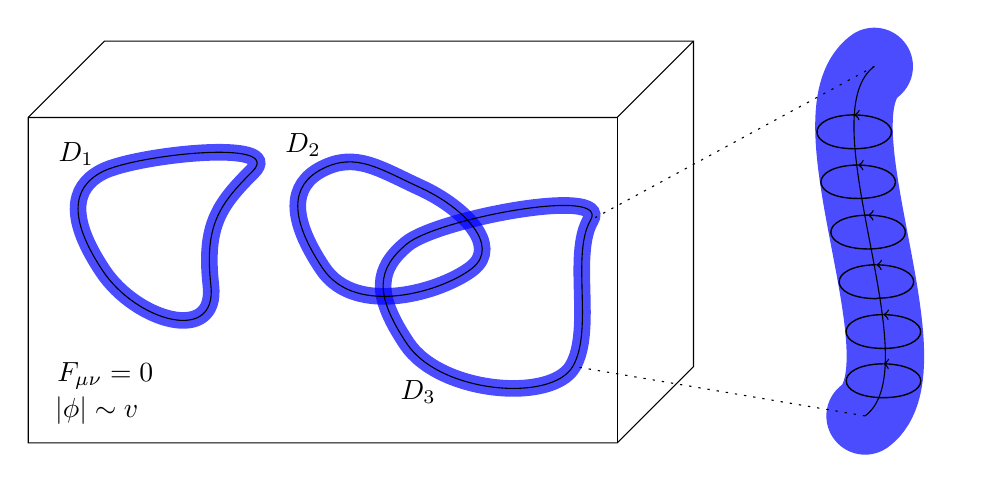
\begin{tikzpicture}[x=0.75pt,y=0.75pt,yscale=-0.8,xscale=0.8]

\draw   [color=blue ,draw opacity=0.7, line width=28, line cap = round] (551,249.25) .. controls (591,219.25) and (516.5,68.75) .. (556.5,38.75) ;
\draw    (551,249.25) .. controls (591,219.25) and (516.5,68.75) .. (556.5,38.75) ;

\draw   (47,69.5) -- (93,23.5) -- (447.67,23.5) -- (447.67,219.5) -- (401.67,265.5) -- (47,265.5) -- cycle ; \draw   (447.67,23.5) -- (401.67,69.5) -- (47,69.5) ; \draw   (401.67,69.5) -- (401.67,265.5) ;

\draw   [->][line width=0.5pt] (557.73,158.2) .. controls (527.89,158.61) and (527.89,178.45) .. (557.89,178.61)(557.89,178.36) .. controls (587.29,178.28) and (587.88,159.23) .. (557.73,158.2) ;
\draw   [->][line width=0.5pt]  (562,217.83) .. controls (532.17,218.25) and (532.17,238.08) .. (562.17,238.25) .. controls (591.57,237.92) and (592.15,218.87) .. (562,217.83);
\draw    [->][line width=0.5pt]  (561.91,188.2) .. controls (532.08,188.61) and (532.08,208.45) .. (562.08,208.61) .. controls (591.48,208.28) and (592.06,189.23) .. (561.91,188.2) ;
\draw    [->][line width=0.5pt]  (552.73,128.29) .. controls (522.89,128.7) and (522.89,148.54) .. (552.89,148.7) .. controls (582.29,148.37) and (582.88,129.32) .. (552.73,128.29) ;
\draw   [->][line width=0.5pt]  (546.73,98.11) .. controls (516.89,98.52) and (516.89,118.36) .. (546.89,118.27) .. controls (576.29,118.19) and (576.88,99.14) .. (546.73,98.11) ;
\draw   [->][line width=0.5pt]  (544.36,67.92) .. controls (514.53,68.34) and (514.53,88.17) .. (544.53,88.34) .. controls (573.93,88.01) and (574.52,68.96) .. (544.36,67.92) ;

\draw   [color=blue ,draw opacity=0.7, line width=6, line cap = round] (224.33,100.33) .. controls (244.33,90.33) and (258.33,100.33) .. (283.67,112) .. controls (309,123.67) and (331.67,146.67) .. (314.33,160.33) .. controls (297,174) and (244.33,190.33) .. (224.33,160.33) .. controls (204.33,130.33) and (204.33,110.33) .. (224.33,100.33) -- cycle ;
\draw   [color=blue ,draw opacity=0.7, line width=6, line cap = round] (275,145.67) .. controls (293,130.67) and (397.67,110.67) .. (385.67,131.33) .. controls (373.67,152) and (387.67,197.33) .. (375,219.33) .. controls (362.33,241.33) and (295,235.67) .. (275,205.67) .. controls (255,175.67) and (257,160.67) .. (275,145.67) -- cycle ;
\draw   [color=blue ,draw opacity=0.7, line width=6, line cap = round](92,102) .. controls (112,92) and (202,82) .. (182,102) .. controls (162,122) and (153,134.5) .. (157,170.5) .. controls (161,206.5) and (112,192) .. (92,162) .. controls (72,132) and (72,112) .. (92,102) -- cycle ;

\draw   (224.33,100.33) .. controls (244.33,90.33) and (258.33,100.33) .. (283.67,112) .. controls (309,123.67) and (331.67,146.67) .. (314.33,160.33) .. controls (297,174) and (244.33,190.33) .. (224.33,160.33) .. controls (204.33,130.33) and (204.33,110.33) .. (224.33,100.33) -- cycle ;
\draw   (275,145.67) .. controls (293,130.67) and (397.67,110.67) .. (385.67,131.33) .. controls (373.67,152) and (387.67,197.33) .. (375,219.33) .. controls (362.33,241.33) and (295,235.67) .. (275,205.67) .. controls (255,175.67) and (257,160.67) .. (275,145.67) -- cycle ;
\draw   (92,102) .. controls (112,92) and (202,82) .. (182,102) .. controls (162,122) and (153,134.5) .. (157,170.5) .. controls (161,206.5) and (112,192) .. (92,162) .. controls (72,132) and (72,112) .. (92,102) -- cycle ;

\draw  [dash pattern={on 0.84pt off 2.51pt}]  (556.5,38.75) -- (385.67,131.33) ;
\draw  [dash pattern={on 0.84pt off 2.51pt}]  (551,249.25) -- (375,219.33) ;

\draw (63.67,82.8) node [anchor=north west][inner sep=0.75pt]    {$D_{1}$};
\draw (200.33,77.73) node [anchor=north west][inner sep=0.75pt]    {$D_{2}$};
\draw (269.67,226.4) node [anchor=north west][inner sep=0.75pt]    {$D_{3}$};
\draw (63,215.4) node [anchor=north west][inner sep=0.75pt]    {$F_{\mu \nu } =0$};
\draw (61.67,236.4) node [anchor=north west][inner sep=0.75pt]    {$| \phi | \sim v$};
\end{tikzpicture}
\caption{Defects (blue closed lines) and their loci (black closed lines). On the right side of the picture, is represented in more detail the vortex associated to the defect $D_3$.}
\label{fig:defects-vortex}
\end{figure}

In order to understand how to ``open'' these line defects, let's first consider the restriction of the field strength $F$ of the vortex to a 2 dimensional disk crossing transversally the locus of the defect, such that the boundary of the disk identify the region where the configuration approximately approaches the vacuum one, as represented in fig.~\ref{fig:disk-defect}. 

\begin{figure}[h]
\centering

\tikzset{
pattern size/.store in=\mcSize, 
pattern size = 6pt,
pattern thickness/.store in=\mcThickness, 
pattern thickness = 0.3pt,
pattern radius/.store in=\mcRadius, 
pattern radius = 0pt}
\makeatletter
\pgfutil@ifundefined{pgf@pattern@name@EllipsePattern}{
\pgfdeclarepatternformonly[\mcThickness,\mcSize]{EllipsePattern}
{\pgfqpoint{0pt}{0pt}}
{\pgfpoint{\mcSize+\mcThickness}{\mcSize+\mcThickness}}
{\pgfpoint{\mcSize}{\mcSize}}
{
\pgfsetcolor{\tikz@pattern@color}
\pgfsetlinewidth{\mcThickness}
\pgfpathmoveto{\pgfqpoint{0pt}{0pt}}
\pgfpathlineto{\pgfpoint{\mcSize+\mcThickness}{\mcSize+\mcThickness}}
\pgfusepath{stroke}
}}
\makeatother
\tikzset{every picture/.style={line width=0.75pt}} %set default line width to 0.75pt        

\begin{tikzpicture}[x=0.75pt,y=0.75pt,yscale=-0.6,xscale=0.6]
%uncomment if require: \path (0,300); %set diagram left start at 0, and has height of 300

%Curve Lines [id:da33705367027161603] 
\draw   [color=blue ,draw opacity=0.7, line width=21, line cap = round] (571,269.25) .. controls (611,239.25) and (536.5,88.75) .. (576.5,58.75) ;
\draw   (571,269.25) .. controls (611,239.25) and (536.5,88.75) .. (576.5,58.75) ;

%Curve Lines [id:da21282626058718623] 
\draw   [->][line width=0.5pt] (577.73,178.2) .. controls (547.89,178.61) and (547.89,198.45) .. (577.89,198.61) .. controls (607.29,198.28) and (607.88,179.23) .. (577.73,178.2) ;
%Curve Lines [id:da8259045720854306] 
\draw   [->][line width=0.5pt] (582,237.83) .. controls (552.17,238.25) and (552.17,258.08) .. (582.17,258.25) .. controls (611.57,257.92) and (612.15,238.87) .. (582,237.83) ;
%Curve Lines [id:da00807708837653065] 
\draw   [->][line width=0.5pt] (581.91,208.2) .. controls (552.08,208.61) and (552.08,228.45) .. (582.08,228.36) .. controls (611.48,228.28) and (612.06,209.23) .. (581.91,208.2) ;
%Curve Lines [id:da9551996169478982] 
\draw  [->][line width=0.5pt]  (572.73,148.29) .. controls (542.89,148.7) and (542.89,168.54) .. (572.89,168.45) .. controls (602.29,168.37) and (602.88,149.32) .. (572.73,148.29) ;
%Curve Lines [id:da6438432478749674] 
\draw   [->][line width=0.5pt] (566.73,118.11) .. controls (536.89,118.52) and (536.89,138.36) .. (566.89,138.27) .. controls (596.29,138.19) and (596.88,119.14) .. (566.73,118.11) ;
%Curve Lines [id:da09026447567603135] 
\draw  [->][line width=0.5pt]  (564.36,87.92) .. controls (534.53,88.34) and (534.53,108.17) .. (564.53,108.34)(564.53,108.09) .. controls (593.93,108.01) and (594.52,88.96) .. (564.36,87.92) ;
%Shape: Ellipse [id:dp059940750148450794] 
\draw  [color=red][pattern=EllipsePattern, pattern color=red] [dash pattern={on 1pt off 0.5pt}, line width=0.5] (502.9,158.25) .. controls (502.9,136.16) and (534.24,118.25) .. (572.9,118.25) .. controls (611.56,118.25) and (642.9,136.16) .. (642.9,158.25) .. controls (642.9,180.34) and (611.56,198.25) .. (572.9,198.25) .. controls (534.24,198.25) and (502.9,180.34) .. (502.9,158.25) -- cycle ;

\draw (572.5,158.25) circle (1pt)[color=red, fill=red] ;

\end{tikzpicture}
\caption{Disk crossing the locus of the defect, whose boundary identify the region where the configuration approaches the vacuum.}
\label{fig:disk-defect}
\end{figure}

We then identify the points of the boundary to one-point, obtaining a closed 2-dimensional surface $S^2$, as represented in fig.~\ref{fig:compactification-Riemann-sphere}. 

\begin{figure}[h]
\centering
\def\svgwidth{\columnwidth}
\scalebox{0.5}{\adjustbox{trim={.0\width} {.15\height} {0.\width} {.32\height},clip}{\input{../img/riemann-sphere.pdf_tex}}}
\caption{Compactification of the plane by identification of the boundaries. Source: \url{https://demonstrations.wolfram.com/TheRiemannSphereAsAStereographicProjection/}}
\label{fig:compactification-Riemann-sphere}
\end{figure}

According to our previous discussion,
\begin{eq}\label{eq:vorticity-compact-disk-in}
	\frac1{2\pi}\int_{S^2}F_{\mu\nu}\de S^{\mu\nu} = n = \text{vorticity carried by the defect $D$}
\end{eq}
Let's see how $A_\mu$ behaves on such sphere. Using definition eq.~\eqref{eq:map-e-phi-vortex}, we get
\begin{eq}
	D_\mu\phi&=e^{i\theta}\partial_\mu|\phi|+|\phi|e^{i\theta}(e^{-i\theta}\partial_\mu e^{i\theta}-iA_\mu)\\
	(D_\mu\phi)^*&=e^{-i\theta}\partial_\mu|\phi|+|\phi|e^{-i\theta}(e^{i\theta}\partial_\mu e^{-i\theta}+iA_\mu)
\end{eq}
where we set $n_ee=1$ in order to get rid of these coefficients. Hence we obtained\todo{Come mai il secondo termine può esser singolare?}
\begin{eq}
	A_\mu=\underbrace{\vphantom{\int_T}\frac i2\frac{e^{-i\theta}D_\mu\phi-e^{i\theta}(D_\mu\phi)^*}{|\phi|}}_{\text{regular term}}+\underbrace{\vphantom{\int_T}\frac i2(e^{i\theta}\partial_\mu e^{-i\theta}-e^{-i\theta}\partial_\mu e^{i\theta})}_{\text{singular term}}
\end{eq}
Recall that $\theta(x)$ is an angle around the center of the vortex, where $|\phi|=0$. Without loss of generality we can assume that the center of the vortex coincide with the origin of the space. In the sense of distributions, the field strength of the singular term above is
\begin{eq}
	\lctens^{\mu\nu}\partial_\mu\left(\frac i2(e^{i\theta}\partial_\mu e^{-i\theta}-e^{-i\theta}\partial_\mu e^{i\theta})\right)
	=\frac1i\lctens^{\mu\nu}\partial_\mu\partial_\nu\log e^{i\theta}=2\pi\delta(\vec x)
\end{eq}
since the dependence of $\theta$ on the space coordinates goes with $\arctan\frac yx$. Hence such field strength is non zero (actually, singular) only in the center of the vortex. Therefore the complete field strength of $A_\mu$ is\todo{Che cos'è $a_\nu$? Forse intendeva $A_\nu$? Inoltre ho visto che nelle note ha modificato la formula data a lezione, volevo chiederle quale fosse la versione corretta (stessa cosa anche per la formula precedente).}
\begin{eq}
	F_{\mu\nu}(\vec x)=\partial_{[\mu}a_{\nu]}(\vec x)+2\pi\delta(|\phi|)\lctens_{\mu\nu}
\end{eq}
so that the support of $F_{\mu\nu}$ is given by the loci of defects, i.e. where $|\phi|=0$.

We see then that one can identify the locus of the defect in $F_{\mu\nu}$ in terms of a ``singular current'' (i.e. ``$\delta$-like'') in the support where $|\phi|$ vanishes, which is necessarily closed because the boundary condition at infinity is $|\phi|=v$. 

\subsubsection{Open defects}

If we want to open a defect and $\vec x$ is a boundary of the locus of such defect, we need to construct a 2-tensor $F_{\mu\nu}^{\vec x}$ such that for a surface $S_{\vec x}^2$ centered at $\vec x$ and of arbitrarily small radius we have 
\begin{eq}
	\int_{S_{\vec x}^2}F_{\mu\nu}^{\vec x}\de x^\mu\de x^\nu=2\pi n
\end{eq}
and then if $B_{\vec x}^3$ is the ball centered in $\vec x$ whose boundary is $S^2_{\vec x}$, by Gauss theorem we have
\begin{eq}
	\int_{S^2_{\vec x}}F_{\mu\nu}^{\vec x}\de x^\mu\de x^\nu=\int_{B^3_{\vec x}}\lctens^{\mu\nu\rho}\partial_\mu F_{\nu\rho}^{\vec x}\de^3x=2\pi n
\end{eq}
which should hold for any arbitrarily small radius, so that
\begin{eq}
	\lctens^{\mu\nu\rho}\partial_\mu F_{\nu\rho}^{\vec x}(\vec y)=2\pi n\,\delta(\vec x-\vec y)
\end{eq}
or equivalently, using $\lctens^{\mu\nu\rho}F_{\nu\rho}^{\vec x}=B^\mu_{\vec x}$ where $B^\mu_{\vec x}$ is the magnetic field centered at $\vec x$, 
\begin{eq}\label{eq:vorticity-compact-disk-bc}
	\big(\vec\nabla\cdot\vec B_{\vec x}\big)(\vec y)=2\pi n\,\delta(\vec x-\vec y)
\end{eq}
This is precisely the magnetic field of a \emph{monopole} in $\R^3$, i.e. the analogue of a point-like electric charge of charge $q$ which obeys
\begin{eq}
	\big(\vec\nabla\cdot\vec E_{\vec x}\big)(\vec y)=q\,\delta(\vec x-\vec y)
\end{eq}
with the magnetic field replacing the electric field. 

Therefore we can build open defects constructing line defects with monopoles at the boundaries. Respect to fig.~\ref{fig:disk-defect}, this is equivalent to the introduction of two compactified disks (hence they actually are 2-spheres) at the boundaries of the line, describing classical monopoles, as represented in fig.~\ref{fig:open-defect-vortex}. Comparing eq.~\eqref{eq:vorticity-compact-disk-in} and eq.~\eqref{eq:vorticity-compact-disk-bc} we see that such monopoles ``provide the right vorticity'' to the defect. 

\begin{figure}[h]
\centering
\tikzset{every picture/.style={line width=0.75pt}}     
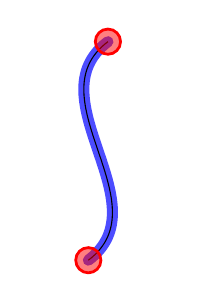
\begin{tikzpicture}[x=0.75pt,y=0.75pt,yscale=-0.9,xscale=0.9]

%Curve Lines [id:da8908477525317537] 
\draw   [color=blue ,draw opacity=0.7, line width=4, line cap = round] (31,141.5) .. controls (71,111.5) and (1.5,54.5) .. (41.5,24.5) ;
\draw    (31,141.5) .. controls (71,111.5) and (1.5,54.5) .. (41.5,24.5) ;
%Shape: Circle [id:dp297621710933869] 
\draw  [color=red, line width=1, fill=red, fill opacity=0.5] (24.25,141.5) .. controls (24.25,137.77) and (27.27,134.75) .. (31,134.75) .. controls (34.73,134.75) and (37.75,137.77) .. (37.75,141.5) .. controls (37.75,145.23) and (34.73,148.25) .. (31,148.25) .. controls (27.27,148.25) and (24.25,145.23) .. (24.25,141.5) -- cycle ;
%Shape: Circle [id:dp807790352207095] 
\draw  [color=red, line width=1, fill=red, fill opacity=0.5] (34.75,24.5) .. controls (34.75,20.77) and (37.77,17.75) .. (41.5,17.75) .. controls (45.23,17.75) and (48.25,20.77) .. (48.25,24.5) .. controls (48.25,28.23) and (45.23,31.25) .. (41.5,31.25) .. controls (37.77,31.25) and (34.75,28.23) .. (34.75,24.5) -- cycle ;

\end{tikzpicture}
\caption{Representation of an open defect, whose boundaries are described by monopoles (red circles).}
\label{fig:open-defect-vortex}
\end{figure}

\subsubsection{Correlators}

Similarly to what we have done for the kink, where we modified the action introducing a new parallel transporter to construct the open defects, now we should insert classical monopoles in the action at the positions in which we want to find the creation or the annihilation of the quantum vortices of our theory. Correlators of the quantum vortex field will have insertion points at the monopoles positions. 

%%%%%%%%%%%%%%%%%%%%%%%
%%%%%%%% LECTURE 19 %%%%%%%%
%%%%%%%%%%%%%%%%%%%%%%%

%%%%%%%%%%%%%%%%%%%%%%%
%%%%%%%% LECTURE 20 %%%%%%%%
%%%%%%%%%%%%%%%%%%%%%%%

\end{document}